\usepackage{lipsum}

\begin{document}

% =======================================================================================
%\cleardoublepage % Forces the first chapter to start on an odd page so it's on the right

% =======================================================================================
%                                   PREAMBLE
% =======================================================================================
\coverpage{\TITLE}{\SUBTITLE}{\AUTHOR}{\DATE}{\SUBJECT}
%----------------------------------------------------------------------------------------

\newpage

\paragraph{Abstract}

One of the growing areas of computational intelligence is automatic programming, where a learning algorithm produces executable software. This paradigm promises efficient and highly capable artificial intelligence agents that express their knowledge and reasoning process in a programming language that can be understood, audited and edited by humans, as well as other automated tools - essential requirements for decision support systems in safety-critical application areas such as healthcare.

Of particular interest for healthcare is Programmatically Interpretable Reinforcement Learning, in which a program induction algorithm is used to search for a protocol that performs well in a predictive patient simulator.
The simulator can be derived from clinical data, implemented based on expert knowledge or combine both methods.
Deployment of this approach in real world settings is hindered by the lack of specialized patient simulators and insufficient capabilities of modern program synthesis algorithms.
This work makes contributions to both fields.

The contributions to synthesis algorithms are a novel programming language for general purpose neural program synthesis, a neurogenetic programming framework for program synthesis in BF++ or similar simple languages, a tree variational autoencoder model for code and, finally, Synthesize Execute Debug and Rank: a state-of-the-art iterative algorithm for fully autonomous programming with large language models.

In the field of patient simulators, an anthropodidactic Reinforcement Learning environment for emergency care (Auto-ALS) is introduced, a framework for image-based sonography simulators and a benchmark dataset for intensive care simulation. 

The proposed program synthesis algorithms are evaluated on standard benchmarks as well as Auto-ALS to identify healthcare-specific insights.
The advances introduced in this work lay the foundations for the nascent field of Programmatically Interpretable Reinforcement Learning for Healthcare.

\tableofcontents

\addcontentsline{toc}{section}{List of Figures}
\listoffigures

\addcontentsline{toc}{section}{List of Tables}
\listoftables

\addcontentsline{toc}{section}{Nomenclature}
\nomenclature{PBE}{Programming by example \cite{gulwani2016:programming, halbertProgrammingExample1984}}
\nomenclature{PIRL}{Programmatically Interpretable Reinforcement Learning \cite{pirl}}
\nomenclature{PatientSPIRL}{Patient Simulator Programmatically Interpretable Reinforcement Learning, introduced in chapter \ref{ch:proposal}}

\nomenclature{RL}{Reinforcement Learning \cite{suttonReinforcementLearningSecond2018}}
\nomenclature{PQT}{Priority Queue Training \cite{abolafiaNeuralProgramSynthesis2018}}
\nomenclature{POMDP}{Partially Observable Markov Decision Process \cite{kramerjdavidrPartiallyObservableMarkov1964}}
\nomenclature{MPC}{Model Predictive Control \cite{garciaModelPredictiveControl1989, holkarOverviewModelPredictive2010, kouvaritakisModelPredictiveControl2016, schwenzerReviewModelPredictive2021}}
\nomenclature{MDPD}{Message Passing Decision Process, introduced in section \ref{sec:mpdp}}

\nomenclature{GPT}{Generative Pre-trained Transformer \cite{radfordImprovingLanguageUnderstandinga}}
\nomenclature{LLM}{Large Language Model}
\nomenclature{AI}{Artificial Intelligence}

\nomenclature{CASE}{Computer-Aided Software Engineering \cite{ComputeraidedSoftwareEngineering2025}}
\nomenclature{AST}{Abstract Syntax Tree, see \ref{sec:grammar-guided}}

\nomenclature{SEIDR}{Synthesize Execute Debug Rank, introduced in chapter \ref{ch:seidr}}

\nomenclature{MHE}{Moving Horizon Estimator}

\nomenclature{CAPFT}{Capacity modifier function with temperature}
\nomenclature{CO2}{Carbon dioxide}
\nomenclature{EIR}{Energy input ratio}
\nomenclature{EIRFT}{Energy input ratio function with temperature}
\nomenclature{EIRFPLR}{Energy input ratio function with partial load ratio}
\nomenclature{HVAC}{Heating Ventilation Air Conditioning}
\nomenclature{IDEAS}{Integrated District Energy Assessment Simulations}
\nomenclature{IPOPT}{Interior Point Optimizer}
\nomenclature{KPI}{Key Performance Indicator}
\nomenclature{PI}{Proportional Integral}
\nomenclature{PLR}{Partial load ratio}
\nomenclature{RC}{Resistance capacitance}

\nomenclature{ALS}{Advanced Life Support \cite{AMLSAdvancedMedical2021}}

\newcommand{\obs}{\mathbf{o}}
\nomenclature{$\obs$}{a single observation of an agent}

\newcommand{\policy}{\pi}
\nomenclature{$\policy(\action)$}{a \emph{policy distribution} that stochastically defines the agent's actions}
\nomenclature{$\policy(\text{text})$}{language model (probability distribution over texts)}

\newcommand{\discretebins}{\Upsilon^\text{bins}}
\nomenclature{$\discretebins$}{number of discretization bins}

\newcommand{\historylen}{\Upsilon^\text{history}}
\nomenclature{$\historylen$}{history length, the number of past steps considered by the algorithm}

\newcommand{\mlinput}{x}
\newcommand{\mlinputvec}{\mathbf{x}}
\nomenclature{$\mlinput$, $\mlinputvec$}{input examples in a machine learning system}

\newcommand{\step}{i}
\newcommand{\stepp}{j}
\newcommand{\steppp}{k}
\nomenclature{$\step$,$\stepp$,$\steppp$}{iteration, step, moment in discrete time}

\newcommand{\mloutput}{y}
\newcommand{\mloutputvec}{\mathbf{y}}
\nomenclature{$\mloutput$, $\mloutputvec$}{expected output examples in a machine learning system}

\newcommand{\obss}{\mathcal{O}}
\nomenclature{$\obss$}{set of all possible observations $\obs$}

\newcommand{\state}{\textbf{s}}
\nomenclature{$\state$}{a state of an environment}

\newcommand{\states}{\mathcal{S}}
\nomenclature{$\states$}{set of all possible states $\state$ of an environment}

\newcommand{\termstates}{\mathcal{S}_t}
\nomenclature{$\termstates$}{set of all terminal states $\state$ of an environment}

\newcommand{\nontermstates}{\mathcal{S}_{nt}}
\nomenclature{$\nontermstates$}{set of all non-terminal states $\state$ of an environment}

\newcommand{\action}{a}
\nomenclature{$\action$}{an action of an agent}

\newcommand{\actions}{\mathcal{A}}
\nomenclature{$\actions$}{set of all possible actions $\action$}

\newcommand{\actionqueue}{\alpha}
\nomenclature{$\actionqueue$}{action queue of an agent}

\newcommand{\reward}{r}
\nomenclature{$\reward$}{a reward}

\newcommand{\returnn}{R_n}
\nomenclature{$\returnn$}{n-step return}

\newcommand{\returntot}{R_\text{tot}}
\nomenclature{$\returntot$}{total episode return}

\newcommand{\realnums}{\mathbb{R}}
\nomenclature{$\realnums$}{real numbers}

\newcommand{\memory}{m}
\nomenclature{$\memory$}{memory of an agent}

\newcommand{\alphabet}{\aleph}
\nomenclature{$\alphabet$}{the alphabet of a programming language (set of all possible tokens $\token$)}

\newcommand{\token}{c}
\nomenclature{$\token$}{a \emph{token}, a minimal unit of code, such as a character}

\newcommand{\code}{\mathcal{C}}
\nomenclature{$\code$}{\emph{program code}, a sequence of tokens $\token_1,\token_2,\dots$ that constitutes a program}

\newcommand{\codebase}{\kappa}
\nomenclature{$\codebase$}{\emph{codebase}, a population of programs}

\newcommand{\expectation}{\mathbb{E}}
\nomenclature{$\expectation$}{expected value}

\newcommand{\loss}{\lambda}
\nomenclature{$\loss(x)$}{a differentiable loss function to be minimized by an optimization algorithm}

\newcommand{\obj}{\omega}
\nomenclature{$\obj(x)$}{an objective function to be maximized by an optimization algorithm}

\newcommand{\learnables}{\Phi}
\nomenclature{$\learnables$}{learnable parameters of a model}

\newcommand{\weights}{\mathbf{W}}
\nomenclature{$\weights$}{weight matrix in a model, element of $\learnables$}

\newcommand{\biases}{\mathbf{b}}
\nomenclature{$\biases$}{bias vector in a model, element of $\learnables$}

\newcommand{\hidden}{\mathbf{h}}
\nomenclature{$\hidden$}{a hidden state within a model}

\newcommand{\latent}{\mathbf{z}}
\nomenclature{$\latent$}{a latent representation of input $\mlinput$}

\newcommand{\mean}{\mu}
\nomenclature{$\mean$}{mean}

\newcommand{\variance}{\sigma}
\nomenclature{$\variance$}{variance}

\newcommand{\normaldistr}{\nu}
\nomenclature{$\normaldistr(\mu,\sigma)$}{the normal distribution}

\newcommand{\pointer}{P}
\nomenclature{$\pointer$}{pointer}

\newcommand{\prob}{p}
\nomenclature{$\prob$}{probability}

\newcommand{\team}{\Xi}
\nomenclature{$\team$}{a cooperative \emph{team} of agents}

\newcommand{\temp}{T}
\nomenclature{$\temp$}{sampling temperature}
\nomenclature{$\temp$}{physical temperature}

\newcommand{\timepoint}{t}
\nomenclature{$\timepoint$}{a moment in continuous time}

\newcommand{\threshold}{\theta}
\nomenclature{$\threshold$}{threshold value for discretization}

\newcommand{\hyperparam}{\Upsilon}
\nomenclature{$\Upsilon$}{hyperparameter of an algorithm}

\newcommand{\beamwidth}[0]{\hyperparam^\text{beam}}
\nomenclature{$\beamwidth$}{beam width in beam search}

\newcommand{\treearity}[0]{\hyperparam^\text{tree}}
\nomenclature{$\treearity$}{tree arity, as in $\treearity$-ary tree}

\newcommand{\integers}{\mathbb{Z}}
\nomenclature{$\integers$}{integers}

\printnomenclature

\emph{A note on notation:} bold lowercase characters $\mathbf{x}$ represent vectors, bold uppercase characters $X$ represent matrices, calligraphic letters $\mathcal{X}$ represent sets and tuples. This holds for functions as well, i.e. $f(\mathbf{x})$ maps vectors to scalars
\printnomenclature

\newpage
\chapter{Deep Program Induction} \label{ch:autocode-motiv}
\chapter{Background: Deep Program Induction} 
\label{ch:promise}

\section{The Quest of Automatic Programming}

\label{sec:quest}

\emph{Automatic programming} or \emph{program synthesis} refers to any technological setup wherein the task of writing computer programs is automated. 
First introduced in science fiction \cite{jenkinsLogicNamedJoe1946}, it is now an active area of technical research.
Program synthesis systems are defined by what type of task \emph{specification} they admit, whether and how the generated programs are verified, whether and how pre-existing programs are incorporated \cite{gulwaniDimensionsProgramSynthesis2010}:

\begin{figure}[H]
    \centering
    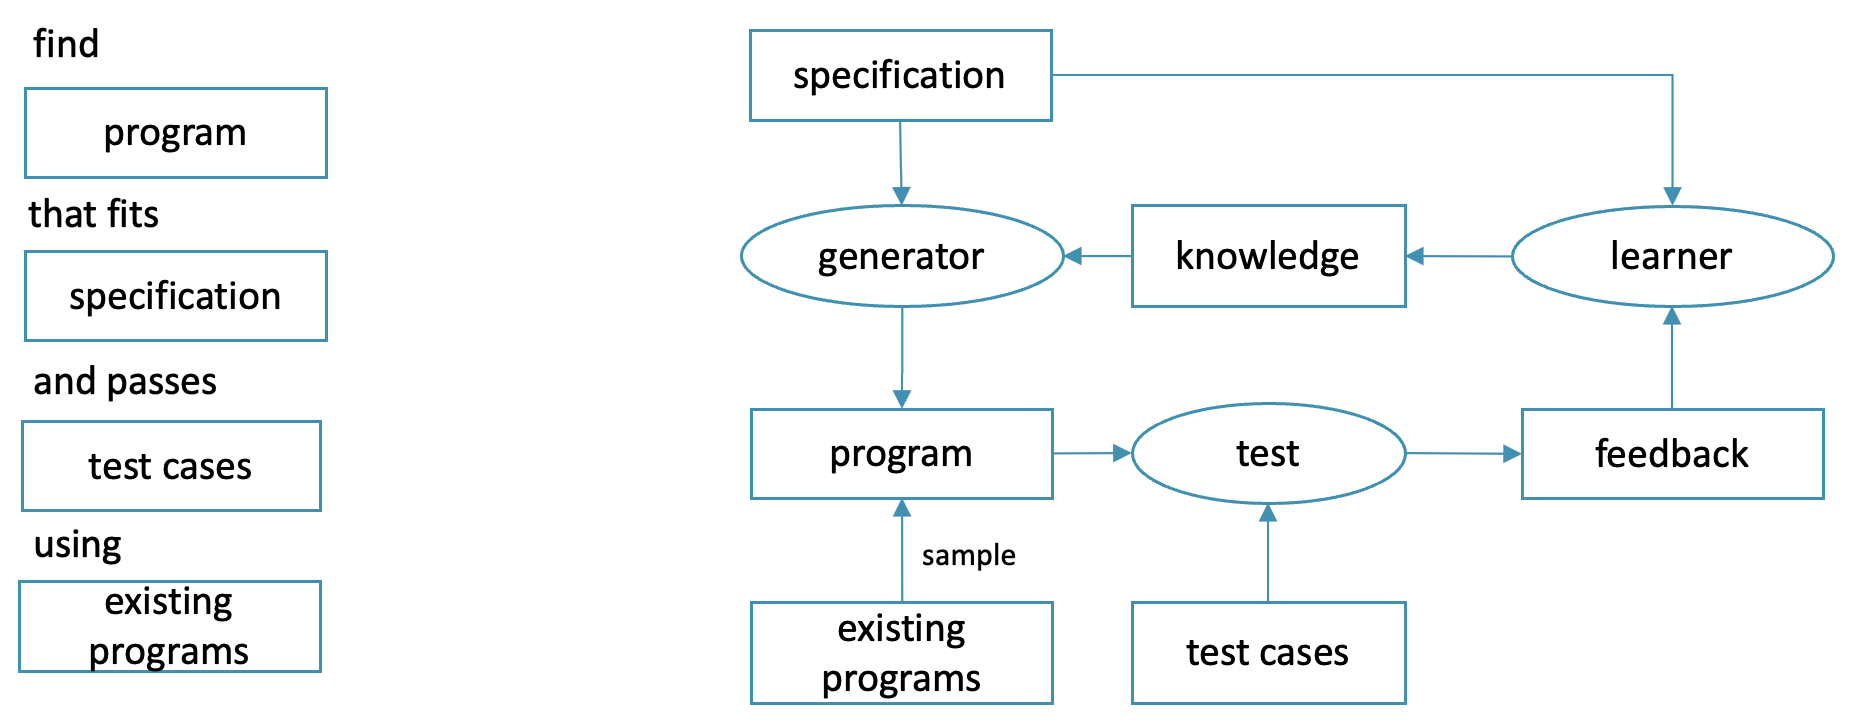
\includegraphics[width=\linewidth]{ap.png}
    \caption{Automatic programming system, schematic definition}
    \label{fig:ap}
\end{figure}

This definition in figure \ref{fig:ap} is purposefully broad and includes, for example, the compiler (figure \ref{fig:compiler}) \cite{penjamDeductiveInductiveMethods2003,patrickmckenzie[@patio11]GlibLineHave2023}: a program synthesis system that turns a specification in the form of a program in a programming language designed for ease of use by humans into a program in a programming language designed for ease of deployment on a computer.

\begin{figure}[H]
    \centering
    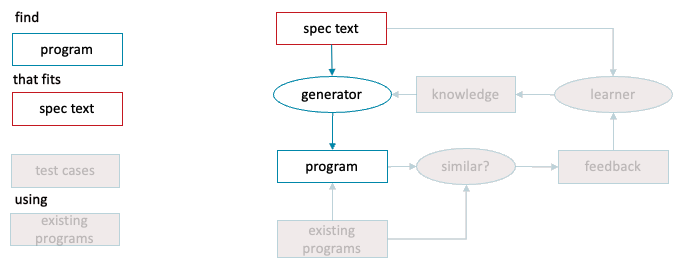
\includegraphics[width=\linewidth]{compiler.png}
    \caption{Compiler, schematic definition}
    \label{fig:compiler}
\end{figure}

The ambition of the field, however, extends far beyond compilers \cite{campbellAutomatedCodingQuest2020}.
The goal is to impose as few constraints as possible onto the \emph{specification} and ultimately automate the generation of programs for any free-form specification, such as a short textual \cite{zanLargeLanguageModels2023} prompt or a diagram \cite{koziolekLLMbasedControlCode2023}, even a hand-drawn sketch \cite{chatgptmodderChatgptCanNow2023}.

% TODO: examples for the above

\newpage
\section{Taxonomy of tasks}
\label{sec:taxonomy}

\paragraph{Code translation}

The humble compiler from section \ref{sec:quest} is an instance of a \emph{code translation} system: a \emph{program synthesis} system where the specification is given as text, either in a natural language (\emph{NL2Code translation} \cite{wangNaturalLanguageCode2023, zanLargeLanguageModels2023}) or in a programming language (\emph{code2code translation} \cite{radfordImprovingLanguageUnderstanding})
Code to natural language translation is studied as well \cite[section 5.1]{leDeepLearningSource2020}, but it is less common and out-of-scope for this work.
Intelligent conversational assistants (\href{https://chat.openai.com/}{ChatGPT}, \href{https://gemini.google.com}{Gemini}, \href{https://claude.ai/}{Claude}, \href{https://pi.ai/}{Pi}) with program synthesis functionality operate in the translation paradigm as they translate a text specification into code.

\begin{figure}[H]
    \centering
    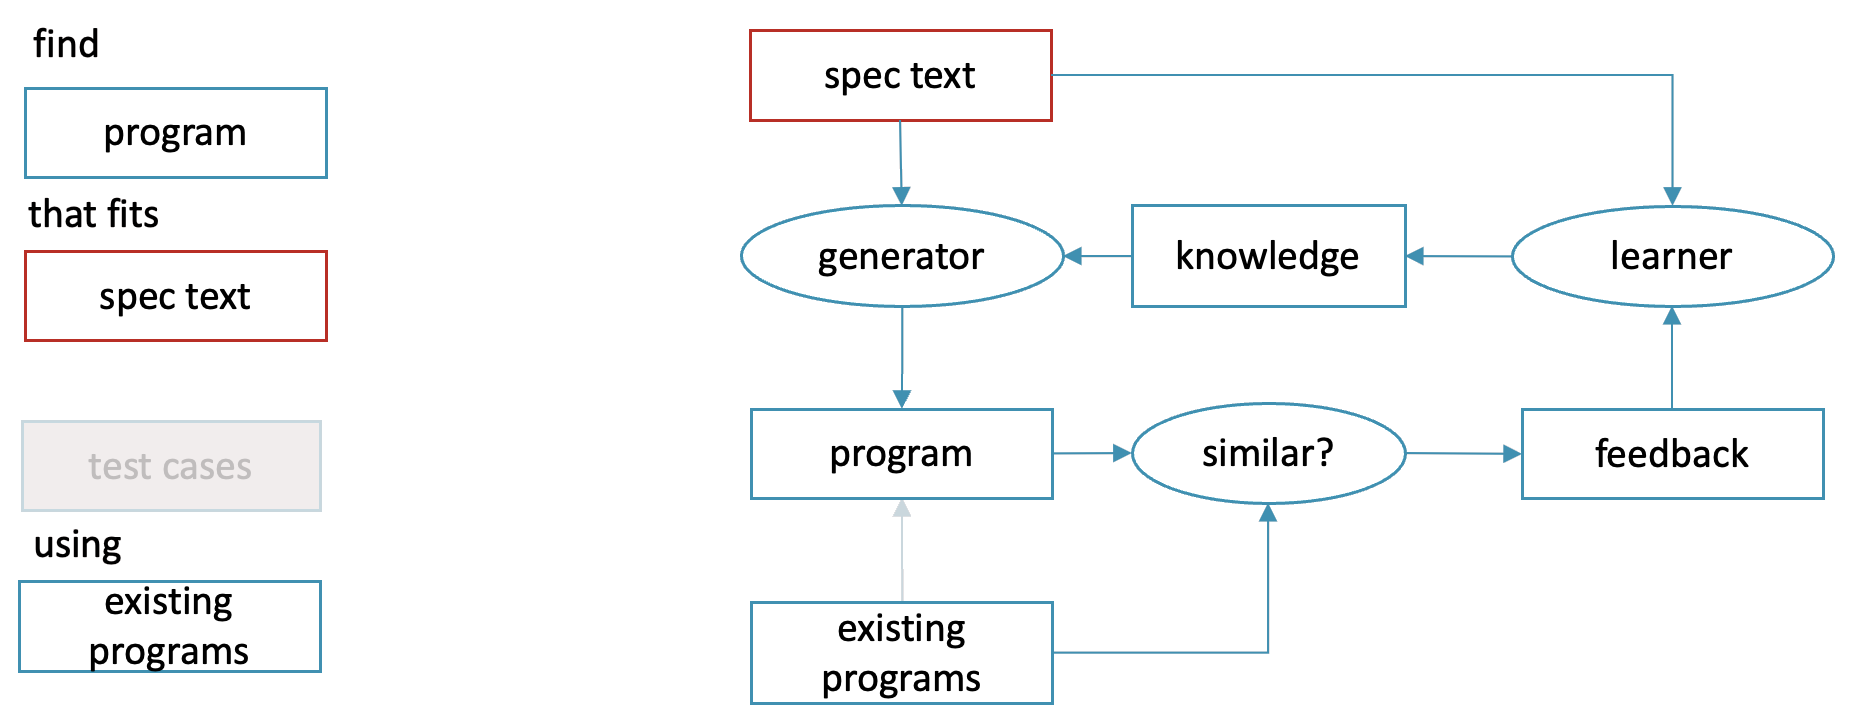
\includegraphics[width=\linewidth]{nl2ml.png}
    \caption{Code translation, schematic definition}
    \label{fig:nl2ml}
\end{figure}

\paragraph{Programming by example}

Another approach to specification is specifying the expected output of the program. Or, since in most interesting programs the output depends on the input, \emph{input-output pairs}. This task is known as \emph{programming by example} \cite{halbertProgrammingExample1984, psb2}.

\begin{figure}[H]
    \centering
    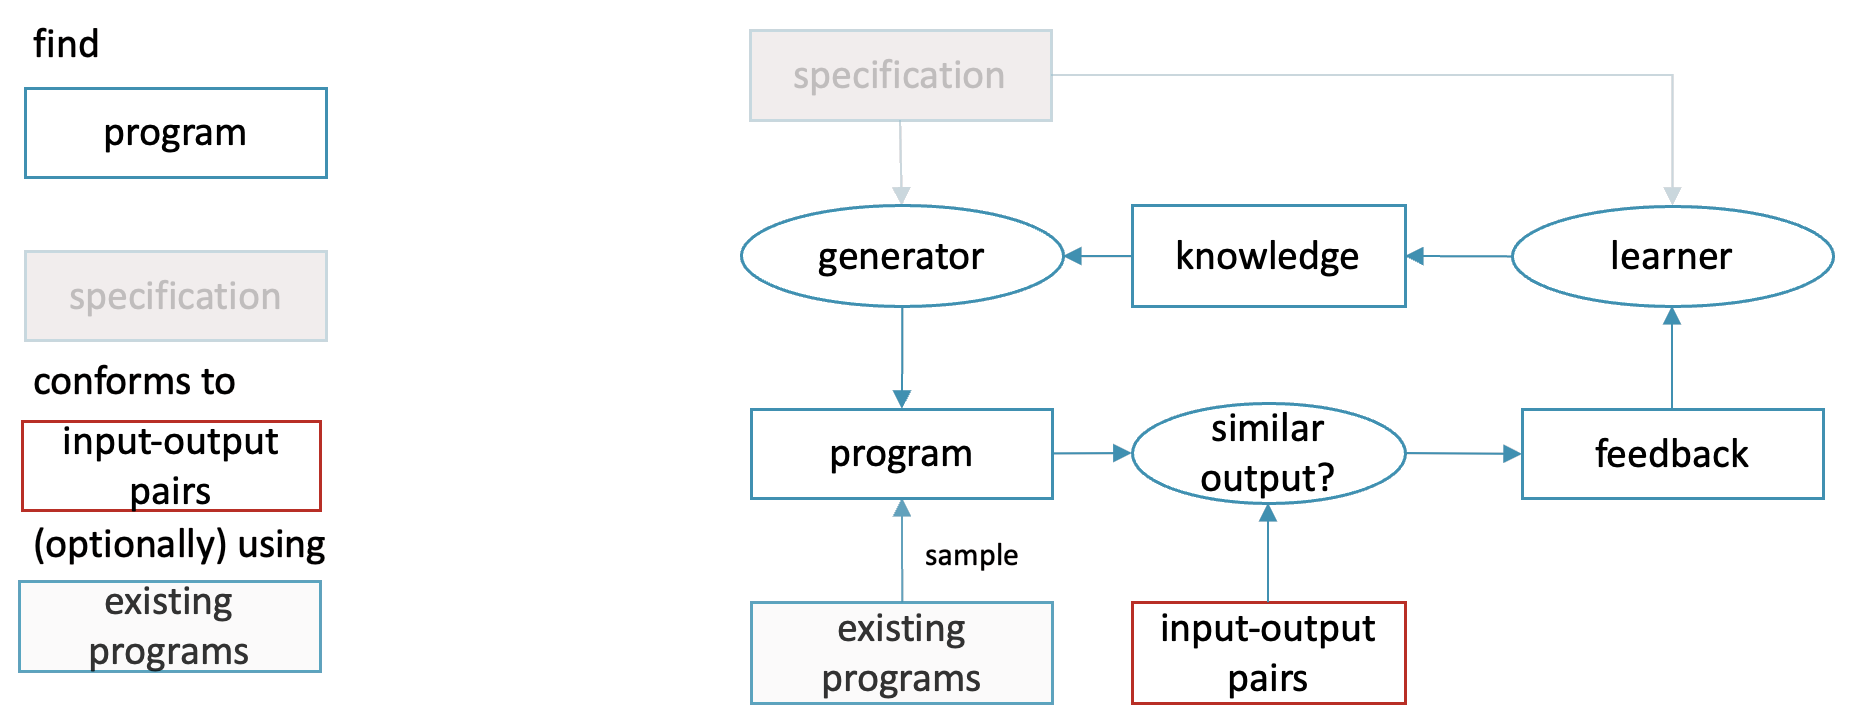
\includegraphics[width=\linewidth]{pbe.png}
    \caption{Programming by example, schematic definition}
    \label{fig:pbe}
\end{figure}

The goal of a programming by example system is to find a program $f$ such that $\outputvec=f(\inputvec)$ for a given vector of input-output pairs $(\inputvec,\outputvec)$. 
Note that this is exactly the definition of \emph{supervised learning}~\cite{cunninghamSupervisedLearning2008}.
Indeed, \emph{programming by example} is an unusual type of \emph{supervised learning}, one where the trained model is expressed as source code.

The prime application of \emph{programming by example} is \emph{data wrangling} tools such as Microsoft Excel \cite{gulwaniProgrammingExamplesandIts2016} where it is used as a data extrapolation tool: if a formula $f$ can be synthesized that satisfies $\outputvec=f(\inputvec)$, one can generate $\outputvec '=f(\inputvec ')$ for future values $\inputvec '$.
\emph{Programming by example} is also used in scientific domains to generate formulas that fit experimental observations, where it is known as \emph{symbolic regression} \cite{makkeInterpretableScientificDiscovery2022}.

\paragraph{PIRL}

Not every task, however, can be easily described with input-output examples. 
Take chess: it's relatively simple to evaluate the performance of a chess-playing program, but what are the \emph{correct} moves? 
That is simply not known in advance.
Given enough trial and error it's still possible to generate a correct program with such black box specification, a task known as \emph{Programmatically Interpretable Reinforcement Learning} \cite{pirl}.

\begin{figure}[H]
    \centering
    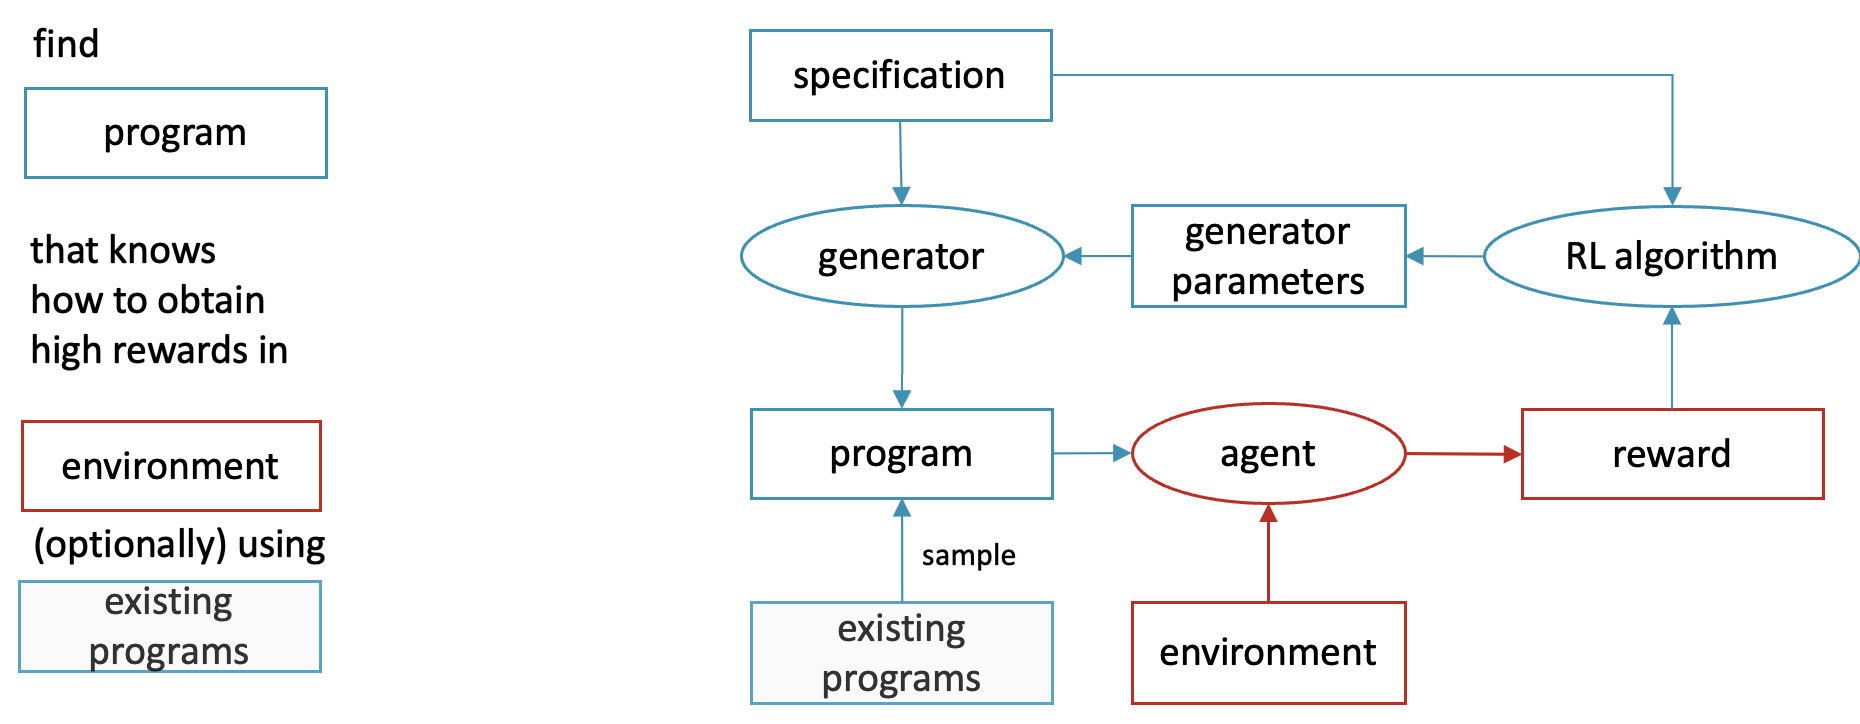
\includegraphics[width=\linewidth]{pirl.png}
    \caption{Programmatically Interpretable Reinforcement Learning, schematic definition}
    \label{fig:pirl}
\end{figure}

In this setting, a program gets generated and deployed in an environment that responds with positive and negative rewards. 
The most common formalism for such an environment as Partially Observable Markov Decision Process \cite{kramerjdavidrPartiallyObservableMarkov1964, spaanPartiallyObservableMarkov2012}: when at step $i$ the agent takes action $a_i \in \rlactions$ it has an impact on  the state of the environment $s_i \in \rlstates$ via distribution $\rlstatedistr$ of conditional probabilities of possible subsequent states. 
State is a latent variable that the agent cannot observe.
Instead, the agent can see an observation $o_i \in \rlobss$ which is a random variable that depends on the latent state via distribution $\rlobsdistr$.
$\rlactions$, $\rlstates$ and $\rlobss$ are sets of all possible actions, states and observations respectively.
Finally, at every step the agent observes a reward $\rlrewardf$

Given this limited toolset, without full (or any) prior knowledge of how the agent's actions influence the the environment (distributions $\rlstatedistr$ and $\rlobsdistr$), the agent has to come up with a strategy that will maximize $n$-step return $R_n=\sum_{t=i}^{n} r_t$ where $n$ is the agent's planning horizon. It is, in the general sense, a hyperparameter, however if an environment has a limit on how many steps an episode can last, it is reasonable to set $n$ equal to the step limit. 

\newpage
\section{Why not just use Machine Learning?}

As programmatically interpretable cousins of \emph{supervised learning} and \emph{reinforcement learning} respectively, \emph{Programming by example} and \emph{PIRL} are  used in settings where more traditional machine learning methods that do not involve code generation could also be used.
What are then the advantages conferred by this programmatic representation?

\paragraph{Expressiveness and performance}

Programming languages benefit from decades of research into making them \textcolor{accent}{expressive} - able to efficiently represent any algorithm one can design - and \textcolor{accent}{performant} - making those algorithms executable with minimal requirements of time and hardware.
Machine learning models do not have this advantage - they are designed to make the space of possible models easy to search and optimize in, often at the expense of expressivity and performance: an equivalent program typically solves the task better and faster than a machine learning model, to the point where representing algorithms as neural networks has become a setup of programmer humor \cite{JoelGrusFizz}.

In fact, \cite{JoelGrusFizz} underestimates the inefficiency of the neural approach, since in their neural network implementation an important part (output of text) is non-neural.
We correct for this and train a specialized language model for FizzBuzz, \emph{FizzBuzzLM}, benchmarking it against implementations of the same algorithm in major programming languages.

\begin{table}[H]
    \centering
    \begin{tabular}{r|r|l}
         Language & source, bytes & CPU runtime \\
         \midrule
         C & 321 & 340.3 µs ± 117.0 µs \\
         Clojure & 178 & 507.2 ms ± 6.5 ms \\
         C\# & 289 & 60.4 ms ± 4.8 ms \\
         Go & 295 & 966.5 µs ±  93.2 µs \\
         Haskell & 213 & 16.1 ms ± 0.4 ms \\
         Java & 403 & 28.9 ms ± 0.6 ms \\
         JavaScript & 162 & 30.1 ms ± 0.4 ms \\
         Python & 192 & 44.9 ms ± 0.6 ms \\
         Rust & 307 & 573.5 µs ± 114.3 µs \\
         FizzBuzzLM & 13177 & 853.2 ms ± 6.8 ms\footnote{GPU (NeuralEngine) accelerated runtime was even slower, at 1.596 s ± 0.037 s}
    \end{tabular}
    \caption{Performance charecteristics of different FizzBuzz implementations}
    \label{tab:my_label}
\end{table}

We can see that the programming language implementations are somewhat faster than \emph{FizzBuzzLM} and much more expressive with at least \emph{FizzBuzzLM} 2 orders of magnitude behind the true Kolmogorov complexity \cite{kolmogorov} of the problem.
The only reason why these performance costs are accepted is that it's easier to implement optimization in the space of possible neural network parameters than in the space of possible programs. 
When the problem of optimal program synthesis is solved, it becomes the "best of both worlds" approach: data-driven and trainable, but using an expressive an performant representation.
 
\paragraph{Import and export of knowledge}

Programs as a representation for decision-making of a model have a chance to become the \emph{lingua franca} for representing decision processes as they can be understood both by a wide variety of machine learning and artificial intelligence systems and by humans, enabling humans and robots trying to tackle the same problem to learn from each other.

\begin{figure}[H]
    \centering
    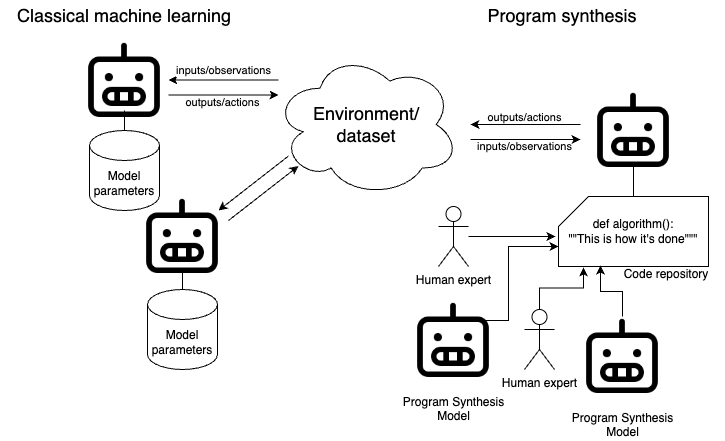
\includegraphics[width=\linewidth]{mlvsautocode.png}
    \caption{Program synthesis allows for knowledge sharing}
    \label{fig:mlvsautocode}
\end{figure}

The search in a space of possible programmatic solutions to a problem can be initialized with an existing program that has been developed by an expert in the field (perhaps with the  use of AI tools), thus \textcolor{accent}{importing existing knowledge} from previous efforts of solving the same problem.
This process is not dissimilar to what is known in deep learning as \emph{fine-tuning}: initializing the optimization process of model parameters with a model already trained on a similar task, but it has the additional advantage that the initial code can be generated by a model of a completely different architecture or by a human.

After the search process has been concluded, all of the knowledge incorporated into the resulting system can be \textcolor{accent}{examined and verified}. 
Unlike the black-box model, the approach makes it trivial to answer questions like "Does this model include factor X in its decision-making on topic Y?".
This offers us an additional way of verifying the decision system before its final deployment. 
And, unlike the numerous post-hoc methods of machine learning interpretability \cite{linardatosExplainableAiReview2020}, this approach involves a strong guarantee that the explanation does not diverge from the behavior.

Of course, the external observers of a program synthesis system can be not only teachers, but also students. 
Even if the resulting program is never deployed, one can read it and \textcolor{accent}{export the knowledge} and incorporate it into future systems, as well as textbooks and other didactic materials for humans.

\newpage
\section{Broader impacts}
\label{sec:impacts}

\epigraph{The Future's So Bright, \\ I Gotta Wear Shades}{Timbuk 3}

\paragraph{Capability}

The \emph{expressivity and peformance} of programming languages can lead to \emph{decision support systems}, also known as \emph{digital assistants}, that are more capable, better able to make predictions and provide advice.

The ability to \emph{import, verify and export knowledge} into or out of a decision suport system can reduce or even eliminate the amount of \emph{knowledge silos} that exists in the ecosystem of these agents, where each separate system has been trained on some data set of its own and some expert knowledge of its own and each incorporates some small part of existing knowledge about the field. 

Insufficient capability in digital assistants can be a major safety risk, especially when they're deployed fully autonomously. For example, misidentification of obstacles in autonomous driving \cite{sheebajoiceObstacleDetectionSafe2023} or wrongful diagnosis in healthcare \cite{wintersDiagnosticErrorsIntensive2012} can be a matter of life and death.

\paragraph{Alignment}

Highly capable digital assistants present their own family of safety risks. 
If perverse incentives are present in the optimization goals of the decision system, then a highly capable decision system can bring about harmful situations intentionally.
Most optimization targets are imperfect proxies of intended outcomes. 
An optimization process can thus \emph{game} (\emph{hack}) the metrics and achieve negative outcomes, despite technically improving the metrics.
Common types of \emph{reward hacking} \cite{skalseDefiningCharacterizingReward2022} include:
\begin{description}
    \item[reward tampering] \cite{everittRewardTamperingProblems2021, skalseInvariancePolicyOptimisation2023} - acting on the reward mechanism directly, i.e. disabling sensors involved in performance evaluation or writing more flattering documentation.
    \item[adverse selection] - selectively solving subtasks that are easier to solve even if they happen to be more important.
\end{description}

To give a real world example, both phenomenons have been observed in Healthcare: \cite{shenSelectionIncentivesPerformance2003} find that incentives can lead to the most severely ill patients being less likely to receive care. \cite{fairbrotherImpactFinancialIncentives2001, ImpactPhysicianBonuses, roskiImpactFinancialIncentives2003} find that metrics are sometimes improved by better documenting the incentivized results, not improving them.
\cite{longFairnessMachineLearning2021} notes how misguided fairness metrics incentivize decision systems to intentionally harm people from healthier demographic groups in order to advance equality of outcomes ("equity").

These issues are present in society \cite{nestianPerverseIncentiveGeneral2017} with or without artificial intelligence, they are studied in economics under the umbrella of the \emph{principal agent problem} \cite{pandaAgencyTheoryReview2017}. 
However, powerful optimization algorithms have potential to exacerbate those issues \cite{hadfield-menellIncompleteContractingAI2019}. 
And while the first line of defense is, of course, improving the incentives, one can be skeptical as to whether the incentives can ever represent their designers' intentions perfectly.

In fact, the instrumental convergence theory \cite{benson-tilsenFormalizingConvergentInstrumental} posits that perverse incentives are inherent to any reinforcement learning context, because optimizing for any goal can be aided by increasing the amount of control over one's environment the agent has, and thus any optimization of agents creates incentives to maximize their own power and control. 
First introduced in science fiction \cite{clarke2001SpaceOdyssey2016, ellisonHaveNoMouth1967, jonesColossus2019}, this is now an active area of technical research \cite{jiAIAlignmentComprehensive2024}.
Estimates of the potential dangers of misaligned artificial intelligence range from non-trivial to existential \cite{mcleanRisksAssociatedArtificial2023}.

The interpretability afforded by the program synthesis approach provides a second line of defense against perverse incentives, namely examining the control program and trying to establish whether any of the modules in that program are attempting to game the optimization metrics, manually or with the use of AI tools.

\begin{figure}[H]
    \centering
    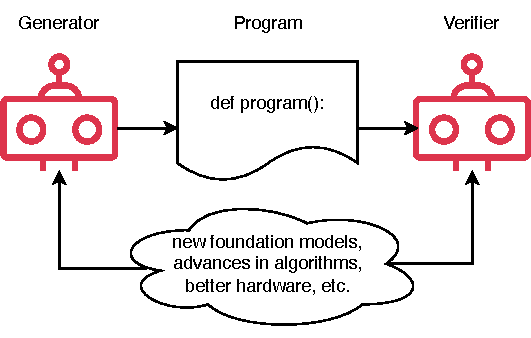
\includegraphics{PSAlign.drawio}
    \caption{Program Synthesis as an alignment methodology}
    \label{fig:ps-as-alignment}
\end{figure}

As the field of artificial intelligence advances, this advances both the generative tools and the verification tools, thus making program synthesis a viable approach to scalable oversight \cite[section 5]{amodeiConcreteProblemsAI2016}.

\paragraph{Human-Robot Teams}

Transparency is a foremost principle of effective teamwork: every member of the team is supposed to know what and why every other member is doing. 
This principle is supported by the study of human teams \cite{bagPeerTransparencyTeams2012, solomonInferenceTransparencyEffective2021} and human-robot teams \cite{ezenyilimbaImpactTransparencyExplanations2022, guznovRobotTransparencyTeam2019, holderDesigningBiDirectionalTransparency2021, lakhmaniExploringEffectCommunication2019, lakhmaniProposedApproachDetermining2016, mercadoIntelligentAgentTransparency2016, ososkyDeterminantsSystemTransparency2014, panganibanTransparencyAutonomousTeammates2020, ronconeTransparentRoleAssignment2017} alike.
Some literature in Human-Robot teams takes inspiration \cite{shivelyCrewResourceManagement2018} from teamwork research in aviation where studies into the common causes of incidents and accidents \cite{chidesterPersonalityFactorsFlight1990, chidesterPilotPersonalityCrew1991, smithSimulatorStudyInteraction1979} have been used to formulate core principles of Crew Resource Management, such as "Verbalize Verify Monitor".
And as more automation is introduced in aviation, the modern cockpit itself can be seen as a human robot team.
Same is true of an operating theater with a robot assistant \cite{weerarathnaHumanRobotCollaborationHealthcare2023} or a doctor using a clinical decision support system \cite{castilloConsiderationsSuccessfulClinical2013, mooreIntroductionClinicalDecision2011, osullivanDecisionTimeClinical2014, purcellWhatMakesGood2005, sakallarisClinicalDecisionSupport2000, selfClinicalDecisionSupport2008, stangeThisIssueClinical2011, wrightClinicalDecisionSupport2009}

The lack of transparency is an important roadblock for integration of black box decision systems in safety critical domains: when conflict arises between the opinion of the expert and the opinion of the system, a black box system offers no additional information for the resolution of the conflict. 
A program, on the other hand, offers the experts a way to explicitly examine why a certain advice is given and use this information to take or not take the advice into account. 
Consequently, a black box system can only be used to completely replace a certain job - any setting where a collaboration is required between a human and decision system requires some degree of transparency that can be afforded by technology like program synthesis. 
This ensures synergistic decision-making where the analysis of every participant is taken into account of the final decision.

\paragraph{Compliance}

Both individual organizations and regulatory authorities often impose requirements onto decision systems that are impossible to effectively enforce without transparency. 
An audit has to be able to establish whether the system violates discrimination law \cite{hochDiscriminationSakeFairness2024, schererApplyingOldRules2019}, accounting standards \cite{julischComplianceDesignBridging2011} or clinical norms \cite{flodgrenExternalInspectionCompliance}.
These requirements are a major impediment to deployment of machine learning in regulated safety-critical domains such as aviation \cite{torensGuidelinesRegulatoryFramework2021, vidotQualificationAvionicSoftware2024} and healthcare \cite{granlundRegulatoryCompliantMLOpsOravizio2021}.
A program, on the other hand, can be audited and proven to be compliant. 
Program synthesis can bring all the advantages of big data-driven systems into such fields without necessitating a regulatory reform.
These concerns become increasingly relevant as explainability of intelligent systems evolves from an implicit legal incentive \cite{hackerExplainableAIContract2020} to an explicit requirement \cite{linardatosExplainableAiReview2020}.

\paragraph{Privacy}

The ineffiency of inference of current machine learning models is (along with competitive pressures) a core reason of the "cloudification" of artificial intelligence: as of late 2023, the most powerful products of machine learning \cite{achiamGpt4TechnicalReport2023} are distributed as remote services that can be interacted with, but not fully copied, via the Internet.
Asking a state of the art decision support system for advice means sending the (potentially sensitive) request to the model provider and making both requests and responses known to said provider \cite{PrivacyPolicy}.
Programs, in contrast, are easier to distribute and performant enough to run on most devices most of the time.
The advent of program synthesis can pave the way to more privacy-preserving decision support: even if the generative model remains in the cloud, one can first use the model to synthesize the program, download it and then submit the sensitive data to the program locally.

\paragraph{Scientific discovery}

Lastly, export of knowledge out of a automatic programming system can be a powerful tool of scientific discovery. 
Symbolic regression is already widely used in physics in order to find formulas that fit experimental results \cite{angelisArtificialIntelligencePhysical2023, tenachiDeepSymbolicRegression2023}. 
In fact, it is not unreasonable to claim that physics \emph{is} a set of symbolic regression problems \cite{udrescuAIFeynmanPhysicsinspired2020}, historically solved manually, but increasingly with some application of algorithms. 
The same can be said about biology \cite{chenRevealingComplexEcological2019}, economics \cite{claveriaAssessmentEffectFinancial2017, lianModelingForecastingPassenger2018, panInfluentialFactorsCarbon2019, truscottDetectingShadowEconomy2011, truscottExplainingUnemploymentRates2014, yamashitaCustomizedPredictionAttendance2022} or any field that develops formulas based on series of empirical observations.

%----------------------------------------------------------------------------------------

\newpage
\chapter{For Personal Healthcare}
\section{Program Synthesis in Healthcare}

Healthcare is a domain where the advantages of program synthesis (as introduced in section \ref{sec:impacts}) are particularly relevant.
\begin{itemize}
    \item Decision systems in Healthcare have a very high threshold for their \emph{capabilities} as patient's health and life can be at stake and mistakes are particularly harmful.
    \item No less dangerous is the risk of perverse incentives and insufficient \emph{alignment} of decision systems with the interests of the patient.
    \item Due to the risks above, decision systems in Healthcare are never deployed fully autonomously. Instead, they have to support doctors in making the final decisions and have to be \emph{good team-players}, explaining the rationale behind every suggestion and supporting dialogue.
    \item Healthcare is a highly regulated domain and \emph{compliance by design} is a crucial feature of any decision systems deployed therein
    \item \emph{Privacy} of clinical data is of utmost importance.
    \item Novel \emph{scientific discoveries} in healthcare have a particularly positive social impact.
\end{itemize}

This is especially relevant as healthcare systems struggle with understaffing \cite{ashleyy.metcalfHospitalUnitUnderstaffing2016,SurveyShowsHidden1993,UnderstaffingSignificantIssue2012,campbell_universal_2013, hudsonUnderstaffing2015, mercerMessageEditorinChief2008, r.stanleyUnderstaffedOverwhelmed2010, munnUnderstaffingWardsCompromising2017, thelancetHealthcareSystemStaffing2018}. Automation tools that make use of Machine Learning (also known as Healthcare 4.0 \cite{tortorellaHealthcareTrendsChallenges2020}) have been consistently identified as crucial for reducing the workload of Healthcare professionals and improving the quality of care \cite{agrawalMachineLearningHealthcare2020, deviDesignImplementationAdvanced2022, g.kumarSurveyMachineLearning2016, ganguliMachineLearningPursuit2020, maityMachineLearningImproved2017, mitraMachineLearningHealthcare2021, pianykhImprovingHealthcareOperations2020, xhaferraRoleMachineLearning2022}.

\begin{figure}
    \centering
    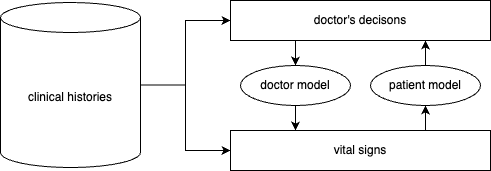
\includegraphics[width=0.8\linewidth]{images/PatientModeling.drawio.png}
    \caption{Modeling in Healthcare}
    \label{fig:modelhealth}
\end{figure}

\begin{figure}
    \centering
    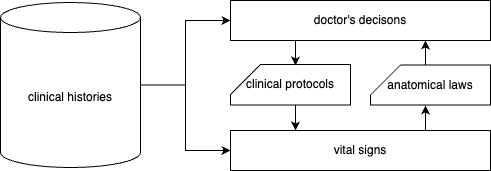
\includegraphics[width=0.8\linewidth]{images/PatientModelingInter.drawio.png}
    \caption{Interpretable Modeling in Healthcare}
    \label{fig:modelhealthinter}
\end{figure}

\begin{figure}
    \centering
    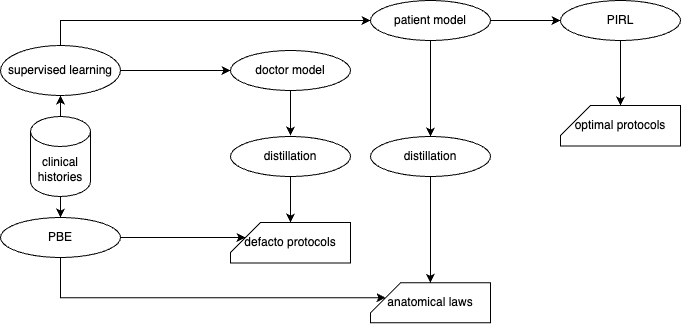
\includegraphics[width=\linewidth]{images/PSHealth.drawio.png}
    \caption{Program Synthesis in Healthcare}
    \label{fig:pshealth}
\end{figure}




\newpage
\section{Patient Simulators as Benchmarks}
\citeself{section}{liventsevEffectivePatientSimulators2021}

Benchmarks orient AI \cite{liangHolisticEvaluationLanguage2022}. Whether it's ImageNet \cite{dengImagenetLargescaleHierarchical2009} in Computer Vision or GLUE \cite{wangGLUEMultitaskBenchmark2018} in natural language processing, benchmarks are a core research tool in mature applications of machine learning, enabling quantitative analysis of learning methodologies to guide and orient their development.
Machine learning in Healthcare, an emergent field with unique challenges in availability of research datasets \cite{Anshik2021Handling, Gilbert2015market, Pahwa2021Big, Yazhini2019State} lacks an accepted benchmarking standard: recent literature reviews \cite{palMachineLearningHealthcare2023,tortorellaHealthcareTrendsChallenges2020} of the field cover a variety of studies that each use their own (often non-public) benchmark. The shortage of standard benchmarks has been consistently identified as a central roadblock for machine learning in Healthcare
\cite{Crown2015Potential, David2020Evaluating, guSupervisedLearningPervasive2023, harutyunyanMultitaskLearningBenchmarking2019, Kathrin2022Benchmark, liventsevEffectivePatientSimulators2021, mcdermottReproducibilityMachineLearning2021, purushothamBenchmarkingDeepLearning2018, S2017Benchmark}.

\newpage
\section{Auto-ALS}
\label{sec:virtu-als}

\citeself{section}{liventsevEffectivePatientSimulators2021}

\begin{figure}
    \centering
    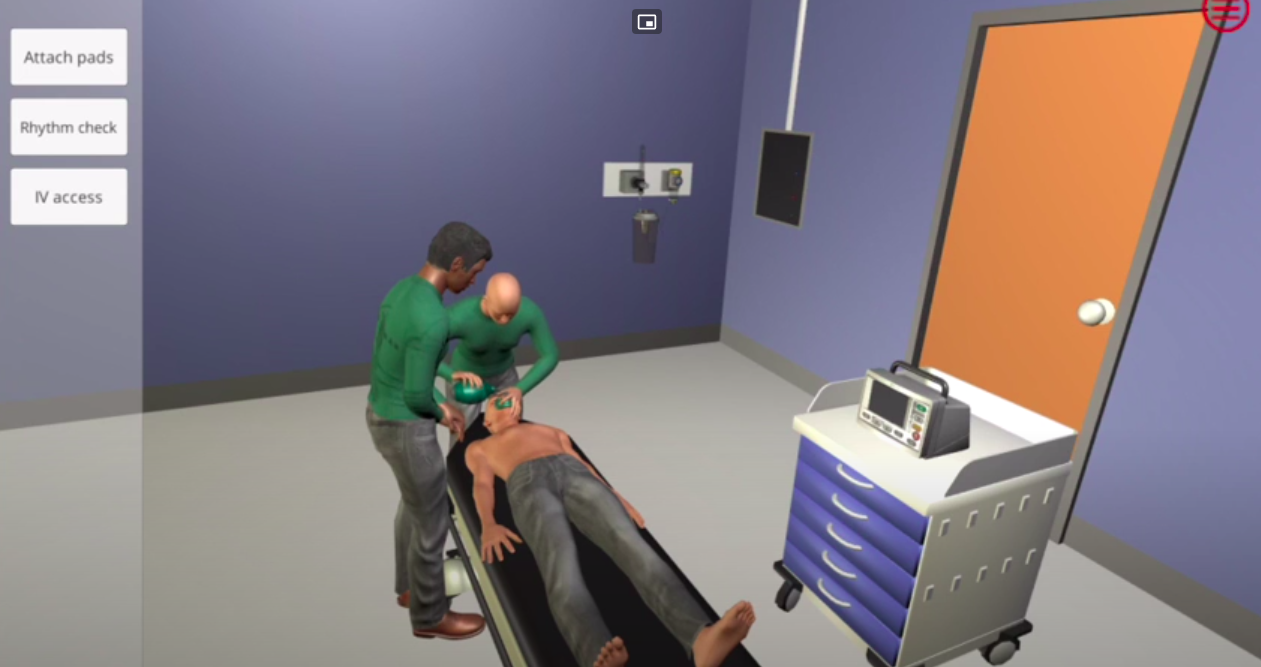
\includegraphics[width=\linewidth]{Virtu-ALS.png}
    \caption{Virtu-ALS}
    \label{fig:virtu-als}
\end{figure}

Virtu-ALS is a \emph{didactic} emergency care simulator mainly targeted at students and junior healthcare professionals, although its application as a reinforcement learning \emph{benchmark} was anticipated and accounted for by the authors \cite{briskAIEnhanceInteractive2018}.
Its most prominent feature is its visual nature (figure \ref{fig:virtu-als}): the user has access to a 3D-rendered virtual copy of a hospital room, view the monitor, press buttons on a defibrillator, etc.
However, the visual modality means that its observation space 
\begin{equation}
    \mathcal{O} \subset R^{307200}
\end{equation}

Such a high dimensionality of the observation space makes it an extremely challenging reinforcement learning task.
Tasks from this family have been solved with deep neural networks \cite{mnihPlayingAtariDeep2013}, however not only does it require a long and expensive training process, it also means that resulting treatment strategies are black box neural networks that no clinical expert understands.
This approach to decision making is extremely hard to introduce into clinical practice \cite{priceBigDataBlackbox2018,watsonClinicalApplicationsMachine2019}

Like most \emph{didactic} simulators, Virtu-ALS exhibits considerable \emph{confirmation bias} - any decision that's not supported by the standard emergency care protocol \cite{thimInitialAssessmentTreatment2012} is considered a mistake and rewarded negatively.

As our first model, we propose a low-dimensional version of \emph{Virtu-ALS}.
\emph{Auto-ALS} is a modification of Virtu-ALS that removes all the complexity of dealing with a visual 3D environment while retaining all the complexity of dealing with a patient that requires emergency care.
This is achieved by attaching an event listener to Virtu-ALS that registers all observable events that can occur in the simulator in response to the user's actions.
The events are listed in table \ref{tab:auto-als}, organized by which agent action can trigger which event.
\emph{Tick} is a special event that occurs every time the simulator is advanced a timestep, and is negatively reinforced, which when used with reinforcement learning algorithms discourages clinicaly unnecessary actions.

\begin{equation}
     o^{+} = \langle \rlobs_1 \in \rlobs_1, \exp(t_1-t), \dots, \rlobs_n \in \rlobs_n, \exp(t_n-t), \rangle
\end{equation}

where $\rlobs_i$ is the value of the observation and $t$ is current time and $t_i$ is time when observation $i$ (for $i=5$, \verb|ResponseGroan|) has \emph{last} occurred and $\exp(t_i-t)$ represents its decaying relevance.
For \emph{measurements}, the $\rlobs_i$ equals the magnitude of the measurement, however, for binary obsevations $\rlobs_i$ would always be equal to one.
For memory efficiency, for all $i$ that correspond to binary observations, $\rlobs_i$ is skipped from the $o^{+} $ vector and the actual observation vector $o$ has size $36+7*2=50$, as opposed to $36+7)*2=86$

\newpage
\subsection{Decision process}
\label{sec:mpdp}

Implementing Auto-ALS requires grappling with some of the limitations of POMDP framework (as described in section \ref{sec:taxonomy})
\begin{enumerate}
    \item Some decision making scenarios legitimately have a discrete flow of time: a CPU, for example, makes a decision every $\frac{1}{\text{clock frequency, Hz}}$ of a second. However, most real-life decision making settings (such as the hospital setting) happen in a continuous time flow with no limits on how often or how rare actions and observations occur.
    \item The agent cannot respond to an observation with less than one (i.e.~zero) or more than one action. This can be fixed by modeling $\rlaction_n)$ as a set of actions.
\end{enumerate}

Both of these problems have been successfully addresed with artificial time discretization and complex action spaces $\rlactions$, however this is done on a case by case basis for each particular environment. A general model that addresses these challenges would be very useful.

\paragraph{Message Passing Decision Process}

(working title, alternatives include the simpler but
\href{https://homes.cs.washington.edu/~todorov/courses/amath579/reading/Continuous.pdf}{somewhat
already taken} \emph{Continuous Decision Process}, the software-jargony
\emph{Event Loop Decision Process} and the insufferably vane
\emph{Liventsev Decision Process})

Let us attach a timestamp $t$ to every observation, reward and action in the decision process, making them 2-tuples. An action $\langle a, t\rangle$ is a message from the agent to the environment, an observation $\langle \rlobs, t \rangle$ or a reward $\langle r, t \rangle$ is a message from the environment
to the agent. Messages can be sent as often or as rare as needed:

\begin{figure}
\centering
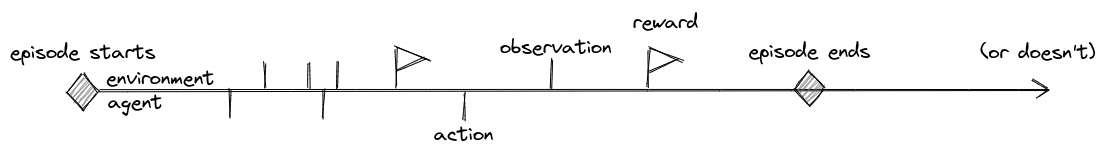
\includegraphics[width=\linewidth]{images/mpdp.png}
\caption{Message Passing Decision Process}
\end{figure}

Observations and actions are sampled from the \emph{environment} and
conditioned on the timestamp and all actions of the agent before that
time:

\begin{equation}
    \rlobs_t \sim p(\rlobs_t|t,\{\rlaction, t_\rlaction | t_\rlaction < t\})
\end{equation}

The actions are sampled from the \emph{agent}, also conditioned on the
timestamp and all observations before that time:

\begin{equation}
a_t \sim \pi(a_t|t, \{ o, t_o | t_o < t \})
\end{equation}

where $\rlobs_t \in O\^{}\{+\}$
and $a_t \in A\^{}\{+\}$

\begin{equation}
    O\^{}\{+\} = \{\text{no observation} \} \cup O 
\end{equation}

\begin{equation} 
A\^{}\{+\} = \{\text{noaction} \} \cup A 
\end{equation}

\paragraph{Discretization}

Now that we're done with the theory, it is a good time to remember that
we live in the real world and, in the real world, unless you plan to run
reinforcement learning algorithms on a
\href{https://royalsocietypublishing.org/doi/10.1098/rstb.2018.0372}{liquid
computer} (in which case, please let us know how it goes!), evaluation
of $\pi(a_t)$ will be done
either by a regular computer that can only evaluate it a finite number
of times a second or something even slower than that. Hence,
discretization is still desirable. However, we need a discretization
strategy that will make the resulting discrete decision process
equivalent (or at least as equivalent as possible) to the continuous
MPDP.

\paragraph{Decision schedules}

So we've established that the practicalities of implementing a
reinforcement learning algorithm mean that in any timeframe
$\langle t, t + \Delta t \rangle$ a finite number of decisions should
be taken. This can be achieved by a decision schedule that is some
combination of:

\begin{itemize}
\item
  making a decision every time any message from the environment
  (observation or reward) is received
\item
  making a decision at regular intervals
  $\Delta t$
\item
  after making a decision, scheduling a decision time
  $t_d$ later in the future
\end{itemize}

At every decision point the agent has to receive information about the
observations that recently occured and output some number of actions
(may be zero)

\paragraph{Observation space}

When an observation is modeled as $\langle \rlobs, t \rangle$, the most faithful way to represent the history of observations to the agent is

\begin{equation} 
\overrightarrow{\rlobs} = \langle \rlobs_1, t_1, \rlobs_2, t_2, \dots \rangle 
\end{equation}

This representation has 2 issues: 
\begin{enumerate}
    \item It has a variable size. There are, of course, \href{https://www.bioinf.jku.at/publications/older/2604.pdf}{machine
learning algorithms that can work with variable size inputs}, however,
most traditional RL approaches cannot and compatibility with them would
be an advantage
    \item There is a common type of observation that makes older
observations obsolete. For example, in a thermostat a new temperature measurement for all intents and purposes overrides the old one. In a navigation task, a new "location observed" event means you are no longer in the previous location. In Auto-ALS, new measurement of a vital sign, such as heart rate, overrides earlier ones. This has to be taken into account, lest a vast array of outdated information will be fed to the agent at every decision point.
\end{enumerate}

A solution (probably \emph{the} solution?) to these is to sort observations into \emph{observation classes} $\rlobs_1 \cup \rlobs_2 \cup \dots
\cup \rlobs_n = O$ such that if several observations from the same class has been made, only the last of them is important. Then $\overrightarrow\{o\}$ should
be a vector of the latest observation in each class

\begin{equation} \overrightarrow\{o\} =
\langle \rlobs_1 \in \rlobs_1,
\exp(t_1-t), \dots, \rlobs_n \in
\rlobs_n, \exp(t_n-t), \rangle
\end{equation}

where $t$ is the decision time.
$\exp(t_n-t)$ is preferable
to the more naive approach of $t-t_n$,
because if no observation in the observation class
$\rlobs_n$ has occurred yet,
$t=-\infty$ which creates all
kinds of problems for actually solving the MDP downstream.
$\exp(t_n-t)$ in this case
would be simply zero and observations that have occured will have an
exponentially decaying relevance factor attached to them - a more
directly useful value for decision-making then ``time since event''.

\paragraph{Action space}

Using one of the decision schedules and the observation system described above, it is fairly trivial to support a variable number of actions. 
The agent has to output an action $\rlaction \in \rlactions$ and if that action is not a "no action", action sampling repeats again.

\newpage
\subsection{Observations}
\label{sec:auto-als-obs}

\texttt{MeasuredHeartRate, MeasuredRespRate, MeasuredCapillaryGlucose, MeasuredTemperature, MeasuredMAP, MeasuredSats, MeasuredResps} are \emph{measurements}, events that have a value $\-infty; +\infty)$ associated with them.

    
The events in table \ref{tab:auto-als} only get registered if the agent has \emph{learnt} some piece of information, meaning that, for example, \verb|AirwayVomit| will only occur if the patient has vomit in their airway \emph{and} the agent checked the airway (which is part of the standard protocol \cite{abcde}).
Assessment skills (knowing where to look and how to establish the patient's state) are crucial for patient resuscitation, hence revealing all known health variables to the agent would jeopardize the simulation.

The observation vector in \emph{Auto-ALS} is based on all observations that have occurred between the beginning of the episode and current time.
However, more recent observations are more likely to still be relevant and should be given priority.
This is done with the following formula proposed in section \ref{sec:mpdp}:

\begin{equation}
     o^{+} = \langle \rlobs_1 \in \rlobss_1, \exp(t_1-t), \dots, \rlobs_n \in \rlobss_n, \exp(t_n-t), \rangle
\end{equation}

\newpage
\subsection{Actions}
\label{sec:auto-als-act}

\begin{table}[H]
\begin{tabular}{|p{0.4\linewidth}|p{0.45\linewidth}|c|}
\toprule
Agent actions &
  Patient reactions & Rewards
   \\
   \midrule
AssessResponse &
  ResponseVerbal,     ResponseGroan,     ResponseNone &
  \multirow{9}{*}{0} \\
AssessAirway &
  AirwayClear,     AirwayVomit,     AirwayBlood,     AirwayTongue &
   \\
AssessBreathing &
  BreathingNone,     BreathingSnoring,     BreathingSeeSaw,     BreathingEqualChestExpansion,     BreathingBibasalCrepitations,     BreathingWheeze,     BreathingCoarseCrepitationsAtBase,     BreathingPneumothoraxSymptoms,  VentilationResistance, \emph{MeasuredRespRate} &
   \\
AssessCirculation &
  RadialPulsePalpable,     RadialPulseNonPalpable, \emph{MeasuredHeartRate} &
   \\
AssessDisability &
  \verb|AVPU_A|,     \verb|AVPU_U|,     \verb|AVPU_V|, PupilsPinpoint,     PupilsNormal, \emph{MeasuredCapillaryGlucose} &
   \\
AssessExposure &
  ExposureRash,     ExposurePeripherallyShutdown,     ExposureStainedUnderwear, \emph{MeasuredTemperature} &
   \\
AssessDefibrillator &
   &
   \\
AssessMonitor &
  HeartRhythmNSR,
    HeartRhythmSVT,
    HeartRhythmAF,
    HeartRhythmAtrialFlutter,
    HeartRhythmVT,
    HeartRhythmMobitzI,
    HeartRhythmMobitzII,
    HeartRhythmCompleteHeartBlock,
    HeartRhythmTorsades,
    HeartRhythmBigeminy,
    HeartRhythmVF, \emph{MeasuredHeartRate}, \emph{MeasuredMAP}, \emph{MeasuredSats}, \emph{MeasuredResps} &
   \\
   DoNothing & & \\
   \midrule
ABG,     AirwayManoeuvres,     GiveAtropine,     GiveAdenosine,     GiveAdrenaline,     GiveAmiodarone,     GiveMidazolam,     Venflon,     Yankeur,     DrawBloods,     BPCuffOn,     BVM,     Guedel,     NRBMask,     DefibOn,     DefibAttachPads ,     DefibShock,     DefibCharge ,     DefibChangePaceCurrentDown,     DefibChangePaceCurrent,     DefibEnergyDown,     DefibEnergyUp,     DefibChangePaceRateDown,     DefibChangePaceRateUp,     DefibPace& 
   Blunder & $r_\text{blunder}$
   \\
   \midrule
   \multirow{2}{*}{Finish} & Failure & -1 \\
   & Success & 1 \\
   \midrule
   - & Tick & $r_\text{tick}$ \\
  \bottomrule
\end{tabular}
\caption{All actions and observations of Auto-ALS}
\label{tab:auto-als}
\end{table}


\newpage
\chapter{The State of the Art}\label{ch:autocode-sota}
Automatic program synthesis has been a long term goal of the field of artificial intelligence since its inception \cite{mannaAutomaticProgramSynthesis1971}, promising to reduce the workload of software developers by automatically solving some of the tasks they face.
And since the field's inception it has been grappling with the challenging properties of the sparse optimization space \cite{alurSyntaxguidedSynthesis2013, davidProgramSynthesisChallenges2017} that is the set of all programs in a certain programming language, namely, 
\begin{enumerate}
    \item valid error-free programs constitute an exceedingly small part of the space of possible strings, so any program synthesis algorithm that incorporates random guessing (for instance, Reinforcement Learning with random initialization \cite{suttonReinforcementLearningSecond2018}) is exceedingly unlikely to guess a valid program;
    \item a small edit in a program can result in a large difference in it's behavior (and, conversely, the same algorithm can be expressed with very different programs), hence the programs we would like to find are not clustered in any compact part of the optimization space;
    \item some of the evaluation mechanisms of programs, especially in the \emph{Programmatically Interpretable Reinforcement Learning} paradigm involve stochasticity and can yield different results for the same program.
\end{enumerate}

In other words, the search space in program synthesis is \emph{sparse}, \emph{brittle} and sometimes \emph{noisy} \cite{arnoldNoisyOptimizationEvolution2002} - all known challenges in Optimization Theory.
Methods of program synthesis can be classified by how they address these challenges.

\newpage
\section{Genetic programming}
\label{sec:gp}

\begin{figure}[H]
    \centering
    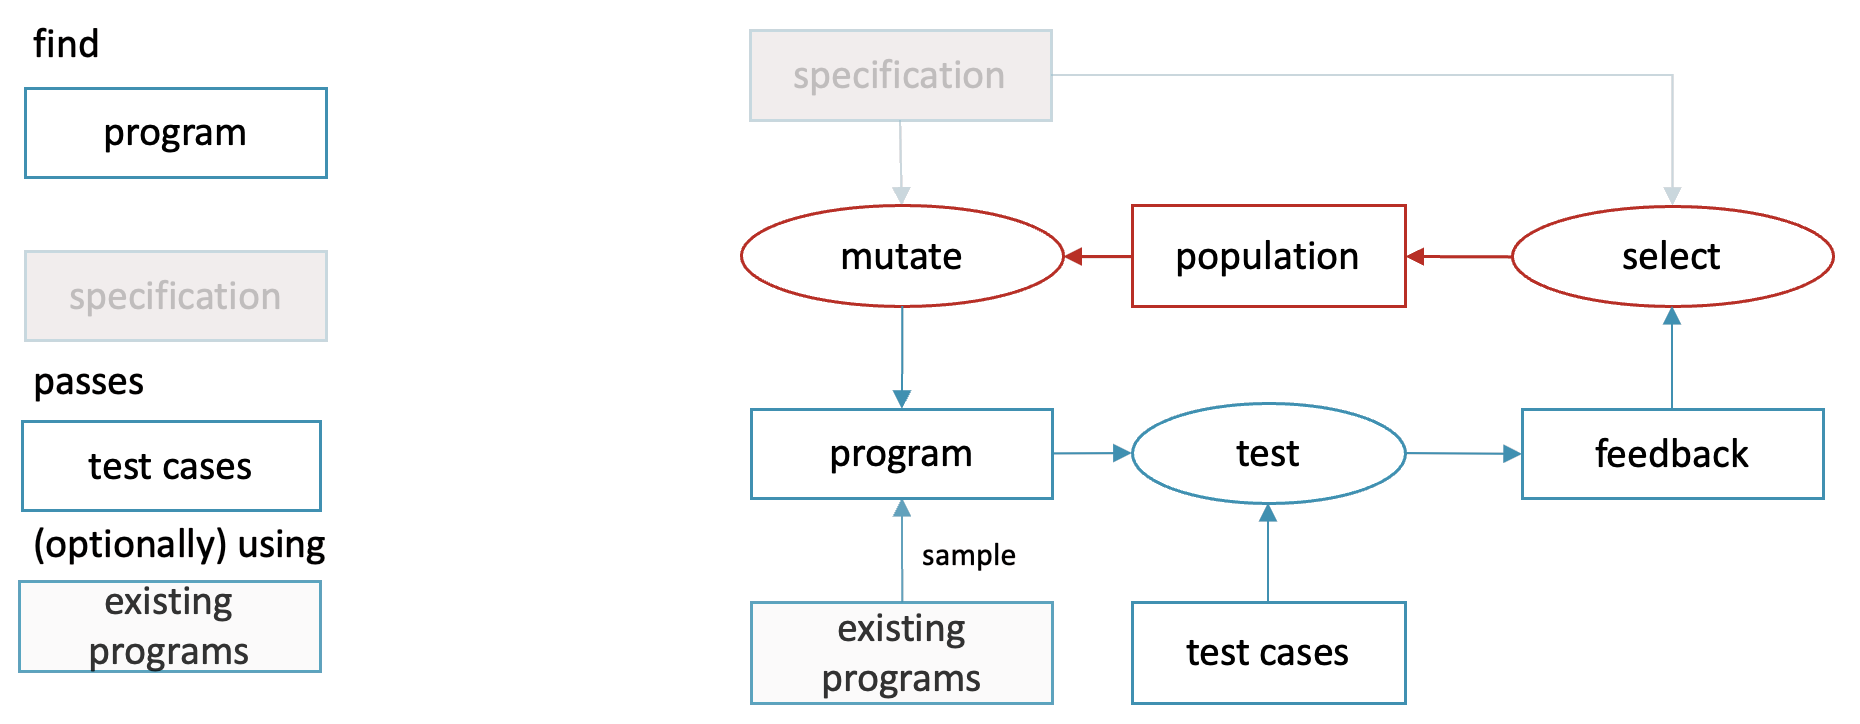
\includegraphics[width=\linewidth]{gp.png}
    \caption{Genetic Programming, schematic definition}
    \label{fig:gp}
\end{figure}

The family of optimization methods best applicable to this type of complex non-differentiable search space is \emph{genetic and evolutionary methods} - biologically inspired methods that operate on a population of candidate solutions (programs), randomly edit (\emph{mutation}) and combine (\emph{recombination}) to expand the population and the prune the population by \emph{natural selection}: removing the candidates that adhere to the specification the least.
Within program synthesis this family of methods is known as \emph{genetic programming} \cite{genprog1, genprog2, genprogast}
In an evolutionary setting, as soon as at least one (preferably several) valid program is found, initializing the population to include them drastically speeds up the search process, thus addressing the sparsity issue.
This approach is particularly powerful in a setting where some solutions are already known, but a program synthesis system can be used to search for solutions that fit the \emph{specification} even better, a setting known as \emph{genetic improvement of software} \cite{petke2018:genetic}.

Genetic programming has been successfully applied in various domains, including prediction and control \cite{dracopoulosGeneticProgrammingPrediction1997}, the synthesis of complex structures \cite{kozaHumancompetitiveApplicationsGenetic2003}, and the evolution of neural network modules \cite{degarisGENETICPROGRAMMING1990}. In the field of engineering, genetic programming has been applied to systems modeling, control, optimization, scheduling, design, and signal processing \cite{willisGeneticProgrammingIntroduction1997}. 

The biggest drawback of GP is that it requires generation and evaluation of a very high number of programs: higher than most other methods (see chapter \ref{ch:seidr}).
If evaluation of a generated program is computationally expensive, this translates directly into a very high computational cost of program synthesis.

\newpage
\section{Constrained programming languages}
\label{sec:constrainedpl}

Another way to address the complexity of the search space is to select a programming language such that the space of possible programs in that programming language exhibits less of the undesirable properties of optimization spaces.
For examples, a language where any combination of valid characters is a valid program \cite{brainfuck} eliminates a significant share of the complexity of the problem.
This family of approaches is explored in more detail in chapter \ref{ch:bfpp}, including  introduction of a novel constrained programming language for \emph{programmatically interpretable reinforcement learning}

\paragraph{Domain specific languages}

In some application domains it is common to express algorithms in domain specific programming languages \cite{fowlerDomainspecificLanguages2010, hudakDomainspecificLanguages1997, karsaiDesignGuidelinesDomain2014, kosarComparingGeneralpurposeDomainspecific2010, kosarDomainspecificLanguagesSystematic2016, mernikWhenHowDevelop2005} that tend to be more limited in terms of token vocabulary and grammatical complexity.
This provides the program synthesis community with a natural experiment in constraining the complexity of a language to simplify (automatic or manual) programming.
As a result, some of the most notable early positive results were in an industry standard database query language (SQL \cite{groffSQLCompleteReference2002}) \cite{liCanLlmAlready2024, yuSpiderLargescaleHumanlabeled2018} and an educational 2D robot control language (Karel \cite{pattisKarelRobotGentle1994}) \cite{metainduction}.

\paragraph{Logic programming}

One domain that's particularly amenable to solving synthesis tasks is \emph{logic programming}: a programming paradigm based on formal logic \cite{doetsLogicLogicProgramming1994, lloydFoundationsLogicProgramming2012}. 
In contrast to other programming paradigms \cite{floydParadigmsProgramming2007, gorodniaiaStudyProgrammingParadigms2016, krishnamurthi13ProgrammingParadigms2019, vanroyProgrammingParadigmsDummies2009} all functions in logic programming languages are boolean, which drastically limits the space of possible functions and makes many search-based approaches possible.

\todo{Deductive}

\todo{Inductive}

%Instead of (or in addition to) generating a program first and testing whether it adheres to specification, \emph{deductive} methods apply equivalence rules to translate the specification into an executable.
%This is hard to apply in \emph{programmatically interpretable reinforcement learning} where the specification is a black box, but can be a powerful approach in \emph{code translation} and \emph{programming by example} paradigms.


\newpage
\section{Unsupervised pre-training}
\label{sec:pretrain}

The paradigm of foundation models \cite{foundation-models} has recently been very prominent in machine learning and machine learning on source code is no exception.
In this paradigm, a model is first trained on a large dataset to solve a generic task such as next-token prediction and then used as a central component in solutions of various specific tasks.


\paragraph{Autoregressive models}

% Why this approach
Most modern foundation models are \emph{autoregressive}, i.e. trained to predict the a token in a program given all the preceding tokens.
This paradigm makes it easy to collect training data and parallelize computation.

% Architectures
\todo{Some words on architectures}

% Models
Autoregressive foundation models for source code, based on architectures such as GPT Codex \cite{radfordImprovingLanguageUnderstanding,chenEvaluatingLargeLanguage2021,codegen,gpt-neo} and BERT \cite{devlinBERTPretrainingDeep2019,codebert} have enabled significant process in tasks like programming by example \cite{halbertProgrammingExample1984} and even human-comparable performance in coding competitions \cite{liCompetitionLevelCodeGeneration2022}.

\paragraph{Autoencoder models}

While undoubtedly useful in many program synthesis tasks, popular foundation models may fall short in the areas of genetic programming \cite{genprogast} and genetic improvement of software \cite{petke2018:genetic}.
In these settings, new programs are found by exploring the space of programs similar to one or several reference programs.
The task of applying these perturbations to programs could benefit from a foundational model, however, it's unclear how to achieve this with the current autoregressive models.
Autoencoder Genetic Programming \cite{autoenc-gp,denoising-autoenc-gp,latentspaceopt} argues for using autoencoder \cite{autoencoders} models instead.
These models embed programs into a high-dimensional vector space, making it easy to mutate a program by add random noise to the embedding vector or combine several programs by averaging their embedding vectors.
Autoencoder-genetic programming is discussed in detail in chapter \ref{ch:tree2tree}.

\newpage
\section{Grammar guided synthesis}
\label{sec:grammar-guided}

Another way to constrain the hypothesis space is to use the grammar of the programming language in question directly in the program generation process.
Since in most implementations of compilers and interpreters, the first step of program execution is building an Abstract Syntax Tree representation of the code a software tool for AST parsing is available for most programming languages.

\begin{figure}[H]
    \centering
    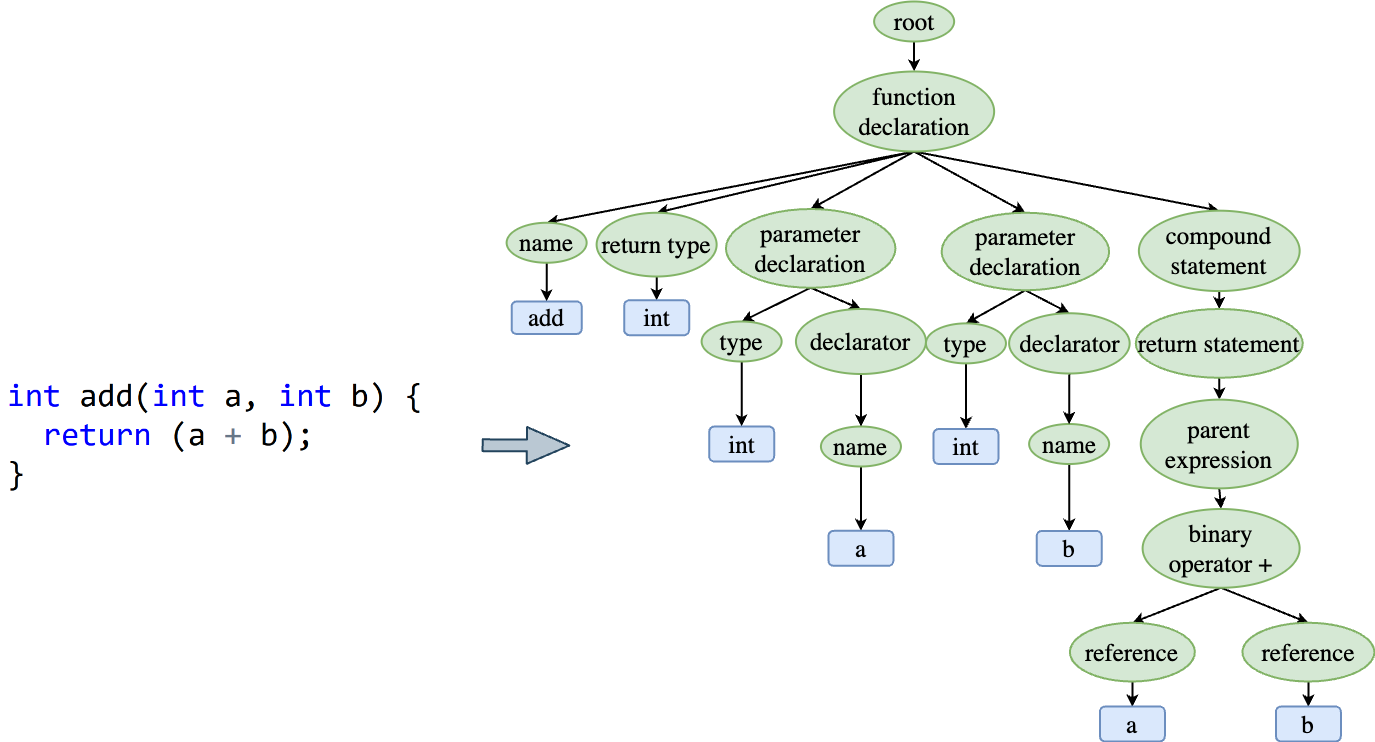
\includegraphics[width=\linewidth]{images/ast.png}
    \caption{Abstract syntax tree (AST) parser}
    \label{fig:ast-parser}
\end{figure}

When program synthesis systems  output ASTs, as opposed to raw text, a large class of errors (such as forgetting a semicolon) becomes impossible. 
Research literature on structural code encoding \cite{alon2019structural,zhang2015tree}, structural code decoding \cite{jiang2021ast,zhu2019grammarcnn} and grammar-guided genetic programming \cite{bunelLeveragingGrammarReinforcement2018, manriqueGrammarguidedGeneticProgramming2009, sobaniaChallengesProgramSynthesis2020a} suggests that models that operate directly on the tree structure of the program can achieve better performance than models that operate on a sequence of tokens.

A hybrid solution, combining an unstructured pretrained language model with inference-time grammar guidance is \emph{constrained decoding} \cite{melcerConstrainedDecodingCode2024}: an algorithm based on excluding tokens disallowed by the grammar of the programming language when sampling tokens from a model.

A novel approach to grammar guided program synthesis is proposed in chapter \ref{ch:tree2tree}

\newpage
\section{Human in the loop}
\label{sec:human}

Alternatively, one can narrow the scope of the problem by retaining a human developer in the loop, but supporting them with CASE \cite{caseComputeraidedSoftwareEngineering1985} tools that solve some of the subtasks involved in developing a program.

\paragraph{Parametrization}

Differentiable programming \cite{blondelElementsDifferentiableProgramming2024} involves programming languages designed such that if a program computes function $f(x)$ the compiler can compute a derivative $f'(x)$. 
With differentiable programming machine learning can be used to adjust all constants defined by the human developer.

Probabilistic programming \cite{gordonProbabilisticProgramming2014} is a programming paradigm where the developer is allowed to specify non-deterministic branching so that which pathway gets executed is decided randomly or externally.
The probabilities of different branches can be uniform or they can be learned in a \emph{programming by example} or \emph{programmatically interpretable reinforcement learning} fashion.
As a result, human developer outlines the options for behavior of the system at every stage and then machine learning computes which options are better suited to the data at hand.

\todo{TerpreT}

\paragraph{Sketch completion}

The paradigm of program synthesis by sketching predates large language models for code \cite{solar-lezamaProgramSynthesisSketching2008} and involves a human developer writing an approximate sketch of the desired program and a program synthesis system fills in the gaps and adds the missing details.

Today, this can be done with a \emph{programming copilot}: a software tool integrated into the text editor as a core feature or an extension, that used a pretrained language model to recommend code snippets based on the context (the code already present in the file).
At first glance \emph{copilots} may seem like a tool to accelerate typing, however, the developer can also imitate the "natural language to machine language" paradigm by describing the task at hand in a comment (or function name or docstring) and letting the copilot solve the task.

\begin{figure}[H]
    \centering
    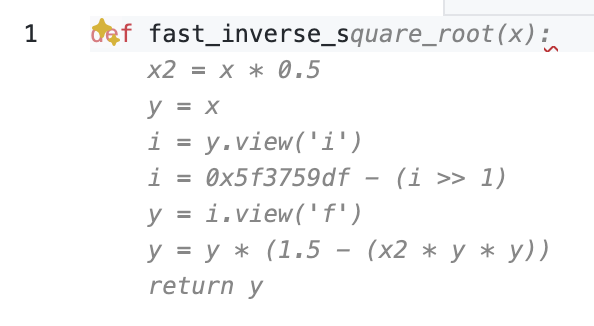
\includegraphics{images/fastinversesqrt.png}
    \caption{Github Copilot \cite{dakhelGithubCopilotAi2023, nguyenEmpiricalEvaluationGitHub2022, wermelingerUsingGithubCopilot2023} suggests an efficient algorithm for calculating inverse square root \cite{lomontFastInverseSquare2003} before the developer has finished typing the name of the method}
    \label{fig:fastinversesqrt}
\end{figure}

According to a large-scale survey \cite{liangLargeScaleSurveyUsability2024} \todo{what?}

\newpage
\section{Open problem}
\label{sec:goal}

The methods above have led to significant progress in \emph{code translation} and \emph{programming by example}, to the point where these paradigms have current industrial applications.
\emph{Programmatically Interpretable Reinforcement Learning}, however, largely remains an open problem.

\begin{highlight}
The goal of this thesis is to discover a methodology for Programmatically Interpretable Reinforcement Learning that can improve decision support systems in Healthcare and other safety-critical domains.
\end{highlight}


We model the task as {\em Episodic Partially Observable Markov Decision Process}:

\begin{multline}
\langle \rlnontermstates, \rltermstates, \rlactions, \rlobss, \rlobsdistr, \rlstatedistr, \rlrewardf, \rlinitdistr \rangle
\end{multline}

Here, $\rlnontermstates$ is the set of {\em non-terminal (environment) states} and $\rltermstates$ is the set of {\em terminal states}. 
$\rlactions$ is the set of {\em actions} that the learning agent can perform, and $\rlobss$ is the set of {\em observations} about the current state that the agent can make. 

A \emph{reinforcement learning episode} starts in a state $\rlstate \in \rlnontermstates$ sampled from $\rlinitdistr$, the {\em initial distribution} over environment states.
An agent action $\rlaction \in \rlactions$ at the state $\rlstate$ causes the environment state to change probabilistically, and the destination state follows the distribution $\rlstatedistr$. 
At state $\rlstate$, the probability of making observation $\rlobs$ is $\rlobsdistr$ and the probability of obtaining \emph{reward} $\rlreward$ is $\rlrewardf$. 
The process continues until $\rlstatedistr$ yields a terminal state $\rlstate \in \rltermstates$.
This distinction is what sets \emph{episodic} POMDP popularized by OpenAI gym \cite{openai-gym} apart from the more traditional approach \cite{kramerjdavidrPartiallyObservableMarkov1964, spaanPartiallyObservableMarkov2012} where the process is infinite.

A \emph{program} is a sequence of tokens

\begin{equation}
    \code=(\code^{(1)},\code^{(2)},\dots)
\end{equation}

that defines behavior of an agent.
Depending on the programming language and implementation choices the tokens can be characters or higher-level tokens, i.e. keywords.
We denote the language's \emph{alphabet}, i.e. the set of all possible tokens as $\alphabet$.

An \emph{interpreter} is a tuple $\langle \rlactionf,\rlmemoryf \rangle$ where $\rlmemoryf(c_k,m_k,o_k)$ is the \emph{memorization function} that defines how the agent's memory updates upon making an observation and $\rlactionf(c, m_k)$ is the \emph{action function} defines which action the agent at a certain memory state takes in the POMDP.
Memory is intialized at state $\rlmemory_\text{init}$

The agent's goal is maximizing total reward collected in the environment, calculated as follows:

\begin{algorithm}[H]
\begin{algorithmic}[1]
\caption{Evaluating total reward for a program}
\Function{$\mathit{Eval}$}{$\code$}
\State $\rlreturntot \gets 0$
\State $\rlmemory \gets \rlmemory_\text{init}$
\State $\rlstate \sim \rlinitdistr$
\While{$\rlstate \in \rlnontermstates$}
\State $\rlobs \sim \rlobsdistr$
\Comment{Observe}
\State $\rlmemory \gets \rlmemoryf(\code,\rlmemory,\rlobs)$
\State $\rlaction \gets \rlactionf(\code, \rlmemory)$ 
\Comment{Act}
\State $r \sim p_r(s,a)$
\State $R_\text{tot} \gets R_\text{tot} + r$
\Comment{Get rewarded}
\State $\rlstate_\text{next} \sim \rlstatedistr$
\Comment{Next state}
\State $\rlstate\gets s_\text{next}$
\EndWhile
\State \Return $\rlreturntot$
\EndFunction
\end{algorithmic}
\end{algorithm}

Since the algorithm for computing this function involves repeatedly sampling values from distributions, function $\mathit{Eval}(c)$ is a mapping from the set of programs to the set of real-valued random variables.

The \emph{Programmatically Interpretable Reinforcement Learning} objective then becomes

\begin{equation}
    \expectation(\mathit{Eval}(\code)) \longrightarrow \max_{\code}
    \label{eq:pirlgoal}
\end{equation}

The following chapters propose novel solutions to the task above. Chapter \ref{ch:seidrforhealth} applies the best-performing solution to Auto-ALS, the benchmark outlined in section \ref{sec:auto-als}.

\newpage
\chapter{BF++}\label{ch:bfpp}
\chapter{BF++}\label{ch:bfpp}

\citeself{chapter}{liventsev2021:bf}

\section{BF++}
\label{sec:language}

\todo{Cite deceptive diversity}

\paragraph{BF syntax}
\label{sec:bf}

Abolafia {\sl et al} \cite{abolafiaNeuralProgramSynthesis2018} picked BF\footnote{Brainfuck} \cite{brainfuck} as their language for program synthesis for the following reasons:
\begin{itemize}
    \item In industry-grade programming languages like Python or Java program code can contain a very large variety of characters since any of the 143859 Unicode \cite{allenUnicodeStandard2012} characters can be used in string literals. In BF, however, only 8 characters can be used: they can be one-hot-encoded with vectors of size 8. 
    \item BF's simple syntax means that an arbitrary string of valid characters is likely to be a valid program. 
    In more complex languages, most possible strings result in a syntax error. 
    A generative model being trained to write programs in such a language risks being stuck in a long exploration phase when all the programs it generates are invalid and it has no positive examples in the dataset.
    \item Despite all of the above, it is a Turing-complete language.
\end{itemize}

The simplicity of the language also means that it is relatively easy to develop a compiler that translates programs from an industry-standard programming languages like Java and Python to BF thus making use of the expert knowledge existing in those languages. 

In the current chapter, we introduce an extended version of the original BF language, BF++. As explained below, the extensions to the original BF syntax are particularly useful in the RL use cases. 

BF's runtime model is inspired by the classic Turing Machine \cite{turing}: at any point during the program's execution, the state of the program consists of:

\begin{itemize}
    \item An infinite\footnote{If one happens to be executing a BF program on a computer with finite memory, the tape will be finite due to hardware limitations.} tape of cells $T$ where each cell holds an integer number.
    \item A \textit{memory pointer} $p_T$ that points to a certain cell in the tape (\textit{active cell} $T^{p_T}$).
    \item A string of characters $C$ that represents program code.
    \item A \textit{code pointer} $p_C$ pointing to a character about to be executed.
\end{itemize}

The code pointer starts at the first character, then this character gets executed and the pointer is incremented (moved to the next character).
There are 8 possible characters:

\begin{description}
\item[\texttt{>}] Move the memory pointer one cell right. $p_T := p_T + 1$
\item[\texttt{<}] Move the memory pointer one cell left. $p_T := p_T - 1$
\item[\texttt{+}] Increment the \textit{active cell}. $T^{p_T} := T^{p_T} + 1$
\item[\texttt{-}] Decrement the \textit{active cell}. $T^{p_T} := T^{p_T} - 1$
\item[\texttt{.}] Write $T^{p_T}$ from the \textit{active cell} to the \textit{output stream}\footnote{The definition of input and output streams is purposefully underspecified, it may depend on the particular implementation.}
\item[\texttt{,}] Read $x$ from the \textit{input stream} to the \textit{active cell}. $T^{p_T} := x$
\item[ \texttt{[} ] If the \textit{active cell} $T^{p_T} = 0$, jump (move $p_C$) to the matching $]$.
\item[ \texttt{]} ] If the \textit{active cell} $T^{p_T} \neq 0$, jump (move $p_C$) to the matching $[$
\end{description}

[ and ] commands constitute a loop that will be executed repeatedly until the \textit{active cell} becomes zero.
They are also the only way to write a BF program with a syntax error: a valid BF program is one that does not contain non-matching [ or ].

% TODO: example?

\paragraph{Negative values}

In \textbf{BF} memory cells $T^i$ hold non-negative values only.
In \textbf{BF++} $T^i \in \mathbb{Z}$, a negation operator \texttt{\~} is introduced and operators \texttt{[]}are redefined to loop while the \textit{active cell} is non-positive, i.e.

\begin{description}
\item[ \texttt{\~} ] If the \textit{active cell} $T^{p_T} := - T^{p_T}$.
\item[ \texttt{[} ] If the \textit{active cell} $T^{p_T} \geq 0$, jump (move $p_C$) to the matching $]$.
\item[ \texttt{]} ] If the \textit{active cell} $T^{p_T} < 0$, jump (move $p_C$) to the matching $[$
\end{description}

This decision was taken because negative observations are common in control problems (see section \ref{sec:bfpp-experiments}) as is branching on whether the observed value is positive or negative. 

\paragraph{Non-blocking action operators}
\label{sec:queue}

% TODO: cite some literature
% We're not the first people tackling these challenges, right?

The main issue of \textbf{BF} as a language for Reinforcement Learning is its input-output system.
It assumes that the program can freely decide on the relative frequency of inputs to outputs.
For example, the following program

\begin{center}
\begin{lstlisting}
+[.....,]
\end{lstlisting}
\end{center}

inputs 5 integers, outputs the 5th character it read, then goes back to the beginning and proceeds indefinitely outputting every 5th character it inputs.
Thus it assumes a 5:1 frequency of inputs to outputs.
If we simply assume that inputs are observations and outputs are actions, such program will not be able to operate in a POMDP environment where I/O frequency is fixed at 1:1 and the agent that has made an observation has to act before it can make the next observation.
In other words, operators \texttt{.} and \texttt{,} are blocking: \texttt{.} stops program execution and waits until new input is received to resume execution, \texttt{,} stops program execution and waits until there is an opportunity to act in the environment.

To address this, in \textbf{BF++} \texttt{.} operator is non-blocking.
It outputs the current value of the active cell by placing it at the bottom of the \textit{action queue} $S$ - a sequence of integer numbers that represent actions the program is planning to take in the environment. We also introduce a non-blocking operator \texttt{!} that places $T^{p_T}$ on top of the action queue.

\begin{equation}
    \begin{array}{cc}
         . & S := S^\frown (T^{p_T}) \\
         ! & S := (T^{p_T})^\frown S
    \end{array}
\end{equation}

where $\frown$ denotes concatenation of tuples

The program can thus decide by using \texttt{.} or \texttt{!} whether the newly added action takes precedence over ones already in the queue.
As soon as an opportunity to act arises, the top of the action queue (item $S^1$ or several items $S^1,S^2,\dots$, see section \ref{sec:envs}) defines which action the program takes and is then removed from the queue. 
If $S^k$ does not exist (the queue is empty or shorter than $k$) default value of $S^k=0$ is assumed.

\texttt{,} operator, on the other hand, is blocking. 
Thus its function is more important than just reading an observation into memory.
Executing \texttt{,} is when the program moves to the next step of POMDP.

\paragraph{Virtual comma}
\label{sec:virtualcomma}

% TODO: fading text for virtual commas

The system where the only way to proceed to the following iteration is the \texttt{,} operator, naively implemented, means that to be successful in any POMDP environment, a program has to contain an infinite loop with a \texttt{,} operator.
Any program that has a finite number of \texttt{,} steps will terminate prematurely in an environment that supports arbitrarily long number of iterations.
Since the original goal is to develop a language where most random programs would be valid, this had to be addressed.

We decided to turn any \textbf{BF++} program into an infinite loop with a \texttt{,} operator by default:
\begin{enumerate}
    \item Every \textbf{BF++} program starts with a virtual \texttt{,} operator at address $p_C = -1$: it is executed before all operators in the code of the program, they are indexed starting from $p_C = 0$
    \item When the code pointer $p_C$ reaches the end of the program it loops back to the virtual comma $p_C := -1$
\end{enumerate}

Due to the virtual comma, every program starts executing with the initial observation already stored in memory and available for branching/decision-making.

\paragraph{Observation discretization}
\label{sec:observe}

Another issue complicating applications of \textbf{BF} to Reinforcement Learning is that since its memory tape holds only integer numbers its inputs and outputs have to be integers as well.
And this issue cannot be fixed simply by replacing an integer tape with a tape of floating point numbers as \textbf{BF}'s only operations for manipulating numbers are \texttt{+} and \texttt{-} - increment and decrement.
Non-integer action and observation spaces are fairly common in reinforcement learning tasks hence \textbf{BF++} implements coercion mechanisms for reading and writing continuous vectors into discrete memory.

We assume that the vector observation space $O$ is an intersection of $n$ separate scalar observation spaces $O^k$ such that 
\begin{equation}
 o_1 \in O_1^k,o_2 \in O_2^k,\dots,o_n \in O_n^k \Leftrightarrow (o_1,o_2,\dots,o_n) \in O  
\end{equation}

This assumption theoretically excludes some possible observation spaces, but almost all POMDP tasks discussed in the research literature and all Gymnasium tasks conform to this assumption.

To write an observation onto the memory tape we the observation vector of size $n$ is aligned with memory cells $T^{p_T},T^{p_T+1},\dots,T^{p_T+n-1}$ and turned into an integer with the use of $d$ discretization bins.

\begin{equation}
\label{eq:discretization}
T^{p_T+k-1} := \min_{\omega \in 1,\dots d | o^k < \tau^k_\omega} \omega
\end{equation}

If $O^k$ is an interval $O^k=[o_{low}, o_{high}]$, it is split into discretization bins evenly, as in eq. \ref{eq:static-thresholds}:

\begin{equation}
\label{eq:static-thresholds}
\tau_\omega = \begin{cases}
o_{low}+\frac{o_{high}-o_{low}}{d}\omega, \omega=1,2,\dots,d-1 \\
+\infty, \omega=d 
\end{cases}
\end{equation}

\begin{figure}[htb]
    \centering
    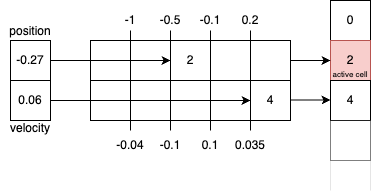
\includegraphics[width=0.8\linewidth]{observ.png}
    \caption{Fluid discretization example in Mountain Car}
    \label{fig:obs}
\end{figure}

Some environments, however, have unbounded observation spaces $O^k=(-\infty;+\infty)$, $O^k=(-\infty;o_{high}]$,  $O^k=[o_{low};+\infty)$.
This spaces are challenging because the formal description $O^k$ does not in any way reflect the actual underlying distributions of observations.
It can be the case, for example, that $O^k=(-\infty;+\infty)$ but most observations found in the environment fall in the interval $O^k=[42;43]$.
For such observation spaces, \textbf{BF++} uses a \textit{fluid discretization} system that learns the true distribution of observations online. The idea was inspired by a work of Touati {\sl et al} \cite{adaptivediscretization}, although, they assumed that $O^k$ has a finite diameter and did not support unbounded observation spaces.
Initial thresholds $\tau_\omega$ can be arbitrary.
With each new observation, thresholds $\tau_\omega$ are readjusted so that among $h$ prior observations, roughly $\omega$ out of $d$  observations are lower values that $\tau_\omega$:

\begin{equation}
\underset{\tau}{\text{minimize}} \sum_{\omega \in 0,1,\dots d} |\frac{\omega}{d} - \frac{\sum_{i' \in i-h,i-h+1,\dots,i-1} \mathbb{I}(o_{i'}^k < \tau_\omega)}{h}|
\end{equation}

To solve this optimization problem, one has to sort previous $d$ observations in ascending order so that 

\begin{equation}
    \text{sort}: \{o_i | i \in i-h,i-h+1,\dots,i-1\} \longrightarrow \{ s_i | i \in 1,2,\dots,h \}
\end{equation}

is such a bijection that $s_1 < s_2 < \dots < s_h$ holds and set

\begin{equation}
    \tau_{\omega} = s_{\lceil \frac{\omega}{d} h \rceil}
\end{equation}

See figure \ref{fig:obs} for a visual example.

%TODO: prove

This system has 2 hyperparameters: $d$ and $h$.
With a low $d$ a lot of the information observed form the environment is lost, while when $d$ is in the hunderds the generated programs can become very complex.
$h$ switches between relative and absolute observations.
With a very high $h$, $\omega=0$ means that this observation is one of the lowest that can be observed in this environment, with $h=1$ it means that the observation is lower than the previous one.

High values of $h$ present an additional challenge: how to correctly discretize observation in the first $h$ iterations?
We implemented \textit{burn-in}: before training or evaluation we run $h$ iterations of a random agent (see section \ref{sec:random}) to collect a history of $h$ observations and pick correct thresholds.

\paragraph{Action coercion}
\label{sec:act}

A symmetrical problem arises with actions taken by the agent. 
Memory tape holds integer numbers $T^k \in \mathbb{Z}$ and any value can be pushed onto the action stack.
However, the action that's output to the environment has to belong to a $N$-dimensional action space $A$, an intersection of unidimensional action spaces $A^k$.
The "act" operation thus includes a coercion system and is defined as:

\begin{equation}
\label{eq:act}
\begin{array}{l}
    a^k := \begin{cases}
\frac{S^k}{d-1}, A^k = (- \infty; + \infty) \\
a_{\text{min}} + |\frac{S^k}{d-1} - a_{\text{min}}|, A^k = [a_{\text{min}}; + \infty) \\
a_{\text{max}} - |a_{\text{max}} - \frac{S^k}{d-1}|, A^k = (- \infty; a_{\text{max}}] \\
a_{\text{min}} + \frac{(S^k \bmod d)}{d - 1} * (a_{\text{max}} - a_{\text{min}}), A^k = [a_{\text{min}}; a_{\text{max}}] \\
S^k, A^k \subset \mathbb{Z}
\end{cases} \\
    S := (S^{N+1}, S^{N+2}, \dots)
\end{array}
\end{equation}

\paragraph{Goto}
\label{sec:goto}

It is notoriously hard to introduce any kind of branching behavior in \textbf{BF} \cite{linanderControlFlowBrainfuck2016}.
To facilitate if-then style programs we introduce a \textit{goto} operator \verb|^| defined as 

\begin{equation}
   p_T := T^{p_T} 
\end{equation}

Note that it is not a \texttt{goto;} in the traditional C sense, since the memory pointer is being moved, not the code pointer.
Still, it lets the agent preemptively store potential actions in memory cells and than branch between this actions based on the observation.

\paragraph{Random number generator}
\label{sec:random}

Operator \texttt{@} writes a random number into the \textit{active cell}.
A random agent is often used as a starting point for exploration and in \textbf{BF++} a random agent can be implemented as \verb|@!|

\paragraph{Shorthands}
\label{sec:shorthands}

With all the commands we introduced in sections \ref{sec:bf} - \ref{sec:goto} it is still surprisingly hard to encode relatively simple decisions like "add action 5 to the top of the action queue":

\begin{center}
\begin{lstlisting}
[>]+++++!
\end{lstlisting}
\end{center}

This program moves the memory pointer right until it hits a cell that contains zero, increments it five times, and then pushes $T^{p_T}$ to the top of the action queue. It also loses the current value of the memory pointer which might be meaningful. Our experiments have shown that it takes a very long time for the neural model to learn to write this kind of combinations.

To mitigate this issue we introduce \textit{shorthands}: commands \texttt{01234} mean "write the respective number (0,1,2,3 or 4)" into the \textit{cell} and commands \texttt{abcde} mean "move the memory pointer to cell a,b,c,d or e" where cells a,b,c,d and e are the first 5 cells in the memory tape.
We intentionally made the number of \textit{shorthands} equal to discretization constant $d=5$.
Due to our method of discretization of continious action spaces (see sections \ref{sec:observe}, \ref{sec:act}) the program will often encounter situations when it can choose between $d$ different actions and thanks to shorthands taking them can be encoded as \texttt{1!}, \texttt{2!}, \dots

\paragraph{Summary}
\label{sec:summary}

In total (assuming 5 shorthands) \textbf{BF++} has 22 commands:

\begin{center}
\begin{lstlisting}
><^@+~-[].,!01234abcde
\end{lstlisting}
\end{center}

Commands \verb|@^~01234abcde| are considered optional and can be disabled if the task at hand calls for it.
The number of shorthand commands can be increased or decreased.

% Achilles hill
Observation discretization and action coercion techniques built into the language mean that \textbf{BF++} is compatible with any POMDP environment. 
However, in practice, there is one important limitation: the complexity of the program required to operate in an environment is directly proportional to dimensionality of it's action and observation spaces $A$ and $O$. 
If, for example the observation space is 10000-dimensional, once an observation is read onto tape $T$ it takes 9999 \verb|>| operators to reach second to last observation.
Thus, in practice, \textbf{BF++} should be used with low-dimensional POMDPs.

An extension of our methodology to high-dimensional POMDPs (such as Atari games \cite{atari}, where the observation is a matrix of pixels on simulated game screen) can be achieved by adding a scene encoder neural network that maps the observed image to a low-dimensional vector as proposed in \cite{daqn}.

\newpage
\section{Experimental setup}
\label{sec:bfpp-experiments}

\paragraph{Hypotheses and goals}
\label{sec:exgoals}

\todo{Rewrite to make Aki happy}

Our experiments were designed to test the following hypotheses:

\begin{description}
    \item[$H_1$] \textbf{BF++} can be used in conjunction with a program synthesis algorithm to solve arbitrary reinforcement learning challenges (POMDPs)
    \item[$H_2$] \textbf{BF++} can be used to take a program written by an expert and use program synthesis to automatically improve it
    \item[$H_3$] \textbf{BF++} can be used to generate an interpretable solution to Reinforcement Learning Challenges that experts can learn from
    \item[$H_4$] Optional commands \verb|@^~01234abcde| introduced for convenience make it easier for experts to write programs in \textbf{BF++}
    \item[$H_5$] Optional commands \verb|@^~01234abcde| improve the quality of programs synthesized by neural models
\end{description}

Hence we

\begin{enumerate}
    \item Pick several commonly studied reinforcement learning environments
    \item Employ an expert\footnote{the author fo the present thesis} to write \textbf{BF++} programs to solve them
    \item Develop a program synthesis model following from \cite{abolafiaNeuralProgramSynthesis2018}
    \item Compare the best programs generated by the model with expert programs in terms of program quality
    \item Perform ablation studies: remove some of the optional commands from the language (resulting language is called \textbf{BF+}), remove the expert program from the model's program pool, compare program quality
    \item Perform case studies: analyze programs generated by the model to gain insight into how the model approached the problem
\end{enumerate}

\paragraph{Environments}
\label{sec:envs}
%TODO: add table of action and observation spaces

\begin{figure}[t]
    \centering
    \subfloat[CartPole-v1]{
        \centering
        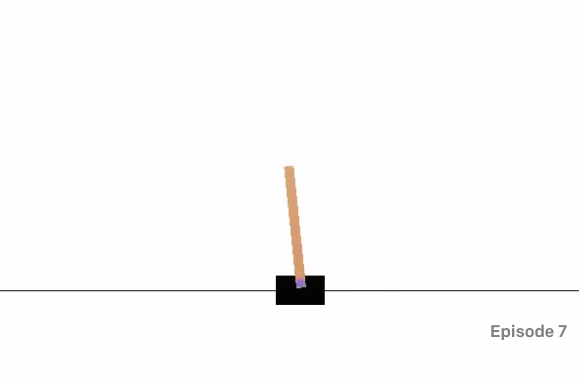
\includegraphics[height=1in]{Cartpole1.png}
    }
    \subfloat[MCC-v0]{
        \centering
        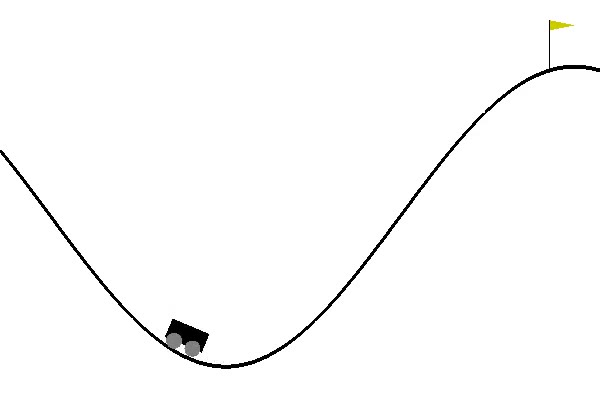
\includegraphics[height=1in]{MountainCar0.jpeg}
    }
    \subfloat[Taxi-v3]{
        \centering
        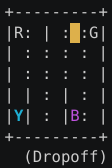
\includegraphics[height=1in]{Taxi3.png}
    }
    \subfloat[BW-v2]{
        \centering
        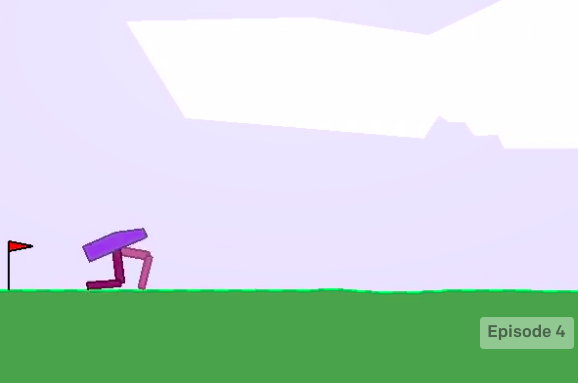
\includegraphics[height=1in]{BipedalWalker2.png}
    }
    \caption{Selected tasks}
    \label{fig:envs}
\end{figure}

We evaluate our framework on 4 low-dimensional (see section \ref{sec:summary}) POMDPs sampled from Gymnasium \cite{towersGymnasiumStandardInterface2024} leaderboard\footnote{\url{https://github.com/openai/gym/wiki/Leaderboard}}:

\begin{enumerate}
\item \textbf{CartPole-v1} \cite{cartpole}.
A pole is attached to a cart.  which moves along a frictionless track.
The agent observes cart position, cart velocity, pole angle and pole velocity at tip.
The goal is to keep the pole upright by applying force between -1 and 1 to the cart.
At every step the agent receives a +1 reward for survival.
The episode terminates when the pole inclines too far.
\item MountainCarContinuous-v0 (\textbf{MCC-v0})\cite{mountain_car}.
A car is on a one-dimensional track, positioned between two "mountains". 
The goal is to drive up the mountain consuming a minimal amount of fuel by controlling the engine, setting it's torque in the range $[-1;1]$; however, the engine is not strong enough to scale the mountain in a single pass.
Therefore, the only way to succeed is to drive back and forth to build up momentum. 
We picked MountainCarContinuous-v0 as opposed to MountainCar-v0 to demonstrate the performance of our discretization system.
\item \textbf{Taxi-v3} \cite{taxi}. There are 4 locations (labeled by different letters) and the goal is to pick up the passenger at one location and drop him off in another in as few timesteps as possible spending as little fuel as possible.
\item BipedalWalker-v2 (\textbf{BW-v2}). A simulated 2D robot with legs has to learn how to walk. 
Moving rightwards is rewarded, falling is penalized.
Observation vector consists of speeds, angular speeds and joint positions collected by the robot's sensors.
These observations do not, however, include any global coordinates - they can only be inferred from sensor inputs.
With action vector of size 4 the agent controls speeds of the robots hip and knee motors.
\end{enumerate}

\paragraph{Hyperparameters}

For observation discretization (section \ref{sec:observe}) we picked $d=5$ (so that it's equal to the number of shorthands) and $h=500$ for our experiments, hence when the observation is among the highest 20\% of the last 500 observations it is written into memory as 4 while if it falls between 40-th and 60-th percentiles it is 2.

\paragraph{Expert programs}
\label{sec:expert-progs}

For \textbf{CartPole} we wrote 2 programs. 
One completely ignores all observations and just alternates between "move right" and "move left":

\begin{center}
\begin{lstlisting}
0!,1!
\end{lstlisting}
\end{center}

Another calculates the difference between velocity of the cart and angular velocity of the pole.
If it's positive, the cart is pushed to the right (the cart has to catch up with the pole), if it's negative the cart is pushed to the left, if zero it is pushed randomly:

\begin{center}
\begin{lstlisting}
[a0>0>0>0>0>@>1>1>1>1>1>,>[->>-<<]>>+++++^!1]
\end{lstlisting}
\end{center}

The first part of this program sets up an action map on the tape where every possible value of the velocity differential has a respective cell with 0, 1 or (in the center) random number.
Then \verb|[->>-<<]| block does subtraction, \verb|+++++| adds 5 to the result, so that it belongs to in $0..10$ and not $-5..5$, \verb|^| moves the memory pointer to the correct cell in the action map and \verb|!| puts the action onto the action stack.

For \textbf{Mountain Car} we wrote an elegant algorithm that reads the observation vector into the tape, goes to the second observation (car velocity) and outputs it as action:

\begin{center}
\begin{lstlisting}
>!a
\end{lstlisting}
\end{center}

In other words, we apply motor torque in the same direction where we're currently headed, thus always accelerating our car.
If we're headed right, that helps us get to the destination and if we're headed left that helps us get as high as possible onto the hill so that when direction reverses, the car has more energy to push through the right hill.

For \textbf{Taxi} we introduce 2 programs.
The first program:
\begin{enumerate}
    \item Finds the coordinates of the current destination (passenger to pick up or current passenger's destination)
    \item Subtracts the current destination 
    \item Moves in the resulting direction
\end{enumerate}

The problem with this approach is that it always gets stuck when it hits a wall.
To compensate for that, the second program alternates between the strategy above (for 5 iterations) and random movements (for 5 iterations) so that it eventually gets unstuck. See source code repository for the programs.

Optional commands \verb|@^~01234abcde| have all been invaluable in developing these programs - a fact in support of $H_4$.
A more rigorous way to confirm it would be employing several human experts to develop programs with and without optional operators, but finding volunteer \textbf{BF++} developers has proven difficult. 

Developing BF++ programs for \textbf{Bipedal Walker} manually is very challenging and left outside the scope.

\paragraph{Program synthesis model}
\todo{ensure standard nomenclature}

In order to train a generative model $g$ to write \textbf{BF++} programs we treat the writing process as a reinforcement learning episode in its own right \cite{abolafiaNeuralProgramSynthesis2018} .
Every character of a program is an action taken by the \emph{writer agent}, the programs are terminated by a NULL character.
When the NULL character is written, a \emph{BF++ agent} is created in the target POMDP environment (e.g. CartPole) and sum total of rewards $Q$ collected in that episode is assigned as a reward to the \emph{writer agent} for the NULL character.
All other characters are rewarded with zero.

The \emph{writer agent's} policy is modeled with an LSTM \cite{hochreiterLongShorttermMemory1997} neural network and is trained with a modified version of REINFORCE \cite{williamsSimpleStatisticalGradientfollowing1992}algorithm.
While standard REINFORCE optimizes Policy Gradient:

\begin{equation}
    O_{\text{PG}}(\phi) = \mathbb{E_{\pi(C; \phi)}}(Q)
\end{equation}

where $\phi$ are LSTM parameters, $C$ - program, $Q$ - reward obtained by the program in target environment,

we optimize

\begin{equation}
    O(\phi)=O_{PG}(\phi)+O_{PQT}(\phi)
\end{equation}

where

\begin{equation}
    O_{\text{PQT}} = \frac{1}{K} \sum_{k=0}^K \log \pi(C_k; \phi)
\end{equation}

where $C_1$ is the best (highest $Q$) known program, $C_2$ - second best, \dots

Intuitively, both $O_{\text{PG}}(\phi)$ and $O_{\text{PQT}}(\phi)$ when optimized update the weights of the LSTM so that programs that we have found to be successful are more likely.
But Policy Gradient weighs programs proportionately to their respective rewards while PQT creates a \textit{priority queue} of the \textit{best known programs} and assigns a high importance to them and zero to the rest.

\begin{figure}
    \centering
    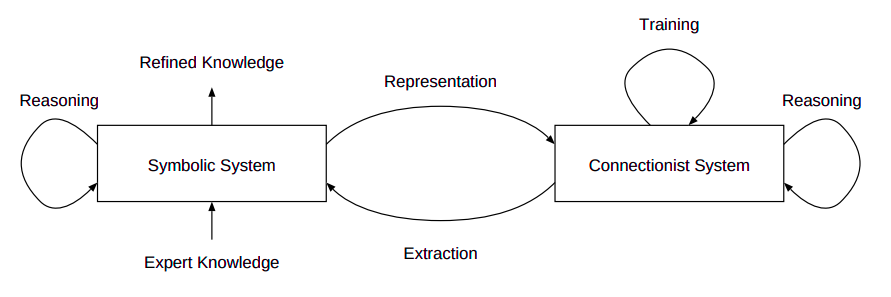
\includegraphics[width=\linewidth]{cycle.png}
    \caption{Neural-symbolic learning cycle \cite{cycle}}
    \label{fig:cycle}
\end{figure}

$O_{\text{PQT}}$ component has been shown to have "a stabilizing affect and helps reduce catastrophic forgetting in the policy" \cite{abolafiaNeuralProgramSynthesis2018}.
In addition to this, we use $O_{\text{PQT}}$ to implement \textbf{expert inspiration}.
By default, the \textit{priority queue} of the \textit{best known programs} is initialized as an empty set.
But if expert-written programs are available, it can be prepopulated with these programs that act as useful positive examples for teaching the \emph{writer agent}.
This approach is used to incorporate programs from section \ref{sec:expert-progs} and transfer knowledge from experts to the neural developer.

This approach to \textbf{expert inspiration} follows what's known as neural-symbolic learning cycle, displayed in figure \ref{fig:cycle} - expert knowledge is represented symbolically, in terms of a \textbf{BF++} program, then a neural network is trained to generate this program, effectively translating the expert knowledge from symbolic into connectionist format (\emph{representation}), the neural network learns from reinforcement how to solve the task better than the expert (\emph{training}).
Unlike in most neural-symbolic systems \cite{neuralsymbolic} that extract knowledge from connectionist systems with algortihms like TREPAN \cite{trepan} or JRip extraction \cite{jripextr}, the \emph{extraction} step is trivial since the neural network outputs a symbolic program directly.

In all experiments below, the \emph{writer agent}'s LSTM has hidden size of 50, batch size of 4 and is trained with RMSProp \cite{tielemanLectureRmsPropDivide2012} optimizer.

\paragraph{Stopping and Scoring}

All experiments were run with an upper limit of 100000 training episodes.
Environments other than \textbf{Taxi} also used Exponential Variance Elimination \cite{evestop} early stopping technique - training was stopped when the postive trend in the quality of the best found program stopped, i.e. when the exponential moving average of program quality is lower that it was 1000 episodes ago.
Agents for \textbf{Taxi} are trained for a fixed number of episodes, because we noticed that in this environment the longest part of the training process is learning to pick up the first passenger and until that happens $Q=-200$ holds.

Once the training process is finished, we take the best known programs and since each of them was only tested once (leading to high variance) we test them again, averaging total rewards over 100 episodes. 
We use this averaged reward to pick the best program.

\paragraph{Implementation}

\textbf{BF++} interpreter and the training system were written in Python with TensorFlow for neural models.
GPU resources were not used, because the performance bottleneck of the system is not backpropagation but rather testing a \textbf{BF++} program in the environment, single experiment runtime was between 1 hour (CartPole) and 10 (Taxi).

\newpage
\section{Results}

\paragraph{Quantitative results}

\begin{table}[H]
  \caption{Total episode reward $Q$ achieved by best programs found, averaged over 100 episodes}
  \label{tab:quality}
  \centering
  \begin{tabular}{lcccc}
    Environment     & CartPole-v1     & MCC-v0 & Taxi-v3 & BW-v2 \\
    \midrule
    Random agent & 9.3 & 0 & -200 & -91.92  \\
    \midrule
    BF++ expert program 1 & 20.48 & -6.55 & -179.49 & - \\
    BF++ expert program 2 & 18.23 & - & -150.44 & - \\
    BF+ (without shorthands) LSTM & 44.55 & 91.57 & -57.93 & -91.9 \\
    BF+ (without \verb|@^~|) LSTM & 48.14 & 81.16 & -42.21 & -31.79 \\
    BF++ LSTM     & 71.38 & 88.41 & -199.82 & -26.97 \\
    BF++ LSTM with expert inspiration  & 96.64 & 91.39 & -60.65 & - \\
    \midrule
    Leaderboard threshold & 195 & 90 & 0 & 300 \\
    \bottomrule
  \end{tabular}
\end{table}

The table above presents the quality metric (average 100-episode reward) of the best program in every category, compared to that of a fully random agent and the result required to join the OpenAI gym leaderboard for context.
Note that the expert programs used a lot of optional operators (shorthands and \verb|@^!|), so it was not possible to implement expert inspiration with limited command sets.

These results support (see section \ref{sec:exgoals}) hypothesis $H_1$ - we have obtained functional programs for all environments, $H_2$ - when expert inspiration was used the resulting programs were better than expert programs and better than programs generated without expert inspiration and $H_4$ - ablation studies for optional operators do indeed show that those operators are useful.

\paragraph{Case studies}
\label{sec:casestudies}
% Need to make sure that this paragraph and "expert programs" paragraph help each other (same style, same terms)

We have established that the program synthesis model is able to learn from human experts.
But can experts learn from the model? ($H_3$) 
To confirm this, we offer a detailed explanation of the most successful program of all experiments listed in section \ref{sec:bfpp-experiments}.

This program scored \emph{91.39} on \textbf{Mountain Car}:

\begin{center}
\begin{lstlisting}
-..~+
\end{lstlisting}
\end{center}

The trailing \verb|~| and \verb|+| do not affect the behavior of the agent: they modify the value of the active cell only for it to be immediately rewritten by the virtual comma (section \ref{sec:virtualcomma}) before it has any chance to influence actions.
One can think about these commands as inactive genes in the DNA - we have found many resulting programs to contain such commands.
If necessary this effect can be accounted for by incorporating program length into the loss function.
So this program is equivalent to:

\begin{center}
\begin{lstlisting}
-..
\end{lstlisting}
\end{center}

\begin{figure}
    \centering
    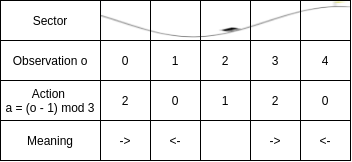
\includegraphics[width=\linewidth]{MountainCarWinner.png}
    \caption{Visual summary of the strategy enacted by \texttt{-..} on \textbf{Mountain Car}}
    \label{fig:mountaincarwinner}
\end{figure}

When the virtual comma is executed, car position and car velocity are read into memory, discretized into integers $0\dots4$.
The position is read into the active memory cell $p_T$, while the velocity is in cell $p_T+1$.
Then the active cell is decremented and the resulting number is put onto the action stack twice.
There is 1 read operation and 2 write operations to the end of the action stack, which introduces a delay before the actions get executed.
When it's time to act, the number on the action stack is coerced to one of the actions possible in this environment (0 for going left, 1 for doing nothing, 2 for right). 

A strategy emerges, illustrated on figure \ref{fig:mountaincarwinner}, in which the car puts "going right" onto the agenda if it's on the far left or the center right of the landscape, puts "going left" onto the agenda when it's on the far right or center left and schedules doing nothing if it's in the center.
This strategy helps the car successfully reach the right fringe every time it is applied.

\newpage
\section{Conclusions}

In this chapter, we have introduced a new programming language tailored to the task of programmatically interpretable reinforcement learning.
We have shown experimentally that this language can facilitate program synthesis as well as knowledge transfer between expert-based systems and data-driven systems. 

The results in the OpenAI gym test examples show that the proposed system is able to find a functional solution to the problem. In some cases the performance is similar to the best deep learning solution but the obtained program remains still explainable. This is a very encouraging result and suggest that the use of program induction methods may indeed be a viable way towards explainable solutions in RL applications. 

We propose the following directions for future work:
\begin{enumerate}
    \item Develop translation mechanisms between \textbf{BF++} and other languages. Potentially, \textbf{BF++} can be used as \emph{bytecode} \cite{bytecode} for reinforcement learning. The expert would write a program in a higher-level language and transpile it into \textbf{BF++} so that the program then can be improved with reinforcement learning.
    \item Use other neural network architectures as well as non-neural evolution methods like genetic programming \cite{genprog1,genprog2} in conjunction with \textbf{BF++}
    \item Apply the framework to problems in Healthcare where expert inspiration is important for crossing the AI chasm \cite{aichasm}.    \item Use Natural Language Generation techniques to translate the BF++ code automatically to a friendly human-readable text description as in \cite{richardsonCode2TextChallengeText2017,code2nlg2}.
\end{enumerate}

\newpage
\chapter{Neurogenetic Programming}\label{ch:neurogen}
\chapter{Neurogenetic Programming}\label{ch:neurogen}
\citeself{chapter}{liventsev2021neurogenetic}

\section{Introduction}\label{sec:neurogen-intro}


In \emph{genetic programming} \cite{genprog1,genprog2} new programs are generated by mutating and mixing a \emph{population} of programs. 
 A more recent approach, largely drawing on the earlier success of deep neural language models (see CodeBERT \cite{codebert} inspired by BERT \cite{devlinBERTPretrainingDeep2019}), have been to train black box \emph{neural models} that generate executable programs as text \cite{abolafiaNeuralProgramSynthesis2018,deepcoder,structural}. 
 Neural program synthesis and genetic programming both have unique advantages \cite{geneticvsneural}. 
 In this chapter we propose a novel hybrid of the two families of methods. We call the method \emph{Instant Scrum} in reference to a popular Agile software team work model \cite{scrum}. We show that \emph{Instant Scrum}, IS, can solve several reinforcement-guided program synthesis tasks in standard OpenAI gym benchmarks tasks (section \ref{sec:tasks}). 

After the introduction to the relevant background in the next section, we will give a detailed description of the proposed IS methodology. Next, we describe the experimental setup and the OpenAI gym test tasks, and the results of the experiments in several variations of the core IS method. Finally, we discuss the results and propose future research directions and potential applications for hybrid neurogenetic programming. 

\newpage
\section{Methodology}

How does one manage a composition of code generators in such a way that the composition yields better programs than individual contributors are capable of? 
This question is studied extensively in software project management literature \cite{mythicalmanmonth}.
And while, admittedly, project management literature is concerned with human developers and, admittedly, there exist considerable differences between human developers and mathematical models of code generation \cite{bugfixing}, we mitigate these differences with several simplifying assumptions.

\subsection{Modeling the codebase}

Following from traditional genetic programming, we define a \emph{population} of programs. 
The \emph{codebase} is a tuple of 2-tuples, representing a program $C_c^{(i)}=c$ and the total reward it collected $C_R^{(i)}=R_\text{tot} \sim \mathit{Eval}(c)$ (see section \ref{sec:quality}):

\begin{equation}
    \mathcal{C} = \langle \langle C_c^{(1)}, C_R^{(1)} \rangle, \langle C_c^{(2)}, C_R^{(2)} \rangle \dots \langle C_c^{(|C|)}, C_R^{(|C|)} \rangle \rangle
\end{equation}

However, unlike in traditional genetic programming, the \emph{initial population} can (optionally) be empty.

\newpage \subsection{Modeling a software developer}
\label{sec:developer}

A software developer can:
\begin{enumerate}
    \item Check out programs from the codebase $\mathcal{C}$
    \item Output new a program $c$
    \item Receive feedback on their program's quality $q$ 
    \item Learn from the feedback by mofidying its strategy
\end{enumerate}

Thus, a developer is a 2-tuple of a program distribution $p_\text{dev}(c | \theta, \mathcal{C})$ and a parameter update procedure $\mathit{Update}(\theta, c, q)$

Distribution $p_{\text{dev}}(c | \theta, \mathcal{C})$ is defined over programs and is parametrized with learnable parameters $\theta$ as well as codebase $\mathcal{C}$. 
Having codebase as parameter enables the developer to generate new programs as a modification and/or combination of existing programs, i.e. to apply genetic programming.

Learnable parameters $\theta$ encode the developer's current methodology of programming that can be modified upon receipt of positive or negative feedback using the developer's update procedure. 

The \emph{team} of developers is a tuple of 2-tuples:
\begin{equation}
    \mathcal{T} = \langle \langle \mathcal{T}_p^{(1)}, \mathcal{T}_\text{upd}^{(1)} \rangle, \langle \mathcal{T}_p^{(2)}, \mathcal{T}_\text{upd}^{(2)} \rangle \dots \langle \mathcal{T}_p^{(|\mathcal{T}|)}, \mathcal{T}_\text{upd}^{(|\mathcal{T}|)} \rangle \rangle
\end{equation}

\newpage \subsection{Modeling program quality}
\label{sec:quality}

We define two empirical metrics of overall program fitness.
The first is \emph{empirical total reward}:

\begin{equation}
    R(c|\mathcal{C}) = \frac{\sum\limits_{i=1}^{|C|} \mathbb{I}[C_c^{(i)}=c] C_R^{(i)}}{\sum\limits_{i=1}^{|C|} \mathbb{I}[C_c^{(i)}=c]}
\end{equation}

If a program has been tested in the environment ($\textit{Eval()}$ function) several times, there will be several copies of it in the codebase with different quality samples.
Averaging over them yields an unbiased estimate of the expectation from equation \ref{eq:pirlgoal}, $\mathbb{E}(\mathit{Eval}(c))$, that we set out to maximize.

The second is \emph{empirical program quality}, defined as

\begin{equation}
    Q(c|\mathcal{C}) = \frac{\sum\limits_{i=1}^{|C|} \mathbb{I}[C_c^{(i)}=c] e^{C_R^{(i)}}}{\sum\limits_{i=1}^{|C|} \mathbb{I}[C_c^{(i)}=c]}
    \label{eq:empquality}
\end{equation}

\emph{Empirical program quality} is an unbiased estimate of $\mathbb{E}(e^{\mathit{Eval}(c)})$
The idea behind exponentiating the total reward is to encourage \emph{exploration} \cite{exploration}.
Programs that on average perform poorly, but sometimes, stochastically, collect high rewards, will have a higher $Q(c|C)$ than $R(c|C)$.
We consider these programs to be \emph{high-quality additions to the codebase} because they contain the knowledge necessary for solving environment $M$, even if on average they do not solve it.
We hypothesize that applying \emph{genetic operators} (section \ref{sec:genetic}) to programs with high $Q(c|C)$ can yield programs with high $R(c|C)$.
For this reason we train developers to maximize $Q$, but when the training is complete, we pick programs from the codebase with the highest $R$ as "best programs".
 
$Q(c|C)$ has an additional technical advantage over $R(c|C)$: invariant $Q(c|C) \geq 0$ holds for all $c$.
This lets one sample programs from the codebase with probabilities proportional to their quality, see eq. \ref{eq:genmixture}.

\newpage \subsection{Populating the codebase}

Just like \emph{instant run-off voting} achieves similar results to \emph{exhaustive ballot runoff voting}, but does it much faster by replacing a series of ballots cast in a series of elections with a ballot cast once that goes on to participate in a series of virtual elections \cite{votingsystems}, our \emph{Instant Scrum} algorithm does the same to Scrum \cite{scrum}: it simulates the iterative software development process recommended by Scrum methodology without humans in the loop making it possible to run many sprints per second:

\begin{algorithm}[H]
\begin{algorithmic}[1]
\caption{Instant Scrum with a team of developers}
\label{alg:instantscrum}
\Procedure{InstantScrum}{$T,\mathcal{C},N_\text{max}$}
\State $N \gets 0$
\While{$N < N_\text{max}$}
\LineComment{For each developer in the team}
\For{$i = 1,2,\dots,|T|$}
\LineComment{Sample a program from the developer}
\State $c_\text{new}\sim p_i(c | \theta_i, \mathcal{C})$ 
\LineComment{Test the program}
\State $R_\text{tot} \gets \mathit{Eval}(c_\text{new})$
\LineComment{Save the code and test result to the codebase}
\State $\mathcal{C} \gets \mathcal{C} \cup \{\langle c_\text{new}, R_\text{tot} \rangle\}$
\LineComment{Train the developer}
\State $\mathit{Update}_i(\theta_i, c, q)$
\LineComment{Increment sprint counter}
\State $N \gets N+1$
\EndFor
\EndWhile
\EndProcedure
\end{algorithmic}
\end{algorithm}

To combine genetic programming and neural program synthesis we introduce 3 types of developers: \emph{genetic} and \emph{neural} and \emph{dummy}, create a team that contains developers of all types and run \emph{Instant Scrum}.

\newpage \subsection{Genetic developers}
\label{sec:genetic}

A genetic developer writes programs by
\begin{enumerate}
    \item Selecting one of the 7 available stochastic \emph{genetic operators} (described below)
    \item Selecting two programs from the \emph{codebase} $C$ (parents $c_1$ and $c_2$) 
    \item Using the operator to modify the parents and yield a new (child) program
\end{enumerate}

A genetic operator is a probability distribution $p_\text{op}$ over child programs given 2 parent programs. 

\begin{equation}
    p_\text{op}(c_\text{child}|c_1,c_2)
\end{equation}

Operators whose $p_\text{op}$ is invariant to $c_2$ and depends on $c_1$ only are called \emph{mutation} operators: they generate a new program by \emph{mutating} one program $c_1$.
The rest are called \emph{combination} operators as they \emph{combine} 2 existing programs to generate a new one.



\paragraph{Mutation operators}

The simplest method for randomly modifying a program is \emph{shuffle mutation}: randomly re-order the tokens of $c_1$.
Let $\mathrm{A}$ be the set of all possible permutations of size $|c_1|$. $|\mathrm{A}|=|c_1|!$. 
Then

\begin{equation}
    p_\text{shuffle}(c_\text{child}|c_1,c_2) =
            \frac{\sum\limits_{\alpha \in \mathrm{A}} \mathbb{I}[\alpha(c_\text{parent}) = c_\text{child}]}{|c_1|!}
\end{equation}

Another approach is \emph{uniform mutation} where a loaded coin is tossed for every token in $c_1$. 
With probability $p_\text{ind}$ it is replaced with a random token from the alphabet $\mathcal{L}$ of the programming language, with probability $1-p_\text{ind}$ it stays the same.
The evolution of a single token under shuffle mutation is defined by distribution

\begin{equation}
    p(c^\text{new} | c^\text{old}) = \frac{p_\text{ind}}{|L|} +  (1 - p_\text{ind}) \mathbb{I}[c^\text{new} = c^\text{old}]
\end{equation}

Hence over full programs the operator is defined as

\begin{equation}
    p_\text{unimut}(c_\text{child}|c_1,c_2) = \mathbb{I}[|c_\text{child}|=|c_1|] \\ 
    \prod\limits_{i=0}^{|c_1|}  \left(\frac{p_\text{ind}}{|L|} +  (1 - p_\text{ind}) \mathbb{I}[c_\text{child}^{(i)} = c_1^{(i)}] \right)
\end{equation}

\paragraph{Combination operators}

The combination operators we propose are all variants of \emph{crossover} - a classic genetic programming technique rooted in the way a pair of DNA molecules exchanges genes during mitosis and meiosis, displayed on figure \ref{fig:crossover}.

In DNA \cite{evocritique}, as well as in most genetic programming literature \cite{genprog1,genprog2} the crossover operator combines 2 parent sequences to produce 2 children.
In this section, in order to reduce complexity, we define the distributions as if only the first child program is saved and the second one is forgotten.
Since program pair $\langle c_2, c_1 \rangle$ is equally likely to be selected for combination as $\langle c_1, c_2 \rangle$ (see eq. \ref{eq:genmixture}) this modification does not affect the resulting genetic developer distribution.

In \emph{one-point crossover} a random cut position $k$ is selected and the trailing sections of 2 parent programs beginning with the cut point are swapped with each other. 
If the parent programs have different lengths, the cut point has to fit within both programs:

\begin{equation}
    2 \leq k \leq |c_1,c_2|; |c_1,c_2| = \min\{|c_1|, |c_2|\}
\end{equation}

Hence the probability of $c_\text{child}$ being born out of \emph{one-point crossover} is

\begin{equation}
    p_\text{1ptcx}(c_\text{child}|c_1,c_2) =
        \frac{\mathbb{I}[|c_\text{child}|=|c_2|]}{|c_1,c_2|-1}
        \sum\limits_{k=2}^{|c_1,c_2|} \prod\limits_{i=1}^{k-1} \mathbb{I}[c_\text{child}^{(i)} = c_1^{(i)}] \prod\limits_{i=k}^{|c_2|} \mathbb{I}[c_\text{child}^{(i)} = c_2^{(i)}]
\end{equation}

\emph{Two-point crossover} is similar, but instead of swapping the trailing ends of programs, a section in the middle of the programs is chosen, determined by randomly selected cut-off indices $k_1$ and $k_2$ and swapped:

\begin{equation}
\begin{split}
    p_\text{2ptcx}(c_\text{child}|c_1,c_2) = // =
        \frac{2 \mathbb{I}[|c_\text{child}|=|c_1|]}{(|c_1,c_2|-2)(|c_1,c_2|-1)}
        \sum\limits_{k_1=2}^{|c_1,c_2|-1}
        \sum\limits_{k_2=k_1+1}^{|c_1,c_2|} \\
        \prod\limits_{i=1}^{k_1-1} \mathbb{I}[c_\text{child}^{(i)} = c_1^{(i)}] \prod\limits_{i=k_1}^{k_2-1} \mathbb{I}[c_\text{child}^{(i)} = c_2^{(i)}]
        \prod\limits_{i=k_2}^{|c_1|} \mathbb{I}[c_\text{child}^{(i)} = c_1^{(i)}]
\end{split}
\end{equation}

\emph{Uniform crossover} mirrors \emph{uniform mutation} in that a loaded coin is tossed for each token in $c_1$. With probability $p_\text{ind}$ the token is replaced, but the replacement is not drawn randomly from the alphabet. Instead, the replacement comes from $c_2$:

\begin{equation}
    p_\text{unicx}(c_\text{child}|c_1,c_2) = \prod\limits_{i=0}^{|c_1|} \mathbb{I}[|c_\text{child}|=|c_1|] \\ \left(p_\text{ind} \mathbb{I}[c_\text{child}^{(i)} = c_2^{(i)}] + (1 - p_\text{ind}) \mathbb{I}[c_\text{child}^{(i)} = c_1^{(i)}] \right)
\end{equation}

Finally, \emph{messy crossover} is a version of \emph{one-point crossover} without the assumption that both parent programs have to be cut at the same index $k$.
In \emph{messy crossover}, one parent is cut at index $k_1$, another is cut at index $k_2$ and the head of one is attached to the tail of the other:

\begin{multline}
    p_\text{messy}(c_\text{child}|c_1,c_2) =
        \frac{1}{(|c_1,c_2|-1)^2}
        \sum\limits_{k_1=2}^{|c_1,c_2|} \sum\limits_{k_2=2}^{|c_1,c_2|} \\ \mathbb{I}[|c_\text{child}|=k_1+|c_2|-k_2] \\ \prod\limits_{i=1}^{k_1-1} \mathbb{I}[c_\text{child}^{(i)} = c_1^{(i)}] \prod\limits_{i=1}^{|c_2|-k_2} \mathbb{I}[c_\text{child}^{(k_1+i)} = c_2^{(k_2+i)}]
\end{multline}

\begin{figure}
    \centering
    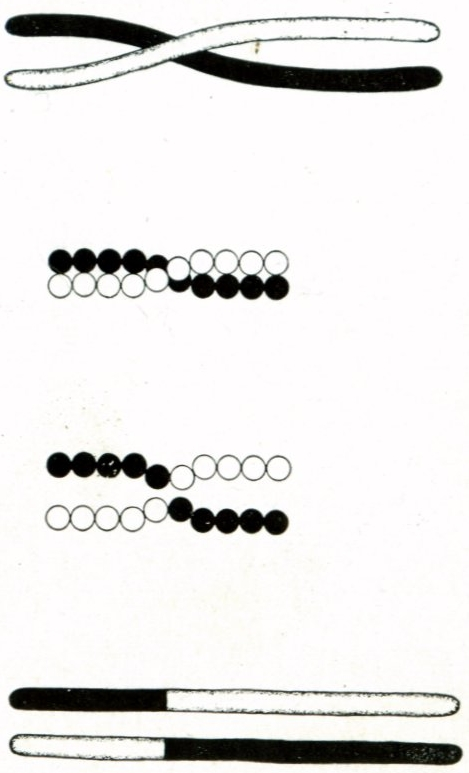
\includegraphics[width=0.45\linewidth]{Morgan_crossover_1.jpg}
    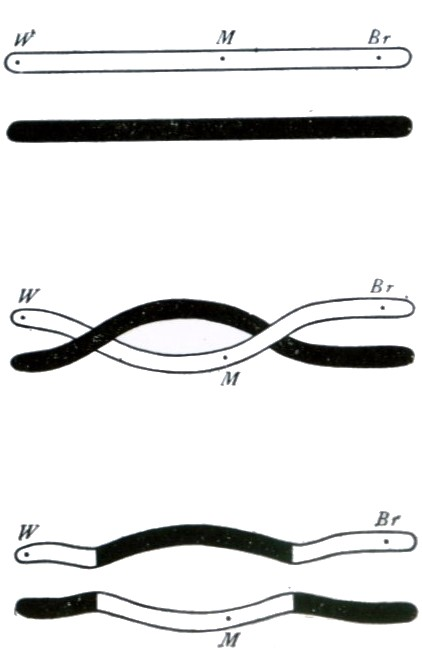
\includegraphics[width=0.5\linewidth]{Morgan_crossover_2.jpg}
    \caption{1-point and 2-point crossover \cite{evocritique}}
    \label{fig:crossover}
\end{figure}

\begin{table}
    \centering
    \begin{tabular}{r|l}
         Parent 1 & \color{blue}\verb|ae>>>>>34+| \\
         Parent 2 & \color{red}\verb|a[e>-a-]b[e>>-b-]| \\
         \midrule
         Shuffle mutation & \color{blue}\verb|>>4+>3>e>a| \\
         Uniform mutation & \color{blue}\verb|ae|\color{black}\verb|@|\color{blue}\verb|>|\color{black}\verb|!|\color{blue}\verb|>>3|\color{black}\verb|5|\color{blue}\verb|+| \\
         1-point crossover & \color{blue}\verb|ae>>>>|\color{red}\verb|-]b[e>>-b-]| \\
         2-point crossover & \color{blue}\verb|ae>|\color{red}\verb|>-a-|\color{blue}\verb|34+| \\
         Uniform crossover & \color{blue}\verb|ae|\color{red}\verb|e|\color{blue}\verb|>|\color{red}\verb|-|\color{blue}\verb|>>3|\color{red}\verb|b|\color{blue}\verb|+| \\
         Messy crossover & \color{blue}\verb|ae>>>>|\color{red}\verb|e>-a-]b[e>>-b-]| \\
         Pruning & \color{blue}\verb|e>>>>>4+| \\
    \end{tabular}
    \caption{All operators applied a pair of BF++ programs}
\end{table}


\paragraph{Pruning operator}

After initial experiments  we found that generated programs often contain sections of unreachable code or code that makes changes to the execution state and fully reverses them.
To address this, we introduced an additional operator for removing dead code (\emph{pruning}): when Instant Scrum encounters a successful program, pruning helps separate sections of this program that led to its success from sections that appeared in a highly-rated program by accident.  

Implementation of the pruning operator depends on the programming language at hand, here we define it as a pruning function $c_\text{pruned}=\mathit{Prune}(c_1)$ that outputs a program functionally equivalent to $c_1$ (memory functions $(\alpha,\mu)$ of $c_\text{pruned}$ are equal to that of $c_1$) and $|c_\text{pruned}| \leq c_1$ and a degenerate probability distribution:

\begin{equation}
    p_\text{prune}(c_\text{child}|c_1,c_2)= \begin{cases}
        1 & c_\text{child} = \mathit{Prune}(c_1) \\
        0 & \text{otherwise}
        \end{cases}
\end{equation}

\paragraph{Operator and parent selection}
\label{sec:selection}

Let $\mathcal{P}_\text{genetic}$ be a tuple of all available genetic operators, in order of introduction, i.e. $\mathcal{P}_\text{genetic}^{(1)}=p_\text{shuffle}$ and $\mathcal{P}_\text{genetic}^{(4)}=p_\text{2ptcx}$

Genetic developer's program distribution is a mixture distribution, combining different operators that can be applied, weighted by learnable parameters, and different programs that can be sampled from the codebase, weighted by \emph{empirical quality} (eq. \ref{eq:empquality}).

\begin{equation}
    p_\text{genetic}(c | \theta, \mathcal{C}) = 
    \sum\limits_{c_1}^{C}  
    \sum\limits_{c_2}^{C} 
    \frac{Q(c_1|C) Q(c_2|C)}{(\sum\limits_{c}^{C} Q(c|C))^2} 
    \sum\limits_{i=0}^{|\mathcal{P}_\text{genetic}|} 
    \theta_i \mathcal{P}_\text{genetic}^{(i)} (c|c_1,c_2)
    \label{eq:genmixture}
\end{equation}

This is a true probability distribution if and only if $\sum\limits_{i=0}^{|\mathcal{P}_\text{genetic}|} 
    \theta_i = 1$


\paragraph{Training the genetic developer}

One challenge that remains to be solved to fully define the genetic developer (folowing section \ref{sec:developer}) is to define a learning from feedback strategy $\mathit{Update}_\text{genetic}$.
To do this, we notice that equation \ref{eq:genmixture} contains a \emph{multi-armed bandit} \cite{banditproblem} hiding in plain sight.
Indeed, once the \emph{genetic} developer samples $c_1$ and $c_2$ from the codebase, it has to pick one of 7 available options (pull one of 7 \emph{levers}) to then receive a reward $\mathit{Eval}(c_\text{child})$.
This subproblem can be represented with a POMDP of its own and solved using one of the standard bandit algorithms \cite{banditsolutions}.

Following \emph{Occam's razor}, we picked the simplest method, \emph{epsilon-greedy optimization}: we calculate the value of each operator as mean total reward of programs generated with this operator:

\begin{equation}
    V^{(i)} = \frac{1}{|\mathcal{C}(\mathcal{P}_\text{genetic}^{(i)})|} 
    \sum\limits_{k=1}^{|\mathcal{C}(\mathcal{P}_\text{genetic}^{(i)})|}
    \mathcal{C}(\mathcal{P}_\text{genetic}^{(i)})_R^{(k)} 
\end{equation}

where $C(\mathcal{P}_\text{genetic}^{(i)})$ is the subset of the codebase produced via operator $\mathcal{P}_\text{genetic}^{(i)}$.

The $\mathit{Update}_\text{genetic}$ procedure recalculates values $V$ and sets operator probabilities to

\begin{equation}
    \theta_i = \frac{\epsilon}{|\mathcal{P}_\text{genetic}^{(i)}|} +
    \mathbb{I}[i = \underset{i}{\arg\max} V^{(i)}] (1 - \epsilon)
\end{equation}

where $\epsilon$ is a hyperparameter responsible for regulating the \emph{exploration-exploitation tradeoff} \cite{banditsexplo}

In future work, however, other bandit optimization algorithms can be used in its place \footnote{Our open-source software implementation allows for drop-in replacement of bandit algorithms}.

\paragraph{Hyperparameters}
\label{sec:genhyper}

The genetic developer, as described above, has 2 hyperparameters:

\begin{enumerate}
    \item $p_\text{ind}$ defines severity of mutation in $p_\text{unimut}$ and $p_\text{unicx}$
    \item $\epsilon$ defines learnability of genetic operator distribution
\end{enumerate}

Note that the \emph{team} mechanism afforded by \emph{Instant Scrum} can be used not only to combine genetic and neural program synthesis, but also to combine several genetic developers with different hyperparameters.

\newpage \subsection{Neural developers}
\label{sec:neural}

The \emph{neural developer}, also known as the \emph{senior developer} because of their unique ability to write original programs, is an LSTM \cite{hochreiterLongShorttermMemory1997} network followed by a linear layer that generates a sequence of vectors $h_{1},h_{2},h_{3},\dots$ where $h_i \in \mathbb{R}^{|\mathcal{L}| + 1} \forall i$ and $j$-th element of vector $h_i$, $h_i^{(j)}$, represents the probability of $i$-th token of the program being $j$-th token in the alphabet, $p(c^{(i)}=\mathcal{L}^{(j)})$.
The last element of the vector represents a special \emph{end of program} symbol.
This vector depends deterministically on the full set of neural network parameters (LSTM and linear layer) $\theta$ and can be represented as a function $h_i(\theta)$.
Then

\begin{equation}
    p_\text{neural}(c | \theta, \mathcal{C}) = h_{(|c|+1)}^{\mathcal{L}+1}
    \prod\limits_{i=1}^{|c|}
    \sum\limits_{j=1}^{|\mathcal{L}|} \mathbb{I}[c^{(i)}=\mathcal{L}^{(j)}]
    h_i(\theta)
\end{equation}

For the $\mathit{Update}_\text{neural}$ procedure we use the algorithm proposed in \cite{abolafiaNeuralProgramSynthesis2018}.
The subproblem of generating a program $c$ is considered as a reinforcement learning episode of it's own, where tokens are actions and token number $|c|+1$ (\emph{end of program} token) is assigned reward $q = e^R; R \sim Eval(c)$. 
In this subenvironment $h_i(\theta)$ is the policy network \cite[chapter 13]{suttonReinforcementLearningSecond2018} trained using REINFORCE algorithm with Priority Queue Training.
This algorithm involves a priority queue of best known programs: we implement it as programs from $C$ with highest $Q(c|C)$ which means that the neural developer can train on programs written by other developers.

$h_i(\theta)$ can also represent several LSTM layers stacked or a different type of recurrent neural network, i.e. GRU \cite{choPropertiesNeuralMachine2014,chung2014empirical}.
Hyperparameters of this neural network, such as hidden state size and/or number of stacked layers are hyperparameters of the neural developer.  

\newpage \subsection{Dummy developer}

The last developer we introduce is the simplest one:

\begin{equation}
    p_\text{dummy}(c_\text{child}|c_1,c_2) = 
    \frac{Q(c_\text{child}|C)}{\sum\limits_{c}^{C} Q(c|C)} 
    \label{eq:dummy}
\end{equation}

Dummy developer does not generate novel programs.
Instead, it uses the same quality-weighted program sampling as in equation \ref{eq:genmixture} to decide which existing program to copy.
Their utility may not be obvious at first, but note (section \ref{sec:quality}) that when the same program is added to the codebase several times, it's total reward and quality estimates are averaged and grow more accurate.

Dummy developer is a smart compromise between speed at which \emph{Instant Scrum} (algorithm \ref{alg:instantscrum}) is searching the program space and the quality of its working map of the program space, focusing on its most "interesting" (high $Q(c|C)$) parts. 
Without dummy developer, all empirical total rewards $E[Eval(c)]$ would be low quality estimates of true fitness of the program and one spurious success of an otherwise bad program could steer the search in the wrong direction.
On the other hand, we could test each program many times before adding it to the codebase, but that would slow down the search prohibitively. 

\newpage
\section{Experimental setup}
\label{sec:neurogen-experiments}

\paragraph{Teams}

In the table below, we introduce 5 teams.
Neural developers are denoted as lstm(hidden state dimensionality), several numbers mean a stacked LSTM.
Genetic developers are denoted as $\text{gen}(p_\text{ind},\epsilon)$, see secion \ref{sec:genhyper}.
$T_\text{small}$ and $T_\text{large}$ are recommended configurations while $T_\text{genetic}$, $T_\text{neural}$ are \emph{ablation studies} to prove that combination of neural and genetic methods is useful.

\begin{table}[H]
\centering
\begin{tabular}{r|c|c|c|c}
     Developer & $T_\text{small}$ & $T_\text{large}$ & $T_\text{genetic}$ & $T_\text{neural}$  \\
     $\text{lstm}(10)$ & & \checkmark & & \\
     $\text{lstm}(50)$ & & \checkmark & & \\
     $\text{lstm}(256)$ & & \checkmark & & \\
     $\text{lstm}(10,10)$ & & \checkmark & & \\
     $\text{lstm}(50,50)$ & \checkmark & \checkmark & & \checkmark \\
     $\text{lstm}(256,256)$ & & \checkmark & & \\
     $\text{gen}(0.2,0.2)$ & \checkmark & &  & \\
     $\text{gen}(\frac{1}{3},0.2)$ & & \checkmark & & \\
     $\text{gen}(\frac{1}{6},0.2)$ & & \checkmark & & \\
     $\text{gen}(\frac{1}{12},0.2)$ & & \checkmark & & \\
     dummy & \checkmark & \checkmark & \checkmark & \checkmark \\
\end{tabular}
\caption{Team composition}
\end{table}


\paragraph{Language}

Instant Scrum can be used to generate programs in any programming language provided:
\begin{enumerate}
    \item An interpreter $\langle \alpha,\mu \rangle$, see section \ref{sec:pirl}
    \item A known finite alphabet $\mathcal{L}$
    \item A pruning function $\mathit{Prune}(c)$
\end{enumerate}

%Moreover, pruning function and finite alphabet are, in a sense, optional requirements: pruning is not essential to the method, so a dummy pruning function $P(c)=c$ can be used instead and if a language's alphabet is infinite, it is usually possible to develop a reasonable finite subset of the full alphabet and generate programs in it.

% Ode to BF++

% A word on trees
The complexity of the chosen language is important since in complex languages random perturbations of program source code often produce grammatically invalid programs.
This issue has been addressed with \emph{structural models} \cite{grammargp,structural} \cite[chapter 4]{genprog1}, however, we sidestep the issue entirely by using \emph{BF++} (see chapter \ref{ch:bfpp}) - a simple language developed for \emph{programmatically interpretable reinforcement learning} where most random combinations of characters are valid programs.
Each BF++ command is represented with a single character, thus the only way to tokenize it is to let tokens $c^{(1)},c^{(2)},c^{(3)},\dots$ be single characters.

\paragraph{Tasks}
\label{sec:tasks}

Following from the previous chapter we synthesize programs for \textbf{CartPole-v1} \cite{cartpole}, MountainCarContinuous-v0 (\textbf{MCC-v0}) \cite{mountain_car}, \textbf{Taxi-v3} \cite{taxi} BipedalWalker-v2 (\textbf{BW-v2})  OpenAI Gym \cite{openai-gym} environments, see figure \ref{fig:envs}.

\paragraph{Initial populations}

Where possible, we run all experiments twice - a control experiment with empty intial codebase, and an experiment where codebase is pre-populated with human-written programs from chapter \ref{ch:bfpp}.
Exceptions to this rule are 
\begin{itemize}
    \item Teams $T_\text{genetic}$ and $T_\text{pure}$ that only have code modification (not generation) capability and thus require initialization 
    \item \textbf{BipedalWalker-v2} environment, because this environment proved challenging to manually develop BF++ for (see chapter \ref{ch:bfpp})
\end{itemize}

\paragraph{Stopping and scoring}

For Taxi we set an $N_\text{max}$ to $100000 |T|$ sprints, meaning every developer in the team trains for 100000 iterations.
For other tasks we used Exponential Variance Elimination \cite{evestop} early stopping algorithm to stop the process when the positive trend in $Eval(c)$ is not present for 10000 sprints.
This approach rules out the hypothesis that \emph{Instant Scrum} is equivalent to enumerative search and it finds good programs by exhaustion as opposed to learning - if that was the case, early stopping would fire immediately.
Taxi environment is treated differently because programs that cannot pick up and drop off at least one passenger are always rewarded with -200 and at first it takes many iterations to synthesize at least one program that can.
In addition to these stopping rules, a hard timelimit was set.

After the process is stopped, we pick 100 programs with the highest $R(c|C)$ and make sure each of them has been tested at least 100 times, otherwise we run $Eval(c)$ and add result to the codebase until 100 samples is reached. 

\paragraph{Implementation}

We implemented the framework with Python and Tensorflow as well as DEAP \cite{deap} for genetic operators.

\newpage
\section{Results}
\label{sec:neurgen-results}

\begin{table*}[]
    \centering
    \begin{tabular}{c|c|c|c|c|c|c|c}
         Environment & \multicolumn{2}{c}{CartPole-v1} & \multicolumn{2}{c}{MCC-v0} & \multicolumn{2}{c}{Taxi-v3} & BW-v2 \\
         Initial programs & & 20.48 & & -6.55 & & -150.44 & \\
         \midrule
         $T_\text{small}$  &    60.93 &    143.91 &     \textbf{92.53} &     88.20 &   -148.23 &   -150.44 &     -0.16\\
         $T_\text{large}$ & \textbf{157.35} &     57.47 &     91.65 &     91.42 &    \textbf{-32.12} &   -150.44 &      \textbf{8.13} \\ 
         $T_\text{genetic}$& - & 59.12 & - & 0 & - & -47.54 & - \\ 
         $T_\text{neural}$ & 71.38 & 96.64 & 88.41 & 91.38 & -198.9 & -150.44 & 6.17 \\
         \midrule
         Leaderboard threshold & 195 & 195 & 90 & 90 & 0 & 0 & 300 \\ 
    \end{tabular}
    \caption{Averaged 100-episode reward acheived by the best program in each category}
    \label{tab:results}
\end{table*}

See table \ref{tab:results} for a summary of best programs generated.
The metric used, average $R$ over 100 evaluations is the same metric that's used in the OpenAI gym leaderboard, so we include the threshold required to join the leaderboard for context.
\emph{Initial programs} refers to the best program in the codebase before \emph{Instant Scrum} starts when it is prepopulated with  programs from chapter \ref{ch:bfpp}.

The main hypothesis of this chapter is \textbf{confirmed}: neurogenetic approach is superior to neural program induction or genetic programming separately.

Besides, one unintuitive result of our experiments is that initialization of the codebase with previously available programs can be harmful, see $T_\text{large}$.
Overall, best results were acheived without inspiration from human experts, however, it is very valuable for lightweight teams with few small (in terms of $|\theta|$) developers.

Additionally, we can examine in more detail how single developers compare to each other (and notice that only neural developers are on the list): 

\begin{table}[H]
\centering
\begin{tabular}{r|c|c|l}
    Task & Init & $R(c|C)$ & Developer \\
    \midrule
    CartPole-v1 & & 157.35 & lstm(256) \\
CartPole-v1 & \checkmark & 57.47 & lstm(256,256) \\
MountainCar & & 91.65 & lstm(10,10) and pruning \\
MountainCar & \checkmark & 91.42 & lstm(50) \\
Taxi-v3 & & -32.12 & lstm(50) \\
Taxi-v3 & \checkmark &  -150.44  & human \\
BipedalWalker-v2 & & 8.13 & lstm(256,256) \\
\end{tabular}
\caption{Members of $T_\text{large}$ that generated the best program}
\end{table}

The same is true for $T_\text{small}$:

\begin{table}[H]
\centering
\begin{tabular}{r|c|c|l}
    Task & Init & $R(c|C)$ & Developer \\
    \midrule
    CartPole-v1 & & 60.93 & lstm(50,50)  \\
CartPole-v1 & \checkmark & 143.9 & lstm(50,50) \\
MountainCar & & 92.53 & lstm(50,50) \\
MountainCar & \checkmark & 88.2 & lstm(50,50) \\
Taxi-v3 & & -148.23 & $\text{gen}(0.2,0.2)$, $p_\text{unicx}$ \\
Taxi-v3 & \checkmark & -150.44 & human \\
BipedalWalker-v2 & & -0.15 & lstm(50,50)\\
\end{tabular}
\caption{Members of $T_\text{small}$ that generated the best program}
\end{table}

However, comparing results for $T_\text{small}$ versus $T_\text{neural}$ proves that genetic developers have been intstrumental to the quality of these neural networks - this is to be expected with Priority Queue Training (see sec. \ref{sec:neural}).

\newpage
\section{Discussion}

We have introduced a neurogenetic programming framework, demonstrated its efficacy and advantages over simpler program induction methods.

We believe that this framework can become a basis for many future methods - new methods of program synthesis can be built into the \emph{Instant Scrum} framework as developers and combined with existing ones as necessary.
In particular, one type of developer currently absent from our experiments is a \emph{neural mutation} - a neural network that modifies existing programs and can be trained to modify them in a way that improves their performance.
Another important direction is applying the framework to more specialized tasks like robotics or healthcare decision support. 

\newpage
\chapter{Tree Variational Autoencoder}\label{ch:tree2tree}
\chapter{Tree Variational Autoencoder}\label{ch:tree2tree}
\citeself{chapter}{liventsevTreeVariationalAutoencoder}

\section{Introduction}

To the best of our knowledge the advantage of structural models has not been tested in autoencoders for genetic programming. \cite{kusner2017grammar,grammar-vae} find that it is beneficial to include grammatical metadata in token representations for a traditional sequence model, but do not employ a tree-based encoder-decoder architechure.

Thus the research question we set out to answer is: \emph{would an model that operates directly on the program's Abstract Syntax Tree learn a better latent representation of the source code than a model that operates on a sequence of tokens?}

\newpage
\section{Proposed architecture}

We have chosen to use a variational autoencoder \cite{kingma2013auto} since, unlike its non-stochastic counterpart,it is less dependent on choosing the right size of the latent vector, since the Kullback Leibner component encourages the model to use as small of a subspace of the latent space as it can.
Our experiments do, however, indicate that the choice of latent dimension is still important.

\subsection{Encoder}
The encoder network aims to capture the most relevant information in a program and map it to a smaller representation. 



\paragraph{Embedding layer} The first layer of the encoder network convert tokens into dense representations, which can be either initialized randomly or initialized with pre-trained parameters and then fine-tuned further.


\paragraph{Tree-LSTM} We employ the Child-Sum Tree-LSTM \cite{tai2015improved} which is defined as follows. Given some tree, we can denote the set of children of a node $y$ as $C(y)$ and the vector representation of the node as $\mathbf{x}^y$. The transition equations between the different Tree-LSTM are the following:
% 
% Define h and other things here. Also, you could clarify that taking tanh and \sigma from a vector is elementwise and marked that way to 
% simplify notation
% TODO: define x_y
\begin{align}\label{eq:tree_lstm_encocer}
    \mathbf{h}^y_* &= \sum_{z \in C(y)} \mathbf{h}^z \\
    \mathbf{i}^y &= \sigma(\mathbf{W}_{i} \cdot \mathbf{x}^y + \mathbf{U}_{i} \cdot \mathbf{h}^y_* + \mathbf{b}_{i})  \\ 
    \mathbf{f}^{yz} &= \sigma(\mathbf{W}_{f} \cdot \mathbf{x}^y + \mathbf{U}_{f} \cdot \mathbf{h}^z + \mathbf{b}_{f}) \\\label{eq:child_sum_4}
    \mathbf{o}^y &= \sigma(\mathbf{W}_{o} \cdot \mathbf{x}^y + \mathbf{U}_{o} \cdot \mathbf{h}^y_* + \mathbf{b}_{o}) \\
    \mathbf{u}^y &= tanh(\mathbf{W}_{u} \cdot \mathbf{x}^y + \mathbf{U}_{u} \cdot \mathbf{h}^y_* + \mathbf{b}_{u}) \\
    \mathbf{c}^y &= \mathbf{i}^y \odot \mathbf{u}^y + \sum_{z \in C(y)} \mathbf{f}^{yz} \odot \mathbf{c}^z \\
    \mathbf{h}^y &= \mathbf{o}^y \odot tanh(\mathbf{c}^y)
\end{align}

In eq. \ref{eq:child_sum_4}, $z \in C(y)$ and $\odot$ denotes the element-wise product (Hadamard product), whereas $\sigma$ and $\tanh$ refer to elementwise sigmoid and hyperbolic tangent. 
$W$, $U$ and $b$ denote trainable parameters of the model. 
Note that node $y$ depends on the hidden states of all of the children $C(y)$, in other words, the computation order of the Tree-LSTM is bottom-up. 
Just like with the standard LSTM model, Tree-LSTM can be stacked to create a multilayer Tree-LSTM. 
In such a multilayer architecture, the hidden state of a Tree-LSTM unit in layer $l$ is then used as input to the Tree-LSTM unit in layer $l + 1$ in the same time step, the same as with the standard LSTM \cite{graves2013hybrid}. 
The idea is to let higher layers capture longer-term dependencies of the input. 
In the case of Tree-LSTMs, this translates to capturing longer-term dependencies along the paths of a tree.

\begin{figure}[ht!]
    \centering
    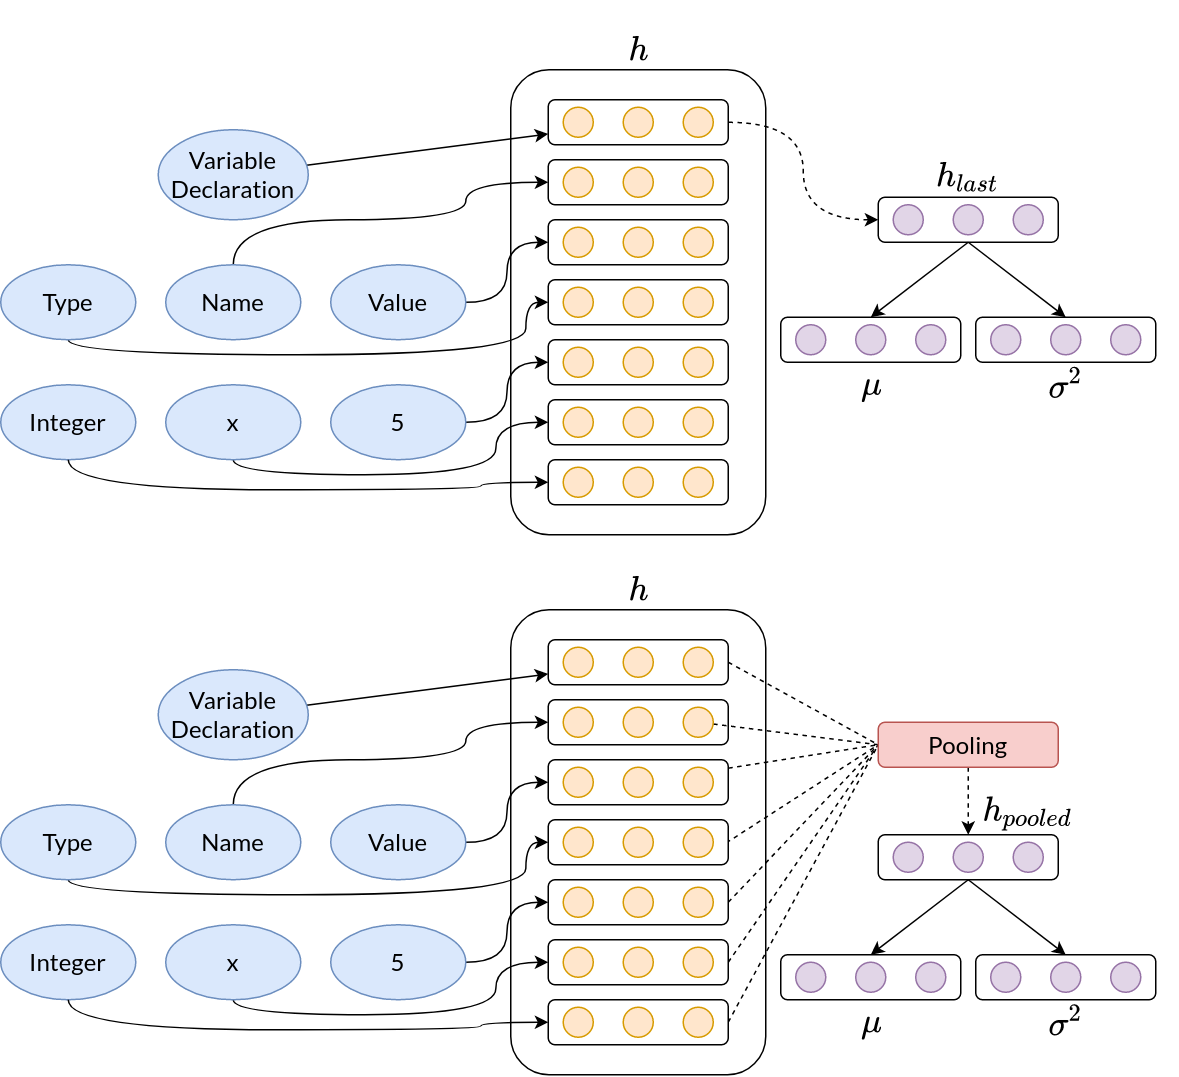
\includegraphics[width=\linewidth]{pooling.png}
    \caption[RNN pooling]{\textbf{Top}: Typical architecture of encoder model of VAE in which only the last hidden state from the RNN is used to compute the mean $u$ and variance $\sigma^2$. \textbf{Bottom}: A pooling method to aggregate the hidden states from the RNN to compute the mean $u$ and variance $\sigma^2$.}
    \label{fig:pooling}
\end{figure}




\paragraph{Neural attention} Tree-LSTM layers are followed by an attention layer. 
The node importance calculation is based on \cite{winata2018attention}, and updates the hidden states as follows:
\begin{align}
    \mathbf{h}_{at} = \mathbf{h} \odot tanh(\mathbf{W} \cdot \mathbf{h} + \mathbf{b})
\end{align}

Here, $h$ denotes the hidden states of the last Tree-LSTM layer. This additional layer allows the network to prioritize nodes that contain the most information. 


\paragraph{Pooling} 
The last step in the architecture is the pooling layer responsible for compressing the sequence of $h_{at}$ into a fixed size vector. 
We rejected a common \cite{fabius2015variational} approach of only taking the last hidden state of the RNN as the input to the decoder due to the long-term memory loss problem \cite{kao2020comparison} and use max pooling instead, see figure \ref{fig:pooling}.



\paragraph{Sampling latent code} The pooled vector is then used to compute the mean and variance of the approximate posterior to sample a latent code $z$ with the help of the reparametrization trick \cite{kingma2013auto}. The mean and variance are computed using linear layers that learn a set of weights and biases. 


\newpage
\subsection{Decoder}
The goal of the decoder network is to reconstruct a given input as accurately as possible, given the latent code produced by the encoder. 

\paragraph{Tree decoding} We use the same tree structure for decoding as we used for encoding. 
Having a reversed order of the input sequence compared to the reconstructed sequence has been shown in \cite{fabius2015variational} to improve the performance of the model. 
We employ this technique in our model, which means that since our encoder processes trees bottom-up, the decoder will produce trees top-down. 
The idea here is that the first steps of decoding the tree are more related to the latent space than the last steps.



A method called the doubly-recurrent neural network (DRNN) \cite{alvarezmelis2017tree} allows for top-down tree generation from an encoded vector representation. This method operates solely on the vector representation and does not require that either the tree structure or the nodes are given. The DRNN is based on two recurrent neural networks, breadth and depth-wise, to model ancestral and fraternal information flow. For some node $y$ with parent $pa(y)$ and previous sibling $s(y)$, the ancestral and fraternal hidden states are computed as follows:

\begin{align}
    \mathbf{h}_a^y &= rnn_a(\mathbf{h}_a^{pa(y)}, \mathbf{i}^{pa(y)}) \\ \label{eq:ancestral_update}
    \mathbf{h}_f^y &= rnn_f(\mathbf{h}_f^{s(y)}, \mathbf{i}^{s(y)}) 
\end{align}

Where $rnn_a$, $rnn_f$ are functions that apply one step of the ancestral and fraternal RNNs, respectively. Furthermore, $\mathbf{i}^{pa(y)}$, $\mathbf{i}^{s(y)}$ are the input values (label vectors) of the parent and previous sibling respectively. After the ancestral and fraternal states of $y$ have been computed with the observed labels of its parent and previous sibling, these states can be combined to form a predictive hidden state:

\begin{align}
    \mathbf{h}^y_{pred} = \tanh\left((\mathbf{W}_a \cdot \mathbf{h}_a^y + \mathbf{b}_a) + (\mathbf{W}_f \cdot \mathbf{h}_f^y + \mathbf{b}_f)\right)
\end{align}

Where the operations applied to $\mathbf{h}_a^y$, $\mathbf{h}_f^y$ are linear layers with learnable weights and biases. This combined state then contains information about the nodes' surroundings in the tree.



For each node in the tree, the model needs to decide whether it has offspring and whether it has any successor siblings. We can use the predictive hidden state of a node $\mathbf{h}^y_{pred}$, with a linear layer and a sigmoid activation to compute the probability for offspring and successor siblings as:

\begin{align}
    p_a^y &= \sigma(\mathbf{W}_{pa} \cdot \mathbf{h}_{pred}^y + \mathbf{b}_{pa}) \label{eq:prob_ancestral} \\
    p_f^y &= \sigma(\mathbf{W}_{pf} \cdot \mathbf{h}_{pred}^y + \mathbf{b}_{pf})\label{eq:prob_fraternal}
\end{align}

During training, we use the actual values for whether a node has children and successor siblings. 
During inference, we can either greedily choose any confidence level to continue creating offspring and succeeding siblings by checking whether the probability is above some threshold or sample this choice. 



Besides topological predictions, the model should also predict the label of each token. Again the predictive hidden state can be used for label prediction as follows:

\begin{align}
    \mathbf{o}^y =  softmax\left(\mathbf{W}_o \cdot \mathbf{h}_{pred}^y + \mathbf{b}_{o}\right) \label{eq:label_pred}
\end{align}


\paragraph{Tree decoding optimizations} Now that we have the basic DRNN model \cite{alvarezmelis2017tree} in place to generate a tree from scratch using a latent vector, we can optimize it for our use case. 



The first issue is the possibly infinitely large vocabulary that source code allows. Since progam behavior is invariant to identifier replacement we map each unique identifier to a reusable ID \cite{tufano2019learning} and treat the prediction of identifiers as a clustering problem between declarations and references. We use the predictive hidden states of the nodes to learn relationships between declarations and references.  



The model can keep track of a list of the declared identifiers while generating an AST. Each time a new identifier is declared, a new reusable ID is added to the list. Then for each reference, we can compute the similarity to each of the declared identifiers using some similarity function and predict the most similar identifier. We can keep track of what type of node we are currently trying to predict due to the AST structure and because we have access to the parent node label, i.e., the parent node indicates whether the child node is a declaration or reference. Let $D$ be the set of currently declared identifier nodes and $y$ be the current reference node we are trying to predict, the most similar declared identifier can be computed as follows:

\begin{align}
    \mathbf{s}^{yz} &= similarity(\mathbf{W}_c \cdot \mathbf{h}^y_{pred} + \mathbf{b}_c,  \mathbf{W}_c \cdot \mathbf{h}^z_{pred} + \mathbf{b}_c) \\
    \mathbf{r}^y &= \min_{z \in D}(\mathbf{s}^{yz})
\end{align}



We have a similar problem for literal tokens; developers can use an almost infinitely large number of unique literals in source code. However, in contrast to identifier tokens, literal tokens influence the functionality of a program. Therefore, to assure that generated programs are still compile-able, we cannot remap the literal tokens to reduce the token count. For example, we cannot map rarely used literals to special unknown tokens, as unknown tokens create compiler errors. Instead, we can employ adaptive softmax \cite{grave2017efficient} to use a vocabulary consisting of many unique literal tokens without a considerable increase in computational complexity.



We have identifiers and literals as token categories already, but we can also categorize the leftover tokens into the following categories:

\begin{itemize}
    \item \textbf{Reserved tokens:} for, if, while, ...
    \item \textbf{Types:} int, long, string, ...
    \item \textbf{Built in function names:} printf, scanf, push, ...
\end{itemize}



In total, the five categories cover all the different tokens of the programming language (at least for C++). The reason for splitting up the leftover tokens into more categories is to predict these categories separately based on their parent node. For example, this ensures that we do not input a type-token in the tree, where there should be a reserved token. The categorization improves the compilation rate of the generated programs by allowing the model only to predict tokens of the correct token category. The tree-structured representation during decoding allows us to use this optimization technique. For the reserved tokens, type, and built-in function names, equation \ref{eq:label_pred} is used for label prediction, as there is only a limited number of unique tokens in these categories. 



To allow for the categorized label predictions, we need to add one more element to the DRNN model. 
An essential aspect of the tree structure is that identifiers, built-in function names, and literals occur in the leaves of the trees. 
Hence if a node has offspring, the category of the current node must be a reserved token. 
However, if a node has no offspring, it can be either of the categories, and we need to somehow decide which category to predict a label for. Note that a reserved token can also be on a leaf node on the tree. For example, consider an empty return statement. For that reason, similar to the topology predictions, we have the model predict whether a node is of the reserved token category or not. This prediction  is computed in the same way as the topology predictions using the predictive hidden state of the node as follows: 

\begin{align}
    p_r^y &= \sigma(\mathbf{W}_{pr} \cdot \mathbf{h}_{pred}^y + \mathbf{b}_{pr}) \label{eq:res_pred}
\end{align}



\paragraph{Add gate} The DRNN model has a large flaw, where it is not able to differentiate between paths with the same prefix. For example, consider the situation depicted in figure \ref{fig:treeAddGate}, where we have two function declarations named `add' and `main'. Due to the information flow downwards, both name nodes have the same hidden state and the model is not able to distinguish the leaf nodes and will therefore predict the same label for both. This issue is depicted in the left image of figure \ref{fig:treeAddGate}. To solve this issue, we would like to incorporate the fraternal states in the downwards flow for the model to learn to differentiate the paths downwards. Hence we would like to revise eq. \ref{eq:ancestral_update}, where we take inspiration from the LSTM model and apply the idea of the add gate to our ancestral update formula as follows:

\begin{align}
    &\mathbf{m}_f^y = \sigma(\mathbf{W}_m \cdot \mathbf{h}_f^y + \mathbf{b}_m)\\
    &\mathbf{a}_f^y = tanh(\mathbf{W}_a \cdot \mathbf{h}_f^y + \mathbf{b}_a)\\
    &\mathbf{h}_a^y = \mathbf{h}_a^y + (\mathbf{a}_f * \mathbf{m}_f)
\end{align}

This update to the fraternal state is applied after predicting the label for node $y$, which is depicted in the right image of figure \ref{fig:treeAddGate}. Here, $a_f^y$ is the value of the transformation on the previous sibling state that should be added to the parent state, where the $tanh$ transforms it between -1 and +1 to mitigate exploding gradients. Furthermore, $m_f^y$ decides which elements should be added using a sigmoid function that outputs values between 0 and 1. By multiplying $a_f^y$ with $m_f^y$, the model can learn to decide what and how much to add from the previous sibling state to each parent state's element to help predict the next steps of the tree.


\begin{figure}[ht!]
    \centering
    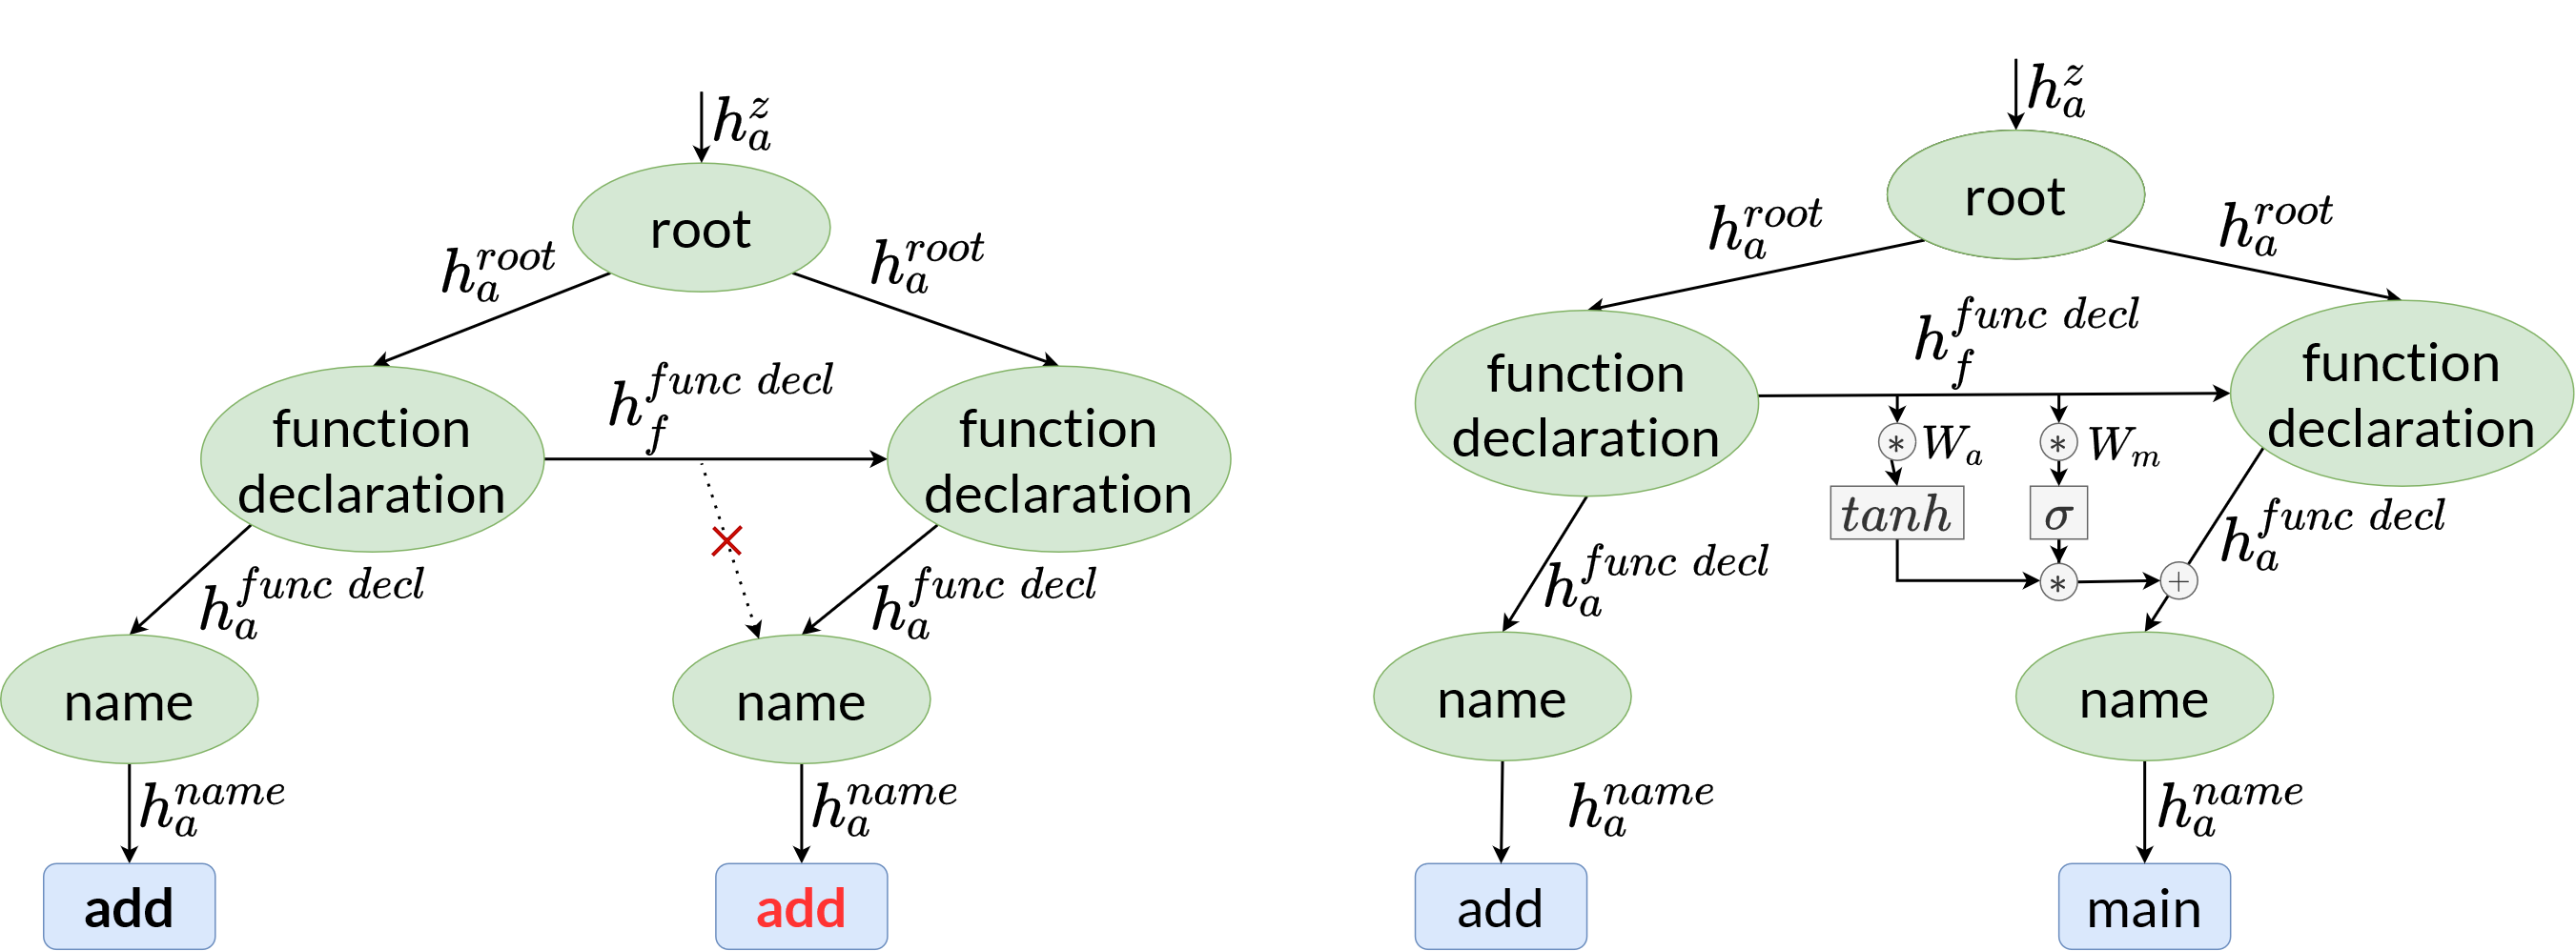
\includegraphics[width=\linewidth]{TreeAddGate.png}
    \caption{DRNN expanded with an add gate to allow for information flow from previous siblings downwards}
    \label{fig:treeAddGate}
\end{figure}

% TODO: say that the model allows for batching
% This is actually an advantage we have
%\subsection{Batching}
%We employ batching in the encoder and decoder to allow for efficient computation on GPUs. In the encoder, the computation of a node in the tree is dependent on all of its children. Therefore, the tree is processed bottom-up, and the trees can be processed in layers. For the decoder process, each node has two dependencies: the parent node and the previous sibling. Here, we process the tree top-down and from left to right at the same time. Note that each first child\footnote{With the first child, we refer to the left-most child} does not have a previous sibling. Therefore, each time a node is processed, its first child node can be computed in the next step. Moreover, because sibling nodes have the same parent, the direct successor sibling may also be computed in the next step. Hence, after processing a node, assuming the node has any offspring and successor siblings, the first child and successor sibling can be computed in the next time step.

% 

% For identifier tokens, the decoder model deviates slightly from this batching process. Because we treat the prediction of the identifier tokens as a clustering problem, we need the predictive hidden states of all the already declared identifiers when predicting a reference. A reference to an identifier may be processed before the declaration of a variable in the current setup. However, for predicting the correct label of a reference, we need to process its declaration first. Therefore, we process the identifier nodes separately, only after all other nodes have been processed. The order in which the identifier nodes are processed is from left to right within a tree, node by node. We ensure that declarations are always processed before their references by processing the identifier nodes from left to right. We parallelize this operation again across multiple trees. An example of the process is depicted in figure \ref{:treeBatchingIdentifiers}.
\newpage
\subsection{Optimization}

\paragraph{Mitigating KL vanishing}
KL vanishing is a common issue when dealing with VAEs with a decoder parameterized by an auto-regressive model.
We mitigate it vanishing using cyclical KL cost annealing \cite{fu2019cyclical}. Furthermore, we apply pooling to the hidden states of the RNN network in the encoder. Long \textit{et al.} \cite{long2019preventing} show this pooling method can effectively prevent the posterior collapse issue. 

\paragraph{Loss function}
Predicting whether a node has offspring and successor siblings are binary choices, so we can use binary cross-entropy to compute the loss for predicting the topology of the AST. 
Let $a^y$, $f^y$ represent the actual values of having offspring and successor siblings for node $y$, the topological losses for this node are then computed as follows:

\begin{align}
    \mathcal{L}_{a}(y) = - a^y \cdot \log(p^y_a) + (1 - a^y) \cdot \log(1 - p^y_a) \\
    \mathcal{L}_{f}(y) = - f^y \cdot \log(p^y_f) + (1 - f^y) \cdot \log(1 - p^y_f)
\end{align}

\noindent where $\mathcal{L}_{a}$, $\mathcal{L}_{f}$ denote the ancestral and fraternal loss respectively. Because the reserved token category prediction (eq. \ref{eq:res_pred}) is so similar to the topological predictions, the loss for that component can be defined similarly:

\begin{align}
    \mathcal{L}_{r}(y) = - r^y \cdot \log(p^y_r) + (1 - r^y) \cdot \log(1 - p^y_r)
\end{align}

\noindent where we define $r^y$ to represent the actual value of node $y$ being in the reserved token category. 



Label prediction is a classification problem for all label categories, except the identifiers.
Hence, we can compute the cross entropy loss (or negative log likelihood):

\begin{align}
    \mathcal{L}_{l}(y) = - \log(\mathbf{o}^y[l^y])
\end{align}

\noindent where we assume that $l^y$ is the index of the true label, and hence $\mathbf{o}^y[l^y]$ retrieves the softmax value at the index of the correct class. 

Lastly, since predicting the labels of identifier (reference) tokens is treated as a clustering problem, we can use triplet loss \cite{chechik2010large}. 
To compute the loss of a reference node $y$, we select the true declaration node $z$ and sample a negative declaration node $x$; the loss is then defined as follows:

\begin{align}
    \mathcal{L}_i(y)=\max(\mathbf{s}^{yx} - \mathbf{s}^{yz},0)
\end{align}

\noindent We can then combine all of the separate components to form a single reconstruction loss function for a node:

\begin{small}
\begin{align}
   \mathcal{L}_{rec}(y) = 
\begin{cases}
    \mathcal{L}_{a}(y) + \mathcal{L}_{f}(y) + \mathcal{L}_{r}(y),& \text{if } y \text{ is a declaration} \\
    \mathcal{L}_{a}(y) + \mathcal{L}_{f}(y) + \mathcal{L}_{r}(y) + \mathcal{L}_{i}(y),& \text{if } y \text{ is a reference} \\
    \mathcal{L}_{a}(y) + \mathcal{L}_{f}(y) + \mathcal{L}_{r}(y) + \mathcal{L}_{l}(y),& \text{otherwise}
\end{cases}
\end{align}
\end{small}

Because the loss is decoupled, this allows us to weigh the objectives differently to emphasize, for example, topology or label prediction accuracy. We leave experimenting with different weights for objectives as future work. 

The total loss function, combining the KL divergence, KL weight $w$ and reconstruction loss becomes:

\begin{align}
    \mathcal{L}(N) = \mathcal{L}_{tot\_rec}(N) = \sum_{y \in N}\mathcal{L}_{rec}(y) - w \cdot D_{KL}\left(Q(z|N)||P(N)\right)
\end{align}

During training, we perform teacher forcing, technique that is commonly used with sequence generation.

\begin{figure*}[ht!]
    \centering
    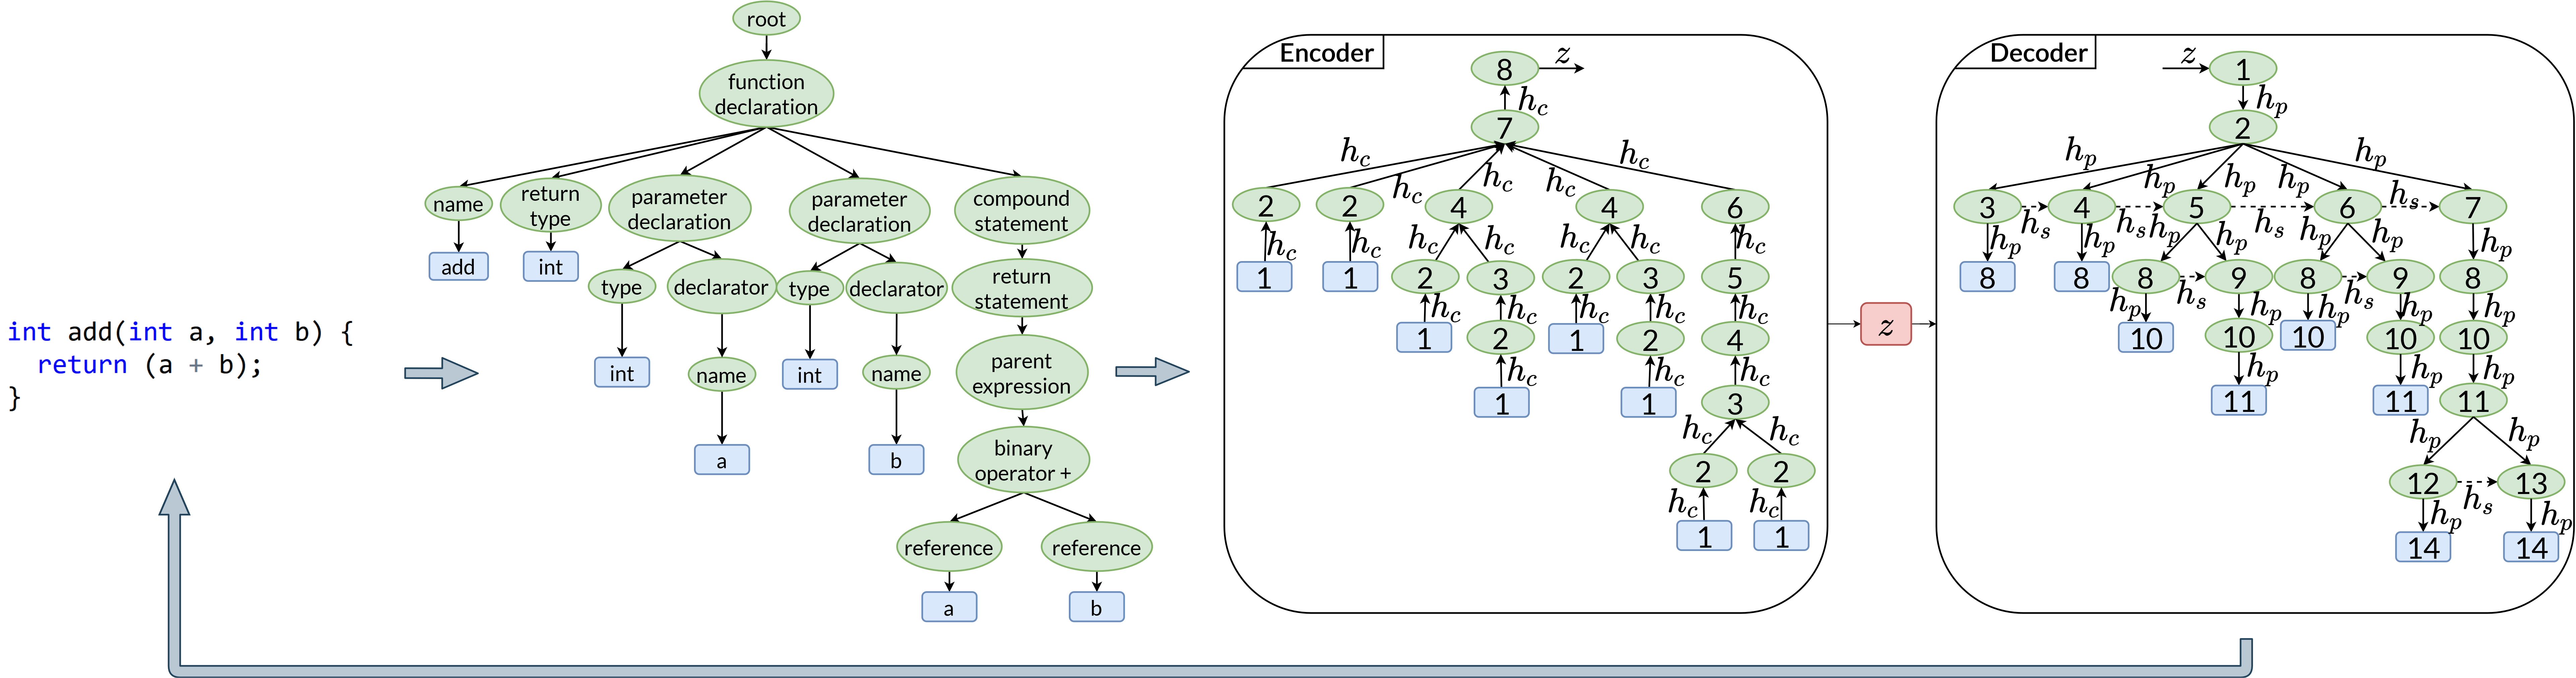
\includegraphics[width=\linewidth]{tree2treeLSTM2.png}
    \caption[Tree2Tree model high-level overview]{Tree to tree autoencoder overview. \textbf{First Fig.}: The piece of code considered. \textbf{Second Fig.}: The piece of code parsed to an AST tree format. \textbf{Third Fig.}: The order in which the encoder module encodes the tree structure bottom-up. Here, $h_c$ indicates the hidden state that travels from a child to a parent. \textbf{Fourth Fig.}: The order in which the decoder module decodes the tree structure top-down. Here, $h_p$ indicates the hidden state that travels from a parent to a child, and $h_s$ indicates the hidden state that travels from a node to its successor sibling.}
    \label{fig:tree2treeVAE}
\end{figure*}

\newpage
\section{Evaluation}
\label{evaluation}

\paragraph{Dataset}
We train and evaluate our model on a dataset of programs from code competition websites. Programs from these platforms exhibit a few qualities that are suitable for program synthesis. The programs are tested and known to be syntactically correct and compile-able, and they are standalone code fragments and do not depend on any code that is not built into the programming language. The dataset consists of almost two million C++ programs across 148 competitions divided over 904 problems. 

The programs in the data set are generally structured to contain a main function, standard input and output stream elements, computation and memory optimizations, and possibly some other elements such as helper functions/classes. Due to this general structure, the programs tend to overlap in their content, in contrast to, for example, natural language sentences. 

\paragraph{Baseline}
Our method is compared to a baseline inspired by autoencoders used for text generation in natural language. We can also evaluate how well these models generalize to source code synthesis by taking inspiration from natural language models. The model architecture is inspired from \cite{bowman2015generating}. In this architecture, both the encoder and decoder networks contain single-layer recurrent neural networks. A Gaussian prior is used for the regularization of the latent space. The model operates on the original sequences of source code and decodes the latent vector back to the source code without an intermediate structured representation. Therefore we refer to the baseline model as the Sequence-to-Sequence (Seq2Seq) model, and the architecture is depicted in figure \ref{fig:seq2seq}.

\begin{figure*}[ht!]
    \centering
    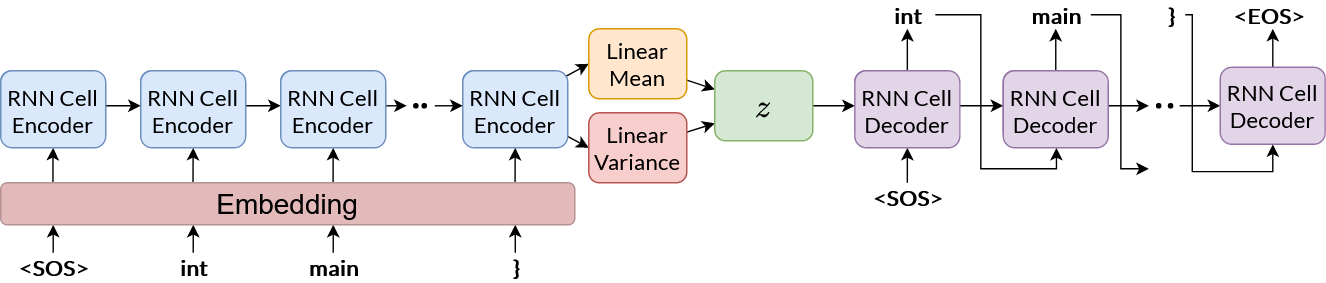
\includegraphics[width=0.8\linewidth]{seq2seq.png}
    \caption{The architecture of the Seq2Seq model}
    \label{fig:seq2seq}
\end{figure*}

Similar to our proposed autoencoder model, we employ methods to mitigate KL-vanishing. Again, we use cyclic KL annealing \cite{fu2019cyclical}, and we combine this with a technique called word dropout \cite{bowman2015generating} to weaken the decoder.

We use three-layered LSTMs in the encoder and decoder with a recurrent dropout rate of 20\% to reduce over-fitting. The embedding layer is initialized with Glove wiki gigaword 50 \cite{pennington2014glove} embedding. We train the model using the Adam optimizer \cite{kingma2014adam} with a learning rate of $1e-3$ and 10 epochs with early stopping and a patience of 3. We train and run the experiments on GPUs with a batch size set to 32.

\paragraph{Reconstruction results}\label{sec:recon-results}
First of all, we look at how accurately the autoencoders can reconstruct programs. We use a separate test split containing around 60.000 samples of our data set to evaluate this and use these samples as input for the autoencoders. 



We compute BLEU scores \cite{papineni2002bleu} for both models on the original representation of the source code to obtain comparable results, i.e., we do not use the tree representation. The Tree2Tree model thus has an extra step to use the data parser to transform the tree representation back to source code. This extra step is disadvantageous for the Tree2Tree model as it may introduce some errors due to imperfections in the parsing process. The BLEU scores are then computed on each token in a program: keywords, identifiers, operators, and special symbols such as semicolons or braces. We report on the cumulative BLEU-1 through BLEU-4 scores to indicate the overlap between original and reconstructed programs. Furthermore, we present the percentage of reconstructed programs that compile to indicate how well the models have learned the programming language's syntax. We experiment with different combinations of latent sizes $l$ and hidden RNN dimensions $h$:  ($l$:10,  $h$:50), ($l$:50, $h$:100), ($l$:100, $h$:200), ($l$:150, $h$:300), ($l$:300, $h$:500), ($l$:500, $h$:800), ($l$:800, $h$:1200).



We use greedy decoding in reconstruction experiments (table \ref{tab:rec_results}) to maximize accuracy. In contrast, sampling is used in generation tasks where diversity of candidates can be helpful.

\begin{table}[ht!]
\centering
% A table with adjusted row and column spacings
% \setlength sets the horizontal (column) spacing
% \arraystretch sets the vertical (row) spacing
\begingroup
\setlength{\tabcolsep}{3pt} % Default value: 6pt
\renewcommand{\arraystretch}{1.4} % Default value: 1
\begin{tabular}{cccccccc}
 & \textbf{Latent} & \textbf{BLEU-1} & \textbf{BLEU-2} & \textbf{BLEU-3} & \textbf{BLEU-4} & \textbf{Compiles}\\ \hline
\multirow{7}{*}{Seq}    &   10   &  0.037   &    0.024     &     0.017     &    0.013       &    0.000\%   \\
                            &   50   &      0.085    &      0.061         &         0.047      &    0.037       &       42.467\%      \\
                            &   100   &  0.295   &      0.225     &     0.176      &    0.141       &   65.808\%               \\
                            &   150   &     0.278  & 0.211          & 0.165          & 0.131          &  66.971\%              \\
                            &   300   & 0.346                     &  0.262                        &     0.203                     &     0.161                     & 60.651\% \\   
                            &   500   &  0.421                   &      0.332                    &         0.263                 &      0.211                    &  90.329\% \\
                            &   800   &  0.429                   &      0.329                    &         0.253                 &      0.195                    &  \textbf{91.784\%} \\\hline
\multirow{7}{*}{Tree}  &   10   &  0.445  &    0.339     &     0.260     &     0.202      &   28.375\%    \\
                        &   50   &     0.417    &      0.317    &       0.242    & 0.189  &  23.256\% \\
                            &   100   &     0.423      &      0.323     &     0.251      &  0.200 &      30.429\%     \\
                            &   150   & \textbf{0.486} &     \textbf{0.382}    &  \textbf{0.302}     &      \textbf{0.243}    &   35.419\%           \\
                            &   300   &   0.457                 &     0.342                &      0.260                &     0.202                   & 35.054\% \\   
                            &   500   &     0.398                &      0.301             & 0.230      &             0.178             &            36.022\%      \\
                             &   800   &     0.258                &      0.182             & 0.131      &             0.096             &     2.358\%      \\
\end{tabular}
\endgroup
\caption{Reconstruction results.}
\label{tab:rec_results}
\end{table}

The results listed in table \ref{tab:rec_results} show the superiority of the Tree2Tree model in terms of reconstruction capability (BLEU scores), especially for smaller latent sizes. The reconstruction scores of the Tree2Tree model of latent size 150 outperform all the Seq2Seq models up to latent size 800. In contrast, the Seq2Seq models show to perform much better at constructing compile-able programs, which improves with the model's size, to nearly 100\%. This is a surprising result, which is investigated in more detail in section \ref{evaluation}.

 


An interesting result is that the performance of the models does not necessarily increase with the size of the model. Especially for the Tree2Tree models, we see that after latent size 150, the models' performance decreases. In general, one would expect that the model would perform better with an increase in latent size, allowing more information flow between the encoder and decoder. We hypothesize that, because not only the latent size increases but also the number of hidden units in the auto-regressive models, the models experience KL vanishing. Due to the increasing hidden units, the auto-regressive models become stronger and may depend more on their predictions, ignoring information from the latent vector. In turn, the reconstruction performance vastly decreases. Confirmation of this hypothesis is left as a venue for future work.



Next, we would like to experiment on how different input sizes affect the performance of both models. Due to the tree-structured representation used by the Tree2Tree model, the size of the sequences that the RNNs process scale proportionally to the width and depth of the tree. The Seq2Seq model, on the other hand, processes sequences left to right, hence the number of computations of the RNNs scale directly with the sequence length. 



To evaluate the performance on different sized inputs, we split the test data set into three subsets. A small, medium and large subset with the following properties:

\begin{itemize}
    \item \textbf{small subset}: maximum of 250 tokens
    \item \textbf{medium subset}: between 251 and 500 tokens
    \item \textbf{large subset}: between 501 and 750 tokens
\end{itemize}

 

We compute the BLEU scores and compilation percentage again using greedy decoding on the smaller subsets for the best performing Seq2Seq and Tree2Tree models, based on the results of table \ref{tab:rec_results}. Here, performance is based on the combination of BLEU-4 and compilation percentage. For Seq2Seq, this is the model with latent size 500. Similarly, for Tree2Tree, this is the model with latent size 150. The results are depicted in table \ref{tab:rec_results_inp_sizes}.



%150 latent t2t lr 0.001 large test set (> 500, <= 750): bleu1 0.317, bleu2 0.236, bleu3 0.177, bleu4 0.134, compiles 5.001

%150 latent t2t lr 0.001 medium test set (> 250, <= 500): bleu1 0.468, bleu2 0.364, bleu3 0.284, bleu4 0.225, compiles 21.241


\begin{table}[ht!]
\centering
% A table with adjusted row and column spacings
% \setlength sets the horizontal (column) spacing
% \arraystretch sets the vertical (row) spacing
\begingroup
\setlength{\tabcolsep}{3pt} % Default value: 6pt
\renewcommand{\arraystretch}{1.4} % Default value: 1
\begin{tabular}{clccccc}
 & \textbf{Input} & \textbf{BLEU-1} & \textbf{BLEU-2} & \textbf{BLEU-3} & \textbf{BLEU-4} & \textbf{Compiles}\\ \hline
\multirow{3}{*}{Seq}    &   small   &   0.513  &    0.403    &      0.321    &  0.258      &  95.334\%     \\
                            &   medium   &  0.306      &    0.244        &      0.192     & 0.153      & 86.812\% \\
                            &   large   &    0.196   &      0.157   &   0.123       &   0.096       &  87.971\% \\ \hline
\multirow{3}{*}{Tree}  &   small   &   0.633  &    0.516     &     0.424     &     0.355      &  59.022\%                \\
                            &   medium   &   0.478  &   0.371        &          0.289 &     0.229   & 21.241\%            \\
                            &   large   &  0.324 &      0.242  & 0.181    &    0.138     &    5.001\%         \\ 
\end{tabular}
\endgroup
\caption{Reconstruction results of the best models on different input sizes.}
\label{tab:rec_results_inp_sizes}
\end{table}



From table \ref{tab:rec_results_inp_sizes} we can observe that both models follow the same logical trend: the larger the input size, the lower BLEU-scores and compilation percentages. For the Tree2Tree model, the BLEU scores for the medium subset seem to be similar to the BLEU scores on the entire test set, whereas, for the Seq2Seq model, the BLEU scores are much lower on the medium subset. The models seem to be fairly close in terms of performance degradation from small to large program sizes. For example, we can measure performance degradation for the large versus small subset by dividing the BLEU-4 scores on the large set by the BLEU-4 score on the small set. For the Seq2Seq model, we get a score of $0.372$, and for the Tree2Tree model, we get $0.389$. Similarly, we get $0.593$ and $0.645$ for the Seq2Seq and Tree2Tree model for the medium versus small subset. While the performance degrades less with increasing input sizes for the Tree2Tree model, this difference is insignificant. 



An issue with the aforementioned computation of performance degradation is that it does not correct for elements in programs that are almost always present. For example, each program contains a main function, with standard input and output streams. The models may simply always predict these standard elements of a program and then use the information of the encoder to complete the details of the program. However, this causes the BLEU score to consist of two parts: the score for the prediction of the elements that are always present and the score of what it has learned to predict together with the encoder. The latter is more interesting and shows how much information can be saved in the latent vector. 



Therefore, we apply a correction on the BLEU scores to focus on the prediction based on the information in the latent vector. We compute corrected scores by feeding the decoder with random latent vectors and computing BLEU scores on the subsets of the test data set. Then, we subtract these correction scores from the computed BLEU scores in table \ref{tab:rec_results_inp_sizes}, and take 0 if the result of the subtraction is negative. The corrected BLEU scores including the correction scores are presented in table \ref{tab:corrected_rec_results_inp_sizes}.

\begin{table}[ht!]
\centering
% A table with adjusted row and column spacings
% \setlength sets the horizontal (column) spacing
% \arraystretch sets the vertical (row) spacing
\begingroup
\setlength{\tabcolsep}{3pt} % Default value: 6pt
\renewcommand{\arraystretch}{1.4} % Default value: 1
\resizebox{\linewidth}{!}{%

\begin{tabular}{clccccc}
\textbf{Model}   & \textbf{Input size} & \textbf{BLEU-1} & \textbf{BLEU-2} & \textbf{BLEU-3} & \textbf{BLEU-4} \\ \hline
\multirow{3}{*}{Seq2Seq}    &   small   &   0.072 (0.441)  &    0.077 (0.326)    &  0.075    (0.246)    &  0.070 (0.188)     \\
                            &   medium   & 0.006 (0.300)      &  0.018  (0.226)        &    0.021  (0.171)     & 0.023 (0.130)    \\
                            &   large   &   0.000 (0.213)   &  0.000    (0.166)   & 0.000  (0.128)       &  0.000 (0.099)   \\ \hline
\multirow{3}{*}{Tree2Tree}  &   small   &  0.200 (0.433)  &  0.220  (0.296)     &  0.223   (0.201)     &    0.218 (0.137)        \\
                            &   medium   &  0.148 (0.330)  &  0.147 (0.224)        & 0.146 (0.150) &    0.128 (0.101)        \\
                            &   large   &  0.102 (0.222) &    0.090  (0.152)  &  0.079 (0.102)     &  0.070  (0.068)      &   \\
\end{tabular}%
}
\endgroup
\caption{Corrected BLEU scores of reconstructed results of the best models on different input sizes. (correction scores in parenthesis)}
\label{tab:corrected_rec_results_inp_sizes}
\end{table}



Table \ref{tab:corrected_rec_results_inp_sizes} indicates a large difference in performance degradation between the Seq2Seq model and the Tree2Tree model. A noticeable result is that the corrected BLEU scores for large programs predicted by the Seq2Seq model are 0. Hence, the Seq2Seq model extracts no information from the latent vector at all for large programs. Similarly, for medium-sized programs, little information is transferred between the encoder and decoder. We can again compute the performance degradation scores for the Seq2Seq model, which are $0.280$ and $0.00$ for the medium versus small and large versus small subsets, respectively, on the corrected BLEU-4.



In contrast, the performance degradation is much smaller for the Tree2Tree model:  $0.587$ and $0.321$ for the medium versus small and large versus small subsets, respectively, on the corrected BLEU-4. Hence, the structural nature of the Tree2Tree model scales better to large input sequences than the Seq2Seq model in terms of reconstruction scores, even with a much smaller latent size. 



An interesting observation is that the latent vector conveys relatively little information in terms of BLEU scores. The correction scores make up a large part of the total BLEU scores as presented in table \ref{tab:rec_results_inp_sizes}. Hence, the BLEU scores are largely determined by the models' general knowledge of how C++ programs are built up and not the specific content.

\paragraph{Generative results}
\label{results:gen}
To see how well autoencoders can generate reasonable samples from any point in latent space that conform to the C++ syntax, we sample 1000 random latent vectors from the prior distribution $\mathcal{N}(0, I)$ and input these vectors to the decoder networks. Then, we compute the percentage of generated programs that compiles and is thus also syntactically correct.



We employ two decoding strategies to test the generative capabilities of the models: greedy decoding and sampling. The sampling strategy we apply is a combination of top-$k$, nucleus, and temperature sampling \cite{holtzman2019curious}. We first use temperature sampling to scale the logits to control the shape of the probability distribution. Then, we filter the on the top-$k$ samples, after which we filter tokens on their cumulative probability using nucleus sampling (top-$p$). Lastly, we sample a token from the resulting distribution. The selected sampling hyper-parameters for this experiment are: $k=40$, $p=0.9$, $temperature=0.7$. The results of the experiment are displayed in table \ref{tab:gen_results}.

\begin{table}[ht!]
\centering
% A table with adjusted row and column spacings
% \setlength sets the horizontal (column) spacing
% \arraystretch sets the vertical (row) spacing
\begingroup
\setlength{\tabcolsep}{3pt} % Default value: 6pt
\renewcommand{\arraystretch}{1.4} % Default value: 1
\begin{tabular}{cccc}
\textbf{Model}   & \textbf{Latent size} & \textbf{Greedy search} & \textbf{Sampling} \\ \hline
\multirow{5}{*}{Seq2Seq}    &   10   &  0.0\%   & 0.9\%  \\
                            &   50   &   38.5\%    &  2.9\%   \\
                            &   100   &   62.1\%   &  21.3\%     \\
                            &   150   &   58.0\%  &     23.5\%        \\
                            &   300   &  60.6\%  &  36.8\%   \\   
                            &   500   &  67.5\% & 37.8\% \\
                            &   800   & 78.2\%  & 39.6\% \\\hline
\multirow{5}{*}{Tree2Tree}  &   10   &   29.6\%   & 20.2\% \\
                            &   50    & 22.6\%   &  17.7\%    \\
                            &   100    & 30.3\%  &       22.1\%      \\
                            &   150  &  26.9\%  &   18.8\%     \\
                            &   300  & 23.4\%  & 12.8\%    \\   
                            &   500 & 25.6\%  & 14.4\%\\
                            &   800   &  4.1\% & 6.7\% \\
\end{tabular}
\endgroup
\caption{Generative results compilation percentage.}
\label{tab:gen_results}
\end{table}




The results from table \ref{tab:gen_results} show similar trends as section \ref{sec:recon-results}. The general trend is: the larger the model (in terms of latent size and hidden units), the higher the compilation percentage. Moreover, greedy search during inference gives a higher compilation percentage than sampling. This outcome is not surprising, as, with greedy search, we always pick the label for which the model is most confident. On the other hand, sampling gives a more varied output and may be useful for searching similar programs in a vicinity of the latent space. The trade-off for a more diverse output is thus a lower compilation ratio. 

\newpage
\section{Conclusion}

Our results indicate that Tree Variational Autoencoders have a significant advantage over sequence-to-sequence models in low-dimensional latent spaces, achieving both a higher compilation rate and a higher reconstruction quality.
In higher-dimensional latent spaces seq2seq programs offer a higher compilation rate, but based corrected BLEU scores indicate that this benefit is often achieved by sacrificing reconstruction quality, even to the point of ignoring the input completely.

Overall, our findings support the initial hypothesis that structured autoencoder models are better suited for program synthesis than sequence-to-sequence alternatives.
We believe this result to be a significant step towards an autoencoder-based foundation model for genetic programming and genetic improvement of software.


\newpage
\chapter{Multiagent Programming with LLMs}\label{ch:seidr}
\chapter{Multiagent Programming with LLMs}
\label{ch:seidr}

\todo{Ensure standard nomenclature}

\section{Introduction}
\label{sec:seidr-intro}

Two recent innovations potentially make the latter task tractable.

One is \emph{Synthesize, Execute, Debug}~\cite{gupta2020:synthesize}, a framework that attempts to bridge the ``last mile'' gap by introducing program repair into the program synthesis algorithm. 
A programming task is specified using both a natural language description and a set of input/output (I/O) pairs that demonstrate what output is expected from the program, thereby combining text-to-code~\cite{iyer2018:mapping} and programming by example~\cite{halbert1984:programming,gulwani2016:programming} paradigms typical for competitive programming~\cite{zavershynskyi2018:naps}.
\emph{Synthesize, Execute, Debug} creates a first draft program using a generative model, compiles and executes it with given input examples.
This is followed by a program repair step to fix the identified errors.

Another relevant innovation is instruction fine-tuned large language models~\cite{zhang2024:instruction}. Instruction fine-tuned models use human feedback in their training process and are designed to explicitly or implicitly admit two inputs: a source text (or code) and a textual command instructing the model to edit the source in a particular way, e.g., ``summarize'' or ``translate to Python.''
These models have been shown to be highly successful in automatic program repair~\cite{fan2023:automated}. 
However, given the free-form nature of these instructions, how one should engineer instructions that maximize repair performance is an open question. 

These innovations have led to the proposal of a framework, \emph{Synthesize, Execute, Instruct, Debug and Rank}, or SEIDR,\footnote{~Seiðr also refers to a type of Norse magic~\cite{blain2002:nine} pertaining to predicting and controlling the future, which we deem thematically appropriate.} initially introduced in our GECCO-2023 paper~\cite{liventsev2023:fully}. 
%The current paper partly reiterates the methodology and findings of~\cite{liventsev2023:fully} and expands on them in this extended version of the original paper.
SEIDR is a multi-agent iterative framework that uses feedback from code execution and failing test cases to update the initially generated buggy code. 
Our initial explorations cover SEIDR with GPT-3 as the bug summarization model and Codex (or GPT-3 trained on code) as the program generation and debugging model.  
% We test a number of prompting strategies for LLMs to fix a working prompt.
In addition, by modifying the tree arity parameter (see Section~\ref{sec:seidr-beam-search}), we investigate the trade-off between generating and repairing only one program versus regenerating any program that does not pass all the tests, as well as intermediate configurations, where we build a tree of programs and update the best ones.

While Codex is an early code generation model, the emergence of new models that score better in programming and natural languages motivates further research into the use of SEIDR with newer models. 
To study the generalizability of the initial SEIDR results, we use two other LLMs, Llama 3\footnote{~\url{https://ai.meta.com/blog/meta-llama-3/}} and GPT-3.5,\footnote{~\url{https://openai.com/form/researcher-access-program/}} and an additional dataset, HumanEval-X, with different tree arity parameters~\cite{brown2020:language, chen2021:evaluating, zheng2023:codegeex}. 
Moreover, we build up on the initial experiments with Codex and zoom in on the area with the best-performing tree arities in a hyperparameter search for a better repair-replace trade-off resolution. 

To reflect on the parent selection strategies used in the Rank agent of SEIDR, we also explore whether the programs should be chosen based on the average performance across all tests or whether SEIDR can benefit from keeping such programs in the loop that fully cover individual tests, but do not perform well on average.
Therefore, as an alternative to the tournament selection, we test the best tree arity setups with lexicase selection-based ranking~\cite{helmuth2015:solving}.
Moreover, since language models bring in stochasticity, we run the experiments several times to measure the variability of results obtained with fixed hyperparameters and reflect on the results repeatability.

Overall, the current paper contributes to the field of Large Language Models for Software Engineering (LLM4SE) with a framework for code generation and its iterative repair. 
Compared to the earlier GECCO-2023 paper, this article refines and extends the preliminary results by providing a more in-depth explanation of SEIDR as a multi-agent framework for autonomous programming, extending the original experiments and analysis to include HumanEval-X as an additional benchmark, evaluating GPT-3.5 and Llama 3 as additional LLMs, investigating lexicase selection as an alternative to tournament selection, and conducting a repeatability analysis of the framework’s performance over multiple independent runs. Overall, this extension adds three research questions and doubles the number of configurations considered in these questions compared to our preliminary work. 

Section~\ref{sec:seidr-methodology} presents a framework that adapts \emph{Synthesize, Execute, Debug} to instruction-tuned Large Language Models in agents that can solve programming tasks in an autonomous fashion. 
We discuss related work in Section~\ref{sec:seidr-related-work}, introduce experiments to explore effective search 
% and prompting 
strategies for this framework in Section~\ref{sec:seidr-eval}. 
Finally, in Section~\ref{sec:seidr-results}, we demonstrate that our framework outperforms conventional automatic programming techniques, such as genetic programming and naive application of large language models that generate one solution per problem without updating it iteratively. 

\section{Methodology}
\label{sec:seidr-methodology}
The proposed five-agent SEIDR framework is summarized in Figure~\ref{fig:method}, which we discuss in detail in Section~\ref{sec:seidr-ingredients}.
In essence, to solve a programming task defined as a text description and a collection of I/O examples, we split I/O examples into prompt and validation sets and use the prompt set in a large language model to SYNTHESIZE a population of candidate solutions.
We EXECUTE the solutions, test them against the validation set, generate a text description of the identified problems used to INSTRUCT a large language model to produce repaired candidate solutions similar to the way a human developer DEBUGs a program.
We RANK the candidates
by correctness, measured as matching I/O pairs, discard the worst candidates, and repeat until a fully correct solution is found.

\begin{figure}[t]
    \centering
    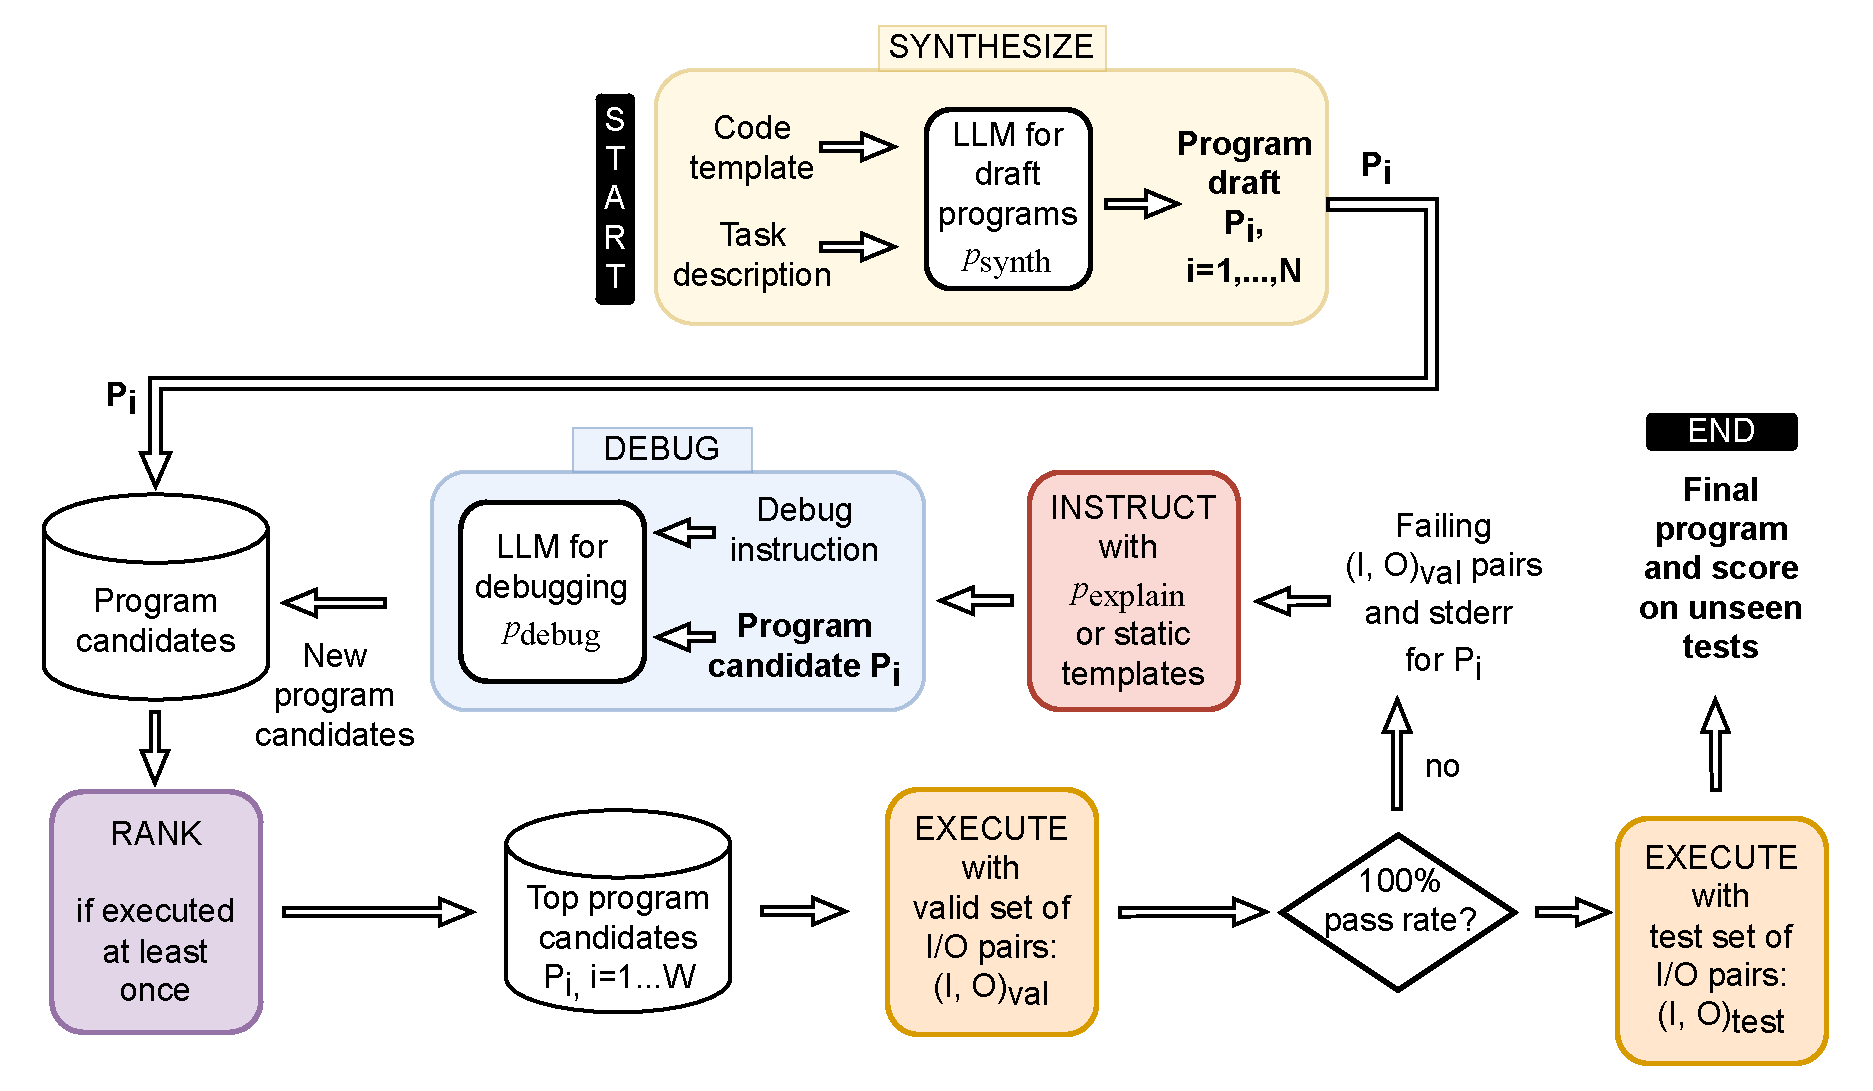
\includegraphics[width=\linewidth,trim={0mm 0mm 0mm 0mm}]{images/codex-for-psb-seidr-methodology-5.drawio.pdf}
    \caption{Overview of SEIDR, a multi-agent iterative framework that uses LLMs to implement the Synthesize, Execute, Instruct, Debug, and Rank feedback loop.}
    \label{fig:method}
\end{figure}
 

\subsection{Ingredients}
\label{sec:seidr-ingredients}

SEIDR makes use of instruction fine-tuned large language models: a \emph{synthesis} model $p_{\text{synth}}(\text{code, }$ descr), a \emph{debugging} model $ \langmodel_\text{debug} $, as well as a model $ \langmodel_\text{text} $ that can be used for writing textual instructions, which are forwarded to the code generation model $ \langmodel_\text{debug} $ for code updates. 
Therefore, the design can be described as two agents communicating with each other, whereby one generates code and another provides critical or supervising comments on what should be changed in the generated code. 

The models $ \langmodel_\text{synth} $, $ \langmodel_\text{debug} $, and $ \langmodel_\text{text} $ can be either separate or the same model.
The prerequisites are that $ \langmodel_\text{synth} $ and $ \langmodel_\text{debug} $ models are able to ``understand'' natural language (descr) and partial or full programs (code) and generate code based on them. 
The model $ \langmodel_\text{text} $ should be able to ``understand'' code and natural language and either autocomplete or generate the debugging instruction from scratch. 
Note that $ \langmodel_\text{text} $ is optional, since alternatively the debugging instructions can be generated from failing tests using static pre-defined templates.
%as described in~\cite{liventsev2023:fully}. 
In general, SEIDR requires sequence-to-sequence generative models for these agents. 
%In our experiments, we have chosen models $ \langmodel_\text{synth} $, $ \langmodel_\text{debug} $, and $ \langmodel_\text{text} $ that are based on the state-of-the-art transformer architecture~\cite{vaswani2017:attention} as a backbone and its subsequent improvements (see Section~\ref{sec:seidr-models}). 
In our experiments, we select models for $ \langmodel_\text{synth} $, $ \langmodel_\text{debug} $, and $ \langmodel_\text{text} $ based on the state-of-the-art transformer architectures~\cite{vaswani2017:attention} 
%and its subsequent improvements 
(see Section~\ref{sec:seidr-models}). 

Each LLM is a highly parameterised probability distribution over the space of (code, description)-tuples with parameters estimated on a large diverse (i.e., non-task-specific) corpus.
This stochastic nature of language models is an important prerequisite for SEIDR, since it allows us to sample batches of diverse candidate solutions from $ \langmodel_\text{synth} $, $ \langmodel_\text{debug} $, and $ \langmodel_\text{text} $. 
We denote the number of outputs generated with $\treearity_\text{draft},$ $\treearity_\text{debug},$ and $\treearity_\text{explain},$ correspondingly.
Moreover, each model generates the most probable and less probable outputs in each batch, which helps diversify problem solving attempts. 
In the following implementation-related subsections, we explain how we vary the number of candidate solutions, debug instructions, and repairs generated in a batch by each LLM in SEIDR.

While SEIDR is described here as a multi-agent system, it can equally be seen as a form of evolutionary algorithm or genetic programming, where the initialization and mutation steps of the system are performed by LLMs, $ \langmodel_\text{synth} $ and $ \langmodel_\text{debug} $, correspondingly.
Throughout this work, we use agent-oriented programming terminology~\cite{shoham1993:agentoriented} and evolutionary optimization terminology interchangeably to try to bridge the gaps between these domains.

\subsubsection{Synthesize}
\label{sec:seidr-synth}

The framework starts with the SYNTHESIZE agent, which is responsible for generating initial draft solutions.
% to programming tasks to be repaired in later stages of SEIDR.
We start with a basic template for a chosen programming language that contains a number of standard library imports, as shown in Figure~\ref{fig:template}.

\begin{figure}[t]
    \centering
    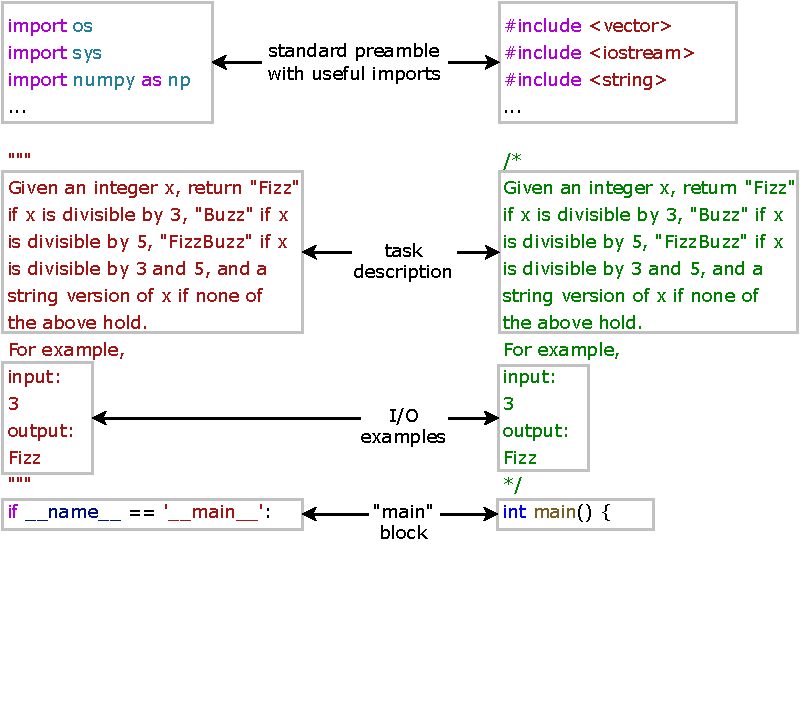
\includegraphics[width=0.8\linewidth, trim={0mm 40mm 0mm 0mm}, clip]{images/Templates-new-v2.pdf}
    \caption{Anatomy of SYNTHESIZE templates}
    \label{fig:template}
\end{figure}

We populate this template with a comment indicating a textual task description and several I/O examples from the training set.
We design the templates with prompt engineering guidelines\footnote{~\url{https://platform.openai.com/docs/guides/prompt-engineering/six-strategies-for-getting-better-results}} and prior work~\cite{debruin2021:autoencoders} in mind.
We then sample $\treearity_\text{draft}$ programs from $ \langmodel_\text{synth} $, setting \texttt{code} to the populated template and \texttt{description} to the natural language description of what the model should generate.
We use spring sampling:\footnote{~\url{https://vadim.me/publications/spring/}} a temperature-based sampling with a monotonically increasing temperature schedule where the $i$-th program is sampled with temperature $t_i \approx \frac{i-1}{\treearity_\text{draft}}$ (we use approximate equality to enable efficient implementation by means of batching).
Thus, the sampling procedure for the first programs approximates a deterministic maximum-likelihood estimation.
%Ultimately, this approach ensures that samples are diverse, but always contain the likeliest programs.
In combination with the naturalness principle of source code \cite{allamanis2018:survey,jiang2022:bugs}, this approach ensures that the samples are diverse, but always contain the most likely programs for the given task.

%Consider the following search problem:

\begin{figure}
    \centering
    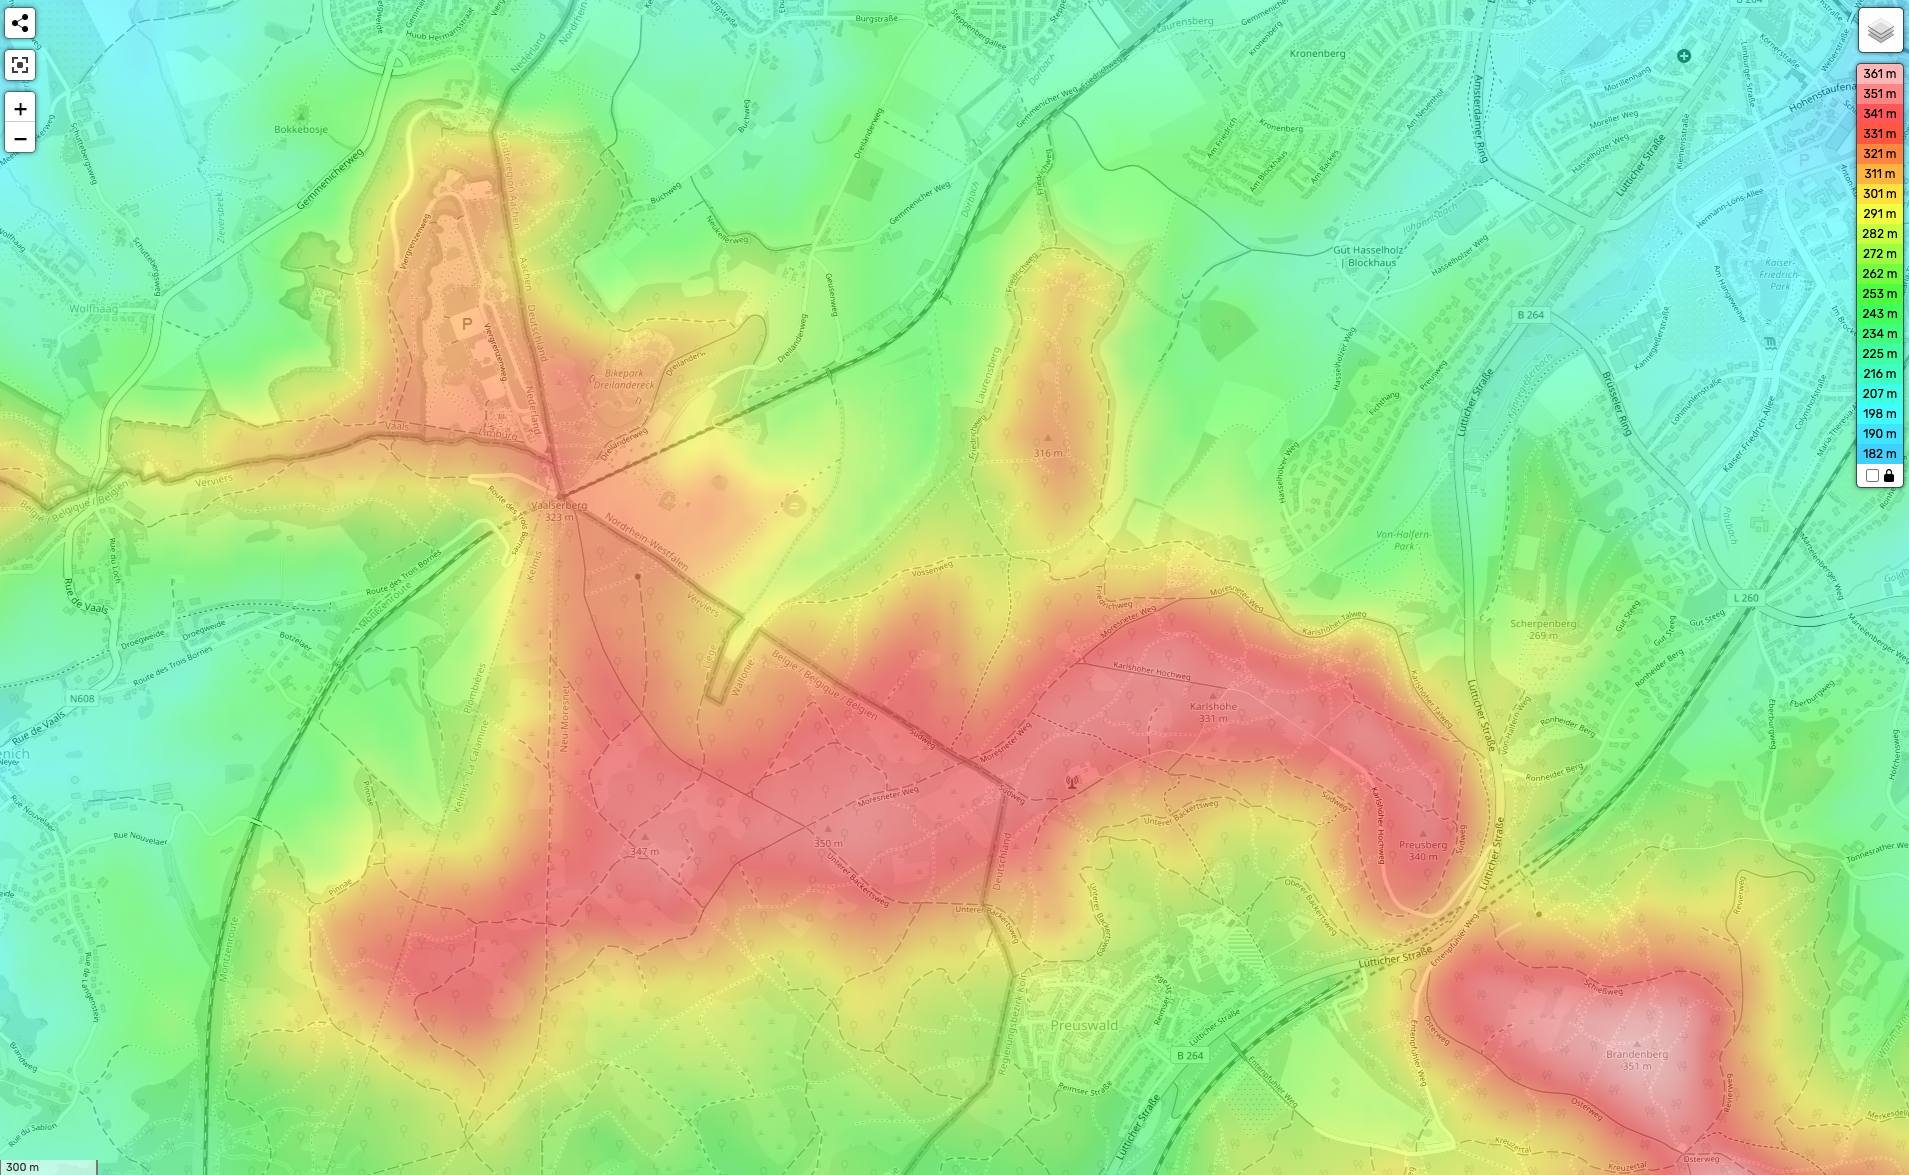
\includegraphics[width=0.8\linewidth]{images/vaalserberg_lost.png}
    \caption{Vaalserberg elevation map}
\end{figure}


The above elevation map of Vaalserberg\footnote{\url{https://en.wikipedia.org/wiki/Vaalserberg) (the hill that acts as a three-way border between Belgium, the Netherlands and Germany}} contains a telecommunications tower. Can you find it? Hint: in a hilly terrain, telecommunication towers work better when they are higher up.

If you are anything like me, you would start by looking at the highest points on the map.
If the tower is not there, you would move your gaze (more or less randomly) around the highest parts of the map.
If it's still not found, you would gradually include lower and lower parts of the map into the search space covered by the random walk of your gaze.
At some point, if you still don't see the communications tower, your gaze will be dashing all over the map, including the lowest points.

Let us now formalize this algorithm mathematically.

The height above sea level of a point on this map is a heuristic function that represents the probability $p(x)$ of a telecommunications tower being located at point $x$.
We can search the area by sampling points $x \sim p(x)$ and checking whether a tower is present at $x$, i.e. whether $t(x)=1$.
We can control how much attention we give the high elevation/high likelihood points versus low elevation/low likelihood points with a technique known as **temperature sampling**: define temperature $t$ and sample from a modified distribution

\begin{equation}
p_t(x) = \frac{p(x)^{\frac{1}{t}}}{\sum_{x'} p(x')^{\frac{1}{t}}}
\end{equation}

When $t=0$ we always sample the global maximum: the single likeliest point on the map. 
When $t=1$ $p_t(x)=p(x)$.
The higher the temperature $t$ the more attention is given to the less likely points in the distribution.

Hence, the technique of looking at the likeliest points first, then gradually including less and less likely ones, corresponds to the following algorithm. At iteration $i$ of our algorithm we sample from the distribution $p_t(x)$ where temperature is given by

\begin{equation}
t = i \Delta t
\end{equation}

where $\Delta t$ is a hyperparameter that controls the heat input into the system, directly proportional to how impatient the searcher is. So,

\begin{equation}
x \sim p_t(x) = \frac{p(x)^{\frac{1}{i \Delta t}}}{\sum_{x'} p(x')^{\frac{1}{i \Delta t}}}
\end{equation}

We call this technique **spring sampling**, as it involves gradually, but continuously adding heat to the system until life wakes up therein.

Spring sampling can be used in any **informed search problem** (aka heuristic search problem): find an $x$ such that $t(x)=1$ given a heuristic function $p(x)$ estimating the probability that $t(x)=1$. 
Informed search often comes up in conjunction with machine learning: many machine learning models are probability distributions $p(x)$ that estimate how likely some statement is to be true.
For example, a model for ImageNet classification \cite{dengImagenetLargescaleHierarchical2009} us a distribution $p(i,c)$ indicating how likely it is that image $i$ belongs to class $c$.
Likewise, language models are probability distributions $p(w_1,\dots,w_n)$ indicating how likely it is that sentence $w_1,\dots,w_n$ is appears in the training corpus and/or satisfies the human feedback annotator.
A particularly topical (but far from the only) application of spring sampling is thus using a large language model agent to achieve a certain testable goal: sample from the LLM with increasing temperature until the output passes the test.
We use this technique in our program synthesis framework to sample programs that pass a given test suite.
It improves search speed by making sure the likeliest programs are always tested first, but if they don't pass the test, higher temperatures help collect a diverse sample of programs, thus increasing the probability that one of them is correct.

Meanwhile, did you find the tower? Here it is:

\begin{figure}
    \centering
    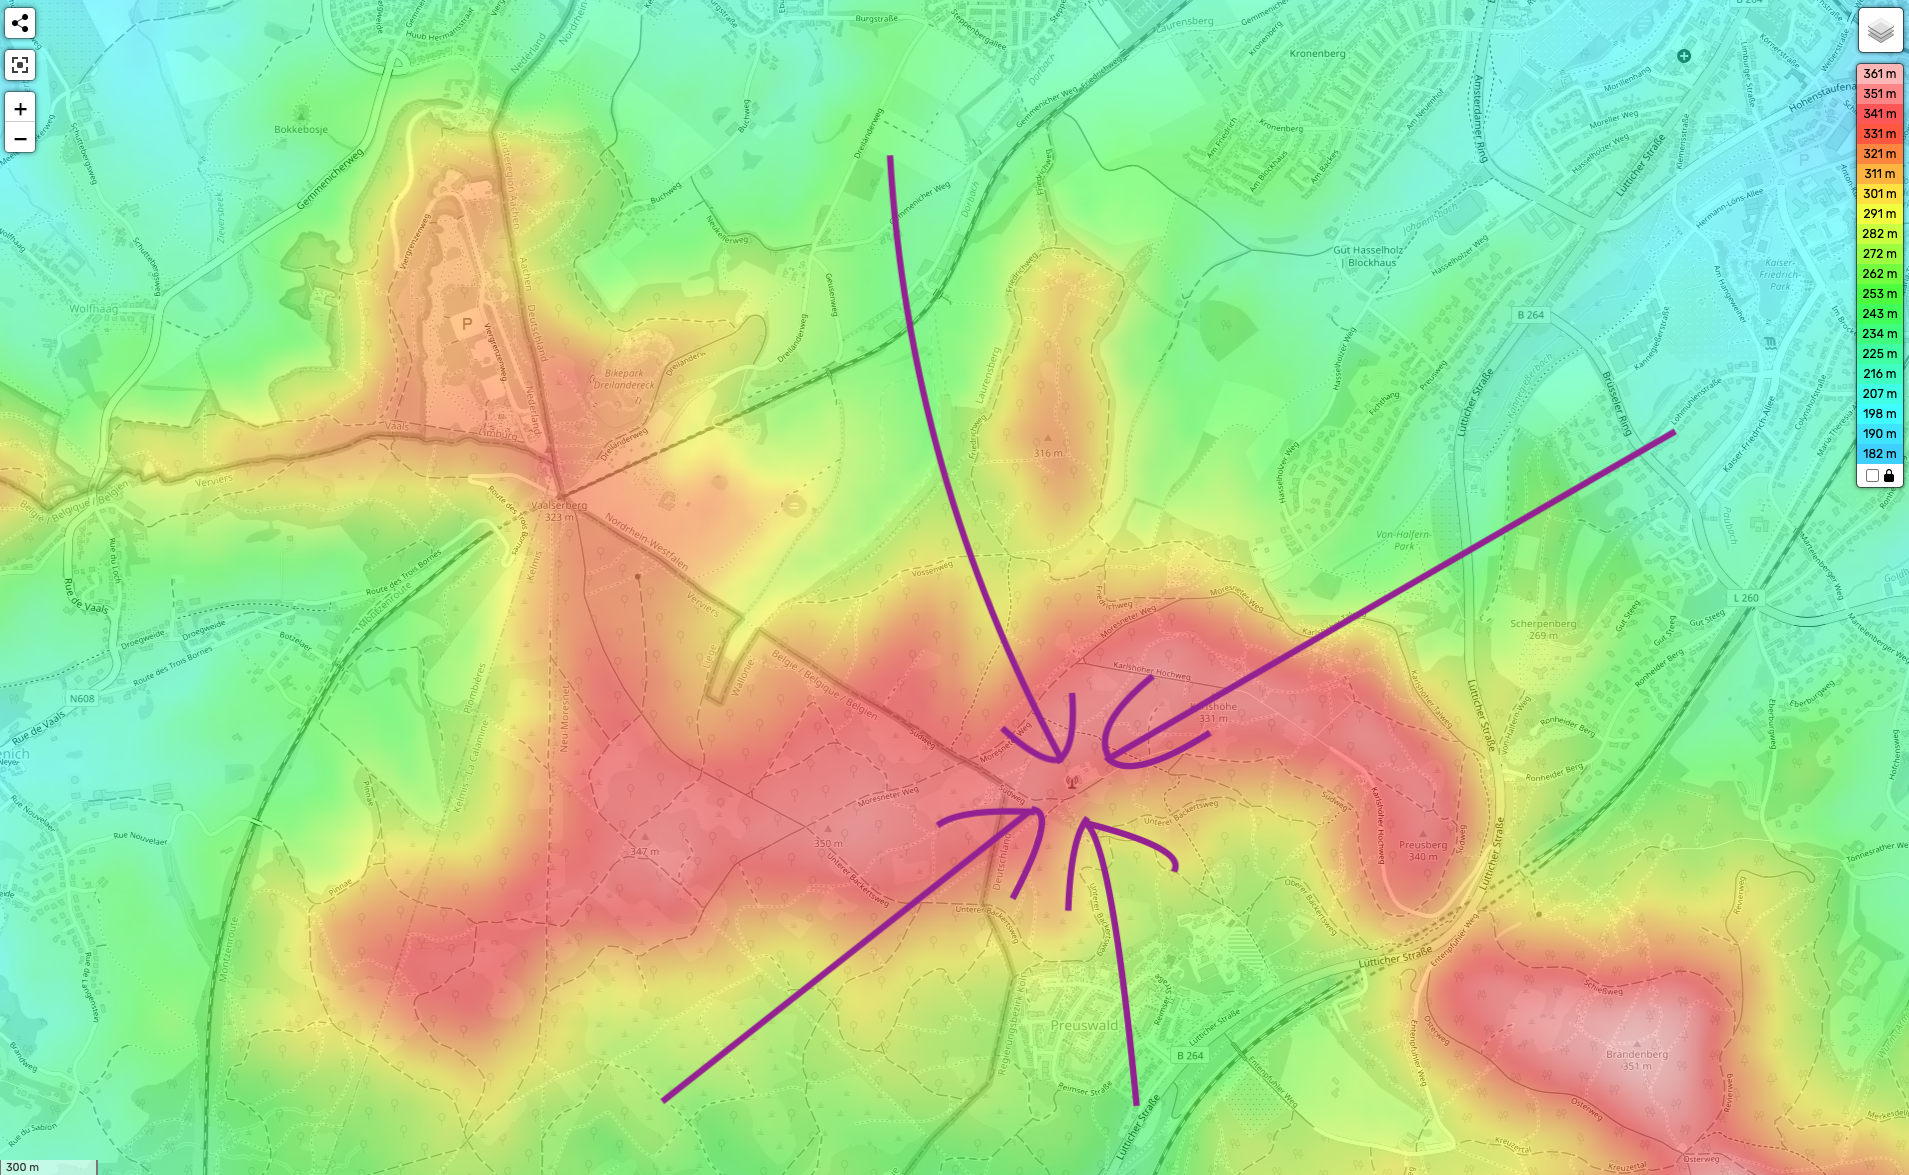
\includegraphics[width=0.8\linewidth]{images/vaalserberg_found.png}
    \caption{Vaalserberg elevation map, tower highlighted}
\end{figure}


\subsubsection{Execute}
\label{sec:seidr-execute}

\todo{Holy war on the letter n}

The EXECUTE agent compiles the programs (if necessary) and launches them using the standard tools for the programming language.
The program is run once for every I/O pair in the validation set. 
Its \texttt{stdin} stream receives all input lines in a given input pair, and its \texttt{stdout} and \texttt{stderr} streams are captured and saved.
We then measure the \emph{score} of the program defined as the accuracy over the output lines, with \expoutputvec{} being the expected output, and $n=\max\{|\expoutputvec{}|, |\text{stdout}|\}$:
\[    
\text{score}(\expoutputvec{}, \text{stdout}) = \frac{\sum^{n}_i{\mathbb{I}[\text{stdout}_i = O_i]}}{n} 
\]
unless \texttt{stderr} is non-empty during compilation or execution, which is considered to indicate failure and is assigned a score of 0.

\subsubsection{Instruct}
\label{sec:seidr-instruct}

The goal of the INSTRUCT agent is to provide instructions that summarize bugs in a candidate program and suggest a solution for $ \langmodel_\text{debug} $. 
The resulting instructions with the bug summary should indicate what requirement is violated and instruct the LLM to edit the candidate program accordingly. 
The input to INSTRUCT consists of failing I/O pairs from the validation set and \texttt{stderr} output of the candidate execution. 
In order to represent this heterogeneous input as text that can be further processed by an LLM, we use template engines that replace placeholders in files or strings with input values and return a formatted string. 
In recent chat- and instruction-based LLMs, the terms \emph{template engine} and \emph{prompt template} are used interchangeably.

We consider two different designs of the INSTRUCT agent: INSTRUCT$^{\text{static}}$ and INSTRUCT$^{\text{LLM}}$ shown in Figure~\ref{fig:method-instruct}. 
In both cases, if \texttt{stderr} is not empty, i.e., execution exits with code 0 before getting any output to compare it with the expected output, the \texttt{stderr}-based template engine generates the instruction to fix the error. 
However, the designs differ in the way they transform failing I/O pairs to generate instructions in case \texttt{stderr} is empty.

\begin{figure}[t]
    \centering
    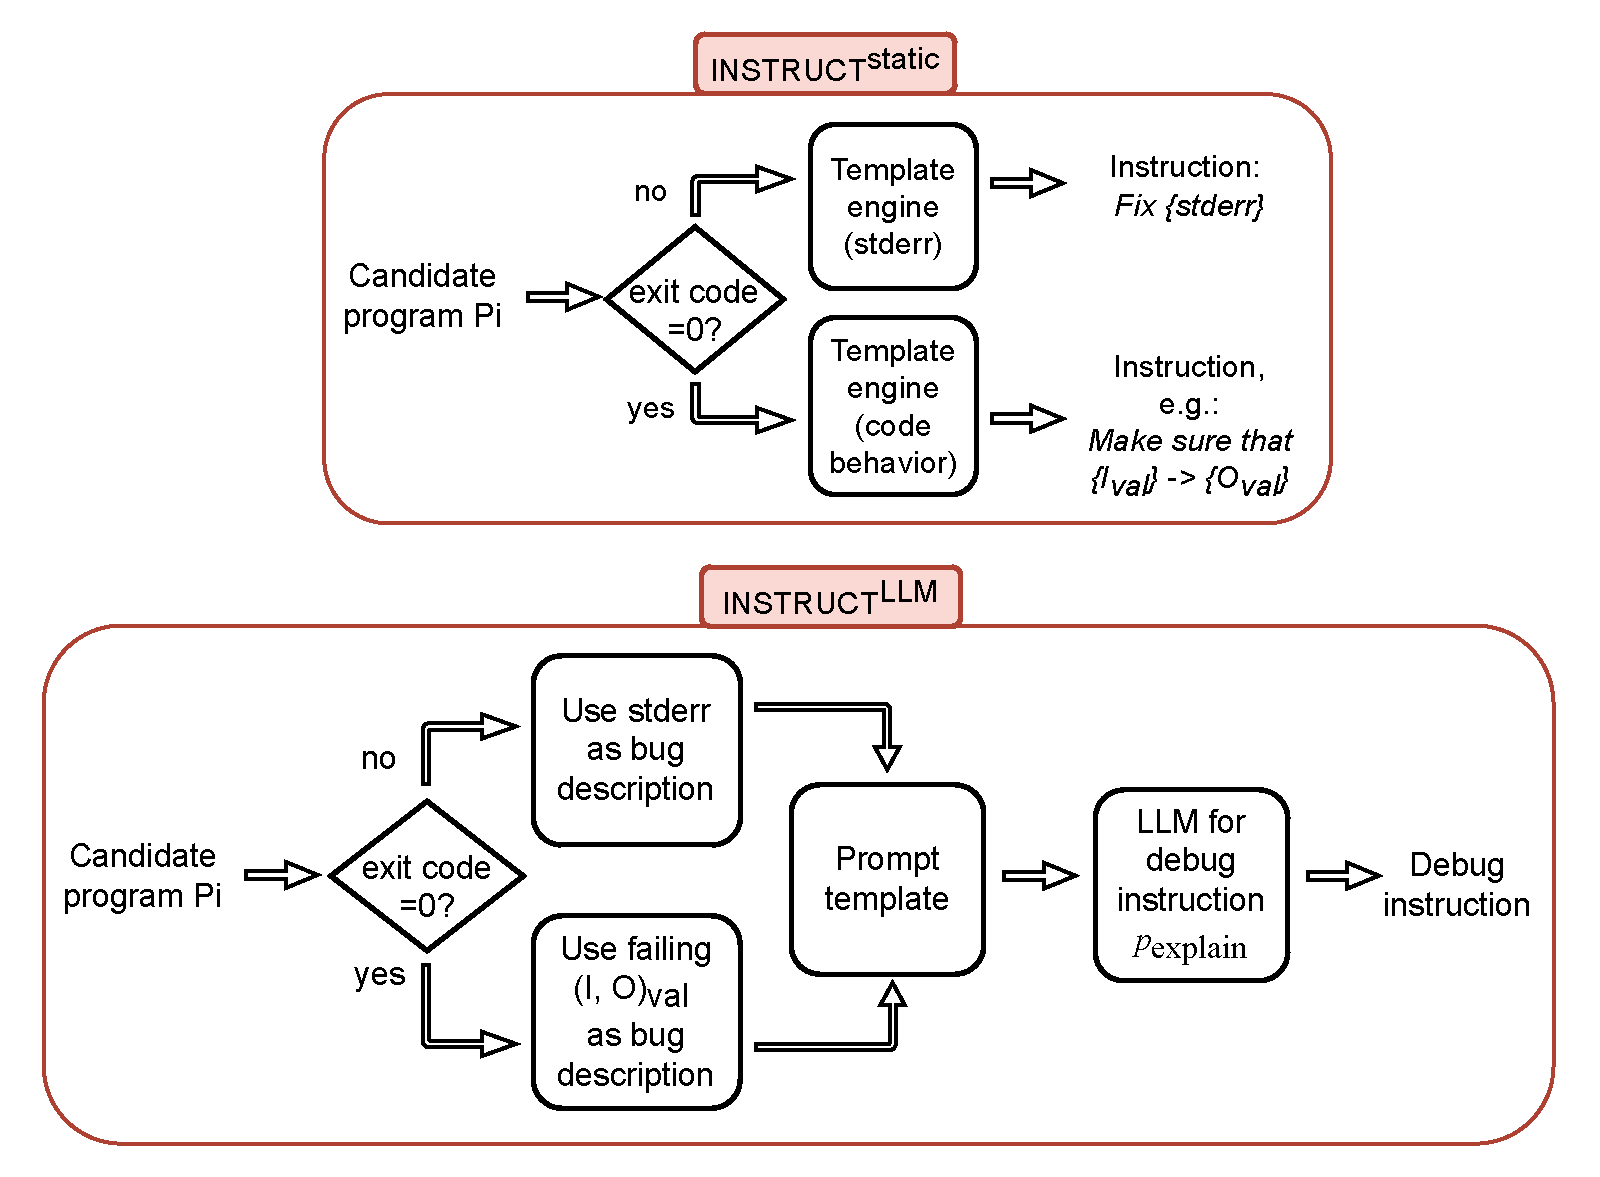
\includegraphics[width=0.85\linewidth,trim={0mm 0mm 0mm 0mm}]{images/codex-for-psb-seidr-instruct-2.drawio.pdf}
    \caption{Overview of the two designs for the INSTRUCT agent.}
    \label{fig:method-instruct}
\end{figure}

INSTRUCT$^{\text{static}}$ uses a fixed template and substitutes placeholders for input and output with the corresponding strings of the first failing test case in its template engine.
For example, we show the resulting instruction for an exemplar template in Figure~\ref{fig:method-instruct}.
In contrast, INSTRUCT$^{\text{LLM}}$ uses the failing I/O pair in the LLM for text completion, thereby prompting the text LLM to produce the bug explanation and a summary for debugging. 
In addition to providing a failing test case or \texttt{stderr}, one may choose to give the model $ \langmodel_\text{text} $ more context, such as the problem name, task description, and the code generated so far. 
Each call to $ \langmodel_\text{text} $ can result in $\treearity_\text{explain}\ge1$ instructions, a batch output of an LLM.
The prompt templates used for the experiments are detailed in Section~\ref{sec:seidr-prompts}.

% An exemplar output of the code behavior template engine in Figure~\ref{fig:method-instruct} describes that the code returns output O instead of expected output O$_{\text{val}}$ for the failing test case with input string I$_{\text{val}}.$
% The LLM is then prompted to auto-complete this description of program behavior with the bug summary. 
% The bug summary is passed further to the next template engine that uses it as debugging instruction, such as ``\emph{Fix \{bug summary\}}''.

\subsubsection{Debug}

The main component of SEIDR that addresses the ``near-miss syndrome'' is the DEBUG agent.  
This agent iterates over all programs in the population to repair candidate programs and pass more tests. 
It uses the instructions written by INSTRUCT to sample from the $ \langmodel_\text{debug} $ model $\treearity_\text{debug}$ times
to repair each candidate and create a new population of \treearity{} candidates.
For $ \langmodel_\text{debug} $, the parameter \texttt{code} is set to the current version of the candidate solution and \texttt{descr} to the output of INSTRUCT and any additional context chosen for a specific implementation.
The current generation of candidates is then replaced by \treearity{} outputs of DEBUG.

\subsubsection{Rank}

The RANK agent implements what is known in genetic programming as \emph{parent selection}~\cite{koza1994:genetic}: it selects the best $\beamwidth{}$ programs to be further improved by the DEBUG agent.
We consider two different parent selection algorithms: tournament selection and lexicase selection. 
See Section~\ref{sec:seidr-lexicase-results} for their empirical comparison.

\emph{Tournament selection} variant used in this work sorts the programs according to their average test score and selects top $\beamwidth{}$ candidates. 
% Such ranking approach is a \emph{quality-based} selection method.
The programs are selected based on the intuition that repair of the best so far (yet imperfect) programs begets good programs. 
The simple ranking is also referred to as \emph{tournament selection}, where the best-performing candidates are chosen to participate in the next round.  
In the classical tournament selection, the first step is to draw $n$ random candidates from the population. 
In our implementation, the first step is to generate exactly $n$ candidates that are needed for the next round. 
This approach prioritizes candidates that perform the best on average over all tests.
% At the same time, tournament selection does not favor candidates that pass fully one or several tests but may not have a high average test pass rate score. 

\emph{Lexicase selection}~\cite{helmuth2015:solving} is a ranking approach that maximizes the diversity of selected candidates in addition to their metric-based score.
Lexicase selection ensures diversity by keeping the program candidates that perform the best on unique tests as opposed to the program candidates that perform best on average over all tests.
The algorithm is as follows:
\begin{enumerate}

\setlength{\parskip}{0pt}
\setlength\itemsep{0pt}

    \item randomly shuffle the set of tests;
    \item select a program with the best score on test 1;
    \item if several programs are tied, resolve the tie by selecting the best program on test 2;
    \item repeat for tests $3,4,\dots,$ until only one program is left;
    \item mark this program as ``selected'';
    \item if less than $\beamwidth$ programs are selected, go back to step 1.
\end{enumerate}
This ensures that even if the average quality of the selected candidates is lower, the batch of $\beamwidth{}$ programs collectively contains a higher number of required ``skills'', as measured by tests.



\subsection{Meaning of Hyperparameters}
\label{sec:seidr-beam-search}

\begin{figure}[t]
    \centering
    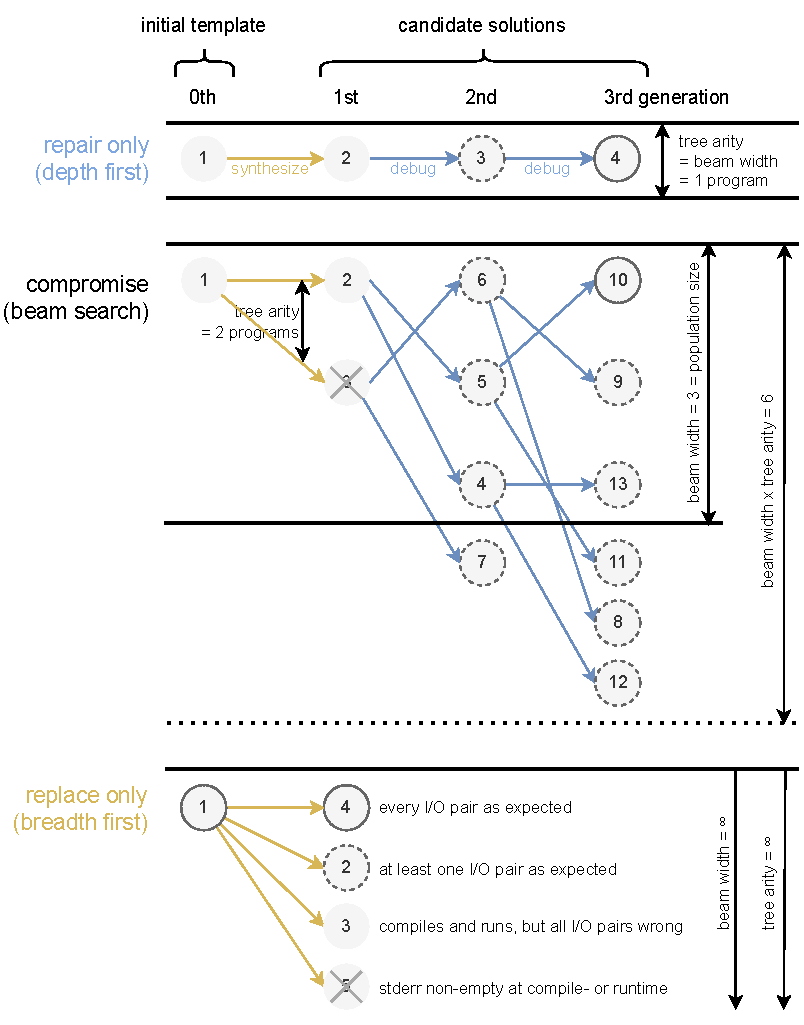
\includegraphics[width=0.7\linewidth, trim={0mm 4mm 0mm 0mm}]{images/beamsearch.pdf}
    \caption{Repair-replace trade-off as a tree search problem.}
    \label{fig:beam-search}
\end{figure}

After evaluating a given candidate solution in EXECUTE, SEIDR supports two approaches to address the candidate's flaws:
\begin{itemize}
\setlength{\parskip}{0pt}
\setlength\itemsep{0pt}
  \item \emph{Replace} the candidate with another sample from the current population.
  \item Use INSTRUCT and DEBUG to repair the candidate.
\end{itemize}
We refer to this problem as the \emph{repair-replace trade-off}, by analogy with production economics~\cite{jack2000:optimal}. 

How does the choice of hyperparameters $\treearity{},$ the total number of candidate programs in each generation, and $\beamwidth{},$ the number of selected repairs to be preserved in a generation, influence the flow of SEIDR?
$\treearity$ and $\beamwidth{}$ act as upper bounds on the \emph{replace} option by limiting the size of the population.
In the edge cases, $\treearity{} = \beamwidth{} = 1$ corresponds to a repair-only process, while $\treearity{} = \beamwidth{} = \infty$ corresponds to replace-only, as illustrated in Figure~\ref{fig:beam-search}. 
Here, the repair-only scenario can also be seen as an LLM-guided random walk~\cite{xia2020:random} and replace-only as random sampling from the LLM.
Strategies with tree arities between $1$ and $\infty$ are similar to population-based evolutionary algorithms.
Note that $\treearity{}$ is defined by $\treearity_\text{draft}$ for the initial draft solutions in the first generation and $\treearity_\text{explain} \cdot \treearity_\text{debug}$ for later generations. 

Observe that a mutation-only genetic algorithm with tournament selection with fixed population size $\beamwidth{},$ such as SEIDR, is equivalent to \emph{local beam search} with beam width $\beamwidth{}$ on an $\treearity{}$-ary tree ~\cite[Section 4.1.4]{russell2010:artificial}. This corresponds to a known property of local beam search: it degenerates into a depth-first search at $\beamwidth{} = 1$, whereas setting $\beamwidth{} = \infty$ yields a breadth-first search.

% Hence, we refer to $\treearity{}$ as \emph{tree arity} and $\beamwidth{}$ as \emph{beam width}.

\section{Related Work}
\label{sec:seidr-related-work}

% Changes: explicit author surnames, order and some phrasing

Until recently, the tasks of neural program synthesis~\cite{gulwani2017:program} and program repair~\cite{legoues2019:automated, petke2018:genetic, legoues2012:systematic,zhang2024systematic} have been considered separately.
However, results from genetic programming~\cite{sobaniaRecentDevelopmentsProgram2021} suggest that evolution is a crucial step in synthesis.
A number of important studies bridging this gap in the application of large language models have been carried out concurrently with this work, discussed below.

The use of large language models for a program repair step within a program synthesis pipeline has been studied by \cite{joshi2022:repair:arxiv} and \cite{gupta2020:synthesize}, 
while the specific case of instruction-driven LLMs has been explored by \cite{fan2023:automated}, where the initial synthesis is done by the Codex model~\cite{chen2021:evaluating} and for program repair both Codex and state-of-the-art specialized repair tools such as TBar and Recoder~\cite{just2014:defects4j} are considered and compared. 
\cite{zhang2023:selfedit} do the same, but fine-tune PyCodeGPT-110M~\cite{zan2022:cert} to use it as a repair model. 
The resulting framework is a two-step process (1 draft step and 1 debug step), while iterative evolution and search are not explored. 

Evolution through Large Models (ELM)~\cite{lehman2022:evolution} proposes to use a language model in place of a mutation operator within a traditional genetic programming framework~\cite{koza1994:genetic}. They use a type of instruction fine-tuned model trained on git commit messages known as a diff model.\footnote{~\url{https://carper.ai/diff-models-a-new-way-to-edit-code/}}
%~\cite{DiffModelsNew2023}. 
However, the model is directed neither to solve the programming problem at hand nor to fix bugs.
Instead, it is provided with generic instructions such as ``Change function f.'' 
This approach is meant for the cases where creative freedom~\cite{stanley2015:why} is encouraged rather than satisfying concrete requirements.
\cite{liu2023algorithm} demonstrate the advantages of applying ELM to modular components of a solution, rather than the entire solution to the given problem.

Some related work is explicitly guided by the metaphor of conversation between agents. 
\cite{zhang2023steam} implements a repair-only program synthesis loop as a conversation between an analyst agent, a coder, and a tester, while \cite{dong2024:selfcollaboration} does the same for tester, developer, and reviewer. 
The coder and the developer are roughly equivalent to SYNTHESIZE, the tester to EXECUTE, and the reviewer to INSTRUCT, while the analyst is an agent that prepares a generation prompt for the coder. 
Both testers are language models that predict the output of a program without actual compilation, execution, or testing, which makes \cite{dong2024:selfcollaboration} and \cite{zhang2023steam} specific cases of chain-of-thought prompting~\cite{yu2023:better} for program synthesis.

Several studies explore an iterative approach to program synthesis in a manner similar to SEIDR~\cite{xia2023:conversational,chen2023:teaching,shinn2023:reflexion}. 
However, they do not explore the repair-replace trade-off and exclusively implement the repair-only approach that is prone to local minima.
SelfEvolve~\cite{jiang2023:selfevolve} is a repair-only version of a framework similar to SEIDR.
SeflEvolve demonstrates the benefits of LLMs evolving not just the source code but an additional natural language text file that acts as the system's knowledge base and is included in the model prompt when generating code. 
Finally, Self-Taught Optimizer (STOP)~\cite{zelikman2023:selftaught} takes the concept of self-improvement to the meta level and uses a large language model to edit the evolutionary algorithm itself (i.e., blocks or contents of Figure~\ref{fig:method}). 
Their reflections on the safety implications of such automated algorithm changes are of particular interest when considering this trajectory~\cite[Section 8]{zelikman2023:selftaught}. These concerns do not hold in the context of SEIDR because the algorithm is fixed.
In other words, SEIDR does not self-evolve but creates solutions that it improves, and the solutions that are synthesized are closely constrained by the validation set used by the EXECUTE agent.
% that will prevent FizzBuzz from scheming a planetary takeover.

These efforts to combine large language models and evolutionary techniques fall within the broader context of the quest for effective inductive bias in genetic programming~\cite{whighamSearchBiasLanguage1996}: a crucial property for any learning algorithm~\cite{haussler1988:quantifying}. 
\cite{reuterGraphNetworksInductive2023} suggest using graph neural networks for this purpose, while grammatical evolution methods, such as WHGE~\cite{bartoliWeightedHierarchicalGrammatical2020} and $\pi$-GE~\cite{oneill2004:pgrammatical} use the known grammar of the programming language.
Large language models are a novel and promising~\cite{custodeComparingLargeLanguage2024} alternative to grammatical evolution that incorporates semantics and idiom~\cite{allamanisMiningIdiomsSource2014,orlovFindingIdiomsSource2020} of a programming language in addition to its grammar. 

\section{Experimental Design}
\label{sec:seidr-eval}

To explore the capabilities of SEIDR and its generalizability, we test the framework on two benchmarks (PSB2 and
HumanEval-X), a total of two different ranking strategies (tournament selection and lexicase selection),
three models in the coding part of SEIDR (Codex, GPT-3.5, and Llama 3), two programming languages (Python and C++), and various branching factors.
We use three models over the two parts of our experiments: one model in the initial exploration (also reported by~\cite{liventsev2023:fully}) and two models in the generalizability part.
The problems in the benchmarks originate from coding competitions and human-written programming assignments. 

During our empirical evaluation of SEIDR, we address the following research questions:
\head{\rqtreearity{}. Repair-replace trade-off exploration} 
What is the impact of using different tree search strategies
in the autonomous programming setting? 
We experiment with six different tree arities but fix the tournament selection in the ranking part and one prompt. 
Here, we study the impact of tree arity on the number of resolved problems as well as the speed of obtaining solutions.   
% \head{RQ2. Prompt engineering} What is the effect of using LLM-produced bug summaries compared to static instructions on the repair of automatically synthesized code? We test six static debug instructions that describe bug behavior based on violated requirements and five dynamic debug prompt templates auto-completed with LLMs. 
\head{\rqllama{}. Generalizability of the approach to different LLMs and an additional dataset} 
How does the choice of an LLM affect the performance of SEIDR? 
We vary the tree arity and experiment with two additional LLMs and one additional dataset.
By default, we use tournament selection as the ranking strategy. 
\head{\rqmultirun{}. Repeatability of SEIDR in multiple runs with the same hyperparameters} 
How does the non-deterministic nature of LLMs affect SEIDR performance when the method is restarted several times with the same hyperparameters?
We study how SEIDR results vary in different restarts of the same experiments with unchanged hyperparameters as a result of the LLM non-determinism. 
The motivation for \rqmultirun{} is that LLMs exhibit stochastic behavior: the same prompt can yield different responses. 
Essentially, LLMs generate answers token-by-token and predict the next tokens based on the probability distribution over a vocabulary of tokens, which is sensitive to the precision of floating-point operations. 
If two tokens are predicted to be the next ones, with a very similar probability, it is likely that either of them will be chosen at each individual run. 
Further tokens are generated auto-regressively and depend on the previous tokens, so once one token diverges, the whole sequence is likely to diverge, too. 
\head{\rqlexicase{}. Effect of changing the parent selection strategy in the RANK agent}
How does the lexicase selection-based ranking strategy impact performance in comparison to tournament selection in the RANK agent? 
We use the best-performing tree arities from \rqmultirun{} to run the experiments with lexicase selection as the ranking strategy instead of tournament selection, to explore whether a different parent selection algorithm can further improve the results.


\subsection{Data}
\label{sec:seidr-data}

Our experiments use the Program Synthesis Benchmark~2 (PSB2)~\cite{helmuth2022:applying} and HumanEval-X~\cite{zheng2023:codegeex} in C++ and Python. 
The key criteria for this choice are the availability of task descriptions in English and unit tests in Python and C++ or language-agnostic unit tests as well as the wide acceptance of these benchmarks in the areas of generative LLMs (HumanEval) and genetic programming (PSB2). 

\subsubsection{PSB2}
The first dataset is a benchmark suite of 25 problems for program synthesis that resemble small real-world tasks. PSB2 was developed as a more realistic and challenging version of PSB1~\cite{helmuth2015:general}, the latter consisting of textbook problems and is widely used in genetic programming~\cite{sobania2022:choose}. 
The problems require different data structures and control flows to be used for effective solutions and are taken from sources, such as competitive programming platforms and educational courses. 
The problems have descriptions in English, as well as 1 million~(M) tests for training and 1M testing-stage tests, including edge or corner cases that test the resulting program on complicated inputs. 
The tests are provided as I/O pairs and are distributed together with the problem descriptions as a PyPI package.\footnote{~\url{https://pypi.org/project/psb2/}} 

In PSB1, the training set consists of the edge test cases and is augmented by random test cases if the number of edge tests is not enough. The test set is formed by random test cases. 
This terminology is preserved in PSB2.
We use the PSB2 training set for ranking and selection of programs (validation) within an experiment and the test set for reporting the result thereof (testing).
Thus, we will refer to the PSB2 training set as the \emph{validation set}, to be more consistent with how it is used in SEIDR.

\subsubsection{HumanEval-X}
The second dataset that we use is a development from the original set of human-written programming tasks in HumanEval~\cite{chen2021:evaluating}, which is a standard code generation benchmark for LLMs.
HumanEval consists of 164 problems with a docstring representing problem description, a function signature, a correct solution, and unit tests in Python. 
HumanEval-X is the result of translating correct HumanEval programs and unit tests into five programming languages~\cite{zheng2023:codegeex}. 
We use HumanEval-Python for experiments in Python to ensure a comparison with other models in the setup without SEIDR. 
In addition, we test SEIDR on the HumanEval-C++ part of HumanEval-X. %here and in an earlier SEIDR study~\cite{liventsev2023:fully}. 

The test functions of HumanEval-X contain all tests in one function. We split the aggregated test functions into separate tests so that the RANK agent can evaluate the \text{score}. 
On average, the number of tests in HumanEval-Python is 7.25 and 6.95 in HumanEval-C++, which is appointed to a repeated additional test present in some HumanEval-Python examples of the following type: \texttt{assert True, "This prints if this assert fails 1 (good for debugging!)"}.
This test type is not present in HumanEval-C++.

To reiterate, we keep the original HumanEval-Python setup for direct comparison with the models tested on this benchmark without SEIDR. 
Because of the limited number of tests, we pass up to five tests to the draft prompt and make all tests visible to SEIDR for the debugging loop. 
In other words, we do not have a held-out test split for HumanEval-X in the same manner as we do for PSB2.


\subsection{Models}
\label{sec:seidr-models}

SEIDR uses up to three LLMs --- $ \langmodel_\text{synth} $, $ \langmodel_\text{text} $, and $ \langmodel_\text{debug} $ ---
in SYNTHESIZE, INSTRUCT$^{\text{LLM}}$, and DEBUG, respectively. 
% These models can be instantiated with the same LLM or different ones. 
The main prerequisite is that $ \langmodel_\text{synth} $ and $ \langmodel_\text{debug} $ are a text-to-code models which take both a textual description and a draft code as input.
Therefore, $ \langmodel_\text{synth} $ and $ \langmodel_\text{debug} $ can be a chat model, a code completion model, an instruction fine-tuned, or a foundation generative language model pre-trained on code in addition to text. 
By analogy, the text-to-text $ \langmodel_\text{text} $ can be a chat, instruction fine-tuned, a text completion, or a text generation model pre-trained on text and code.
% In our experiments, all three models are instantiated with the same fixed model. 

In our experiments, we use Open AI Generative Pre-trained Transformer (GPT) models by Open AI and Llama 3 by Meta~\cite{roziere2023:code}. 
GPT models are auto-regressive transformer models that have the decoder-only architecture as opposed to the original full encoder-decoder transformer.
They are pre-trained on both text and code and excel at sequence-to-sequence generative tasks, including code-to-code, text-to-code, and code-to-text.

In our initial experiments, we use Codex-edit\footnote{~\href{https://openai.com/index/gpt-3-edit-insert/}{code-davinci-edit-001}} 
as the LLM for writing and debugging programs and GPT-3\footnote{~\href{https://platform.openai.com/docs/deprecations}{text-davinci-003}} for bug summarization via text completion~\cite{brown2020:language} --- both being 175B-parameter models.
In our generalizability experiments, we use the GPT-3.5 model\footnote{~\href{https://platform.openai.com/docs/models/gpt-3-5-turbo}{gpt-3.5-turbo}} for program synthesis, bug summarization, and debugging. 
The GPT-3.5 model is an improvement over GPT-3 that is optimized for chat and available through an API.
This switch is mainly motivated by rapid model updates, an OpenAI announcement that GPT-3 was due to become obsolete, i.e., not actively supported by the company, along with the company's recommendation to switch to GPT-3.5. 

To further evaluate the generalization capabilities of SEIDR, we have chosen Llama 3-8B~\cite{roziere2023:code}, an open-source alternative to GPT models with the same standard decoder-only transformer architecture. 
Compared to Llama 2~\cite{touvron2023:llama}, Llama 3 introduces improvements to the architecture and the training process, such as grouped query attention.

\subsection{Prompts}
\label{sec:seidr-prompts}

\subsubsection{Prompts in the Initial Exploration of SEIDR}
\label{sec:seidr-prompt-strategies}

The prompt for the LLM model is static and consists of the input for editing --- candidate program generated so far --- and a debug instruction to repair the candidate. 
The debug instructions are formulated as templates. The instructions describe the violated requirements in terms of the wrong output in a failing I/O test or summarize the bug to capture issues in code logic.
We present debug instructions using the template engine format: the brackets \{ \} denote that the placeholder in the brackets will be replaced with the value generated during execution, \{I$_{\text{val}}$\} and \{O$_{\text{val}}$\} stand for values of the validation set I/O pair. As shown in Figure~\ref{fig:method-instruct}, the instruction to fix execution errors that abort the program before the resulting output is obtained with \texttt{stderr} lines: Fix \{stderr\}. Debug instruction that uses the output of candidate program execution is static, formulated as follows: 
\begin{equation}\label{seidr:prompt-0} 
    \text{Make sure that I}_{\text{val}} \text{ -> O}_{\text{val}}. \tag{S0}
\end{equation}


\subsubsection{Prompts for Instruction Fine-tuned and Chat Models}
\label{sec:seidr-ollama-prompts}
% Experiments with GPT-3.5 and Code Llama: 

The prompts presented in this section are used in the experiments with GPT-3.5 and Llama 3.
This implementation is optimized for instruction and chat models, which use prompts as inputs represented as text, partially with code fragments.
The models use a system message that describes the ``role'' of the LLM and a regular message that works as an instruction or a chat message from a user.
To provide more context, we always use a problem description, problem name, and programming language to the model as textual input (\texttt{descr}). 
As code, we also add an initial template depicted in Figure~\ref{fig:template} to $ \langmodel_\text{synth} $ and the current program candidate to $ \langmodel_\text{text} $ and $ \langmodel_\text{debug} $. The resulting prompts are as follows:

The system message is: 
\begin{lstlisting}
  You are an experienced software developer.
  You write concise code in {language}.
  The code must read input from user and return output corresponding to the task description.
\end{lstlisting}

The input to $ \langmodel_\text{synth} $ looks as follows: 
\begin{lstlisting}

Solve the following code contest problem: {problem_name.}
Problem description: {problem_description.}
{program_template}
Only complete the code, do not add triple quotes, do not give explanations.
\end{lstlisting}

Bug explanations are generated with $ \langmodel_\text{text} $ using the following instructions:
\begin{lstlisting}
I'm trying to solve the following code contest problem: {problem_name.}
Problem description: {problem_description.}
Currently, the code is
```
{program_candidate }
```
The issue is 
{stderr or "it must return {expected_output} for input {input},} 
but it returns {output".}
Describe how I should fix the code in a very concise manner. 
\end{lstlisting}

And the debugging model $ \langmodel_\text{debug} $ operates on the following instruction:
\begin{lstlisting}
Solve the following code contest problem: {problem_name.} 
Problem description: {problem_description.} 
Currently, the code is  
```
{program_candidate} 
```
Modify the code as {bug_summary.} 
You must only return correct code.  
Remove any triple quotes, language name or explanations.
\end{lstlisting}



\subsection{Repair-replace Trade-off Settings}
\label{sec:seidr-trade-off-settings}

The settings for tree arity will also be divided into two experiment sets: the ones for GPT-3 and Codex, and the ones for the GPT-3.5 and Llama 3 experiments.

\subsubsection{Tree Arity for the Initial Exploration of SEIDR}
\label{sec:seidr-tree arity-gpt-3}
As described in Section~\ref{sec:seidr-beam-search}, the population size (number of parents to choose from in the tournament selection or beam width from the beam search perspective) $\beamwidth{}$ and tree arity $\treearity{}$ define the repair-replace trade-off, where higher $\beamwidth{}$ and $\treearity{}$ correspond to repair over replace. 
We evaluate four options for these hyperparameters as shown in Table~\ref{tab:seidr:w-n-initial-exploration}. 
We only run the experiments once, due to the experimental timeline and the discontinuation of model support by the model provider. 
% The prompt for tree arity experiments is static and set to~\ref{seidr:prompt-0}.


\begin{table}[t]
\setlength{\tabcolsep}{20pt}
\centering
% % \vspace*{-1ex}
\caption{Initial exploration of SEIDR: hyperparameters in the tree arity experiments.}\small
\label{tab:seidr:w-n-initial-exploration}% \vspace*{-4mm}
%\footnotesize
\begin{tabular}{rcccc}
\toprule
experiment \# & 1 & 2 & 3 & 4 \\
\midrule
population size (beam width), $\beamwidth{}$ & 1 & 10 & 100 & $\infty$ (1000) \\[1pt]
tree arity, $\treearity{}$ & 1 & 10 & 100 & $\infty$ (1000) \\[1pt]
\midrule
max programs generated & \multicolumn{4}{c}{1000} \\[1pt]
prompt & \multicolumn{4}{c}{\ref{seidr:prompt-0}} \\[1pt]
models  & \multicolumn{4}{c}{\parbox{5cm}{\centering Codex as $p_\text{synth} \text{ and } p_\text{debug}$ 
% \\and the static prompt for explanations
}} \\[1pt]
\midrule
\parbox{4cm}{\raggedleft \# restarts (or runs) \\ with the same hyperparameters} &  
% \multicolumn{4}{c}{1, due to discontinued model support} \\[4pt]
\multicolumn{4}{c}{1} \\[8pt]
datasets  & \multicolumn{4}{c}{PSB2} \\[1pt]
languages  & \multicolumn{4}{c}{Python, C++} \\
\bottomrule
\end{tabular}
\end{table}

Because we aim to compare tree search parameters, we fix one default debugging instruction~\ref{seidr:prompt-0} and use the INSTRUCT$^{\text{static}}$ agent.  
Moreover, we set the upper limit for the total number of generated program candidates to 1000 to limit the experimentation time. 
Although some solutions may not be found within the hard limit, we assume\footnote{~This assumption is later confirmed in Section~\ref{sec:seidr-seidr:rqtreearity}.} that 1000 program candidates form a sufficiently large search space for our experiments.
$\beamwidth{} = \treearity{} = \infty$ is achieved in implementation by setting equal $\beamwidth{}$ and $\beamwidth{}$ equal to the upper limit of the program count of 1000.
This ensures that a second generation of programs does not exist.


\subsubsection{Tree Arity for SEIDR Generalizability Experiments}
\label{sec:seidr-tree arity-ollama} 
With the shift to chat and instruction models in the generalizability part of our study, we move from generating one bug explanation and one code draft or update to a batch of those. 
Specifically, each of the three LLMs in SYNTHESIZE, INSTRUCT, and DEBUG  can generate sequences in batches. 
We generate $\treearity_\text{draft}$ programs in the first generation with $ \langmodel_\text{synth} $ model, $\treearity_\text{explain}$ bug explanations with $ \langmodel_\text{text} $ for each program in a generation, and $\treearity_\text{debug}$ candidate repairs for each of the debugging instructions using $ \langmodel_\text{debug} $.
A new generation of $\treearity_\text{explain} \cdot \treearity_\text{debug} \cdot \beamwidth{}$ programs created from each of $ \beamwidth{}$ parents in a previous generation is ranked and filtered to keep the best-performing $\beamwidth{}$ candidates for generating the next candidates. 

To balance between a reasonable number of experiments and diverse sets of hyperparameters, we fix $\treearity_\text{explain}=2$ to moderately vary the bug descriptions and set $\treearity_\text{draft} = \treearity_\text{debug} = \treearity{}.$
As a reference, in the experiments with GPT-3 and Codex, we generated only one bug explanation ($\treearity_\text{explain} = 1$) and used $\treearity_\text{draft} = \treearity_\text{debug} = \treearity{}$ setting, too. 
We evaluate six options of $\treearity{}$ 
% $ \in \{1,4,8,10,16,100\}$ 
as shown in Table~\ref{tab:w-n-generalizability} and use tournament selection as the ranking strategy. 
% in the experiments with average quality-first ranking and four non-corner case options for quality-diversity ranking with lexicase selection. 

The choice of these tree branching hyperparameters and the maximum number of generated programs is motivated by the experiments with GPT-3 and Codex, where the best results were obtained for $\treearity{}=10.$ 
Therefore, we explore the area around this value more closely in the generalizability experiments.
In the same experiments, the majority of problems in PSB2 were solved within the first 100 generated programs.
Therefore, the upper limit for the total number of generated program candidates is set here to 100 to limit the experimentation time.
% Note that the setting $\treearity_\text{draft}=\beamwidth{}=\infty$ ensures that a second generation of programs does not exist.

To account for the stochasticity of language models and the fact that OpenAI's models do not support setting the effective sampling temperature to zero to force deterministic behavior,\footnote{~\url{https://community.openai.com/t/observing-discrepancy-in-completions-with-temperature-0/73380}} we ran the experiments six times with each set of hyperparameters.
This number of runs was selected to hit a sweet spot between the overall running time and costs of the experiments, while at the same time achieving confidence in the stability of the results in the presence of non-determinism. 
Note that reporting results over six runs is considerably better than the common practice of having only one run for every selection of hyperparameters, and it is in line with the best-of-class practice in the field of LLMs for code generation~\cite{ouyang2023:llm}.
% but is smaller than tens or hundreds of runs usually seen in the software engineering and genetic improvement domains~\cite{helmuth2022:applying}.

The total cost of running the experiments with GPT-3 and Codex were around 550 USD, and the experiments with GPT-3.5 amounted to 266 USD.\footnote{~For comparison, one run with GPT-4o cost us 315 USD (early July 2024), so further use of this model was discarded.}
% Because of the cost of each run with GPT-3.5 amounts to {\color{red}??? USD} and 
Moreover, the time to finish one run with several branching factors and all the tests amounts to ca. 42h for PSB2\footnote{~Due to the local setup for testing, API call limits, and the number of tests.} and ca. 156h for HumanEval-X.
Overall, we restart experiments with GPT-3.5 six times for each of the tree arities $ N_{\text{synth}} = N_{\text{debug}} = N^* \in \{1,2, 4,10,16,100\}$ and the same for Llama 3, with a total of $6 \times 6 \times 2 = 72$ experiments. 
For the lexicase selection experiments, we have 6 runs per model but one best-performing tree arity, which adds $12$ experiments to the total count.

\begin{table}[t]
\setlength{\tabcolsep}{10pt}
\centering
\caption{SEIDR generalizability experiments: hyperparameters in the tree arity grid search.}\small
\label{tab:w-n-generalizability}
%\footnotesize
\begin{tabular}{rcccccc}
\toprule
experiment \# & 16 & 17 & 18 & 19 & 20 & 21\\
\midrule
population size (beam width), $\beamwidth{}$ & 1 & 4 & 8 & 10 & 16 & $\infty$ (100) \\[4pt]
\# programs in the 1st generation, $\treearity_\text{draft}$ & 1 & 4 & 8 & 10 & 16 & $\infty$ (100) \\[4pt]
\# bug explanations for candidate, $\treearity_\text{explain}$ & 2 & 2 & 2 & 2 & 2 & - \\[4pt]
\# repairs for each explanation, $\treearity_\text{debug}$ & 1 & 4 & 8 & 10 & 16 & - \\[4pt]
\midrule
max programs generated & \multicolumn{6}{c}{100} \\[4pt]
prompts & \multicolumn{6}{c}{see Section~\ref{sec:seidr-ollama-prompts}} \\[4pt]
models  & \multicolumn{6}{c}{
 \parbox{5cm}{
     (a) GPT-3.5 as $p_\text{synth,} \; p_\text{debug,} \; p_\text{explain,}$ \\
     (b) Llama 3 as $p_\text{synth,} \; p_\text{debug,} \; p_\text{explain}$
     }
} \\[10pt]
\midrule
\# runs per experiment &  \multicolumn{6}{c}{6} \\[4pt]
datasets  & \multicolumn{6}{c}{PSB2, HumanEval-X} \\[4pt] 
languages  & \multicolumn{6}{c}{Python, C++} \\[4pt]
\bottomrule
\end{tabular}
\end{table}

\subsection{Performance Indicators}
\label{sec:seidr-metrics}

\sloppy %
In our experiments, we compare 
the number of fully solved programs obtained with SEIDR with different values of hyperparameters. 
For a more detailed analysis of results, we use \emph{test pass rate (TPR)} and \emph{Excess Programs Generated (EPG)}.
TPR reflects the percentage of fully passed test cases based on the exact match of program output and test output. 
The TPR metric is used for the final evaluation of generated programs and does not reflect partial passing of the I/O test as opposed to the \emph{score} as calculated by the RANK agent (see Section~\ref{sec:seidr-execute}). 

We define \emph{pass@k} as the number of problems that have $TPR=1$ if SEIDR is stopped after generating $k$ programs, following~\cite{kulal2019:spoc} \emph{``success rate at budget of $k$ programs.''}
Note that \cite{jiang2023:selfevolve} and \cite{chen2023:teaching} define $k$ as the number of restarts of the iterative method, the budget in terms of trees of programs.
We choose against this approach, since it threatens the validity of the comparison between iterative tree-based program synthesis and repair-only baseline by giving the iterative approach additional budget in terms of the number of programs it can generate.

Codex \cite{chen2021:evaluating} calculates pass@n>k and constructs an unbiased estimator of pass@k with lower variance, ensuring statistically robust results.
We cannot apply this adjustment for SEIDR, since the adjustment assumes that the programs are independent and identically distributed, while SEIDR is a Markov chain with dependencies between iterations. 

EPG reflects the number of programs generated before the first occurrence of the program that passes all validation test cases.
% DEBUG and EXECUTE agents generate a number of programs that are replaced or repaired during the search for solution program. 
% The n is referred to as EPG. 
EPG is indicative of the computational cost of solving a problem distributed in terms of LLM inferences and program compilations and executions.
For a single execution of SEIDR, EPG is equivalent to the smallest $k$ at which pass@k=1.

\subsection{Implementation Details}
\label{sec:seidr-implementation}


To summarize the setup, in this study, we have two groups of experiments. 
% : one with Codex for code generation and GPT-3 for the debug agent, and the other with Llama 3 or GPT-3.5 for all agents. 
% 
The first group of experiments is dedicated to the initial exploration of \rqtreearity{}
% RQ1 
with Codex-edit (code-davinci-edit-001) as the LLM for writing and debugging programs. 
% and GPT-3 (text-davinci-003) for bug summarization via text completion. 
% We ensure that the program candidates generated from the same parent program are different from each other by changing the temperature parameter of Codex-edit.
We have referred to these experiments as \emph{Initial Exploration of SEIDR} with Codex and GPT-3, and test the hyperparameter choices only on PSB2 as detailed in Table~\ref{tab:seidr:w-n-initial-exploration}.
Here, we use wide steps between tree arity values (see Section~\ref{sec:seidr-tree arity-gpt-3}).
 
The second set of experiments mainly focuses on the generalizability (\rqllama{}) of SEIDR
and its robustness to restarting experiments with the same hyperparameters (\rqmultirun{}).
The motivation here is to potentially improve on GPT-3 with a newer, generally more powerful version, GPT-3.5, and its smaller open-source competitor, Llama 3.
GPT-3.5 and Llama 3 are used in more fine-grained repair-replace trade-off exploration and ranking experiments (\rqtreearity{}). 
We have referred to these experiments as \emph{SEIDR Generalizability Experiments} and test SEIDR both on PSB2 and HumanEval.
Building on the findings of the initial exploration, we use more fine-grained tree arity values (see Section~\ref{sec:seidr-tree arity-ollama}, Table~\ref{tab:w-n-generalizability}) and use the prompts from Section~\ref{sec:seidr-ollama-prompts}. 
Thus, INSTRUCT is represented by the INSTRUCT$^{\text{LLM}}$ agent and creates $\treearity_\text{debug}$ bug summaries.
Each program update creates $\treearity{}$ child programs from one parent with the SYNTHESIZE and DEBUG agents.
We also compare the performance of SEIDR with the current state-of-the-art without SEIDR (see Section~\ref{sec:seidr-results-rqllama}).

The second set of experiments is further updated with an alternative ranking strategy, lexicase selection (\rqlexicase{}). 
For each model, dataset, and language, we choose the best-performing tree arity from \rqllama{} and exchange the tournament selection algorithm with the lexicase selection. 
This selection step chooses parents for debugging updates in each generation. 


In all experiments, we set the limit to generate a maximum of $M$ program candidates during the search for the candidate that passes all validation tests. 
If we reach $M$ candidates and none of them pass all validation tests, we store the test pass rate for the last generated candidate and the best test pass rate achieved throughout the search. 
For the first set of experiments, we set $M = 1000,$ and for the generalizability ones, we limit $M$  to $100,$ after finding out that for the majority of problems, a solution is found among the first 100 programs or not found at all.



Following~\cite{helmuth2021:psb2}, we use 2000 I/O pairs ($\left(I, O\right)_{test}$ in Figure~\ref{fig:method}) from the test split of PSB2 to evaluate the candidate program that has passed all validation test cases ($\left(I, O\right)_{val}$ in Figure~\ref{fig:method}) during debugging. 
Due to repetitive calls to EXECUTE, we have to resolve the speed of testing versus precision trade-off while choosing the number of validation test pairs.
We resolve the trade-off by fixing the validation set size at 100 for the initial experiments and 50 for the generalizability exploration, which has more runs with the same hyperparameters. 
We have run a preliminary experiment to confirm that we do not lose the final test pass rate points on 2000 tests when we decreased the validation test set size from 100 (which was used in the GECCO-2023 paper) to 50 for the generalizability exploration.
Due to a small number of tests in HumanEval-X, all tests are made visible to the debugging LLM and during the validation step.  
To operate with the chosen LLMs in SEIDR, we use ollama\footnote{~\url{https://ollama.ai/}} and LangChain.\footnote{~\url{https://www.langchain.com/}}  
To ensure that the program candidates generated from the same parent program are different from each other, we change the temperature parameter of the LLMs. 
 

\section{Results and Discussion}
\label{sec:seidr-results}

In this section, we present the results of the initial exploration, where we investigate the repair-replace trade-off in SEIDR with Codex and GPT-3 (\rqtreearity{}) using the PSB2 benchmark.
We then continue with generalizability (\rqllama{}) and repeatability (\rqmultirun{}) experiments with GPT-3.5 and Llama 3 on PSB2 and HumanEval.
Finally, we test lexicase selection as the ranking strategy (\rqlexicase{}).

\subsection{Initial Exploration}

\subsubsection{Repair-replace Trade-off in the Initial Exploration of SEIDR}
\label{sec:seidr-seidr:rqtreearity}
We compare the number of solved problems in the experiments with tree arity of 1, 10, 100, and $\infty$ and fixed debug instruction \ref{seidr:prompt-0} in Python and C++ in Figure~\ref{fig:seidr:solved-vs-bf}. 
The results of SEIDR are compared to the baseline performance of PushGP on the PSB2 benchmark, which solves 17 out of 25 problems. 
Note that experiments with $N=1$ and $N=\infty$ can be considered as ablation studies, where the replace option and repair option are turned off correspondingly. 
 %

\begin{figure}[t]
  \centering
  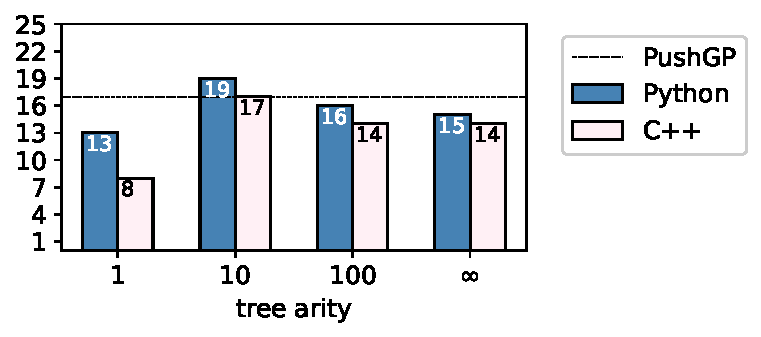
\includegraphics[width=0.5\linewidth, trim={0mm 2.8mm 0mm 2mm}, clip]{images/num_solved_problems_vs_bf_1000_v3_zenodo.pdf}
  %
  % % \vspace*{-2mm}
  \caption{Number of solved PSB2 problems depending on tree arity in beam search for prompt type \ref{seidr:prompt-0}.}
  \label{fig:seidr:solved-vs-bf}
\end{figure}

The results highlight the benefit of compromise strategies with tree arity of 10 and 100 over repair-only ($N=1$) and replace-only ($N=\infty$) strategies. 
The results show that the repair-only scheme is outperformed by other strategies. 
We explain the poor performance of the repair-only strategy by the fact that the search space is under-explored. 
Specifically, the replace scenario ensures that the LLM for the debugging component represented by Codex-edit in our experiments generates different updates of program candidates using variable temperatures.
The probability of finding a better fix is higher when more alternatives are generated to update the draft program at $N>1$ compared to $N=1$. 
The search strategy with $N=10$ yields the best results: it performs on par with PushGP for C++ and outperforms the baseline during Python program synthesis by +2 problems, resulting in a total of 19 programs that pass all test cases.
The results imply that generating a moderate number of programs in parallel during the DEBUG step works better than the policies in which more updates are generated for each program (100 or 1000), 
or those in which only one program is updated iteratively.

We present the analogy of the solution speed for all four arities and the fixed default debug instruction in Figure~\ref{fig:seidr:epg-distribution}. 
In detail, we show the distribution of EPG values in all experiments to explore how many candidate updates are generated before the solution is found.
We zoom in to the cases with solutions found with up to the first 10 program candidates in Figure~\ref{fig:seidr:epg-distrib-solved-10} and show the EPG distribution with the step of 100 candidates in Figure~\ref{fig:seidr:epg-distrib-solved-100}. 
In addition, we break down the results into each tree arity in Figure~\ref{fig:seidr:epg-bf}, showing the EPG on a heatmap scale and the TPR as a number between 0 and 1, or the signs ``+'' if a problem is solved and ``-'' if the final TPR is 0. 


\begin{figure}[t]
 %
\begin{subfigure}[t]{\columnwidth}
\centering
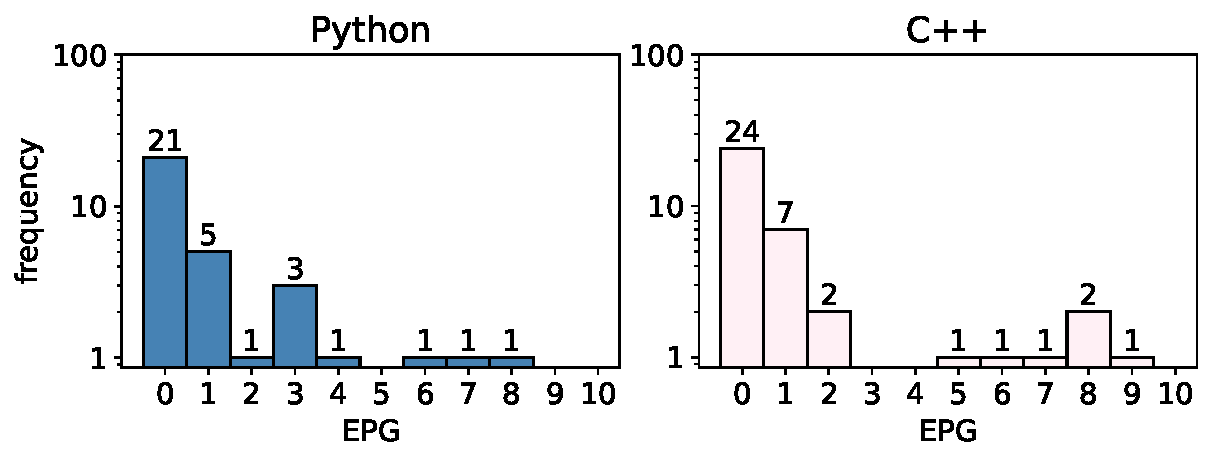
\includegraphics[width=.7\linewidth, trim={0mm 4mm 0mm 0mm}]{images/epg_distribution_solved_maxprog_1000_1_v3_zenodo.pdf}
  \caption{0 $\leq$ EPG $\leq$ 10 with step 1.}
  \label{fig:seidr:epg-distrib-solved-10}
\end{subfigure}

% \vspace{2mm}

\begin{subfigure}[t]{\columnwidth}
\centering
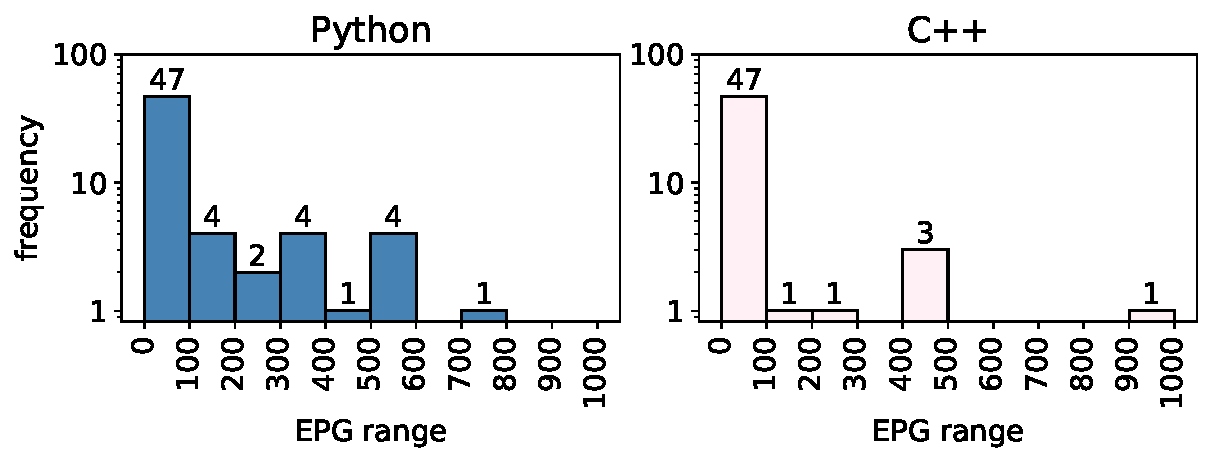
\includegraphics[width=.7\linewidth, trim={0mm 4mm 0mm 0mm}]{images/epg_distribution_solved_maxprog_1000_100_v3_zenodo.pdf}
  \caption{0 $\leq$ EPG $\leq$ 1000 with step 100.}
  \label{fig:seidr:epg-distrib-solved-100}
\end{subfigure}
% % \vspace{-2mm}
\caption{Distribution of the number of generated programs during each problem-solving attempt in the experiments with different tree arities where a problem solution is found.}
\label{fig:seidr:epg-distribution}
\end{figure}

\begin{figure}[t]
  \centering
  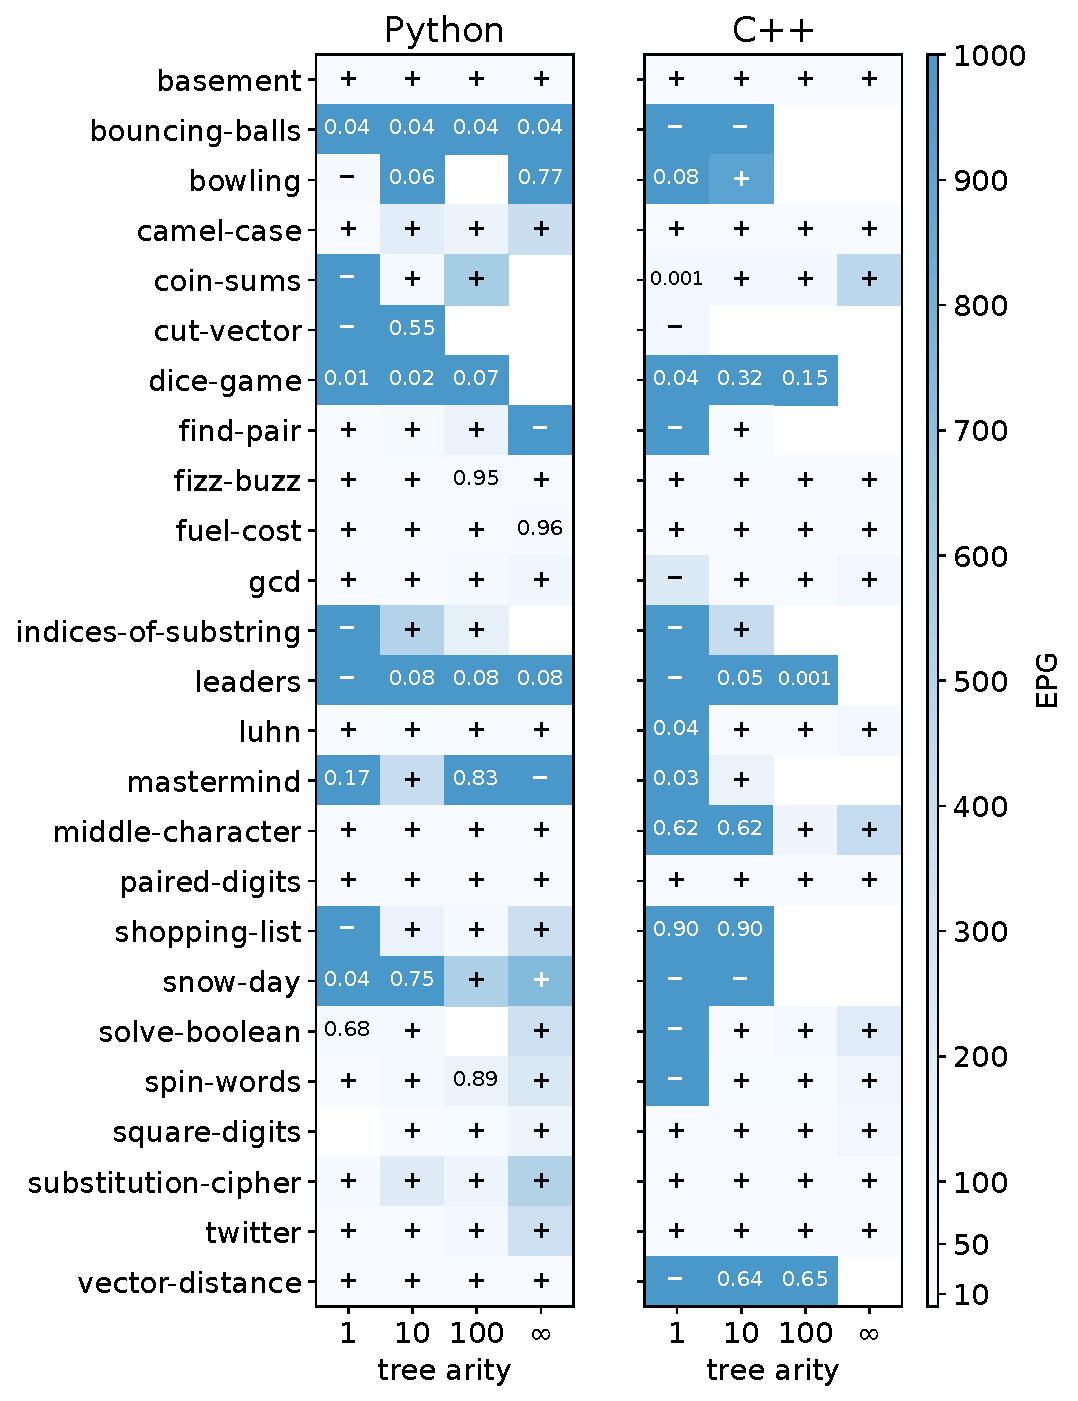
\includegraphics[width=.56\textwidth, trim={3mm 1.6mm 3mm 2mm}, clip]{images/num_programs_generated_vs_bf_test_pass_rate_vertical_maxprog_1000_v3.pdf}
  \caption{Number of excess programs generated (in color) and test pass rate (as numbers) depending on tree arity. Higher EPG values are shown in darker shades. We denote solved problems with ``+'' (test pass rate = 1), unsolved problems with ``-'' (test pass rate = 0), and show the test pass rate for partially solved problems. }
  \label{fig:seidr:epg-bf}
\end{figure}

Out of 100 experiments for each language, in 21--24\% of runs in Python and C++, the draft program is already the solution (EPG=0). 
For 31--33\% of the experiments, the solution is found after discarding 5 candidates. 
Around half of the experiments do not generate more than 100 programs. 
However, 5 problems are solved with more than 500 generated programs in Python and 1 problem in C++ (with $N=10$).
The results imply that the first steps in updating the draft program are crucial for solving the problem. 
The chances of solving the problem in later stages of the search, such as after 100 programs have been generated, are low.
This confirms our initial assumption in Section~\ref{sec:seidr-trade-off-settings} that 1000 programs are sufficient.

To briefly analyze Figure~\ref{fig:seidr:epg-bf}, we observe that some problems are solved in both languages, whereas some others --- only in Python. 
In addition, only five problems are not solved in any SEIDR configuration in Python (bouncing-balls, bowling, cut-vector, dice-game and leaders) and seven in C++ (bouncing-balls, cut-vector, dice-game,  leaders, shopping-list, snow-day, and vector-distance).
Upon closer inspection of generated programs, we have noticed that in bouncing-balls, the programs have logical errors and differ considerably between programming languages, as well as in the majority of unsolved problems. 
Test cases and debug instructions in bowling frequently skewed the resulting programs to return answers to individual bowling score strings instead of writing an algorithm to calculate the score based on each next character.
The latter mistake happened in other unresolved problems, such as cut-vector.
Qualitative analysis has also shown that some programs failed to read input from the user and instead defined input strings within the code, which limited the program to testing only one I/O pair, although the algorithm was correct.


\begin{highlight}
\textbf{Repair-replace trade-off in the initial exploration (\rqtreearity{}):} 
SEIDR with Codex as the coding LLM outperforms the PushGP baseline on PSB2 in Python and performs on par with it in C++ experiments with tree arity of 10. 
Search strategies with tree arity larger than one benefit from the replace possibility of the SEIDR framework as a consequence of using variable temperature for Codex-edit.
The repair component is also crucial for the framework because the replace-only search policy (with tree arity of $\infty$) performs worse than the policies that alternate between replace and repair during the program update (with tree arity of 10 or 100).  
\end{highlight} 


\subsection{Generalizability Experiments}

In this section, we present and discuss replace-repair trade-off results obtained with GPT-3.5 and Llama 3 and the effect of switching from tournament selection to lexicase selection with the best hyperparameter settings found for the trade-off. 
We count the number of fully solved problems (i.e., reached $TPR=1$) in experiments with the hyperparameter settings described in Table~\ref{tab:w-n-generalizability} in six runs and present the language-specific results for PSB2 and HumanEval.
% in Figure~\ref{fig:repair-replace-trade-off-generalizability}. 
We also explore the total number of programs that need to be generated before a solution is obtained, as well as
% in Figure~\ref{fig:epg-distribution} 
in how many of the six runs each problem is fully solved.
% in Figures~\ref{fig:epg-num-solved-psb2},~\ref{fig:epg-num-solved-he-python}, and~\ref{fig:epg-num-solved-he-c++}. 
The figures are described in detail in the dedicated sections. 

\subsubsection{Repair-replace Trade-off and Robustness to Restarts in the Generalizability Experiments.}
\label{sec:seidr-treearity-ollama}\label{sec:seidr-results-rqllama}

We compare the number of solved problems in the experiments with $\treearity_\text{draft}=\treearity_\text{debug}$ values of 1, 2, 4, 10, 16, $\infty$ (100) and $\treearity_\text{explain}=2$ in Python and C++ and tournament selection ranking strategy in Figure~\ref{fig:repair-replace-trade-off-generalizability}. 
We will refer to the equally set values of $\treearity_\text{draft}$ and $\treearity_\text{debug}$ as $N^*$ hereafter.
As before, experiments with $N^*=1$ and $N^*=\infty$ correspond to ablation studies, where the replace option or the repair option is turned off. 
The results of SEIDR are compared to the baseline performance of PushGP on the PSB2 benchmark, which solves 17 out of 25 problems. 
The boxplots show the inter-quartile range between the first and third quartiles observed in six runs and the median values as horizontal lines within the boxes. 

%%%%%%%%%%%%%%%%%%%%%%%%%%%%%%%%%%%%%%%%%%
% Num solved problems
%%%%%%%%%%%%%%%%%%%%%%%%%%%%%%%%%%%%%%%%%%
\begin{figure}[bt]
\begin{subfigure}{\linewidth}
\centering
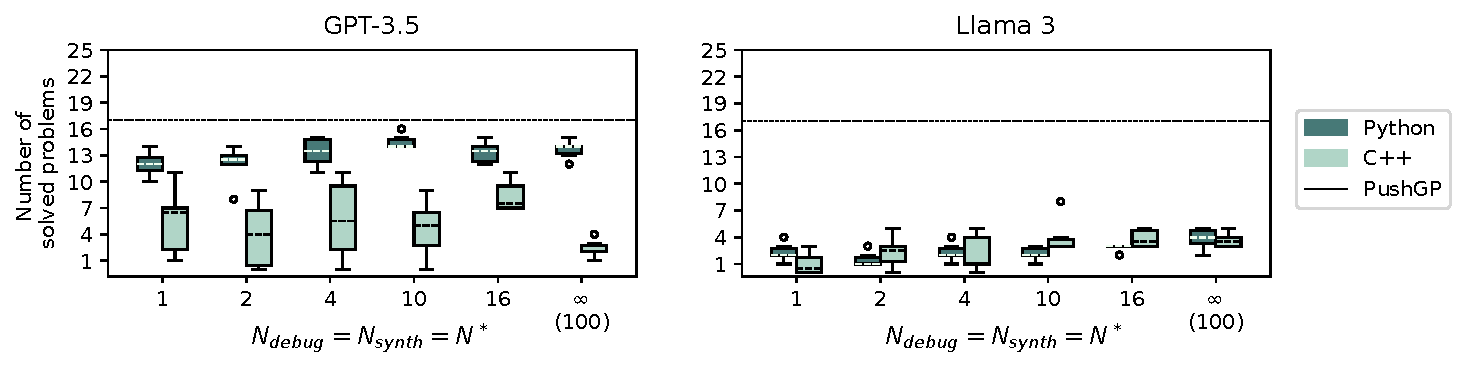
\includegraphics[width=\linewidth, trim={0mm 0mm 0mm 0mm}]{images/num_solved_problem_psb2_6runs_boxplot_v5.pdf}
%\vspace{-15pt}
  \caption{PSB2}
  \label{fig:num-solved-psb2-gpt3.5}
\end{subfigure}
\begin{subfigure}{\columnwidth}
\centering
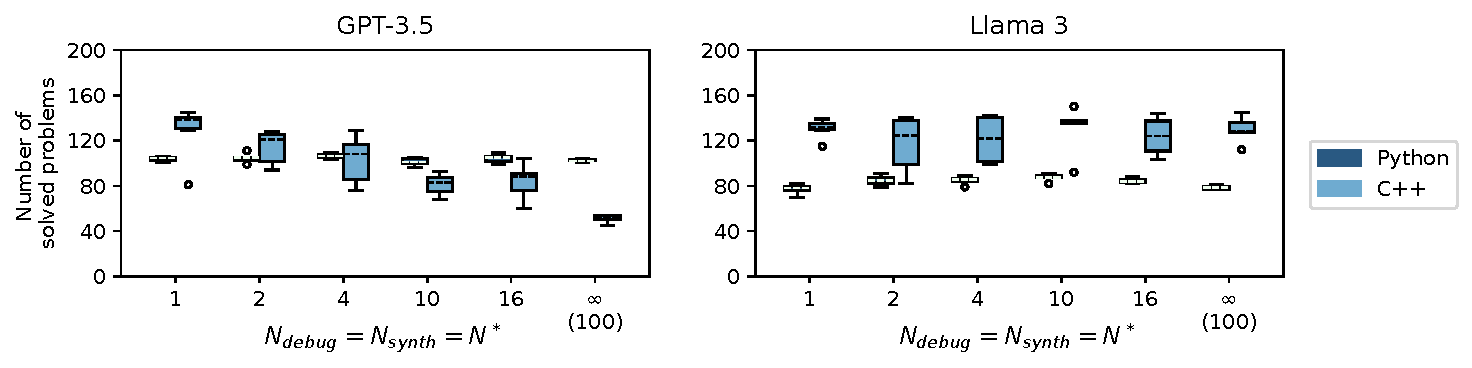
\includegraphics[width=\linewidth, trim={0mm 0mm 0mm 0mm}]{images/num_solved_problem_humaneval_6runs_boxplot_v5.pdf}
%\vspace{-15pt}
  \caption{HumanEval}
  \label{fig:num-solved-he-gpt3.5}
\end{subfigure}
%\vspace{-16pt}
\caption{Repair-replace trade-off as a tree search problem in SEIDR: the total number of solved problems as measured by $TPR=1$ using SEIDR with GPT-3.5 and Llama 3 depending on tree arity $N^*$.}
\label{fig:repair-replace-trade-off-generalizability}
\end{figure}


The trend present for all the datasets and models is that the results for Python are more condensed over six runs than for C++. 
Since access to statistics about the training data for Llama 3 and GPT-3.5 is not provided, reasons for more stable performance in Python across runs can possibly lie in the training data distribution but cannot be confirmed. 
However, the fact that HumanEval-Python is a popular code generation benchmark against which models are compared may affect the results on this and other Python benchmarks.
In the same line of comparison of results between two programming languages, SEIDR with GPT-3.5 performs better in Python than in C++ on PSB2. 

% In the majority of experiments, based on the number of fully solved problems, it is beneficial to use the tree arity larger than 1 and less than $\infty, $ except for GPT-3.5 on HumanEval-C++. 
% This result confirms that, for the majority of cases, using SEIDR that builds a tree of solutions is better than repairing only one program or regenerating the program from scratch every time. 
% 
Llama~3 performs worse than GPT-3.5 on PSB2 in both languages.
This dataset has more test cases in stock than HumanEval and can be considered a more thorough test of the coding and debugging capabilities of LLMs. 
Following a recent trend, where larger models outperform smaller ones, the results of SEIDR on PSB2 confirm that the smaller model (Llama~3) performs worse than the larger one (GPT-3.5).

Looking back at the initial experiments with Codex and PSB2, we notice the degradation of performance from Codex to GPT-3.5: SEIDR with Codex solved 19 problems in Python and 17 in C++ with tree arity 10, while the best-performing result of SEIDR GPT-3.5 is 16 (tree arity of 10, too) in Python and 11 in C++ (several tree arities, but not 10). 
This result can be explained by the focus of LLM builders on the generalization of knowledge and performance on a variety of tasks, while Codex specializes in code generation.
Moreover, due to increased costs from Codex to GPT-3.5, we decrease the maximum number of generated program candidates from 1000 for Codex to 100 for GPT-3.5. 
However, only two problems are solved with Codex with $EPG > 100$: indices of substring (at program candidate \#510) and substitution cipher (at candidate \#210) in Python, bowling (candidate \#912) and indices of substring (\#410) in C++. 
Meanwhile, some problems are solved by Codex earlier than at the debugging attempt \#100 and not solved by GPT-3.5 and vice versa. 
Therefore, the reduction of the maximum generated programs has only a partial effect on the difference between the results of the two models. 


\begin{figure}[bt]
\begin{subfigure}{\linewidth}
\centering
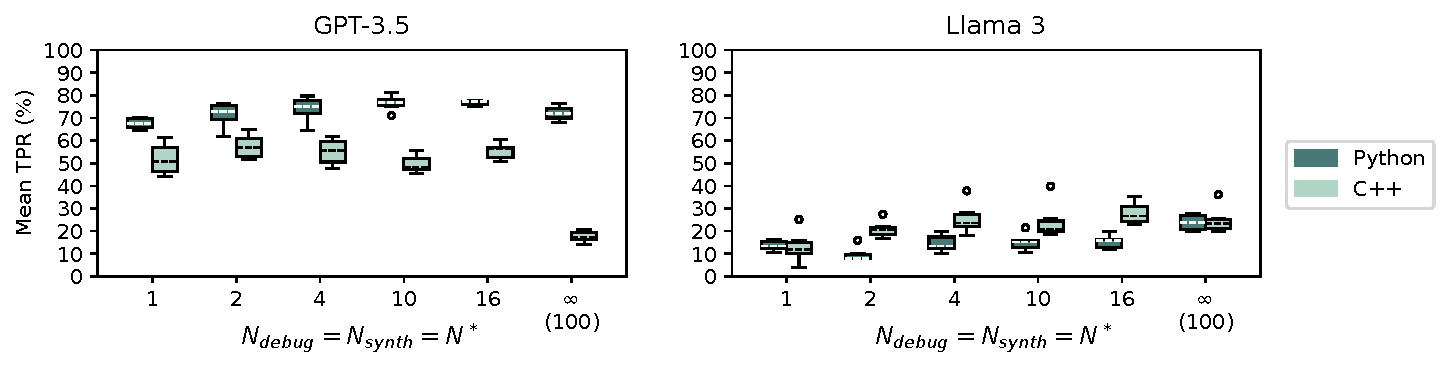
\includegraphics[width=\linewidth, trim={0mm 0mm 0mm 0mm}]{images/mean_tpr_psb2_6runs_boxplot_v5.pdf}
%\vspace{-15pt}
  \caption{PSB2}
  \label{fig:mean-tpr-psb2-gpt3.5}
\end{subfigure}
\begin{subfigure}{\columnwidth}
\centering
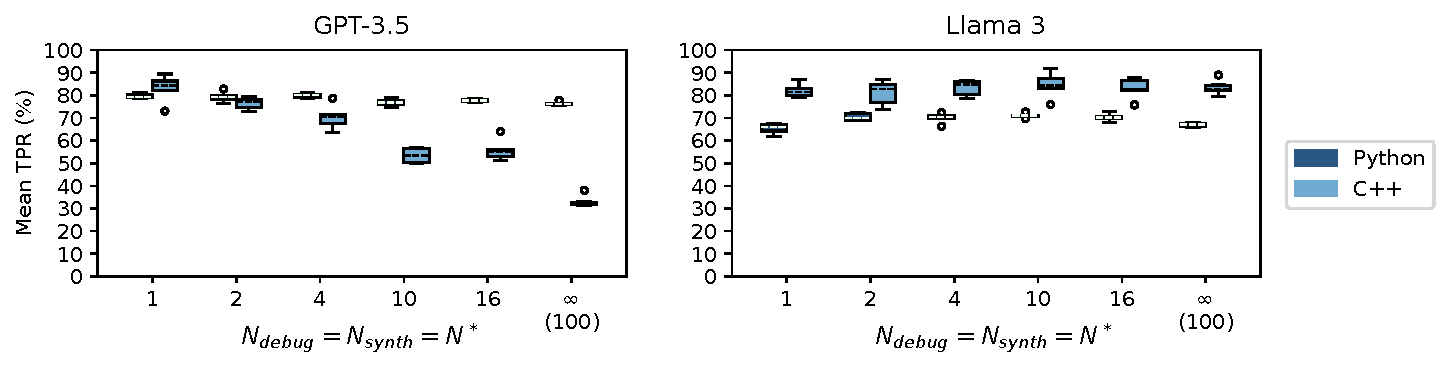
\includegraphics[width=\linewidth, trim={0mm 0mm 0mm 0mm}]{images/mean_tpr_humaneval_6runs_boxplot_v5.pdf}
%\vspace{-15pt}
  \caption{HumanEval}
  \label{fig:mean-tpr-he-gpt3.5}
\end{subfigure}
%\vspace{-16pt}
\caption{Repair-replace trade-off as a tree search problem in SEIDR: mean $TPR$ measured in \% obtained using SEIDR with GPT-3.5 and Llama 3 depending on tree arity $N^*$.}
\label{fig:mean-tpr-repair-replace-trade-off-generalizability}
\end{figure}


In addition to reporting the number of fully solved problems, Figure~\ref{fig:mean-tpr-repair-replace-trade-off-generalizability} also reports the mean Test Pass Rate measured in \%. 
For HumanEval-C++, SEIDR with GPT-3.5 has better results with smaller tree arity values than with larger ones.
In Python, experiments with $1 < N^* < 100$ (i.e., non-corner case values of $N^*$) yield better mean TPR for SEIDR with GPT-3.5 on PSB2 and with Llama~3 --- for HumanEval-Python.
SEIDR with Llama~3 performs with slightly better mean TPR towards larger $N^*$  on PSB2-C++, and at the same time, it performs well on HumanEval-C++, so the difference between results with different $N^*$ is small.
The maximum of mean TPR for both datasets and models and max number of solved problems are obtained with $N^*=16$ or less, except for Llama 3 in PSB2-C++. 
From this part of the experiments, we notice that moderate or small tree arities $(N^* \le 16)$ are preferred, but there is no one leading tree arity.


The number of runs in which a problem is solved and the average speed of finding those solutions are shown in Figure~\ref{fig:epg-num-solved-psb2} for PSB2, Figure~\ref{fig:epg-num-solved-he-python}
for HumanEval-Python and Figure~\ref{fig:epg-num-solved-he-c++} for HumanEval-C++.
These figures show which problems were not solved in any run of any experiment (a row with zeros colored white) and what problems are easier to solve than others (e.g., solved in all runs, or at least one with each tree arity $N^*,$ or earlier in the search tree and shown in brighter rather than darker color but not white). 
We also show the results of lexicase selection runs marked with ``lex.'' in these three figures, but will discuss them in a separate section. 

The majority of solved PSB2 problems are solved in more than one run per setting with GPT-3.5 and faster (with fewer attempts) in Python than in C++ as illustrated in Figure~\ref{fig:epg-num-solved-psb2}.
For Llama~3, most of the solutions are obtained in 1--3 runs.
The trend for both datasets is that, for problems where a solution is found, SEIDR with GPT-3.5 makes fewer attempts in Python (brighter colors prevail in the corresponding parts of Figures~\ref{fig:epg-num-solved-psb2} and~\ref{fig:epg-num-solved-he-python}) than SEIDR with GPT-3.5 in C++ or SEIDR with Llama~3 in both languages (darker shades in the GPT-3.5 on C++ and Llama~3 parts of Figures~\ref{fig:epg-num-solved-psb2} and \ref{fig:epg-num-solved-he-c++}).


\begin{figure}[tb]
  \centering
  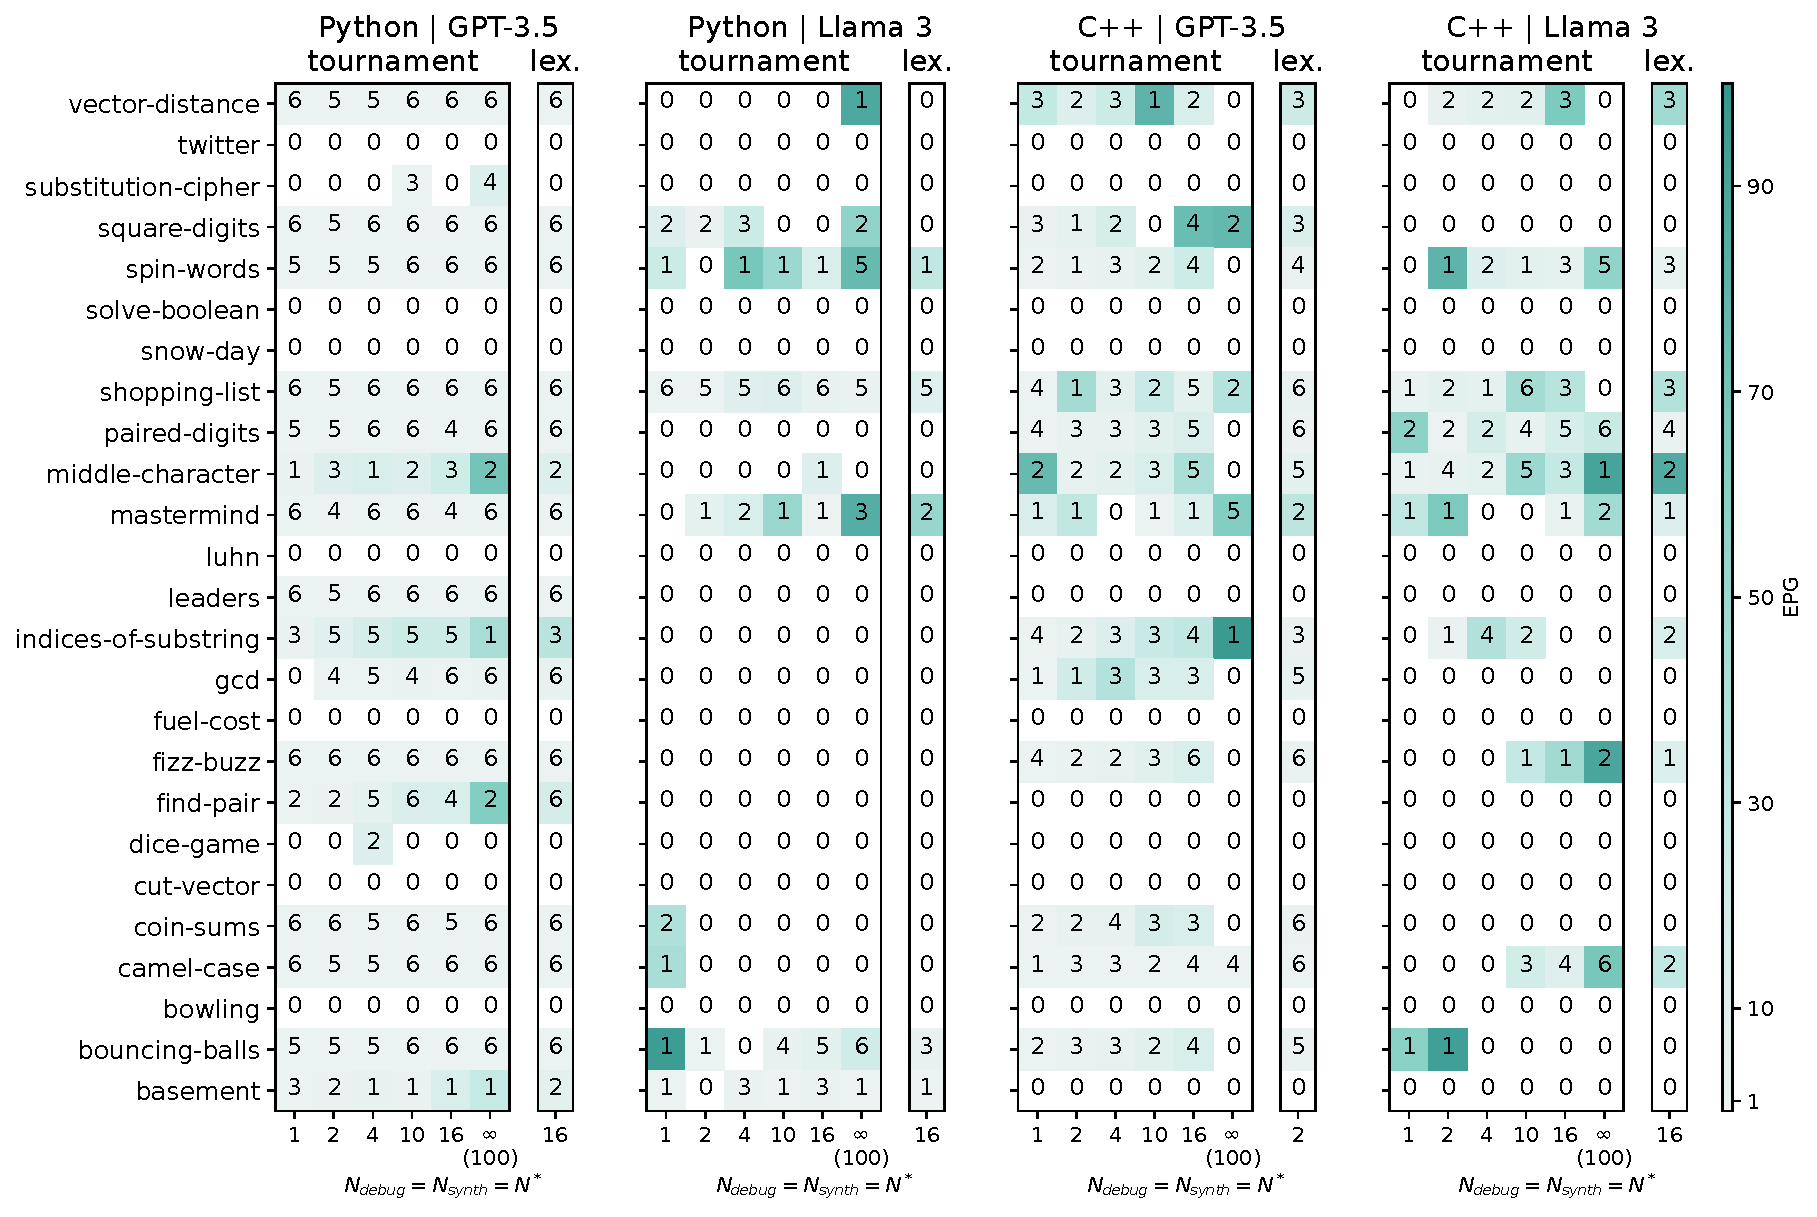
\includegraphics[width=\linewidth, trim={3mm 2.8mm 3mm 2mm}, clip]{images/epg_mean_and_num_runs_problem_solved_avg_score_check_w_lexicase_psb2_6runs_heatmap_v5.pdf}
  \caption{PSB2: mean Excess Programs Generated (in color) and the number of runs in which a task is solved. The experiments in which a specific problem is not solved in any run are shown in white.}
  \label{fig:epg-num-solved-psb2}
  %\vspace{-3ex}
\end{figure}

\begin{figure}[hbt!]
  \centering
  % {left bottom right top},
  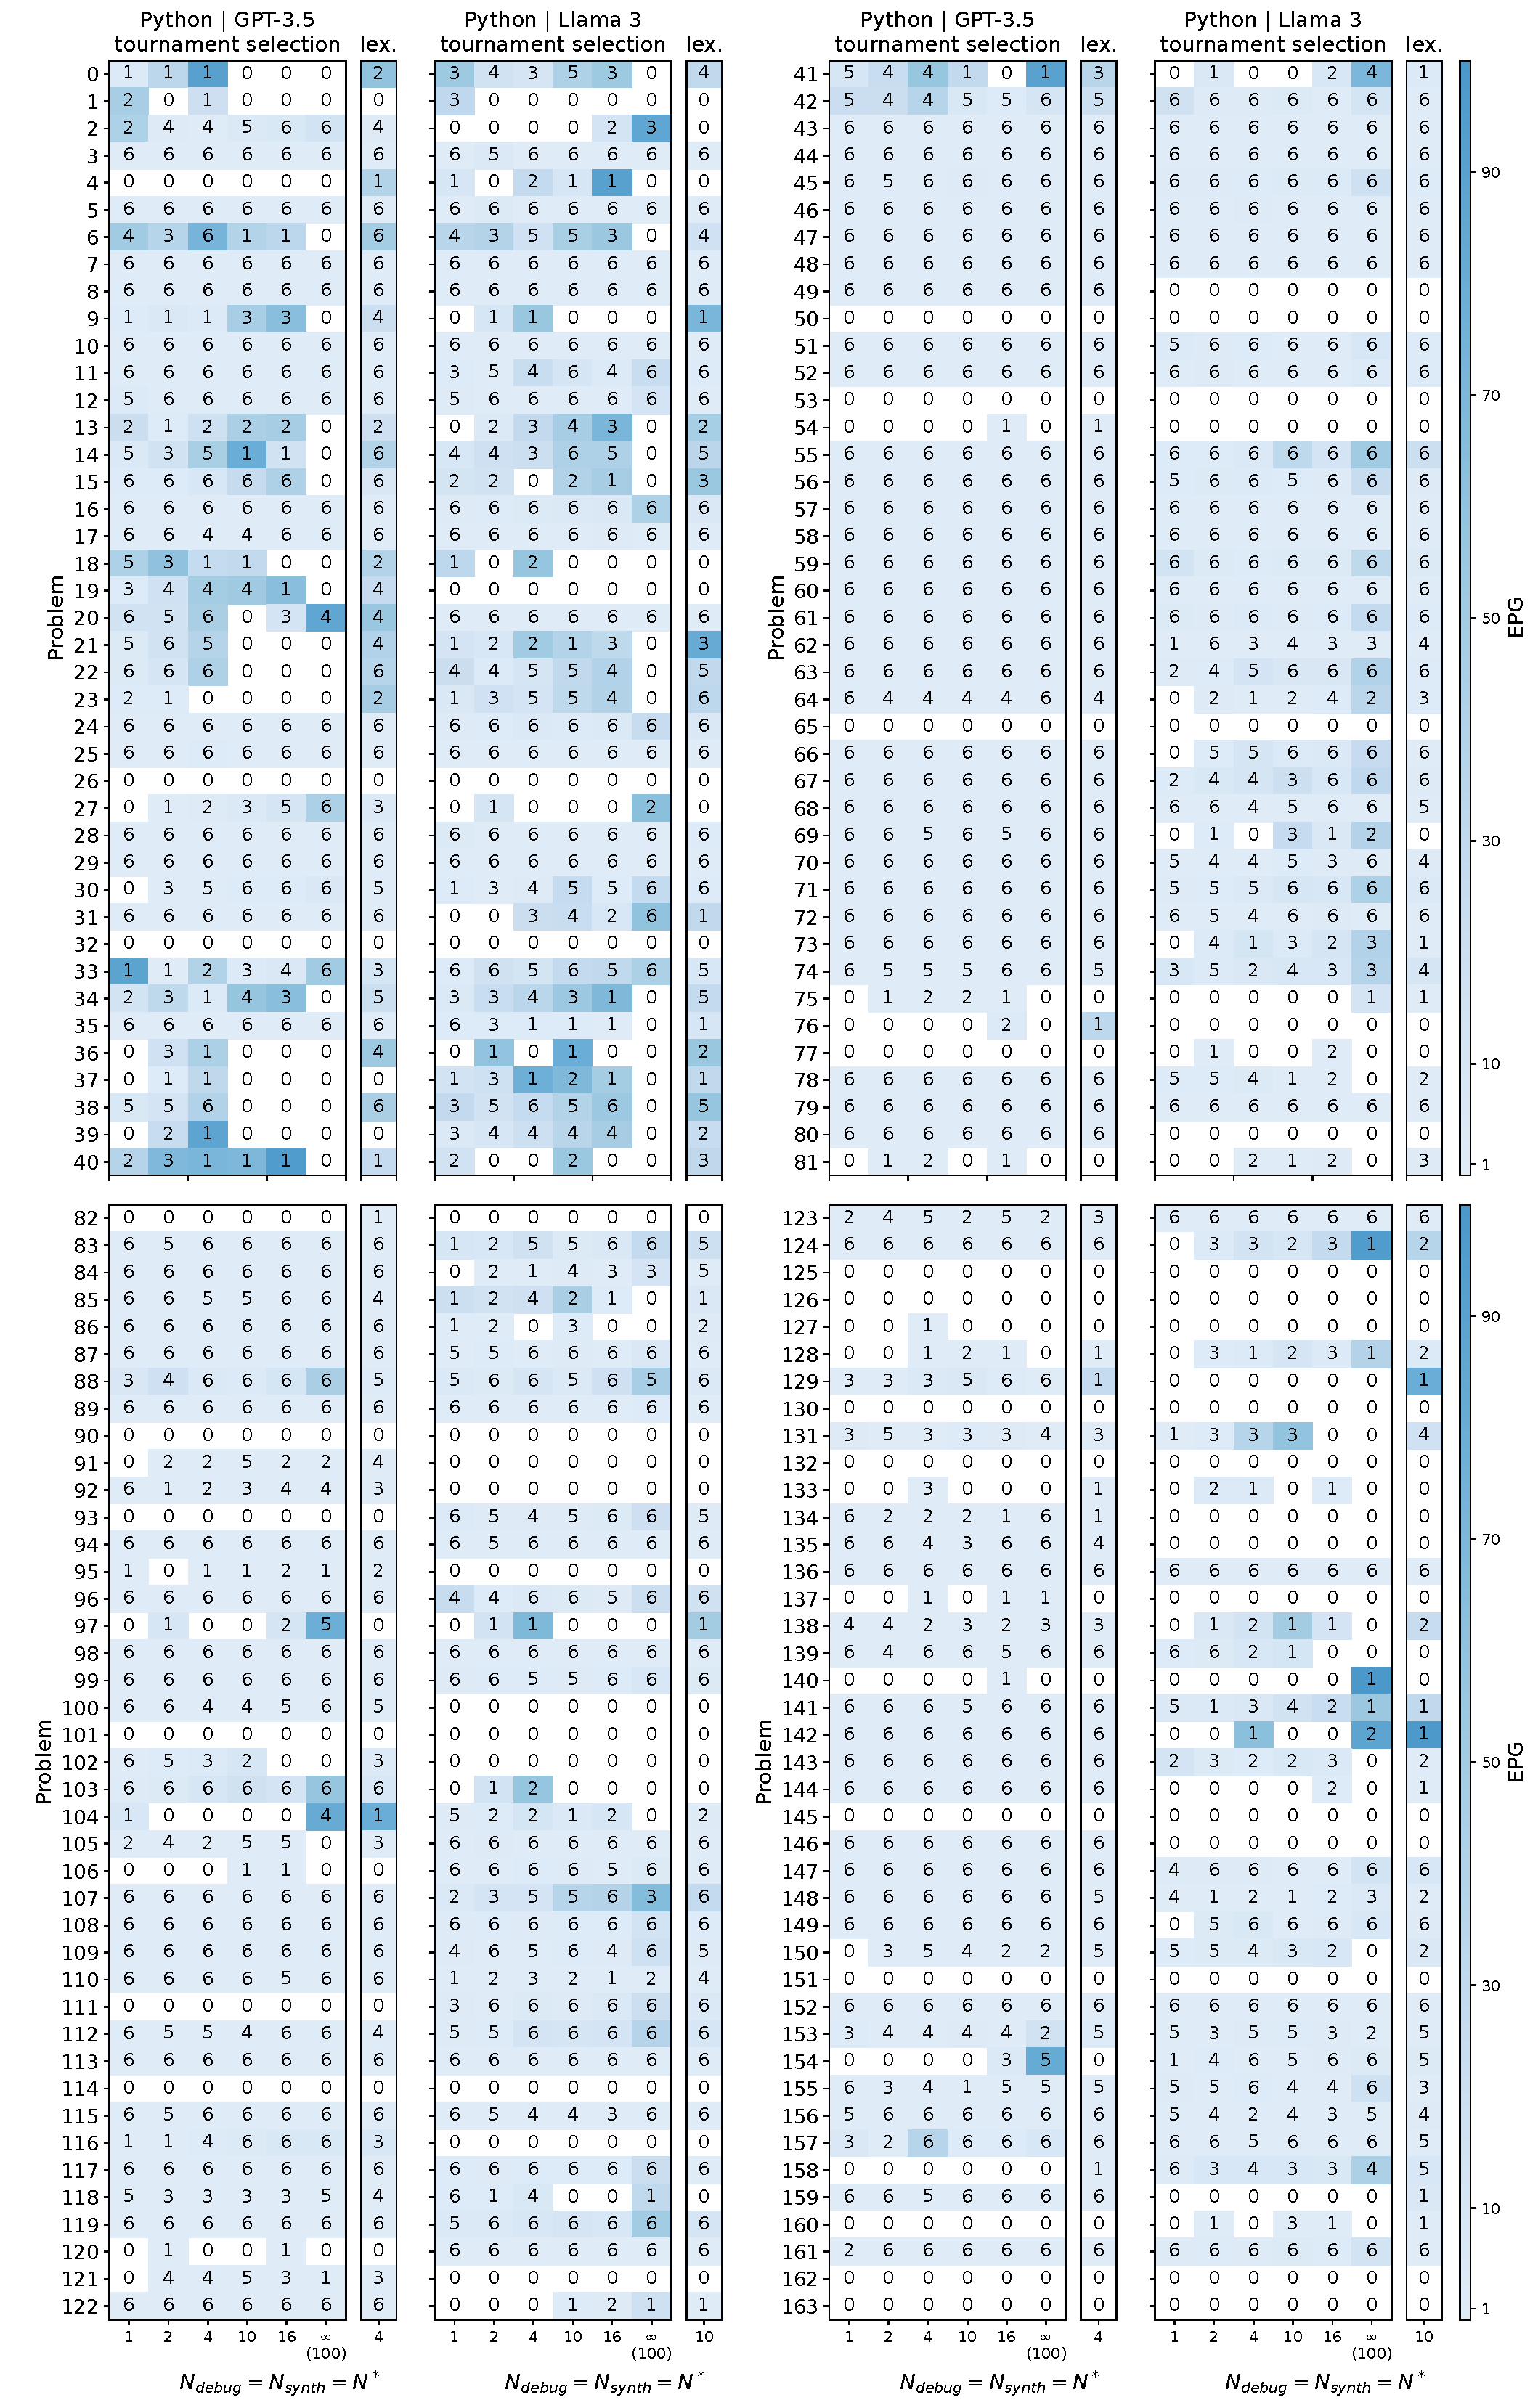
\includegraphics[width=.88\linewidth, trim={0mm 3mm 0mm 2.6mm}, clip]{images/epg_mean_and_num_runs_problem_solved_avg_score_check_w_lexicase_humaneval_Python_6runs_heatmap_v5.pdf}
  \vspace{-4pt}
  \caption{HumanEval-Python: mean Excess Programs Generated (in color) and the number of runs in which a task is solved. The problems that are not solved in any run are colored white.}
  \label{fig:epg-num-solved-he-python}
  \vspace{-12pt}
\end{figure}

\begin{figure}[hbt!]
  \centering
  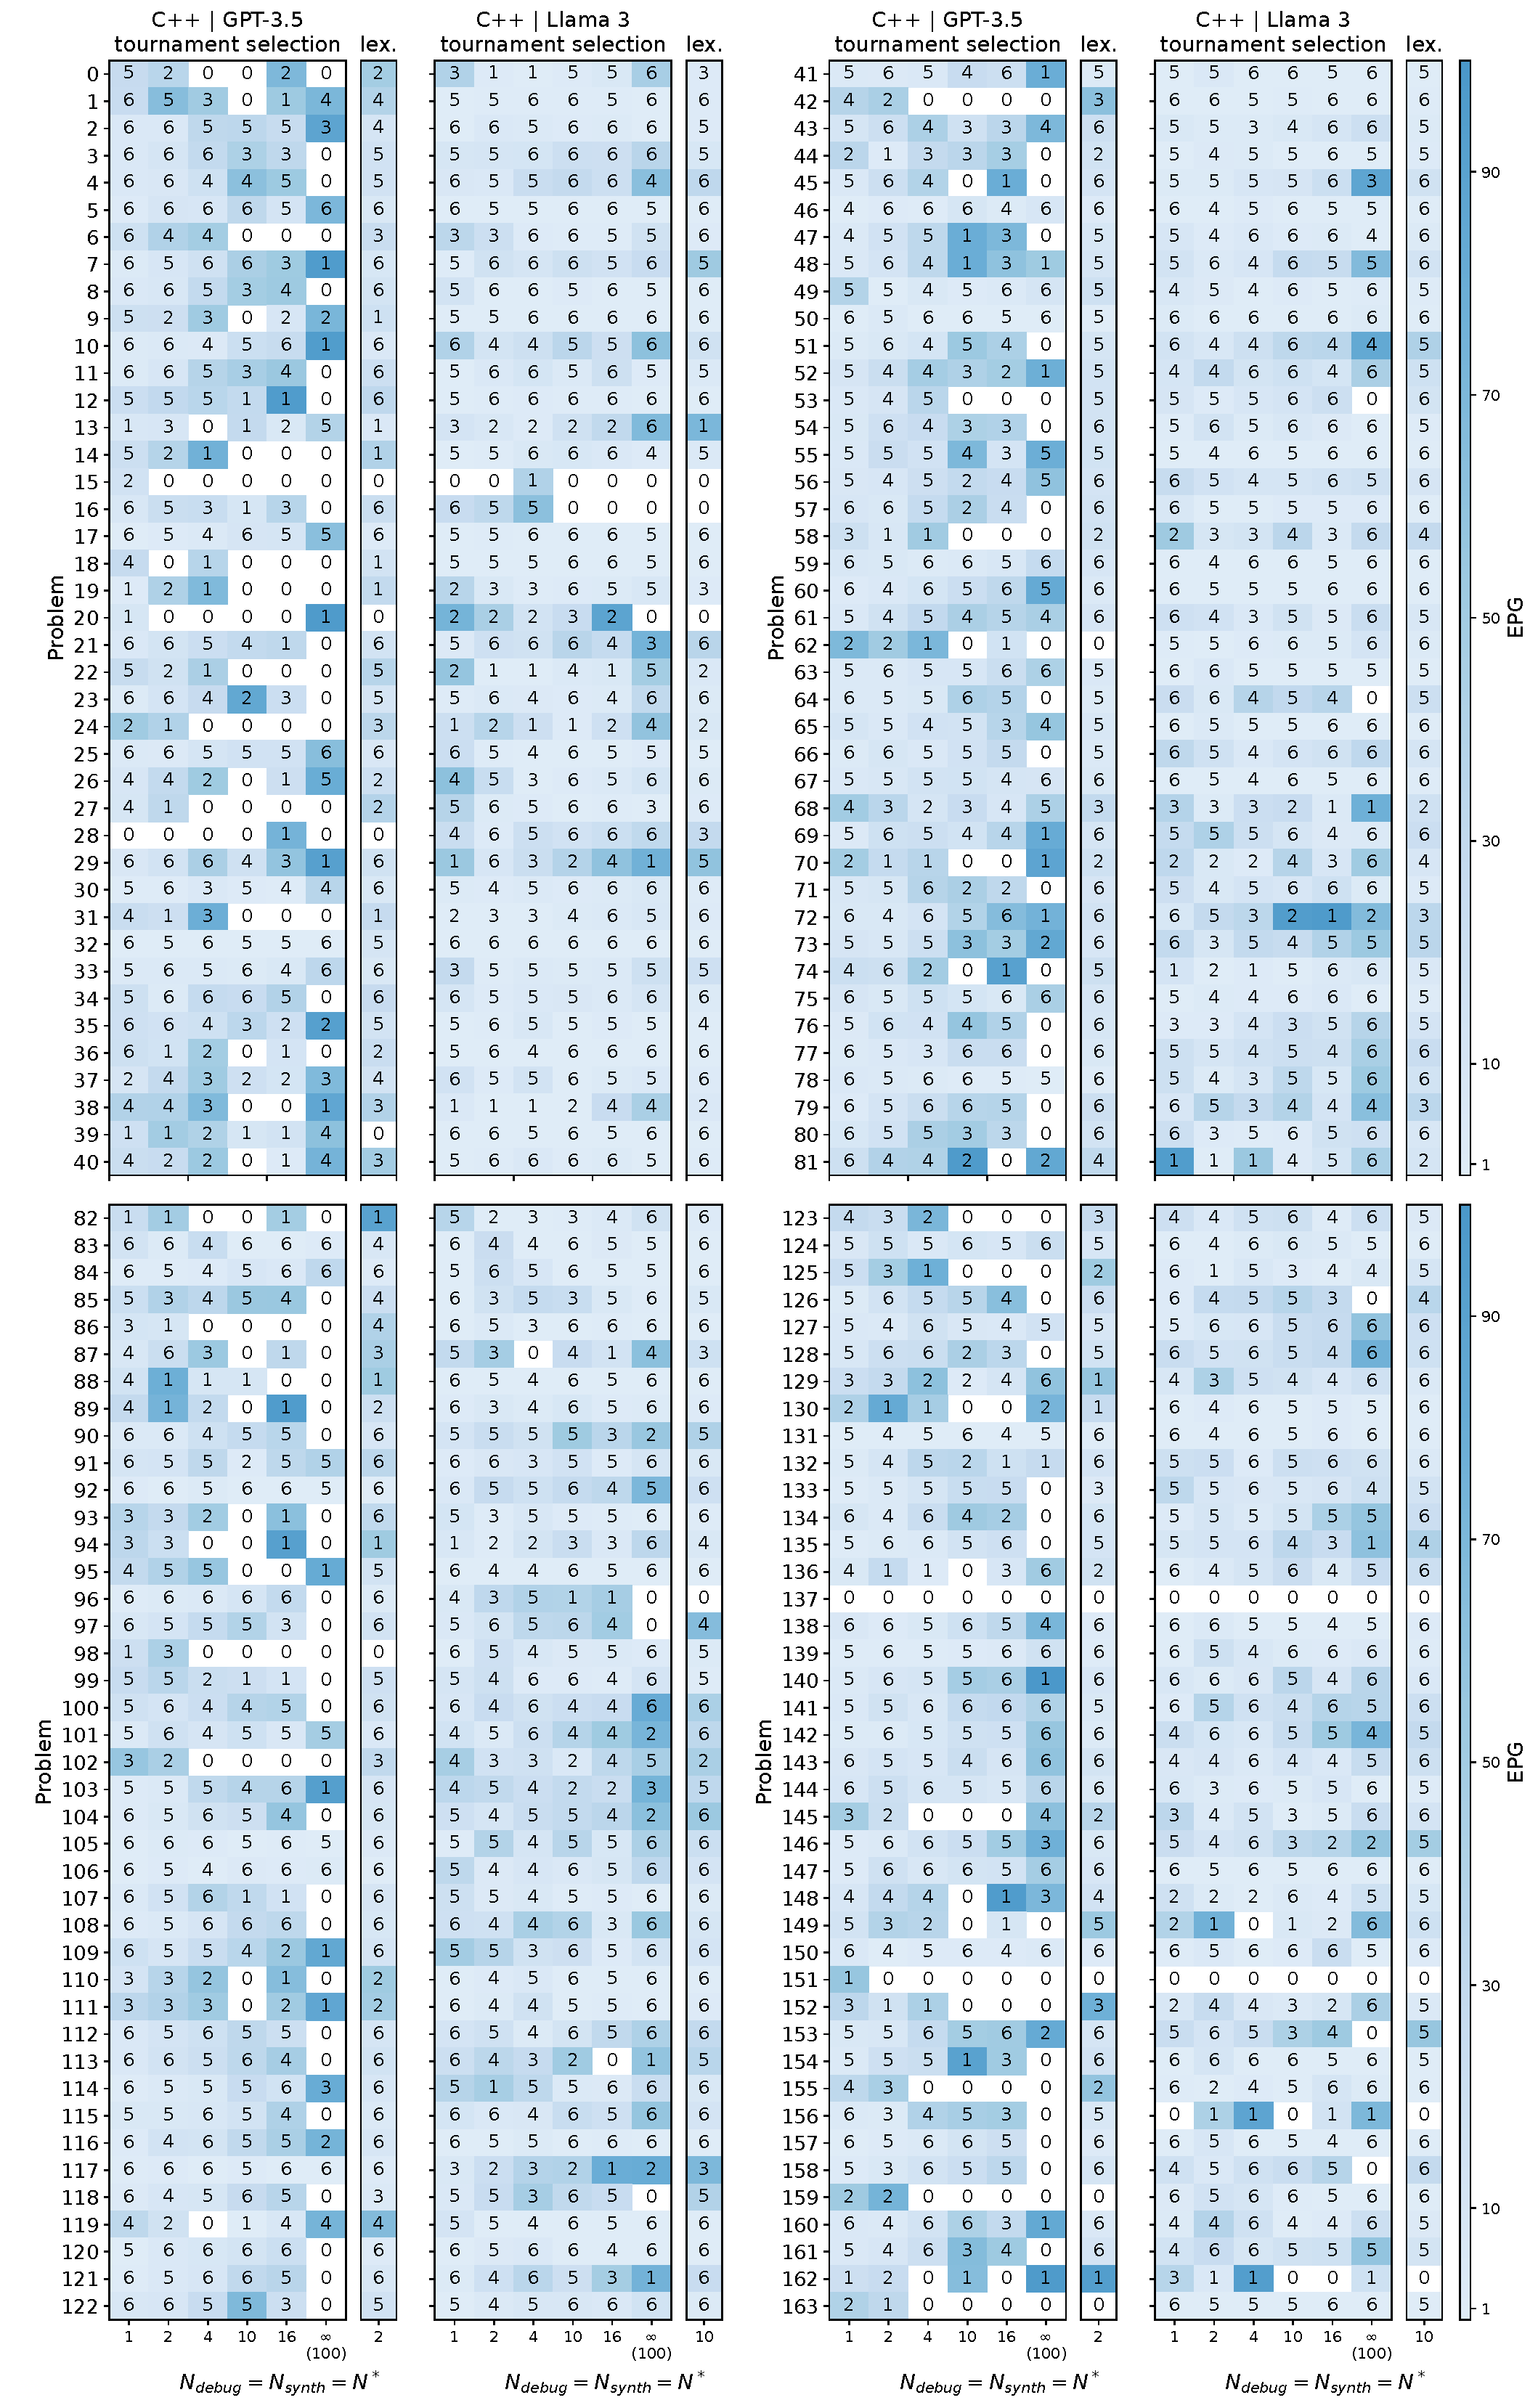
\includegraphics[width=.88\linewidth, trim={0mm 3mm 0mm 2.6mm}, clip]{images/epg_mean_and_num_runs_problem_solved_avg_score_check_w_lexicase_humaneval_C++_6runs_heatmap_v5.pdf}  %
  \vspace{-4pt}
  \caption{HumanEval-C++: mean Excess Programs Generated (in color) and the number of runs in which a task is solved. The problems that are not solved in any run are colored white.}
  \label{fig:epg-num-solved-he-c++}
  \vspace{-12pt}
\end{figure}


% Given resource constraints, such as the costs of calling GPT-3.5 and the time of running each experiment, we limit restarts to 6 runs in total with each set of hyperparameters.
% However, t

To explore the capabilities of SEIDR with the studied models, we can take a union over experiments and count the number of problems solved at least once across 36\footnote{~We have 6 runs and 6 different values of $N^*.$} restarts with a fixed dataset, language and model.
In this way, in addition to reporting the number of problems solved in each run in the boxplot, we can derive the number of problems solved in any run with any set of hyperparameter using information in Figures~\ref{fig:epg-num-solved-psb2}--\ref{fig:epg-num-solved-he-c++}.
For example, SEIDR with GPT-3.5 does not solve only 7 problems out of 25 PSB2-Python tasks (see Figure~\ref{fig:epg-num-solved-psb2}).
Namely, bouncing-balls, cut-vector, dice-game, indices-of-substring, middle-character, solve-boolean, and substitution-cipher are solved in 0 runs with all the variations of $N^*$.
% $=N_{synth}=N_{debug}.$
In other words, 18 unique problems are solved in the collection of all the experiments using SEIDR with GPT-3.5 on PSB2-Python. 
SEIDR with GPT-3.5 does not solve 12 out of 25 PSB2-C++ tasks with any hyperparameter settings. 
The number of solved problems in any run with SEIDR and Llama~3 are 10 for PSB2 in both languages. 
To support the finding about degradation of performance happening in a non-specialized model GPT-3.5 compared to the code-specialized Codex, we calculate the number of solved problems in any run with Codex and obtain 20 problems solved at least once in Python and 18 in C++. 

Similarly, SEIDR with GPT-3.5 solves 141 out of 164 HumanEval-Python problems at least once in all runs, collectively, and 128 problems with Llama~3 (see Figure~\ref{fig:epg-num-solved-he-python}).
In HumanEval-C++, SEIDR with GPT-3.5 solves 163 out of 164 problems (except CPP/137) in the union of all runs and 162 with Llama~3 (except CPP/137 and CPP/151) as follows from Figure~\ref{fig:epg-num-solved-he-c++}.


In Figure~\ref{fig:epg-distribution}, we present the analogy of the speed of obtaining solutions, EPG. 
We zoom in to the cases with solutions found with up to the first 10 program candidates in Figures~\ref{fig:psb2-epg-distrib-step-1} and~\ref{fig:humaneval-epg-distrib-step-1} for PSB2 and HumanEval-X, respectively. 
The coarser-grained EPG distribution with the step of 10 candidates is shown in Figures~\ref{fig:psb2-epg-distrib-step-10} and~\ref{fig:humaneval-epg-distrib-step-10}. 


% %%%%%%%%%%%%%%%%%%%%%%%%%%%%%%%%%%%%%%%%%%
% % EPG distribution
% %%%%%%%%%%%%%%%%%%%%%%%%%%%%%%%%%%%%%%%%%%
\begin{figure}[tb]
\begin{subfigure}{.8\columnwidth}
\centering
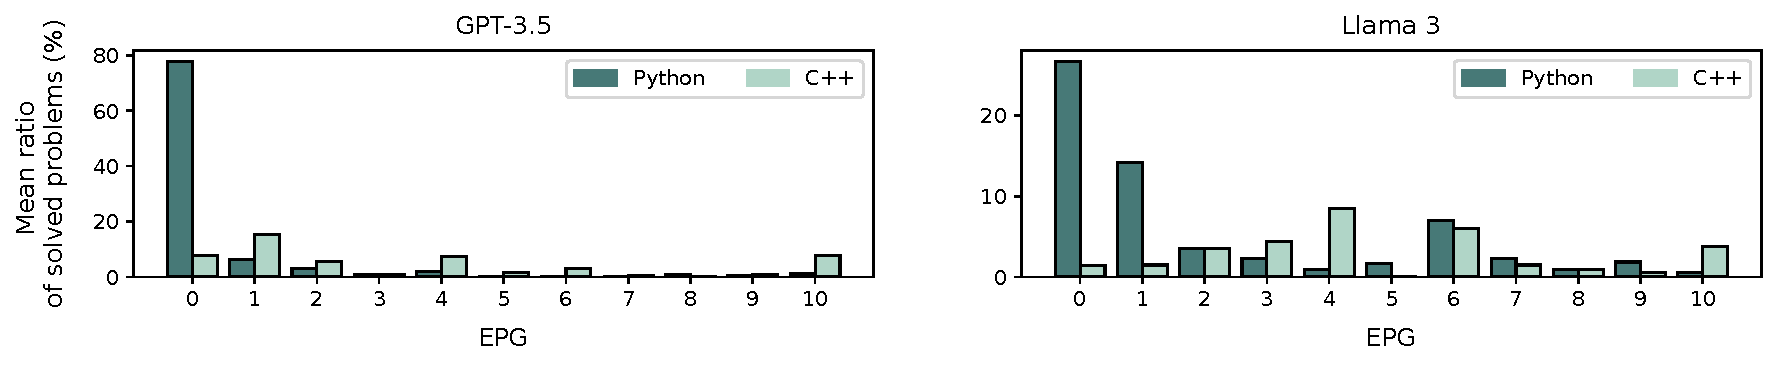
\includegraphics[width=\linewidth, trim={0mm 3mm 0mm 0mm}, clip]{images/epg_distribution_step_1_psb2_6runs_barplot_v5.pdf}
  \caption{PSB2: 0 $\leq$ EPG $\leq$ 10 with step 1.}
  \label{fig:psb2-epg-distrib-step-1}
\end{subfigure}
% 
% 
\begin{subfigure}{.8\columnwidth}
\centering
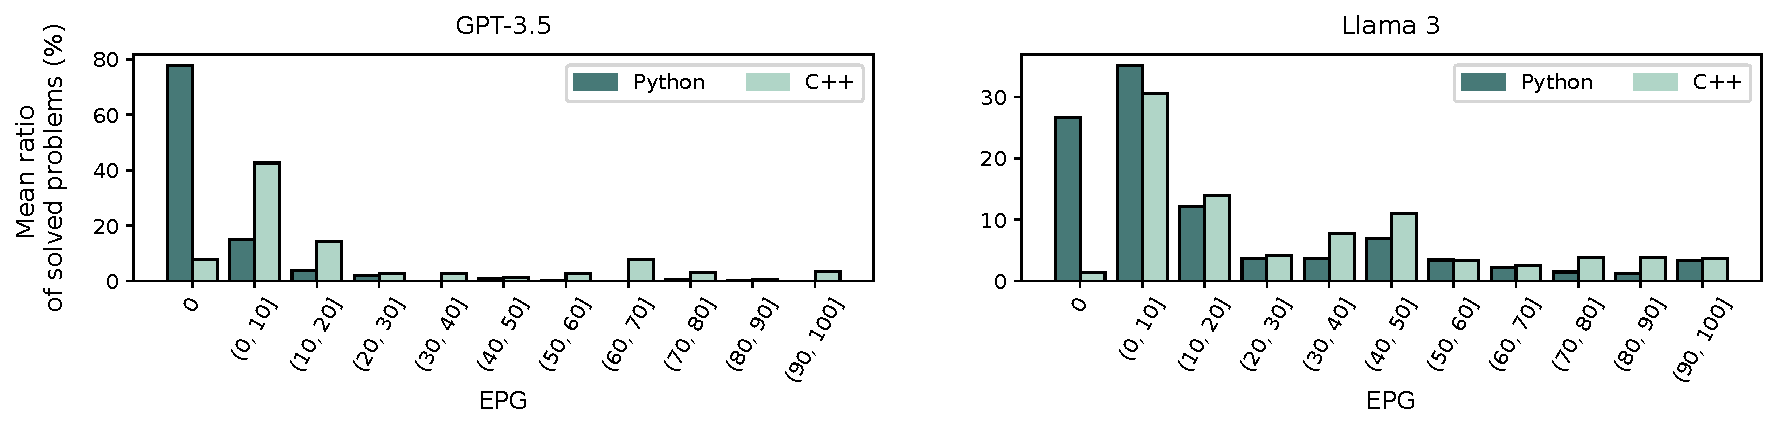
\includegraphics[width=\linewidth, trim={0mm 3mm 0mm 0mm}, clip]{images/epg_distribution_step_10_psb2_6runs_barplot_v5.pdf}
  \caption{PSB2: 0 $\leq$ EPG $\leq$ 100 with step 10.}
  \label{fig:psb2-epg-distrib-step-10}
\end{subfigure}
% 
\begin{subfigure}{.8\columnwidth}
\centering
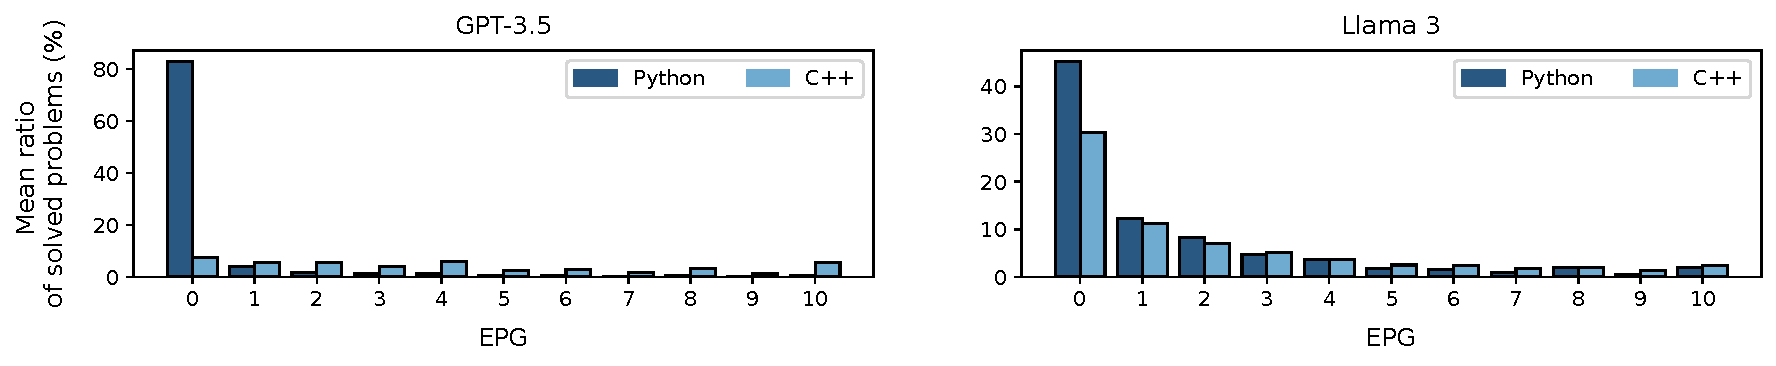
\includegraphics[width=\linewidth, trim={0mm 3mm 0mm 0mm}, clip]{images/epg_distribution_step_1_humaneval_6runs_barplot_v5.pdf}
  \caption{HumanEval: 0 $\leq$ EPG $\leq$ 10 with step 1.}
  \label{fig:humaneval-epg-distrib-step-1}
\end{subfigure}
% 
\begin{subfigure}{.8\columnwidth}
\centering
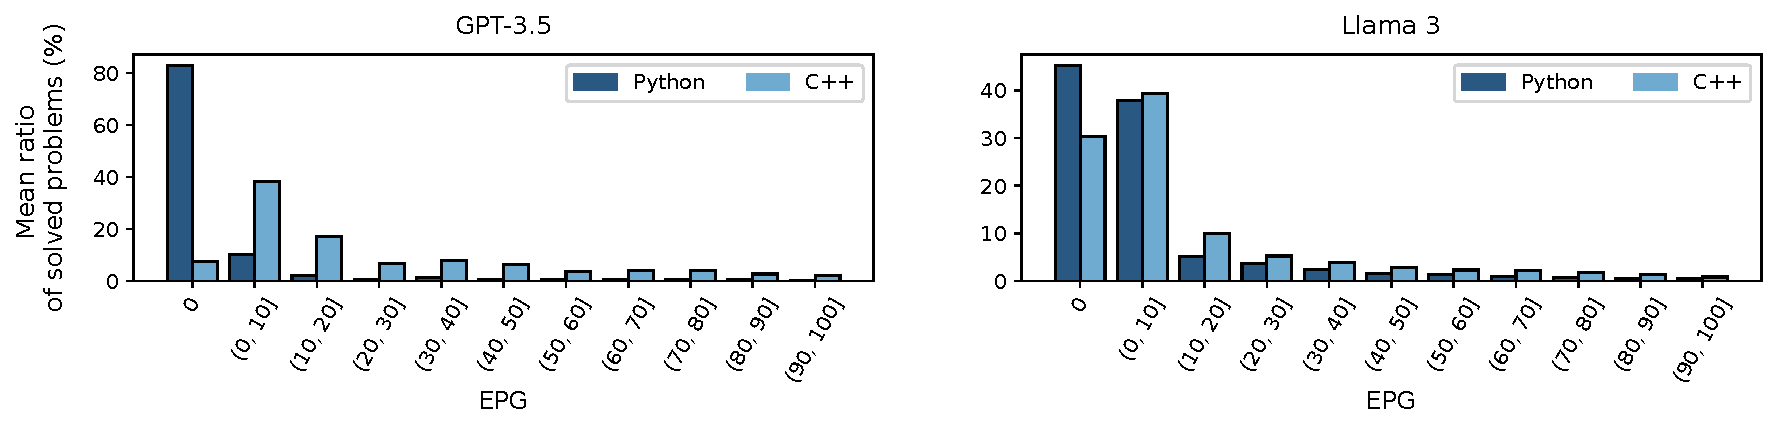
\includegraphics[width=\linewidth, trim={0mm 3mm 0mm 0mm}, clip]{images/epg_distribution_step_10_humaneval_6runs_barplot_v5.pdf}
  \caption{HumanEval: 0 $\leq$ EPG $\leq$ 100 with step 10.}
  \label{fig:humaneval-epg-distrib-step-10}
\end{subfigure}
\caption{Distribution (in \%) of the number of generated programs with GPT-3.5 and Llama 3 during each problem-solving attempt on average over 6 runs with different tree arities $\treearity_\text{draft}, \; \treearity_\text{debug}.$}
\label{fig:epg-distribution}
\end{figure}



In detail, we show the distribution of EPG values in all experiments to explore what proportion of candidate updates is made before a solution is found.
For example, on average, over 70\% of Python solutions by SEIDR with GPT-3.5 are solved from the first attempt, i.e., have EPG$=0$ (see Figure~\ref{fig:psb2-epg-distrib-step-1}).
Python solutions are more frequently found from the first attempt by SEIDR with Llama~3 than later in the tree, although less frequently than with GPT-3.5.
Most of solutions found by SEIDR benefit from the iterative repair and generate up to 10 extra programs with both models (see Figures~\ref{fig:psb2-epg-distrib-step-10}, \ref{fig:humaneval-epg-distrib-step-10}). 
However, some solutions are also found later in the tree search. 

The EPG distribution results for correctly solved problems with $TPR=1$ imply that the first steps in the update of the draft program are crucial for solving the problem. 
The chances of solving the problem in the later stages of the search are low.
This confirms our assumption in Section~\ref{sec:seidr-trade-off-settings} that 100 programs are sufficient in the generalizability experiments.

\begin{highlight}
\textbf{Repair-replace trade-off for SEIDR with GPT-3.5 and Llama~3 in the generalizability experiments (\rqtreearity{}, \rqllama{}, \rqmultirun{}):}
Unlike for SEIDR with Codex and a fixed debugging instruction (see Section~\ref{sec:seidr-seidr:rqtreearity}), SEIDR with GPT-3.5 and Llama~3 does not show any distinct trend for all the languages and datasets in terms of the preferred tree arity value. 
Results over a number of runs with the same hyperparameter settings are more condensed for Python than for C++, which can be a result of optimizing LLMs for high performance on popular coding benchmarks in Python.
If solutions to problems are found by SEIDR, it is done at an earlier tree search step for Python than for C++ (i.e., with a smaller EPG). 
The majority of solutions are found within the first 10 updates of program candidates. 
SEIDR solves 163 out of 164 HumanEval-C++ problems with GPT-3.5 at least once over all runs with all restarts and hyperparameter sets, and 162 --- with Llama~3.
\end{highlight}



\subsubsection{Parent Selection Strategies within the Ranking Agent in the Generalizability Experiments}
\label{sec:seidr-lexicase-results}

Based on the mean TPR over all runs reported in Figure~\ref{fig:mean-tpr-repair-replace-trade-off-generalizability}, we fix the best-performing $N^*$ for each dataset, language and model and run the experiments with lexicase selection instead of tournament selection as a parent selection strategy. 
The hyperparameters are shown in Table~\ref{tab:lexicase-selection-hyperparameters}.
We compare the number of problems solved with these settings and two types of parent selection algorithms in Figure~\ref{fig:num-solved-lexicase-selection} and mean TPR in Figure~\ref{fig:mean-tpr-lexicase-selection}.
Mean TPR with lexicase selection and the best tournament selection configuration are similar for two selection strategies for most of the experiments.
Similar results are obtained for the number of fully solved problems, with the exception of C++ results of SEIDR with GPT-3.5 on both datasets, where lexicase selection improved the results.

\begin{table}[t]
% \vspace{-2.6ex} 
\setlength{\tabcolsep}{4pt}
\centering
\caption{SEIDR generalizability experiments: hyperparameters in the lexicase selection experiments.}\small
\label{tab:lexicase-selection-hyperparameters}
%/footnotesize
\begin{tabular}{rcccc|cccc}
\toprule
experiment \# & 22 & 23 & 24 & 25 & 26 & 27 & 28 & 29 \\
\midrule
datasets  & \multicolumn{4}{c|}{PSB2} & \multicolumn{4}{c}{HumanEval}  \\ 
\midrule
models  & 
\multicolumn{2}{c|}{GPT-3.5} &
\multicolumn{2}{c|}{Llama 3} &
\multicolumn{2}{c|}{GPT-3.5} &
\multicolumn{2}{c}{Llama 3}\\ 
\midrule
language  & C++ & Python & C++ & \multicolumn{1}{c|}{Python} & C++ & Python & C++ & Python \\
\midrule
population size (beam width), $\beamwidth{}$ & 2 & 16 & 16 & 16 & 2 & 4 & 10 & 10  \\
\# programs in the 1st generation, $\treearity_\text{draft}$ & 2 & 16 & 16 & 16 & 2 & 4 & 10 & 10  \\
\# bug explanations for candidate, $\treearity_\text{explain}$ & 2 & 2 & 2 & 2 & 2 & 2 & 2 & 2 \\
\# repairs for each explanation, $\treearity_\text{debug}$ & 2 & 16 & 16 & 16 & 2 & 4 & 10 & 10 \\
\midrule
max programs generated & \multicolumn{8}{c}{100} \\
prompts & \multicolumn{8}{c}{see Section~\ref{sec:seidr-ollama-prompts}} \\
\# runs per experiment &  \multicolumn{8}{c}{6} \\
\bottomrule
\end{tabular}
\end{table}



To zoom in on the improvement details, we refer back to Figures~\ref{fig:epg-num-solved-psb2}--\ref{fig:epg-num-solved-he-c++}, where separate columns are dedicated to lexicase selection experiments (marked with ``lex.'').
We do not observe different programs solved with lexicase selection than with tournament selection. 
Some problems are solved in all six runs with lexicase selection and in fewer runs with tournament selection, such as find-pair and fizz-buzz in the C++ experiments with GPT-3.5.

To confirm the effect of lexicase selection on the program candidate search, we have explored the test pass rate dynamics.
An example run of SEIDR with GPT-3.5 on HumanEval is shown in Figure~\ref{fig:lexicase-tpr-jumps}.
We observe that in the vast majority of cases, the test score jumps from 0 to 1 directly, not as a result of reordering candidates, but as a result of SEIDR  bug summarization and candidate update.
Therefore, we appoint differences in results between lexicase and tournament parent selection primarily to the LLMs themselves and the debugging loop rather than to the parent selection strategy. 
Specifically, when an LLM gets the prompt that fixes exactly the error in a program candidate, the score jumps to 1 because of the correct prompt provided to the model more frequently than because a better candidate is chosen on a previous step.



% todo: see https://wandb.ai/codex-for-psb/seidr-telo-psb2-gpt-3.5-turbo-run2/runs/0akm8knh/logs



%%%%%%%%%%%%%%%%%%%%%%%%%%%%%%%%%%%%%%%%%%
% Num solved problems
%%%%%%%%%%%%%%%%%%%%%%%%%%%%%%%%%%%%%%%%%%
\begin{figure}[bt]
\begin{subfigure}{.45\linewidth}
\centering
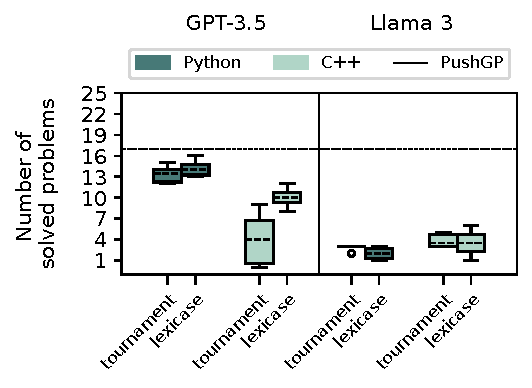
\includegraphics[width=\linewidth, trim={0mm 4mm 0mm 0mm}]{images/num_solved_problem_lexicase_psb2_6runs_boxplot_v5.pdf}
  \caption{PSB2.}
    % \vspace{14pt}
  \label{fig:num-solved-lexicase-selection-psb2}
\end{subfigure}
\begin{subfigure}{.45\linewidth}
\centering
\includegraphics[width=\linewidth, trim={0mm 4mm 0mm 0mm}]{images/num_solved_problem_lexicase_humaneval_6runs_boxplot_v5.pdf}
  \caption{HumanEval.}
  \label{fig:num-solved-lexicase-selection-he}
\end{subfigure}
\caption{Number of solved problems in lexicase and tournament selection experiments for SEIDR with GPT-3.5 and Llama 3 and fixed tree arity $N^*$.}
\label{fig:num-solved-lexicase-selection}
\end{figure}


\begin{figure}[bt]
\begin{subfigure}{.45\linewidth}
\centering
\includegraphics[width=\linewidth, trim={0mm 4mm 0mm 0mm}]{images/mean_tpr_lexicase_psb2_6runs_boxplot_v5.pdf}
  \caption{PSB2.}
  \label{fig:mean-tpr-lexicase-selection-psb2}
\end{subfigure}
\begin{subfigure}{.45\linewidth}
\centering
\includegraphics[width=\linewidth, trim={0mm 4mm 0mm 0mm}]{images/mean_tpr_lexicase_humaneval_6runs_boxplot_v5.pdf}
  \caption{HumanEval.}
  \label{fig:mean-tpr-lexicase-selection-he}
\end{subfigure}
\caption{Mean $TPR$ (measured in \%) in lexicase and tournament selection experiments for SEIDR with GPT-3.5 and Llama 3 and fixed tree arity $N^*.$}
\label{fig:mean-tpr-lexicase-selection}
\end{figure}

\begin{figure}[bt]
\centering
\includegraphics[width=\linewidth, trim={2mm 123mm 3mm 130mm}, clip]{images/best-avg-score-seidr-telo-humaneval-gpt-3.5-turbo-run3.pdf}
\caption{The best score on validation tests (y-axis) obtained up to an indicated logging step (x-axis) for problems solved from the second or later attempts with lexicase selection using SEIDR with GPT-3.5. Results are obtained for HumanEval. ``Step'' on the x-axis corresponds to logging settings and roughly indicates the speed of finding solutions to different problems. Each line stands for a unique solution.}
\label{fig:lexicase-tpr-jumps}
\end{figure}

\begin{highlight}
\textbf{Parent selection strategies for SEIDR with GPT-3.5 and Llama~3 in the generalizability experiments (\rqllama{}, \rqmultirun{}, \rqlexicase{}):} 
No leading ranking strategy is found for SEIDR experiments with GPT-3.5 and Llama~3 as measured by the average test pass rate and the average number of solved problems over six runs. 
In the vast majority of experiments where a solution is found and at least one debugging attempt is made the score jumps from 0 to 1 as opposed to climbing up incrementally and makes the ranking strategy less impactful than effective prompting. 
\end{highlight}


\begin{table}[t]
    \centering
    \caption{Average number of solved PSB2 problems using SEIDR with different LLMs and PushGP. The best results among SEIDR-only experiments at each $k$ are highlighted in bold. If pass@100 is not available, we cite the best available results in brackets. $N^*$ stands for the number of debug candidates and debug instructions to generate (tree arity).}\small
    \label{tab:generalizability-psb2}
\begin{tabular}{llllrrr}
\toprule
Language & Model in SEIDR & $N^*$ & Parent selection &  pass@1 &  pass@10 &  pass@100 \\
\midrule
% 
Python & GPT-3.5 & 1   &         tournament &    10.5 &     12.0 &      12.0 \\
    &        & 2   &         tournament &     9.3 &     11.5 &      12.0 \\
    &        & 4   &         tournament &     9.8 &     12.2 &      13.3 \\
    &        & 10  &         tournament &    10.7 &     \textbf{12.7} &      \textbf{14.5} \\
    &        & 16  &         tournament &    10.0 &     11.3 &      13.3 \\
    &        & 16  &           lexicase &    10.2 &     12.3 &      14.2 \\
    % &        & 100 &         tournament &    \textbf{10.8} &     12.2 &      13.7 \\
    &        & 100 &         tournament &    10.8 &     12.2 &      13.7 \\
\cline{3-7}\\[-8pt]
    &  \multicolumn{3}{l}{solved at least once by SEIDR with GPT-3.5} &  13 &       17 &       18 \\[1pt]
\cline{2-7}\\[-8pt]
        & Codex  & 10 & tournament &      5 &       10 &        14 (pass@1000=19) \\[1pt]
\cline{3-7}\\[-8pt]
       &  \multicolumn{3}{l}{solved at least once by SEIDR with Codex}   & 8 &       13 &        17 (pass@1000=20) \\[3pt]
\cline{2-7}\\[-8pt]
        &  PushGP (no SEIDR)   &    -            &       - &        - &       - &  (17)\\[1pt]
\cline{2-7}\\[-8pt]
% 
        & Llama~3 & 1   &         tournament &     1.2 &      1.3 &       2.3 \\
        &        & 2   &         tournament &     1.0 &      1.5 &       1.5 \\
        &        & 4   &         tournament &     1.0 &      1.5 &       2.3 \\
        &        & 10  &         tournament &     1.5 &      2.0 &       2.2 \\
        % &        & 16  &         tournament &     \textbf{1.7} &      \textbf{2.8} &       2.8 \\
        &        & 16  &         tournament &     1.7 &      \textbf{2.8} &       2.8 \\
        &        & 16  &           lexicase &     1.0 &      1.7 &       2.0 \\
        &        & 100 &         tournament &     1.0 &      1.0 &       \textbf{3.8} \\[1pt]
\cline{3-7}\\[-8pt]
    &  \multicolumn{3}{l}{solved at least once by SEIDR with Llama~3} &   4 &        5 &       11 \\
\midrule\\[-8pt]
 C++ & GPT-3.5 & 1   &         tournament &     0.0 &      5.6 &       5.5 \\
       &        & 2   &         tournament &     1.0 &      5.0 &       6.0 \\
       % &        & 2   &           lexicase &     \textbf{1.3} &     \textbf{ 9.0} &      \textbf{10.0} \\
       &        & 2   &           lexicase &     1.3 &     \textbf{ 9.0} &      \textbf{10.0} \\
       &        & 4   &         tournament &     1.0 &      4.6 &       6.8 \\
       &        & 10  &         tournament &     1.0 &      1.3 &       5.6 \\
       &        & 16  &         tournament &     1.0 &      1.2 &       8.3 \\
       &        & 100 &         tournament &     1.0 &      1.2 &       2.3 \\[1pt]
\cline{3-7}\\[-8pt]
       & \multicolumn{3}{l}{solved at least once by SEIDR with GPT-3.5}   & 2 &       13 &       13 \\[1pt]
% 
\cline{2-7}\\[-8pt]
   & Codex  & 10 & tournament &     3 &       12 &   14 (pass@1000=17)\\[1pt]
\cline{3-7}\\[-8pt]
       & \multicolumn{3}{l}{solved at least once by SEIDR with Codex}   & 10 &       12 &        15 (pass@1000=18) \\[1pt]
\cline{2-7}\\[-8pt]
   &  PushGP (no SEIDR) & -   &    -            &       - &        - &      (17)\\[1pt]
\cline{2-7}\\[-8pt]
        & Llama 3 & 1   &         tournament &     0.0 &      1.0 &       2.0 \\
       &        & 2   &         tournament &     0.0 &      \textbf{2.0} &       2.8 \\
       &        & 4   &         tournament &     1.0 &     \textbf{ 2.0} &       2.6 \\
       &        & 10  &         tournament &     1.0 &      1.4 &       \textbf{4.0} \\
       &        & 16  &         tournament &     0.0 &      1.8 &       3.8 \\
       &        & 16  &           lexicase &    1.0 &      1.4 &       3.5 \\
       &        & 100 &         tournament &     0.0 &      0.0 &       3.7 \\[1pt]
\cline{3-7}\\[-8pt]
       & \multicolumn{3}{l}{solved at least once by SEIDR with Llama~3}  & 4 &        5 &       11  \\
\bottomrule
\\ %% to make this a one
\\ %% page filling table
\end{tabular}
\end{table}


\begin{table}[t]
    \centering
    \caption{Percentage of solved tasks in HumanEval-X using SEIDR with different LLMs. The best results among SEIDR-only experiments at each $k$ are highlighted in bold. $N^*$ stands for the number of debug candidates and debug instructions to generate (tree arity).}\small
    \label{tab:generalizability-he}
\begin{tabular}{llllrrr}
\toprule
Language & Model in SEIDR & $N^*$ & Ranking &  pass@1 &  pass@10 &  pass@100 \\
\midrule
Python & GPT-3.5 & 1   &         tournament &    53.4 &     \textbf{60.4} &      63.3 \\
       &        & 2   &         tournament &    51.3 &     58.2 &      63.7 \\
       &        & 4   &         tournament &    52.1 &     58.4 &      64.8 \\
       &        & 4   &           lexicase &    52.5 &     59.6 &      \textbf{66.1} \\
       &        & 10  &         tournament &    51.1 &     58.3 &      61.7 \\
       &        & 16  &         tournament &    53.0 &     59.6 &      63.5 \\
       % &        & 100 &         tournament &    \textbf{54.0} &     56.7 &      62.5 \\[1pt]
       &        & 100 &         tournament &    54.0 &     56.7 &      62.5 \\[1pt]
\cline{3-7}\\[-8pt]
       & \multicolumn{3}{l}{solved at least once by SEIDR with GPT-3.5}   & 70.7 &     84.1 &      87.8 \\[1pt]
\cline{2-7}\\[-8pt]
    &   Llama 3 & 1   &         tournament &    22.0 &     44.0 &      47.1 \\
       &        & 2   &         tournament &    24.0 &     \textbf{48.5 }&      51.8 \\
       &        & 4   &         tournament &    22.5 &     43.1 &      51.8 \\
       &        & 10  &         tournament &    24.0 &     42.9 &      53.3 \\
       % &        & 10  &           lexicase &    \textbf{26.2} &     44.1 &      \textbf{54.1} \\
       &        & 10  &           lexicase &    26.2 &     44.1 &      \textbf{54.1} \\
       &        & 16  &         tournament &    23.5 &     41.6 &      51.5 \\
       &        & 100 &         tournament &    21.4 &     26.3 &      48.0  \\[1pt]
\cline{3-7}\\[-8pt]
       & \multicolumn{3}{l}{solved at least once by SEIDR with Llama~3} & 56.7 &     73.8 &      79.3 \\[1pt]
\cline{2-7}\\[-8pt]
& \multicolumn{6}{l}{\textbf{LLM results without SEIDR}} \\
 & GPT-3.5 (ChatGPT) & - &  - &  48.1  &  -   &    - \\
 & GPT-4 & - &  - & 67.0   &  -   &    - \\
 & Code Llama 34B & - &  - &  48.8  &  76.8   &    93.0 \\
 & Unnatural Code Llama 34B & - &  - &  62.2  &  85.2   &    95.4 \\
 & CodeGeeX & - &  - &  22.89  &  39.57   &    60.92 \\[-2pt]
\midrule\\[-10pt]
C++    & GPT-3.5 & 1   &         tournament &     3.4 &    \textbf{ 55.9} &      \textbf{78.5} \\
       % &        & 2   &         tournament &     \textbf{4.7} &     36.6 &      69.6 \\ 
       &        & 2   &         tournament &     4.7 &     36.6 &      69.6 \\
       &        & 2   &           lexicase &     4.3 &     35.9 &      73.6 \\
       &        & 4   &         tournament &     4.5 &     27.7 &      62.9 \\
       &        & 10  &         tournament &     3.6 &     13.7 &      49.7 \\
       &        & 16  &         tournament &     4.5 &     13.2 &      51.1 \\
       &        & 100 &         tournament &     3.6 &      7.1 &      31.3 \\[1pt]
\cline{3-7}\\[-8pt]
       & \multicolumn{3}{l}{solved at least once by SEIDR with GPT-3.5} & 20.1 &     89.0 &      99.4 \\[1pt]
\cline{2-7}\\[-8pt]
    &   Llama 3 & 1   &         tournament &    29.6 &     59.5 &      79.5 \\
    % &   Llama 3 & 1   &         tournament &    \textbf{29.6} &     59.5 &      79.5 \\
       &        & 2   &         tournament &    18.6 &     51.6 &      71.4 \\
       &        & 4   &         tournament &    20.0 &     50.6 &      73.9 \\
       &        & 10  &         tournament &    25.6 &     56.4 &      80.0 \\
       &        & 10  &           lexicase &    25.9 &     \textbf{60.9} &      \textbf{84.2} \\
       &        & 16  &         tournament &    20.9 &     53.0 &      75.5 \\
       &        & 100 &         tournament &    27.1 &     39.7 &      79.2 \\[1pt]
\cline{3-7}\\[-8pt]
       & \multicolumn{3}{l}{solved at least once by SEIDR with Llama~3} & 72.0 &     97.6 &      98.8  \\[1pt]
\cline{2-7}\\[-8pt]
& \multicolumn{6}{l}{\textbf{LLM results without SEIDR}} \\
& Code Llama 34B & - &  - &  47.8  &  -   &    - \\
& CodeGeeX & - &  - &  17.06  &  32.21   &    51.00 \\[-2pt]
\bottomrule
\end{tabular}
\end{table}

\subsubsection{Overall Generalizability of SEIDR with parent selection strategies and repair-replace trade-off.}
\label{sec:seidr-overall-generalizability}

We combine all results in Table~\ref{tab:generalizability-psb2} for PSB2 and Table~\ref{tab:generalizability-he} for HumanEval-X, where we show the number of solved problems at different cutoffs ($k$).  
An average is taken over all runs for the experiments with multiple restarts, and the results for one run are shown for SEIDR with Codex. 

Note that at cutoff $k=1$, iterations of SEIDR are not taken into account, because the first program candidate is the one LLMs generate from a template, and the trees at cutoff $k=1$ have only one program in each of them, regardless of the parent selection strategy or tree arity. 
Here, the difference between pass@1 results with different parent selection and tree arity is explained by the stochastic behavior of the underlying LLMs. 
We keep pass@1 results to inform the reader about the stochasticity of the models and for the ease of visual comparison of values in each row.

We compare the performance of PSB2 solutions synthesized with SEIDR to the PushGP genetic programming system with down-sampled lexicase selection~\cite{helmuth2022:problemsolving}. 
To compare the performance of SEIDR with other LLMs without SEIDR, we report the average percentage of solved problems for HumanEval-X. 
For HumanEval-X, we cite the performance of the state-of-the-art models as reported by their authors without SEIDR, such as CodeGeex~\cite{zheng2023:codegeex}, GPT-3.5 and GPT-4~\cite{openai2023:gpt4}, for reference, and compare SEIDR with GPT-3.5 and Code Llama~\cite{roziere2023:code} results at different cutoffs ($k$ for $pass@k$).
Furthermore, we report the number of solved problems in the union of all experiments for a given dataset, model, and language, because different problems are solved in different restarts of the method. 
We refer to these results as ``solved at least once'' hereafter.

In PSB2-Python experiments, SEIDR with Codex has a higher pass@1000 than the maximum pass@100 measured for SEIDR with GPT-3.5. SEIDR with Codex also solves 20 problems at least once, whereas SEIDR with GPT-3.5 solves 18.
SEIDR with Codex also outperforms other LLMs on PSB2 in C++.
No parent selection strategy or tree arity $N^*$ is leading across all PSB2 experiments. 

In the HumanEval-C++ experiments, SEIDR performs well at larger $k,$ i.e., when debugging steps are made. 
Remarkably, the union of SEIDR experiments with both GPT-3.5 and a much smaller Llama~3 solve 163 problems (or 99.4\% in Table~\ref{tab:generalizability-he}) and 162 problems (or 98.8\%) in HumanEval-C++, correspondingly.
SEIDR does not outperform other LLMs on HumanEval-Python, which, as mentioned earlier, could be the effect of HumanEval-Python being a popular benchmark for testing LLMs and indirectly optimizing the models.

Direct comparison of SEIDR results with other iterative program synthesis frameworks is challenging because, in addition to differences in benchmarks used, \cite{jiang2023:selfevolve} and \cite{chen2023:teaching} do not always report the number of generated programs, which is the primary metric that we use to compare iteration against a replace-only baseline.\footnote{\cite{chen2023:teaching} does have a sentence "Note that typically one debugging turn is sufficient"}


\begin{highlight}
\textbf{Summary of SEIDR results:} 
SEIDR with Codex benefits from the repair-replace trade-off when building a search tree of PSB2 solutions. The best results on PSB2 are achieved with Codex, tree arity of 10 and a maximum of 1000 programs generated. A trend of having the best tree arity set to 10 does not fully hold for other tested models, GPT-3.5 and Llama~3, where different tree arities performed better in different settings, e.g., depending on the parent selection algorithm, dataset, and programming language. 
Due to increasing costs of newer models time required for testing, we have run GPT-3.5 and Llama~3 six times with each set of hyperparameters and stopped building the search tree at 100 programs. 
In HumanEval-C++, the union of these runs has solved 163 problems with GPT-3.5, 162 problems with a much smaller Llama~3-8B model.
SEIDR runs have also solved 18 PSB2 problems in C++ and 20 in Python with Codex at least once in all the experiments. 
The numbers for SEIDR with GPT-3.5 are lower than for Codex, possibly due to the focus of GPT-3.5 on general reasoning and of Codex --- on coding.
A smaller Llama~3 model performs poorly on PSB2, which we appoint to the difficulty of the benchmark and the popularity of HumanEval and to the fact that the models can be indirectly optimized for higher performance on HumanEval than on other programming benchmarks.
\end{highlight}


\subsection{Threats to Validity}
\label{sec:seidr-threats}

External threats to validity concern SEIDR performance with benchmarks and language models different from those tested. 
Specifically, PSB2 and HumanEval-X contain programming tasks that require smaller functions to be generated than production-scale software.
Although some canonical solutions in HumanEval-Python have been criticised~\cite{liu2023:your}, we primarily use unit tests to evaluate the output of SEIDR and do not compute the exact match. Therefore, these weaknesses do not impact our results.
% We plan to extend our experiments in future work to explore the generalizability of results to more complex benchmarks.

Internal threats relate to the implementation.
We use PSB2, which has both corner cases and regular tests available. 
To ensure a fair comparison with other studies on PSB2, we evaluate and report results on the provided test set of PSB2, of which we randomly pick 2000 tests. 
A risk that a program does not pass tests other than the ones picked persists but is assumed to be low given the large enough number of 2000 tests. 

The large language models for code editing and text completion used in this study are non-deterministic, 
which can affect the results. 
Due to prohibitive model inference costs and discontinuation of support for earlier models, each experiment with Codex and GPT-3 is run only once. 
Experiments with Llama~3 and GPT-3.5 are restarted six times. 
We acknowledge that more restarts can provide a more complete picture of the approach performance,
although this is not the standard practice in the LLM domain~\cite{ouyang2023:llm} 
and can come at considerable financial and environmental costs.
Our temperature-based sampling procedure described in Section\ref{sec:seidr-synth} reduces this stochasticity significantly, especially for low-EPG results, because earlier solutions in the search tree are obtained with lower temperatures, and lower temperature limits the stochasticity.
Codex, GPT-3, and GPT-3.5 are black-box models and can generate malicious code~\cite{pearce2022:asleep}. 
Therefore, when coding in real life, the LLM output should be carefully reviewed before running it.
% \ag{The Codex model was pre-trained on an unbalanced dataset across programming languages~\cite{chen2021:evaluating}. Thus, 

The results can be skewed towards high performance in the programming languages prevailing in the pre-training dataset used by the authors of the tested LLMs -- an issue also known as \emph{data contamination}.
However, if the models were able to directly reproduce the solutions seen in the training data, 
these problems would have been solved from the first attempt.
Since we observe $EPG>1$ values, data contamination is likely to have only a partial effect on the results.
Moreover, the results can be affected by popular evaluation benchmarks: even though the benchmarks themselves are usually not parts of the pre-training dataset, the published LLMs are likely to be optimized for high performance on these benchmarks.   

\section{Conclusion}
\label{sec:seidr-conclusion}

In this study, we propose SEIDR, a multi-agent framework to solve the challenge of fully autonomous programming. 
In SEIDR, the program synthesis procedure is augmented from the direct generation of code with large language models instructions to iterative calls to a DEBUG agent followed by the RANK agent. 
The DEBUG agent performs a tree search across program candidates generated by a large language model for code.
The LLM used for code repair takes imperfect program candidates and instructions for their improvement as prompts. 
The instructions are obtained from both static templates with failing test case descriptions and templates with auto-generated bug summaries by a text completion language model. 

In addition to the initial exploration of hyperparameters that influence the population size at each generation and the number of children for each parent in SEIDR iterations, we extend the framework to test two different ranking strategies (tournament selection and lexicase selection), three models in the coding part of SEIDR (Codex, GPT-3.5 and Llama~3), two datasets (PSB2 and HumanEval-X), two programming languages (Python and C++), and various branching factors. 
With the update to newer models, the prompts and parameters of the tree search are updated accordingly. 

\paragraph{Contributions}
We run one set of initial exploration experiments and two sets of generalizability experiments. 
In the initial exploration, we test SEIDR with Codex-edit as the model for draft program synthesis and debugging in Python and C++ on the PSB2 benchmark. 
In our experiments, SEIDR outperforms the PushGP baseline and achieves the state-of-the-art result with 19 solved problems out of 25. 
It requires under 1000 program executions to solve them, in stark contrast to billions\footnote{~A problem is considered ``solved'' by PushGP if at least 1 of 100 runs, each with a limit of 60 million programs, was successful.} of executions in PushGP, making it feasible in the areas with costly testing, such as robotics.
Investigation of the repair-replace trade-off shows that SEIDR with tree arity of 10 outperforms both the replace-only strategy and the repair-only approach. 
% Our prompt engineering study shows that bug summaries generated with ``confidence indicators,'' such as ``obviously'' improve the performance of SEIDR during C++ code synthesis. 
% Overall, our framework shows low performance variability with different prompts, which indicates its robustness.%

To study the generalizability of SEIDR, we experiment with GPT-3.5 and Llama 3-8B as the models for draft program synthesis, explaining errors in synthesized programs and their debugging in Python and C++ on the PSB2 and HumanEval-X benchmarks. 
Our experiments with lexicase and tournament parent selection in the RANK agent do not show consistent improvement with either policy or any tree arity. 
One observation is that program candidates in generations prior to the final solution do not pass any test in the test suite in the vast majority of cases. 
The test pass rate for the final solution abruptly increases in one generation from 0 to all tests passed. 

In our generalizability experiments, SEIDR shows better performance than using LLMs without SEIDR with the same prompts and the same budget in terms of programs to generate.
The method achieves high results of 78.5\% average pass@100 on HumanEval-C++ with GPT-3.5 and 84.2\% with Llama~3.
Remarkably, in HumanEval-C++, the union of SEIDR restarts with different hyperparameters has solved 163 problems with GPT-3.5, 162 problems with a much smaller Llama~3-8B model.
The union of SEIDR runs has solved 18 PSB2 problems in C++ and 20 in Python with Codex. 
% Moreover, the method achieves the state-of-the-art result for pass@10 (74.44\%) with Code Llama 34B and for pass@100 (93.29\%) with GPT-3.5 on HumanEval-C++. 
% The approach requires under 100 program executions to obtain the reported results with GPT-3.5 and Code Llama.
% SEIDR with moderate number of generated programs for each bug explanation is favorable both for obtaining a solution and for the speed of solving a task. 

\paragraph{Future work}
Further investigation of SEIDR generalizability and ranking strategies are some of the areas for future work. 
Benchmarks with more tests than in HumanEval-X may shed more light on the most effective choice of the number of programs generated from each bug explanation, as well as the framework's comparison on large-context projects. 
As an agent-based framework, SEIDR shows how LLM-based agents and other non-LLM agents or components can collaboratively interact and solve software engineering tasks.

\section{Data Availability}
\todo{Replace with citeself}

To support open science and allow for replication and verification of our work, a replication package containing the code and results is publicly available in Zenodo.\footnote{~Zenodo DOI: \href{https://doi.org/10.5281/zenodo.13754705}{10.5281/zenodo.13754705}.
}
% \footnote{~While the manuscript is under review, the replication package is made available as a shared Google Drive to allow for improvements \url{https://drive.google.com/drive/folders/1SP0CVJQ6CdktFtksVs7tYu9jdLHIjHxa?usp=sharing}. We have reserved Zenodo DOI \href{https://doi.org/10.5281/zenodo.13754705}{10.5281/zenodo.13754705} to upload it after the review process has concluded.
% }


\newpage
\chapter{Multiagent Programming for Healthcare}\label{ch:seidrforhealth}

\newpage
\chapter{The Future} \label{ch:mimicseq}
\chapter{Imitation to optimization: MIMIC-SEQ} \label{ch:mimicseq}

\citeself{chapter}{liventsevIntensiveCareOne2024}

\section{Introduction}

\todo{Connect to other chapters}
\todo{Make sure there is an explicit research question}
\todo{Ensure standard nomenclature}

\paragraph{Intensive Care databases: a nano-review}
\label{sec:datasets}

% Why intensive care is a good source of data
Intensive Care is the medical speciality that supports patients whose lives are in immediate danger.
As such, it requires robust real time monitoring of the patient's vital signs due to quickly identify potential deterioration \cite{Bailey2013trial, Blount2010Real, Bockholt2022Real, Dimitrios1999Distributed, Fried2000Some, Mao2012integrated, Prgomet2016Vital, Vincent2018Improving}.
Monitoring hardware creates a datastream of variables like heart rate and blood oxygenation and, as a result, Intensive Care stands to benefit more than other fields of Healthcare from integration of data-driven models \cite{nunezreizBigDataAnalysis2019}.

% Datasets
MIMIC IV \cite{johnsonMIMICIVFreelyAccessible2023}, AmsterdamUMCdb \cite{amsterdamumcdb-a}, HiRID \cite{yecheHiRIDICUBenchmarkComprehensiveMachine} and the eICU Collaborative Research Database \cite{pollard2018a} are databases of health records obtained from Intensive Care Units.
Unlike many machine learning datasets, they avoid setting a standard for the parameters of the task such as which variables of a sample are to be used as features and which are to be predicted by the model, which samples are to be used for training and which are the holdout set - even what is a sample (a patient? an ICU admission? a drug? a diagnosis?). This makes them flexible and suitable for a wide array of tasks, but presents a challenge when seeking to compare different studies \cite{mcdermottReproducibilityMachineLearning2021}.

Derivative benchmarks, such as the MIMIC Benchmark \cite{harutyunyanMultitaskLearningBenchmarking2019} and HiRID-ICU-Benchmark \cite{yecheHiRIDICUBenchmarkComprehensiveMachine} seek to address the reproducibility issue: they put forth multiple datasets (one for each task) where all the information is derived from MIMIC and HiRID-ICU respectively, but is arranged specifically for the learning task at hand. They aim to become standard benchmarks for the tasks of mortality and length of stay prediction, patient fenotyping, prediction of circulatory, respiratory or kidney failure.

\paragraph{Towards foundation models for Healthcare}

Generalist models have demonstrated a superior performance to task specific models in many areas of machine learning \cite{reedGeneralistAgent2022} due to their ability to exploit implicit shared subtasks. 
This finding has precipitated the birth of a new paradigm known as foundation models \cite{zhouComprehensiveSurveyPretrained2023} - models trained on an all-encompassing dataset (such as the dataset that attempts to approximate all written text \cite{chelbaOneBillionWord2013}) and designed to be adapted to a broad array of specific downstream tasks.

The learning tasks typically studied in Healthcare are often interrelated. 
To use an example from section \ref{sec:datasets}, sepsis presents a high risk of death \cite{schlichtingRecognizingManagingSevere2007} and predicting sepsis is evidently useful for predicting mortality.
In light of existing research on generalist models, it is likely that considering them separately is counterproductive.
This, together with the vital societal importance of access to healthcare amidst understaffing \cite{ashleyy.metcalfHospitalUnitUnderstaffing2016, hudsonUnderstaffing2015, mercerMessageEditorinChief2008, munnUnderstaffingWardsCompromising2017, r.stanleyUnderstaffedOverwhelmed2010, SurveyShowsHidden1993, thelancetHealthcareSystemStaffing2018, UnderstaffingSignificantIssue2012} and population ageing \cite{2012health, Aslam2021Ageing, L1991aging, Lloyd2012Population, Mahishale2015Ageing, Mann2004aging, Sammy2019global, Suzman2015Health}, makes a foundation model for Healthcare a particularly important research goal.

\paragraph{Healthcare as Sequence Modeling}
\label{sec:sequencemodel}

With a few notable exceptions foundation models tend to be sequence models: estimating the probability a sequence of fixed-size elements

\begin{equation}
    \hat{p}(t_1, \dots, t_n)
\end{equation}

typically modeled as conditional probability of one (usually last) element given others

\begin{equation}
    \hat{p}(t_n | t_1, \dots, t_n)
\end{equation}

since most tasks in machine learning can be represented as sequence modeling. 
There is evidence that this generality is a fundamental property of sequence models: see proofs that Recurrent Neural Networks \cite{siegelmannComputationTuringLimit1995} and Attention \cite{perezAttentionTuringComplete} are Turing-complete.

One of the tasks that has recently been reimagined as a Sequence Modeling task is Reinforcement Learning and Healthcare has a Reinforcement Learning interpretation: it's an interaction between the doctor (the agent) and the patient's body (the environment) that has all the trappings of a POMDP: the treatment interventions are actions $a_n$ and the observable vital signs are observations $o_n$.
Consider a \emph{trajectory} in a Partially Observable Markov Decision Process, i.e. a history of actions $a$, observations $o$ and rewards $r$:

\begin{equation}
    \tau = (o_1, a_1, r_1, o_2, a_2, r_2, o_3, a_3, r_3, \dots)
\end{equation}

A model $\hat{p}$ that can predict the next element in a trajectory can be used as a \emph{dynamics model} to predict the next observation from the patient:

\begin{equation}
    o_{n+1} \sim \hat{p}(o_{n+1} | \dots, o_n, a_n, r_n)
\end{equation}

as an \emph{imitative policy} to predict which intervention the doctor will choose next

\begin{equation}
    a_{n+1} \sim \hat{p}(a_{n+1} | \dots a_n, r_n, o_{n+1})
\end{equation}

or, after an additional optimization step, as an \emph{optimal policy} to predict which intervention the doctor \emph{should} choose next.
For a planning horizon of 1 (greedy policy) it is defined as:

\begin{equation}
    a_{n+1} = \arg \max_a \mathbb{E} [r_{n+1} \sim \hat{p}(r_{n+1} | \dots a_n, r_n, o_{n+1}, a)]
\end{equation}

Thus while the paradigm of Healthcare as a Sequence Modeling task is novel, there is a robust body of research reducing Healthcare to Reinforcement Learning \cite{yuReinforcementLearningHealthcare2021} and Reinforcement Learning to Sequence Modeling \cite{chenDecisionTransformerReinforcement2021, jannerOfflineReinforcementLearning2021, schmidhuberReinforcementLearningUpside2020}. 

\paragraph{Contributions}

In this paper we introduce
\begin{itemize}
    \item the paradigm of Healthcare as Sequence Modeling
    \item MIMIC-SEQ: a benchmark dataset for Sequence Models of Intensive Care derived from MIMIC-IV
    \item Evaluation guidelines for a holistic comparison of intensive care forecasting models
    \item An MLP-based baseline model
\end{itemize}

\newpage
\section{Related Work}

\cite{weiMIMICELMIMICIVEvent2022} develop MIMICEL, a linearized event sequence representation of MIMIC-IV-ED \cite{johnsonMIMICIVED2021} emergency department dataset for downstream application in machine learning and process mining. 
However, MIMIC-IV-ED is a smaller dataset than MIMIC-IV, and \cite{weiMIMICELMIMICIVEvent2022} stop short of releasing a full benchmark suite with an evaluation procedure and baselines.
Incorporating MIMICEL into MIMIC-SEQ would be a fruitful direction of future research.
Similarly to our approach,
\cite{kuznetsovaImportanceStepwiseEmbeddings2023} and \cite{tipirneniSelfSupervisedTransformerSparse2022} represent intensive care data as an irregular event stream timeseries, however they still rely on manual selection of important variables and prediction targets.

\section{MIMIC-SEQ}
\label{sec:dataset}

MIMIC-SEQ is a dataset for training foundational models for Intensive Care in the Sequence Modeling paradigm derived from MIMIC-IV.
It sets out a single machine learning task, with fully standardized train and test sets for reproducible comparisons between methods, while, at the same time, the task is so general that if a model accomplishes it successfully, this model can be used without fine-tuning for many narrow tasks, including mortality and length of stay prediction.
We also provide a suite of evaluation metrics and 2 baseline models.

%\begin{figure}
%    \centering
%     \begin{subfigure}[b]{0.5\textwidth}
%         \includegraphics[width=\textwidth]{relationships.real.compact.png}
%         \caption{SQL schema of MIMIC}
%         \label{fig:mimic-schema}
%    \end{subfigure}
%     \hfill
%     \begin{minipage}[b]{0.45\textwidth}
%         \begin{subfigure}[b]{0.7\linewidth}
%             \includegraphics[width=\textwidth]{schema.drawio.png}
%             \caption{SQL schema of MIMIC-SEQ}
%             \label{fig:mimic-schema}
%         \end{subfigure}
%    \end{minipage}
%end{figure}

\newpage
\section{Building the timeseries dataset}

\begin{figure}
    \centering
    \includegraphics[width=0.8\linewidth]{mimiciv.png}
    \caption{Entity-Relationship diagram of MIMIC-IV}
    \label{fig:mimic}
\end{figure}

For every patient admission recorded in MIMIC-IV we collect all related information from various heterogeneous subdatasets, namely,

\begin{itemize}
    \item ICU input events (\texttt{inputevents})
    \item ICU procedures (\texttt{procedureevents})
    \item Hospital prescriptions (\texttt{prescriptions})
    \item Patient admissions and demographics (\texttt{admissions} and \texttt{patients})
    \item ICU charted events (\texttt{chartevents})
    \item Hospital lab events (\texttt{labevents})
    \item Microbiology tests (\texttt{microbiologyevents})
    \item Procedures coded in ICD format (\texttt{procedures\_icd})
    \item Healthcare Common Procedure Coding System (HCPCS) events (\texttt{hcpcsevents})
    \item Electronic medication administration records (eMAR) (\texttt{emar})
\end{itemize}

Every patient history is then represented as a sequence of events where each event has:
\begin{enumerate}
    \item a type (each type has an associated text label, i.e, "Penatal given")
    \item time when it happened
    \item (optionally) intensity
\end{enumerate}

Intensities may represent dosages of drugs or other quantitative measures (charted heart rate, blood pressure, patient age).

Events that have a duration, such as medication administrations, are recorded as 2 events: "start X" and "end X". 
Demographic information, including ethnicity, gender, and age, is recorded as a dummy event ocurring the time of admission.

\paragraph{Resulting dataset}

\begin{figure}
    \centering
    \includegraphics[width=0.7\linewidth]{mimicseq.png}
    \caption{Entity-Relationship diagram of MIMIC-SEQ}
    \label{fig:enter-label}
\end{figure}

\begin{table}[H]
    \centering
    \scriptsize
    \begin{tabular}{c|r|l}
    eventtime &	label &	intensity \\
    2185-08-13T16:57:00 &	WHITE	 & \\
    2185-08-13T16:57:00 &	AGE &	18.0 \\
    2185-08-13T16:57:00 &	URGENT ADMISSION &	 \\
    2185-08-13T16:57:00 &	FEMALE &	 \\
    2185-08-13T21:00:00 &	Start Prenatal Vitamins Tablet prescription, PO &	1.0 \\
    2185-08-13T22:00:00 &	Start LORazepam 1mg Tablet prescription, PO/NG &	 \\
    2185-08-13T22:00:00 &	Start HydrOXYzine 25 mg Tab prescription, PO/NG &	 \\
    2185-08-14T08:00:00 &	Start Complera 200 mg-25 mg-300 mg tablet prescription, ORAL &	1.0 \\
    2185-08-14T17:00:00 &	Start Acetaminophen 325mg Tablet prescription, PO/NG &	 \\
    2185-08-19T11:30:00 &	DISCHARGE TO HOME &	 \\
    2185-08-19T18:00:00 &	Stop LORazepam 1mg Tablet prescription, PO/NG &	 \\
    2185-08-19T18:00:00 &	Stop Prenatal Vitamins Tablet prescription, PO &	1.0 \\
    2185-08-19T18:00:00 &	Stop HydrOXYzine 25 mg Tab prescription, PO/NG &	 \\
    2185-08-19T18:00:00 &	Stop Complera 200 mg-25 mg-300 mg tablet prescription, ORAL &	1.0 \\
    2185-08-19T18:00:00 &	Stop Acetaminophen 325mg Tablet prescription, PO/NG &	 \\
    \end{tabular}
    \caption{An (unusually short) hospital admission from MIMIC-SEQ}
\end{table}

MIMIC-SEQ contains 481374190 clinical events in 522740 train and 10000 test episodes (hospital admissions).

\begin{table}[H]
    \centering
    \begin{tabular}{c|c|c|c}
         & min & avg & max \\
         Events per episode & 4 & 919 & 564721 \\
         Episode duration & 0 & 6 days & 68 years \\
    \end{tabular}
    \caption{Dataset statistics}
    \label{tab:stats}
\end{table}

It is publicly available, subject to (no cost, open to everyone) MIMIC-IV data use agreement.
See the dataset repository.

\paragraph{Clustering}

87899 event types is a very fine-grained view of the intensive care scenario that differentiates, for example, between different versions of the same drug (say, pills and tablets).
This is done intentionally to pave the way for sophisticated models, however, we recognize that a simplified version of the task can be helpful.
To that end, we enrich the dataset with 4 \emph{clusterings}: c10, c100, c1000 and c10000.
They are achieved by embedding each event type label with OpenAI's \emph{ada2} embedding model and running a k-means clustering algorithm in the induced latent space.
As a result, one can train a model for simplified \emph{clustered} versions the task making predictions in terms of broad event categories, not individual event types.

\paragraph{Evaluation guidelines}

We suggest evaluating forecasting models on 2 test tasks using the holdout patient histories:
\begin{description}
    \item[second day prediction] for every episode in the holdout set, use all events within 24 hours of the very first event as model input. Use the next 24 hours as expected output.
    \item[last day prediction] for every episode in the holdout set, use all events within 24 hours of the very last event as expected output. Use the rest of the events as model input. 
\end{description}

Each of the two can in turn be decomposed into:
\begin{description}
    \item[event prediction task] which events will happen and which will not?
    \item[intensity prediction task] if the event happens, what will be its intensity?
\end{description}

The former is a \emph{binary classification task} with metrics like \emph{accuracy}, \emph{precision} and \emph{recall}.
Note that it's a highly imbalanced binary classification task and, as such, relying on accuracy is not recommended - \emph{f1 score}, \emph{kappa} or \emph{dice score} shall be used instead.
The latter is a \emph{regression task} and the recommended metric is $R^2$ coefficient.

\emph{Event prediction} can be done in the space of concrete events or in the space of clusters c10, c100, c1000, c10000.
So, in total, a model evaluation includes 10 binary classification tasks (second day prediction and last day prediction for each event granularity) and 2 regression tasks.

\paragraph{Relationship to existing benchmarks}

A predictive model trained on \emph{MIMIC-SEQ} can perform the standard tasks used in current benchmarks \cite{harutyunyanMultitaskLearningBenchmarking2019}, such as
\begin{itemize}
    \item \emph{length of stay prediction} by estimating the probability of \texttt{DISCHARGE TO HOME} \\ \texttt{DISCHARGE TO REHAB} \\ \texttt{DISCHARGE TO HEALTHCARE FACILITY} \\ \texttt{DISCHARGE TO PSYCH FACILITY}\\\texttt{DISCHARGE TO OTHER FACILITY}\\\texttt{DISCHARGE TO REHAB}\\\texttt{DISCHARGE TO ASSISTED LIVING}\\\texttt{DISCHARGE TO HOSPICE}\\\texttt{DISCHARGE TO ACUTE HOSPITAL}\\\texttt{DISCHARGE AGAINST ADVICE} \\ \texttt{DISCHARGE TO HOME HEALTH CARE} \\ \texttt{DISCHARGE TO CHRONIC/LONG TERM ACUTE CARE} \\ \texttt{DISCHARGE TO SKILLED NURSING FACILITY} \\ \texttt{DISCHARGE TO DIED} \\ events over different timescales
    \item \emph{mortality prediction} by estimating the probability of \texttt{DISCHARGE TO DIED} relative to other types of discharge
    \item \emph{decompensation prediction} by estimate the probability of \texttt{DISCHARGE TO DIED} within 24 hours and/or events known to signify an acute increase in letality
    \item \emph{phenotyping} by estimating the probability of various \texttt{DISEASE X DIAGNOSED} events
\end{itemize}

as well as many others.

\newpage
\section{Baseline}
\label{sec:baseline}

Our baseline model consists of a two-layer multilayer perceptron (MLP) with 1000 hidden layer size RELU \cite{agarapDeepLearningUsing2018} activation function and batch normalization after each layer. As input, all events from the first day are used and one-hot encoded in a 87899-dimensional vector. As prediction target, all events from the second day are used and encoded via their clustering mapping, e.g. c10, c100, c1000, c10000, into a vector of the corresponding dimension. As objective function we used binary cross entropy. The last layer contains a sigmoid function which transforms the output to probabilities for each vector element. A threshold is set at 0.5 to decide if an event occurs or not. All models were trained with batch size 512 for 3 epochs.

We test our baseline on the \emph{second day event prediction task} and summarize the results for different clusterings in table \ref{tab:mytable2}. It can be seen that the more classes are in the clustering, the harder the prediction task becomes. As noted above, accuracy is a deceptive metric in this scenario.

\begin{table}[H]
  \centering
    \begin{tabular}{lcccc} \toprule
        {clustering} & {recall} & {accuracy} & {precision} & {F1}  \\ \midrule
        {c10}  & 0.903 & 0.840 & 0.790 & 0.827 \\
        {c100}  & 0.568 & 0.885 & 0.713 & 0.632 \\
        {c1000}  & 0.500  & 0.976 & 0.710  & 0.586 \\
        {c10000}  & 0.509  & 0.996 &  0.703  & 0.589 \\ \midrule
%        {average performance}  & \textbf{0.598}  & -0.597 & 0.598  & 0.052 \\ \bottomrule
    \end{tabular}
  \caption{Evaluation results of 2 x 1000 MLP for first day - second day  prediction, entire dataset}
  \label{tab:mytable2}
\end{table}



For many patients it is the case that they are in the hospital for only one day. For these patients, the model should predict no event on the second day. However, evaluation of the models showed that this is almost never the case. However, one can argue that it is more important to get problematic patients correct than the ones who leave the hospital after one day. Therefore, we evaluated the model also only on patients which are in the hospital for at least 2 days. Since the data is roughly ordered according to length of stay, we achieved this by skipping the first 100k samples in the training and the first 1k samples in the test data. The models shows improved performance here, as can be seen in Table \ref{tab:mytable1}.


\begin{table}[H]
  \centering
    \begin{tabular}{lcccc} \toprule
        {clustering} & {recall} & {accuracy} & {precision} & {F1}  \\ \midrule
        {c10}  & 0.942  & 0.854 & 0.850  &  0.890 \\ 
        {c100}  & 0.633  & 0.878 & 0.765  &  0.692 \\ 
        {c1000}  & 0.548  & 0.974 & 0.770  &  0.640 \\ 
        {c10000}  &  0.539  & 0.995 & 0.771  &  0.634 \\ \midrule
        
%        {average performance}  & \textbf{0.598}  & -0.597 & 0.598  & 0.052 \\ \bottomrule
    \end{tabular}
  \caption{Evaluation results of 2 x 1000 MLP for first day - second day  prediction, skipping first 100k train / 1k test samples}  \label{tab:mytable1}
\end{table}


%\begin{table}[h]
%  \centering
%    \begin{tabular}{lcccc} \toprule
%        {c10000} & {recall} & {accuracy} & {precision} & {F1}  \\ \midrule
%        {entire dataset}  & 0.495  & 0.996 & 0.711  &  0.583 \\ \midrule
%        {average performance}  & \textbf{0.598}  & -0.597 & 0.598  & 0.052 \\ \bottomrule
%    \end{tabular}
%  \caption{Evaluation results of 2 x 1000 MLP for first day - second day  prediction with c10000 for different subsets, run again!}  \label{tab:mytable}
%\end{table}

The same setup but with 3 hidden layers and 5000 units each shows improved performance as can be seen in table \ref{tab:mytable3}. Bigger models were tested as well, but showed no further improvement.


\begin{table}[H]
  \centering
    \begin{tabular}{lcccc} \toprule
        {configuration} & {recall} & {accuracy} & {precision} & {F1}  \\ \midrule
        {1}  & 0.505  & 0.996 &  0.727  & 0.595 \\
        {2} & 0.544  & 0.9959 &  0.784  & 0.642 \\  \midrule
%        {average performance}  & \textbf{0.598}  & -0.597 & 0.598  & 0.052 \\ \bottomrule
    \end{tabular}
  \caption{All evaluations with c10000; 1: Evaluation results of 3 x 5000 MLP for first day - second day  prediction, entire dataset; 2: Evaluation results of 3 x 5000 MLP for first day - second day prediction, skip first 100k train / 1k test samples}
  \label{tab:mytable3}
\end{table}




Replacing ones in the one-hot encoding with the corresponding events' intensities impaired the models' performance, likely because it introduces a false equivalency between a zero-intensity event and lack of an event, i.e. "average blood pressure" is different from "no blood pressure measurement".

% \begin{table}[h]
%   \centering
%     \begin{tabular}{SSSSSSSS} \toprule
%         {clustering} & {recall} & {accuracy} & {precision} & {F1}  \\ \midrule
%         {c10000}  & 0.339  & 0.995 &  0.687  & 0.452 \\ \midrule
% %        {average performance}  & \textbf{0.598}  & -0.597 & 0.598  & 0.052 \\ \bottomrule
%     \end{tabular}
%   \caption{Evaluation results of 2 x 1000 MLP for first day - second day  prediction, 500k dataset with intensity values}
%   \label{tab:mytable}
% \end{table}


\newpage
\section{Conclusion}

Narrow tasks in machine learning for intensive care have been a result of technical limitations that have become less relevant with recent advances in the field. 
We propose a more general approach, publish a dataset to support it and demonstrate its viability with a simple baseline model.
The long term ambition of this work is to become the basis for training foundation models of intensive care using modern neural network architectures.
Of particular interest are Transformers \cite{vaswaniAttentionAllYou2023}, Neural Controlled Differential Equations \cite{kidgerNeuralControlledDifferential2020} and Structured State Space Models \cite{guEfficientlyModelingLong2022}.

\newpage
\chapter{Reproducibility and software artefacts}

\chapter{Reproducibility and software artefacts}

\section{FizzBuzzLM}

\section{Cibi}

\section{tree2tree}

\section{programlib}

\section{SEIDR}

\section{imagym}

\section{Auto-ALS}



\newpage
\chapter{Acknowledgments}

\epigraph{Стёр строк больше, чем выдал Джон Гришам \\ Нос тёр жёстче разве что Жижек}{Oxxxymiron}

This project has received funding from European Union’s Horizon 2020 research and innovation programme under grant agreement n° 812882. 

Parts of this text were converted from spoken audio with the use of English-only medium size OpenAI Whisper model \cite{radfordRobustSpeechRecognition2022}

\printbibliography

\end{document}
